% Options for packages loaded elsewhere
\PassOptionsToPackage{unicode}{hyperref}
\PassOptionsToPackage{hyphens}{url}
%
\documentclass[
]{book}
\usepackage{amsmath,amssymb}
\usepackage{lmodern}
\usepackage{iftex}
\ifPDFTeX
  \usepackage[T1]{fontenc}
  \usepackage[utf8]{inputenc}
  \usepackage{textcomp} % provide euro and other symbols
\else % if luatex or xetex
  \usepackage{unicode-math}
  \defaultfontfeatures{Scale=MatchLowercase}
  \defaultfontfeatures[\rmfamily]{Ligatures=TeX,Scale=1}
\fi
% Use upquote if available, for straight quotes in verbatim environments
\IfFileExists{upquote.sty}{\usepackage{upquote}}{}
\IfFileExists{microtype.sty}{% use microtype if available
  \usepackage[]{microtype}
  \UseMicrotypeSet[protrusion]{basicmath} % disable protrusion for tt fonts
}{}
\makeatletter
\@ifundefined{KOMAClassName}{% if non-KOMA class
  \IfFileExists{parskip.sty}{%
    \usepackage{parskip}
  }{% else
    \setlength{\parindent}{0pt}
    \setlength{\parskip}{6pt plus 2pt minus 1pt}}
}{% if KOMA class
  \KOMAoptions{parskip=half}}
\makeatother
\usepackage{xcolor}
\usepackage{longtable,booktabs,array}
\usepackage{calc} % for calculating minipage widths
% Correct order of tables after \paragraph or \subparagraph
\usepackage{etoolbox}
\makeatletter
\patchcmd\longtable{\par}{\if@noskipsec\mbox{}\fi\par}{}{}
\makeatother
% Allow footnotes in longtable head/foot
\IfFileExists{footnotehyper.sty}{\usepackage{footnotehyper}}{\usepackage{footnote}}
\makesavenoteenv{longtable}
\usepackage{graphicx}
\makeatletter
\def\maxwidth{\ifdim\Gin@nat@width>\linewidth\linewidth\else\Gin@nat@width\fi}
\def\maxheight{\ifdim\Gin@nat@height>\textheight\textheight\else\Gin@nat@height\fi}
\makeatother
% Scale images if necessary, so that they will not overflow the page
% margins by default, and it is still possible to overwrite the defaults
% using explicit options in \includegraphics[width, height, ...]{}
\setkeys{Gin}{width=\maxwidth,height=\maxheight,keepaspectratio}
% Set default figure placement to htbp
\makeatletter
\def\fps@figure{htbp}
\makeatother
\setlength{\emergencystretch}{3em} % prevent overfull lines
\providecommand{\tightlist}{%
  \setlength{\itemsep}{0pt}\setlength{\parskip}{0pt}}
\setcounter{secnumdepth}{5}
\usepackage{booktabs}
\ifLuaTeX
  \usepackage{selnolig}  % disable illegal ligatures
\fi
\usepackage[]{natbib}
\bibliographystyle{plainnat}
\IfFileExists{bookmark.sty}{\usepackage{bookmark}}{\usepackage{hyperref}}
\IfFileExists{xurl.sty}{\usepackage{xurl}}{} % add URL line breaks if available
\urlstyle{same} % disable monospaced font for URLs
\hypersetup{
  pdftitle={표준운영절차서},
  pdfauthor={관할해역공동활용체계구축(2단계) (JOISS)},
  hidelinks,
  pdfcreator={LaTeX via pandoc}}

\title{표준운영절차서}
\author{관할해역공동활용체계구축(2단계) (JOISS)}
\date{2023-04-18}

\begin{document}
\maketitle

{
\setcounter{tocdepth}{1}
\tableofcontents
}
\hypertarget{intro}{%
\chapter{intro}\label{intro}}

안녕하세요

\hypertarget{ctdsbe-911plusuxb97c-uxc774uxc6a9uxd55c-uxd574uxc218-uxc555uxb825uxce21uxc815-uxd45cuxc900uxc6b4uxc601uxc808uxcc28uxc11c}{%
\chapter{CTD(SBE 911plus)를 이용한 해수 압력측정 표준운영절차서}\label{ctdsbe-911plusuxb97c-uxc774uxc6a9uxd55c-uxd574uxc218-uxc555uxb825uxce21uxc815-uxd45cuxc900uxc6b4uxc601uxc808uxcc28uxc11c}}

\hypertarget{uxae30uxbcf8-uxb3d9uxc791uxc6d0uxb9ac}{%
\section{기본 동작원리}\label{uxae30uxbcf8-uxb3d9uxc791uxc6d0uxb9ac}}

SBE 911plus CTD는 미국 Sea-Bird Electronics 사에서 제작한 장비로 세계에서 가장 널리 사용되고 있으며, 특히 WOCE(World Ocean Circulation Experiments)의 표준장비로 사용되고 있다(Kim et al,2000). 이 장비는 바다 속에서 관측하는 부분인 SBE 9plus underwater unit (main housing, pump and sensors)와 CTD 제어, 자료수신, 전원공급을 하는 SBE 11 deck unit로 구성되어 있다. 특히, deck unit 부분에는 water sampler를 제어하는 button이 있어, 관측시에 원하는 수심에서 해수를 채수할 수 있다. 이 장비는 자료를 초당 24회의 속도로 획득한다. SBE 9plus의 구성은 그림 1과 같고 제원은 다음 표1과 같다.

이 장비는 수온과 전도도를 측정하기 위해서 SBE 5T 또는 SBE 5P 펌프를 이용하여 해수를 일정한 유속(30 ㎤/s)으로 직경 0.4 ㎝의 T-C duct 입구를 통해 온도센서와 전도도셀을 순차적으로 통과시킨다. 펌프를 사용하는 장점은 수중에서 CTD의 움직임과 상관없이 해수가 일정한 속도로 센서와 접촉할 수 있게 한다. 일단 해수가 T-C duct로 유입되면 수온이 즉시 감지되고 duct를 통해 해수가 흘러 0.073초후에 conductivity cell로 들어간다. 펌프의 속도가 고정되어 있기 때문에 온도센서와 전도도센서 사이의 지연시간(0.073초)은 항상 일정하고, SBE 11plus Deck Unit에서 실시간으로 자동 보정된다.

\hypertarget{uxc7a5uxbe44uxad6cuxc131}{%
\section{장비구성}\label{uxc7a5uxbe44uxad6cuxc131}}

\hypertarget{uxc8fcuxc694uxc13cuxc11c}{%
\subsection{주요센서}\label{uxc8fcuxc694uxc13cuxc11c}}

\hypertarget{uxc218uxc628uxc13cuxc11c}{%
\subsubsection{수온센서}\label{uxc218uxc628uxc13cuxc11c}}

수온센서의 측정원리는 수온이 변화할 때 저항(resistance)이 변하며, thermistor의 저항에 따라 주파수(즉, signal)이 달라지는 원리로 측정된다. 그러나, 따뜻한/고인 찬물에서 찬/따뜻한 물로 주변 환경이 바뀔 때, 따뜻한/찬 환경에 있을 때 존재한 thermistor 내부의 열이 찬/따뜻한 주변 환경으로 확산되는 데 시간이 필요하게 된다. 흔히 이러한 time constant(step change가 주어질 때, 센서가 최종값의 약 63\%에 도달하는데 걸리는 시간)은 약 70ms(0.070초)로 알려져 있다. SBE9plus underwater unit의 경우에 24Hz, 즉 0.0417초마다 측정하므로 이에 대한 보정은 흔히 생략된다. 아래 표는 Sea bird 제조사에서 권장하는 장비별 전형적인 수온센서 배열시간이다. Data processing 프로그램의 Alignctd 과정에서 보정을 하게 된다.

\hypertarget{uxc804uxae30uxc804uxb3c4uxb3c4-uxc13cuxc11c}{%
\subsubsection{전기전도도 센서}\label{uxc804uxae30uxc804uxb3c4uxb3c4-uxc13cuxc11c}}

전기전도도 센서의 셀은 약 2 cm3의 부피를 갖으며, 30 ㎖/s의 양으로 펌프의 작동에 의해 플러싱될 때 이러한 부피는 약 67ms의 시간이 소요된다. 전기전도도의 변화에 따른 셀의 time constant는 약 24ms(0.024s)로 알려져 있다. 그러나 이러한 전기전도도 셀의 특징에 의한 반응시간 보다는 아래의 그림처럼 전기전도도와 수온이 동시에 관측되지 않는 이유로 인한 두 센서간의 반응시간 차이가 중요하다. 전기전도도로부터 계산되는 염분은 수온, 전기전도도, 압력의 함수이기 때문에 정확한 염분계산을 위해서는 수온과 전기전도도의 동시 측정이 필요하다. 그러나 해수는 수온센서를 통과한 후에 전기전도도 센서를 통과하므로 이러한 차이를 보정하기 위한 과정이 필요하다. SBE11plus deck unit는 전기전도도와 수온센서간의 전형적인 시간차가 0.073 초이므로, primary 전기전도도 센서에 대하여 +1.75scans(24Hz에서 1.75/24=0.073 seconds) 만큼 factory-set를 하고 있지만, 주로 수온변화가 급격한 thermocline에서 매 관측시마다 차이(-0.08초\textasciitilde0.08초)를 보이므로 시간차에 대한 정확한 계산이 필요하다. 시간차에 대한 정확한 보정은 염분 값에 나타나는 튐 현상을 대부분 보정할 수 있다. 이 매뉴얼의 alignctd 과정에서 자세히 설명하기로 한다.

\hypertarget{uxc555uxb825uxc13cuxc11c}{%
\subsubsection{압력센서}\label{uxc555uxb825uxc13cuxc11c}}

반도체 물질에서 압전저항 효과는 (piezoresistive effect) 결정구조의 변화에 의한 전기저항 변화를 브리지 회로를 통해 평가한다. 온도변형에 따라 저항변화가 일어나기 때문에 측정기가 동일한 저항을 가지게 하기 위해 동일한 기하 모양으로 배열하고 온도를 정밀하게 측정하여 보정해 주어야 한다. 반도체 물질에서 압전저항 효과는 금속변형율 측정기보다 약 50배 정도 더 민감하다. 압전저항 압력변환기는 일반적인 반도체 제조 방밥으로 수행하고 있고, 압력하에서 변형되는 탄성 멤브레인과 저항기를 하나의 칩에 통합할 수 있어 전체 압력 측정 셀이 한 개의 칩으로 구성되어 있어 아주 작은 크기로 만들 수 있다. SBE 9plus에 사용된 압력센서는 Paroscientific사의 Digiquartz 압력센서이다. 이 센서는 압력에의한 변형이 정밀한 수정결정 공명의 진동주기를 변화시키고, 진동주기 변화가 정밀시계 와 계수기에 사용되는 진동전자에 의해 측정된다.

\hypertarget{uxc6a9uxc874uxc0b0uxc18c-uxc13cuxc11c}{%
\subsubsection{용존산소 센서}\label{uxc6a9uxc874uxc0b0uxc18c-uxc13cuxc11c}}

해수 중 용존산소는 측정하는 SBE 43 센서는 아래 그림과 같이 해수가 센서의 membrane 표면으로 먼저 확산된 후, electrode를 덮고 있는 Teflon membrane을 통하여 확산되어진 후 electrode 위의 electrolyte로 확산되어 진다. 이때 electrode 표면에서 화학적인 반응이 발생하며, 이러한 확산율은 수온에 의존하게 되므로 센서의 반응시간은 수온의 함수이다. 일반적으로 20℃ 수온에서 time constant(τ)는 약 2초로 알려져 있으나, sensor와 membrane의 조건과 age에 따라 달라진다.

\hypertarget{uxbc30uxc5f4-uxbc29uxc2dd}{%
\subsection{배열 방식}\label{uxbc30uxc5f4-uxbc29uxc2dd}}

SBE 9plus는 기본적으로 수직 상태로 사용되지만 SBE 32 Carousel Water Sampler와 같이 사용할 때는 수평 상태로 사용된다. 수직배치(horizontal mount)와 수평배치(vertical mount)의 펌프 위치나 배관은 다르며, 펌프와 배관이 적절하게 배열되지 않으면 공기가 갇히거나 펌프가 잘 작동되지 않는 문제가 발생할 수 있다.

\hypertarget{vertical-mount}{%
\subsubsection{vertical mount}\label{vertical-mount}}

주 배관은 내경 13 mm, 외경 19 mm 인 Tygon관(이후 Tygon tubing)이다. 출수부의 높이가 입수부의 높이와 같도록 출수관을 틀에 부착한다. 출수부에서 빠져나온 물이 입수구로 유입되지 않도록 출수부의 위치는 가능한 한 입수부에서 멀리 떨어지게 한다. DO 센서의 입수부와 출수부에 길이가 13 mm인 내경 9.5 mm Tygon tubing을 끼우고 그 위에 더 큰 Tygon tubing(내경 13 mm)을 끼워 빡빡하게 맞도록 한다. DO 센서를 장착하지 않는 경우에는 conductivity cell과 Y-fitting을 바로 연결한다.

\hypertarget{horizontal-mount}{%
\subsubsection{horizontal mount}\label{horizontal-mount}}

주 배관은 내경 13 mm, 외경 19 mm인 Tygon tubing이다. DO 센서의 입수부가 conductivity 센서의 출수부 위에 오도록 한다. 펌프 입수부를 DO 센서 출수부 위에 오도록 한다. 펌프의 출수부는 위로 향하게 한다. DO 센서의 입수부와 출수부에 길이가 13 mm인 내경 9.5 mm Tygon tubing을 끼우고 그 위에 더 큰 Tygon tubing(내경 13 mm)을 끼워 빡빡하게 맞도록 한다. DO 센서를 포함하지 않는 경우에는 conductivity cell과 펌프 입수구를 바로 연결한다.

\hypertarget{uxcf00uxc774uxbe14-uxc5f0uxacb0-uxbc29uxbc95}{%
\subsection{케이블 연결 방법}\label{uxcf00uxc774uxbe14-uxc5f0uxacb0-uxbc29uxbc95}}

\hypertarget{bottom-end-cap}{%
\subsubsection{bottom end cap}\label{bottom-end-cap}}

SBE 9plus의 bottom end cap에는 흰색의 pressure port가 하나 있고 검은 색의 connector가 6개 있다(그림 4). pressure port부터 시계방향으로 primary temperature와 primary conductivity 센서를 연결하는 connecto(JB1, JB2), 펌프를 연결하는 connector(JB3), secondary temperature와 secondary conductivity 센서를 연결하는 connector(JB4, JB5)가 배치되어 있으며, 가운데에 SBE사에서 제조한 bottom contact switch가 있는 경우 연결할 수 있는 connector(JB6)가 배치되어 있다. temperature 센서와 conductivity 센서에는 pin이 3개(3-pin)인 연결부가 있으므로, 끝이 모두 3-pin인 cable(제품번호; 17086, 그림 6)을 센서의 연결부와 bottom end cap의 connector(JB1, JB2, JB4, JB5)에 꽂아 센서와 본체를 연결한다. JB3에 펌프를 연결할 때는 끝이 모두 2-pin인 cable(제품번호; 17133, 그림 7)을 사용하고, 펌프가 2개인 경우는 Y-cable(제품번호; 17799, 그림 8)을 사용한다.

\hypertarget{top-end-cap}{%
\subsubsection{top end cap}\label{top-end-cap}}

SBE 9plus의 top end cap에는 2-pin connector(JT1), 3-pin connector(JT4)와 5개의 6-pin connector(JT2. JT3, JT5, JT6, JT7)가 있다(그림 5). 2-pin connector에는 sea cable(제품번호; 17027, 17028, 17136 등, 그림 9)을 연결하고 전압을 이용하는 추가 센서들은 각 센서에 맞는 cable을 사용하여 JT2, JT3, JT5, JT6 connector에 연결한다. 참고로 DO 센서(SBE43)는 6-pin-4-pin cable(제품번호; 171491, 그림 10)를 이용한다. SBE32 Carousel water sampler를 이용하려면 가운데의 JT7 connector에 6-pin-6-pin cable(제품번호; 17198, 그림 11)을 사용하여 연결하고, General Oceanics사의 Rosette water sampler를 이용하려면 JT4에 3-pin-3-pin cable(제품번호; 17196, 17533 , 둘 중 normal polarity, reverse polarity에 따라 맞는 것을 선택)을 사용하여 연결한다.
※ SBE 9plus에는 2-pin connector가 3개(JT1, JB3, JB6) 있는데 JT1에 연결해야할 sea cable를 사용자가 실수로 JB6에 연결하여 CTD가 고장 나는 경우가 종종 있어 이를 방지하고자 2007년 2월 이후 생산된 SBE 9plus의 JB6는 삽입형(female)로 변경되었다. 그렇지만 여전히 펌프를 연결하는 JB3과 sea cable을 연결하는 JT1은 같은 돌출형(male) 2-pin connector이므로 잘못 연결하지 않도록 주의해야 한다.

\hypertarget{uxc6b4uxc601uxc808uxcc28}{%
\section{운영절차}\label{uxc6b4uxc601uxc808uxcc28}}

\hypertarget{uxad00uxce21-uxc804-seasave-uxc124uxc815}{%
\subsection{관측 전 SEASAVE 설정}\label{uxad00uxce21-uxc804-seasave-uxc124uxc815}}

항해를 시작하기 전에 seasave 프로그램을 이용하여 CTD와 컴퓨터의 연결 상태, GPS 자료 연계, CTD의 각 센서의 정보 입력, 항해에 적합한 display 설정 등 작업을 수행한다. seasave를 실행하면 가장 최근에 사용된 setup 내용이 기본으로 이용되므로 필요한 경우 기존에 있는 적절한 program setup file (*.psa)를 불러오기를 한다(그림 12).

\hypertarget{uxae30uxae30-uxc124uxc815instrument-configuration-uxbcc0uxacbd-seasave-configure-inputs}{%
\subsubsection{기기 설정(Instrument Configuration) 변경 : seasave \textgreater{} configure inputs}\label{uxae30uxae30-uxc124uxc815instrument-configuration-uxbcc0uxacbd-seasave-configure-inputs}}

환경을 설정하는 configuration file을 만드는 과정으로 자료 취득 전에 가장 먼저 행해지는 과정이며, 자료 취득 후에도 post-calibration 과정에서 자료의 교정을 위해 행해지기도 한다.

① seasave를 실행한 후, configuration inputs 메뉴를 실행하여 Instrument configuration탭을 선택한 후(그림3-1), 기존의 파일(Open)이나 아니면 사용자가 임의의 파일(Create)을 선택한 다음(*.con), `Modify' 메뉴에서 해당하는 화면에 따라 적절한 정보를 입력한다. 'Create'를 선택하는 경우에, 다음 화면에서 '911/917plus CTD'를 선택하고,\\
② ``Frequency channels suppressed''에서 0,1,2중의 하나를 선택한다 (그림3-2). 선택에 따라 Frequency의 개수가 달라진다. 이것은 T, C 센서의 single/dual 부착과 관련되며, dual T, C라면 0을, dual T \& single C센서라면 1을, single T, C센서라면 2를 선택한다. T, C 센서의 값은 frequency로 출력되기 때문에 (다른 부가적인 센서는 voltage로) 이 값은 T, C 센서와 관련된다.\\
③ ``Voltage words suppressed''는 0\textasciitilde4범위에서 선택되는데 (그림3-2), CTD underwater unit의 상부 커넥터에 부착하는 센서(DO, fluorometer, altimeter, nitrate sensor, turbidity-meter 등)과 관련된다. 이러한 센서는 커넥터의 JT2(V0, V1), JT3(V2, V3), JT5(V4, V5), JT6(V6, V7)에 모두 8개까지 부착가능한데(한개의 커넥터에 듀얼케이블을 사용하여 두개의 센서까지 부착가능하기 때문에 각 커넥터에 2개의 Voltage가 있다. 한개의 센서만을 한개의 커넥터에 케이블로 연결하는 경우가 일반적인데 이때 연결된 센서는 그 커넥터의 낮은 번호 voltage에 할당된다) (그림3-3), 이때 최대 voltage의 숫자에 따라 Voltage words suppressed의 숫자가 결정된다. 만일, JT6에 altimeter만이 연결되어 V6가 필요하게 되었다면, 0으로 설정하여 Voltage 7까지 유효하게 해주어야 한다. 0은 voltage 7번까지, 1은 voltage 5번까지, 2는 voltage 3번까지, 3은 voltage 1번까지, 4는 부가적인 센서가 부착되지 않는 경우에 선택해준다. 부가적인 센서를 부착하지 않더라도 4가 아닌 다른 숫자를 선택해주어도 무방하다.\\
④ ``Computer interface''에서 IEEE-448과 RS-232중에 하나를 선택한다. Deck unit와 computer간의 연결방법으로 대부분의 국내 조사선은 RS-232 방식을 사용한다.\\
⑤ ``Scans to average''에서 숫자를 입력한다. CTD의 full data를 얻기 위해서는 1을 선택해야하며, 만일 24Hz로 자료를 얻는 SBE911 CTD의 경우에 24를 입력하면, 1초당 1번의 자료만을 얻을 수 있다.\\
⑥ ``Surface PAR voltage added''는 underwater unit 상부 커넥터에 케이블로 연결하는 PAR 센서 외에 별도의 Surface PAR 센서를 부착하는 경우에 선택한다. 자세한 내용은 Application Note 11s를 참조하면 좋다.\\
⑦ ``NMEA position data added''는 NMEA 네비게이션 장치가 부착되었을 때 선택하며, 가능하면 반드시 NMEA 네비게이션 장치를 부착해주는 것이 좋다. Pressure에서 수심(m)를 계산할 때 기준위도가 필요한데, 만일 네비게이션 장치가 부착되지 않는 경우에는 매 정점마다 비교적 정확한 수심을 얻기 위해서는 configuration inputs 메뉴의 ''Miscellaneous'' 메뉴에서 현재 관측점의 위도를 입력해주어야 한다.\\
⑧ ``Scan time added''는 data와 함께 각 scan마다 시간(GMT 1970년 1월 1일이래 경과된 초)을 포함하게 한다. 흔히 선택을 안한다.\\
⑨ 이러한 위의 선택작업이 완료되면, 아래쪽의 해당하는 센서 혹은 Free를 더블 클릭하면서 새로운 센서를 목록에서 추가하거나 혹은 calibration sheet를 보면서 센서에 해당하는 계수를 주의 깊게 입력해준다. 이때 해당하는 센서가 목록에 없는 경우가 간혹 발생하는데, 이럴 경우에는 최신의 프로그램 버전을 재설치하면 대부분 해결된다. 표3-1에 주요 센서별 필요한 voltage로부터 계산식과 변수의 정의를 나타내었다.\\
⑩ 모든 작업이 완료되면, Save 혹은 save as를 눌러 파일을 저장한다. 처음에 한번만 작업해놓으면 특별한 경우(센서의 변경 등)가 없으면 계속 사용할 수 있다.

\hypertarget{serial-portsuxc758-uxc785uxb825}{%
\subsubsection{'Serial Ports'의 입력}\label{serial-portsuxc758-uxc785uxb825}}

① 케이블의 연결. Deck unit와 computer간의 통신케이블 연결은 그림 3-6의 deck unit 후면부의 (4)번 SBE11 interface (흔히 RS-232) (7)번 MODEM CHANNEL(water sampler 관련 케이블)에 Deck unit 케이블(그림 3-7) 각각 1개를 이용하여 컴퓨터와 연결한다. 흔히 컴퓨터에는 9pin 통신포트 대신에 2\textasciitilde3개의 USB 포트가 부착되어 있는데, 이를 위하여 미리 9pin 커넥터와 USB 포트를 연결하기 위한 USB용 케이블을 준비해야 한다. 그리고 deck unit 후면부의 (3)번에 전원케이블을 연결한다. CTD의 Deck unit와 underwater unit의 연결은 후면부의 (8)번에, 그리고 NMEA 연결은 (10)번에 연결한다.\\
② 케이블 연결이 종료되면, 메뉴의 탭에서 관련 port를 설정해야 한다 (그림 3-8). ``CTD Serial port''에서는 deck unit의 후면부의 (4)번에서 연결된 com port 번호, Baud rate(9600 혹은 19200), data bits (8), parity (None)을 지정한다. ``Water sampling port''에서는 deck unit의 후면부의 (7)번에서 연결된 com port 번호를 선택해준다. ``Serial Data Output data port''는 메뉴의 탭에 있는 ``Output data to serial port''가 선택된 경우에 한해 유효하다. ``SBE14 Remote display Serial Port''도 메뉴의 탭에 있는 ``Send data to SBE14 remote display''가 선택된 경우에 한해 유효하다.\\
③ 탭에서 water sampler 관련정보를 선택한다. ``Water sampler type''에서는 흔히 사용되는 SBE carosel을 선택하고, ``Number of Water Bottles''에서는 부착된 Niskin bottle의 총 개수가 아닌 Carosel water sampler 상단부의 trigger part에(그림 3-10) 연결되어져 있는 Bottle을 기준으로 trigger에 표시된 최대숫자를 입력해야 한다. 만일, bottle은 6개 이지만, trigger에 하나 걸러 하나씩 연결되었다면 최대숫자가 12가 되므로 12를 입력해주어야 한다. ``Firing sequence''에서는 sequential/User input등이 있지만, Sequential로 선택하면 낮은 숫자부터 높은 숫자로 순서대로 bottle을 firing 하므로, 가능하면 User input을 입력해 때에 따라서 번호를 불규칙하게 firing을 해야 하는 경우에 대처하는 것이 좋다. ``Enable remote firing''은 TCP/IP port를 통하여 조사선내의 원격 computer로부터 firing 하는 경우에 선택한다. 대부분 선택하지 않는다.\\
④ 탭은 Seasave 프로그램을 실행하면서 window에 display 되는 변수(depth, average sound velocity, descent rate, acceleration, oxygen, plume anomaly, and potential temperature anomaly)들의 계산시 필요한 정보를 입력하며, 이러한 입력정보는 관측후 자료처리과정과는 무관하다. ``Latitude when NMEA is not available''에서 만일 NMEA navigation 케이블이 연결되지 않았을 때 관측정점의 위도를 입력해주어야 Seasave 하는 동안 pressure로부터 depth를 계산할 때 비교적 정확한 depth 정보를 얻을 수 있다. 만일 NMEA 케이블이 연결되었다면 필요하지 않다.\\
⑤ 설정이 완료되면 `OK' 탭을 누르고 configuration file을 저장한다.

\hypertarget{water-sampler-uxc124uxc815}{%
\subsubsection{Water Sampler 설정}\label{water-sampler-uxc124uxc815}}

Configure Inputs를 클릭한 후 Water Sampler를 연다(그림 20). Water sampler type에서 SBE Carousel을 선택한다. Number of Water Bottles에 carousel에 달리는 총 bottle 수를 입력한다(24개를 달 수 있는 carousel에 20개의 bottle을 다는 경우도 24를 입력). Firing sequence에서 User Input을 선택한다(Sequential을 선택하는 경우 간혹 firing오류가 발생하면 몇 번 bottle까지 firing됐는지 확인이 어렵다)

\hypertarget{uxacbduxace0uxc74c-uxc124uxc815}{%
\subsubsection{경고음 설정}\label{uxacbduxace0uxc74c-uxc124uxc815}}

Configure Outputs를 클릭한 후 SBE11plus Alarms를 연다(그림 21). altimeter가 장착되어 있는 경우 Enable altimeter alarm을 체크한다. Alarm set point(meters)에 경고음이 울리는 altimeter값을 입력한다.

\hypertarget{uxd45cuxc2dcuxd654uxba74display-uxc124uxc815}{%
\subsubsection{표시화면(Display) 설정}\label{uxd45cuxc2dcuxd654uxba74display-uxc124uxc815}}

Window display 화면은 sea-save 프로그램의 메뉴에서 창을 만들어준다. 그림 4-1처럼 크게 Fixed, Scrolled, Plot display 창으로 구성되며, 메뉴를 통해 새로운 창을 만들어준다. 화면상에서 주의할 것은 비록 자료는 24Hz 혹은 8Hz 등으로 얻어지지만 각각의 옵션에서 업데이트 되는 시간(초)를 지정할 수 있음에 유의한다. 즉, 1초로 설정되어 있으면, 1초 마다의 자료가 display 화면에 업데이트 되고, 0으로 설정되어 있으면 모든 자료가 빠르게 업데이트 된다.

① Fixed display\\
Fixed display는 해당되는 변수의 현재 값만을 표시하며(그림 4-1 그리고 4-2) 흔히 Scan number, Pressure(db), Depth(salt water, m), Temperature (ITS-90), Potential temperature(ITS-90), Salinity, Dissolved oxygen(ml/l 혹은 μmol/kg), altimeter 등 부착된 모든 센서의 정보와 함께, pump 정보가 선택될 수 있다. Fixed display의 변경은 오른쪽 마우스를 누르고 `Modify' 옵션을 선택하면 된다. 'Modify' 옵션에서는 각 변수의 소수점 이하 숫자수(pump의 경우에는 on/off), 텍스트의 색, 텍스트 바탕화면의 색을 지정할 수 있으며, Font의 size를 small/medium/large 등급에서 결정할 수 있으며, 새로운 변수를 추가하기 위해서는 오른쪽 해당 변수를 선택하고 `Add' (순서대로 추가), 'Insert'(기존의 변수들 사이에 삽입), `Change'(기존 변수를 새로운 변수로 교체)' 버튼을 누르면 된다. 삭제하기 위해서는 상단의 `Delete' 버튼을 누른다. 상단의 ``Seconds between updates'' 옵션은 Fixed display에서 업데이트 되는 시간 간격을 결정한다. 이것은 자료의 저장간격과는 무관하다. 만일 0이면 모든 자료를, 1이면 1초 간격으로 자료를 업데이트 한다. 흔히 0으로 둔다. Fixed display에서 오른쪽 마우스를 누르고 `Export display setting' 옵션을 선택하면 지정한 화면을 파일로 저장해 두어 필요할 때 불러들일 수 있다.

② Scrolled display\\
Scrolled display는 Fixed display와 다르게 선택된 각 변수들에 대해 vertical column 상에서 최근 얻어진 자료까지 보여준다(그림 4-3). 설정 방법은 Fixed display와 유사하다. Scrolled display의 변경은 오른쪽 마우스를 누르고 `Modify' 옵션을 선택하면 된다. ``Rows to display''는 화면에서 동시에 보여줄 열(row)의 숫자(최대 40)이며, 'Total rows'는 표시할 전체 열의 숫자(최대 200)이다. 만일 Rows to display\textless{} Total rows 이면 화면에 scroll bar가 생기며, Rows to display= Total rows 이면 scroll bar가 사라진다. 바닥근처까지 관측할 때 Altimeter 정보를 이 화면에서 표시하면 유용하다. 상단의 ``Seconds between updates'' 옵션은 '0'으로 지정하는 것이 좋다.

③ Plot display\\
Plot display는 하나의 plot에 5개의 변수까지(1개 변수의 Y축과 4개 변수의 X축 혹은 1개 변수의 X축과 4개 변수의 Y축) 보여줄 수 있는 display이다. 필요한 경우(다른 스케일에서 보고자 하는 경우) 다수의 창을 만들 수 있다. `Plot Setup' 탭에서 환경을 설정한다 (그림 4-4). ``Number of seconds between plot updates''에서 데이터의 업데이트 간격을 초단위로 입력하며 (가능하면 0을 입력하여 모든 데이터를 plot한다), ``Plot type''에서 Single X-Multi Y 혹은 Single Y-Multi X(일반적)을 선택하며, ''Number of Axies''에서 plot할 변수축의 개수를 2\textasciitilde{} 5개범위에서 설정하며, ``Title''에서는 plot 의 title을 텍스트로 입력한다. ''Font size''에서 plot 되는 모든 텍스트의 크기를 small/medium/large 등급에서 설정한다.
``Enable upcast line colors''를 선택하여 downcasting와 upcasting 할 때의 색이 구별되게 해주면 좋다. 각각의 색은 해당되는 축의 탭에서 선택하게 된다. 이때, ''Minimum pressure to determine upcast''와 ``Pressure decrease to determine upcast''가 활성화 된다. 이것은 Minimum pressure to determine upcast에서 입력되는 pressure 보다 관측 pressure가 클때, 관측되는 pressure가 최대 pressure보다 ''Pressure decrease to determine upcast``에서 입력되는 값만큼 적을 때 upcast에 지정된 색이 나타남을 의미한다. 예로서 ``Minimum \textasciitilde{}''의 값을 300으로 하고, ''Pressure \textasciitilde{}``를 30으로 설정하였다면, CTD가 300 dbar 이상 하강하고, 이때 만일 최대 관측 pressure가 310 dbar라면 280 dbar 에 올라왔을 때 upcast line에 해당되는 색이 표시된다.''Bottle display''의 ``Show bottle lines''를 선택하면 plot에 firing 되는 bottle의 number와 line이 표시되어 편리하다. ``Show fire sequence''를 선택하면 plot의 오른편에 순서대로 닫힌 bottle의 목록이 표시된다.
``Mark line display''는 관측동안 특정 수심에서 특별한 현상이 있을 때 사용자가 이 수심의 다양한 센서 자료를 파일로 저장하고자 할 때 필요로 한다. 이를 위해서는 우선 상단의 ''Configure outputs''메뉴의 ``Mark variables'' 탭에서 저장하고자 하는 변수들을 지정해주고, 상단의 메뉴에서 ''Mark scan control''을 선택하여 이 메뉴를 활성화 주어야 한다. 관측동안 ''Mark scan control''의 창에서 특정 수심에서 ``Mark scan''을 누르면 Mark line이 표시되고 이러한 자료들은 *.mrk 라는 파일로 저장된다.
``Redraw buffer size''는 buffer의 최대 scan 수이며, ''Queue size limit''는 queue의 최대 scan 수로, Sea-bird 사는 각각 4000, 10을 권장하고 있다.
``Grid line use''는 plot에 표시되는 가로 세로 grid의 유무를 설정하며 (Horizontal and Vertical을 권장), ''Grid line style''은 plot에 표시되는 grid의 line style을 지정(dotted Line을 권장) 하며, plotting 되는 data 위에 grid를 표시할 경우 ``Grid in front''를 선택한다.
각각의 변수들은 `Y-Axis' 등 각각의 탭에서 입력해주면 된다. 'X-Axis 1'의 탭에 potential temperature를 표시한 사례가 그림 4-5에 나타내었다. 그림에서 ``Auto page this axis''을 선택하면, 변수의 구간을 벗어나는 경우에 변수의 범위만큼 자동적으로 새로운 화면으로 이동하게 된다. 이러한 기능은 새로운 화면으로 넘어갈 때 기존 plot이 보이지 않으므로 불편한 점이 있으나 특정 depth 구간을 변경하면서 자료를 보고자할 때 유용하다. 예컨대 2500m까지 관측하는 경우, 새로운 plot display를 만들어 Y-Axis을 depth로 하고 Auto page를 선택해 놓고 depth 범위를 0\textasciitilde500까지 지정해 놓고, X-Axis에는 descent rate와 altimeter를 지정해 놓으면, 500m 단위로 화면이 이동하면서 descent rate(CTD 상승.하강 속도), altimeter data(바닥근처에서만 작동하므로)를 보여주므로 유용하게 활용할 수 있다. 그림 4-6에 plot 되는 화면을 나타내었다. 이 창에서 오른쪽 마우스를 클릭하면 각 변수를 변경할 수 있으며, 파일로 저장도 가능하다.

④ Bottle firing display\\
Bottle firing을 control 하는 창으로, 메뉴에서 를 눌러 파일을 저장하기 시작하면 자동적으로 창이 활성화 된다. 만일 창이 활성화 되지 않는 경우에는 메뉴의 을 선택해준다. 원하는 수심에서 ``Fire button''을 누르면 Bottle이 firing 된다. firing 되는 순서의 결정은 메뉴의 탭에서 지정해준다.

\begin{quote}
Bottle firing 시에 필요한 경우 특정 수심에서 여러 개의 bottle을 firing 하는 경우가 발생하는데, 이 때는 적절한 시간간격을 두어야 한다. Bottle firing 버튼을 누르면 Deck unit 전면부의 ``Water sampler control'' 의 오른쪽 버튼의 바로 왼쪽 LED가 on/off를 약 5초 동안 빠르게 반복하는데 이 동작이 마쳐지면 다음 bottle의 firing 작업을 수행하는 것이 좋다.
\end{quote}

\hypertarget{uxc591uxc9c8uxc758-uxc790uxb8cc-uxd68duxb4dduxc744-uxc704uxd55c-uxcd5cuxc801uxd654}{%
\subsection{양질의 자료 획득을 위한 최적화}\label{uxc591uxc9c8uxc758-uxc790uxb8cc-uxd68duxb4dduxc744-uxc704uxd55c-uxcd5cuxc801uxd654}}

SBE 9plus는 하강속도(profiling rate) 0.5∼2 m/s로 최적화 되어 있다. 일반적으로 자료의 품질(data quality)과 연직 해상도(profile resolution)가 가장 잘 절충된 속도는 1 m/s이다. CTD 하강속도는 바다 상태(sea state)에 따른 선박의 움직임을 고려하여 조절한다. 바다가 거칠 때는 선박의 요동에 의한 turbulent wake 때문에 자료의 품질이 나빠질 수 있기 때문에 CTD 하강속도를 빠르게 한다. 바다가 매우 잔잔할 때는 CTD 하강속도를 느리게 하여 (예; 10∼20 cm/s) 연직 해상도를 높일 수도 있다.
CTD는 하강할 때 T-C duct의 입구가 교란되지 않은 해수를 지나가도록 센서 배치가 되어 있기 때문에 downcast data가 upcast data보다 품질이 좋다. 양질의 자료를 위해서는 센서를 지나는 해수를 다른 장비가 열적으로 오염시키지 않도록 T-C duct 입구의 위치를 조절해야 한다.
추운 겨울에 CTD가 선상에 노출되어 있거나 햇볕에 의해 뜨거워지는 등 CTD가 보관된 곳의 온도와 해수의 수온이 매우 다른 경우 CTD를 표층에 수 분(3∼4분)간 담궈(soak) 해수의 수온과 동일하게 해야 좋은 자료를 획득할 수 있다.
매우 거친 바다 상태에서는 선박의 움직임에 의해 CTD 하강이 멈추거나 오히려 상승하는 경우가 발생할 수 있다. 만약 winch 속도가 매우 높아 wire가 빨리 풀리거나 많이 풀려 있는 상황에서 CTD의 하강속도가 늦춰지면 kink가 발생할 수 있으며 특히 carousel이 조합된 상태라면 CTD만 있는 경우에 비해 drag가 더 커서 kink의 가능성이 더 높다. 100∼200 kg(경우에 따라 더 많은 중량)을 추가로 달면 drag 효과를 극복하는 데 도움이 된다.

\hypertarget{uxc815uxc120-uxad00uxce21-uxc808uxcc28}{%
\subsection{정선 관측 절차}\label{uxc815uxc120-uxad00uxce21-uxc808uxcc28}}

① 케이블 연결과 configuration file 설정이 완료되면, 메뉴의 를 실행한다.\\
② 메뉴의 ``Data Archiving Options''에서 Begin archiving data immediately (즉시 자료를 저장하는 경우), Begin archiving data when `Start Archiving' command is sent (Real-time Date 메뉴의 Start-Archiving 메뉴를 누르기 전까지 자료를 저장하지 않음), Do not archive data for this cast (자료를 저장하지 않고 단지 real-time으로 자료를 display만 하는 경우) 중 하나를 선택한다. (그림 3-12)\\
③ ``Output data {[}.HEX{]} file''에서 저장할 디렉터리와 파일이름을 입력해준다. 만일 위에서 Do not archive data for this cast 이 선택되었다면 이 메뉴가 활성화되지 않는다.\\
④ ``Configuration Options''에서는 설정한 configuration 파일을 변경할 때 사용한다. Configuration input 메뉴에서 저장된 파일이 자동적으로 지정되어 있다. 따로 변경해줄 필요는 없다.\\
⑤ ``Timeout in seconds at startup'' 메뉴는 장비로부터 첫 번째 scan의 data를 받기전에 경과되는 시간(초)를 입력하며, 만일 data가 이 시간 내에 장비로부터 받지 못하면 자료 획득을 시도하는 것을 중단하게 된다. 아래의 `Start' 버튼을 누르면 몇 초 동안 waiting 창이 자동적으로 새롭게 display되면서(그림 3-13) computer에 입력된 정보를 deck unit를 통하여 underwater unit 에 보내게 되는데, 여기에서 설정된 시간내에 정보소통이 원활하지 않으면 error 메시지가 뜨게 된다. 10 이상의 숫자를 입력해주는 것이 좋다.\\
⑥ ``Timeout in seconds between scans'' 메뉴는 첫 번째 scan의 자료를 획득하고 난 후 scan들 사이의 허용된 최대 gap 시간(초)를 입력하며, 만일 scan들 사이에 이 시간 내에 자료를 얻지 못하면 seasave 프로그램은 중단되게 된다. 통상 10을 넣어주었다.\\
⑦ 아래의 `Start' 버튼을 누른다. 누른 후에 때때로 ``Header information''창이 새롭게 display 되는데, 사용자가 필요한 정보를 입력하고 'Ok' 버튼을 누르면 된다. 이 정보는 자동으로 생성되는 '*.hdr'파일에 저장된다. 만일 ''Header information'' 창을 원하지 않는 경우에는 메뉴의

탭에서 ``Don't include Header information in file''을 선택하고 저장하면 된다. ''Header information''의 format 또한

탭에서 변경할 수 있다. 또한 ``Data Archiving Options''에서 Begin archiving data when `Start Archiving' command is sent를 선택한 경우에 주의를 알리는 새로운 창이 뜨기도 한다.

\begin{quote}
주의사항 : `Start' 버튼을 누르기 전에 Deck unit가 power on 상태여야 하며, 자료가 다시 deck에 올라오면 'Stop' 버튼을 누른 후에 Deck unit를 power off 시켜야 한다. 만일 `Stop' 버튼을 누르지 않고 먼저 Deck unit 버튼을 누르면 자료 저장이 원활하지 않을 수 있다.
\end{quote}

⑧ 모든 연결이 올바르면 window 화면에서 실시간으로 자료가 display 되면서 저장을 시작한다. 이때 만일 ``Data Archiving Options''에서 Begin archiving data when `Start Archiving' command is sent를 선택한 경우에, 실시간으로 자료가 display 되지만 상단의 메뉴의 을 누르기 전까지 자료는 저장이 되지 않음에 주의한다. 이러한 경우를 방지하기 위해서 가능하면 ``Data Archiving Options''에서 Begin archiving data immediately를 선택해 주는 것이 좋다.\\
⑨ 정점 관측이 종료되면, 상단의 메뉴의 메뉴를 실행하여 자료 저장을 종료시키고, Deck unit를 power off 한다. 저장되는 자료는 .hex 혹은 .dat 확장자로 자동저장된다. Rawdata의 확장자 이름은 SBE911plus CTD를 Seasave 6.0 버전 이상의 프로그램으로 실행하는 경우에 .dat 확장자로 저장되는 경우를 제외하고 모든 경우에 (SBE911plus CTD 외의 다른 CTD 혹은 SBE911plus CTD라도 Seasave 7.0 이상의 버전으로 실행되는 경우) .hex 파일로 저장된다.

\hypertarget{uxad00uxce21uxd6c4-uxc808uxcc28}{%
\subsection{관측후 절차}\label{uxad00uxce21uxd6c4-uxc808uxcc28}}

\begin{itemize}
\tightlist
\item
  CTD 전체를 깨끗한 물로 씻는다(그림 44).
\item
  0.1\% Triton X-100 용액을 주사기에 넣고 주사기를 T-C duct inlet에 꼽은 후 수 회 왕복하여 0.1\% Triton X-100 용액이 Conductivity cell을 청소하게 한다(그림 45). (※ 0.1\% Triton X-100 용액에 DO 센서를 장기간 노출시키는 것은 센서의 막에 해로우며 센서 drift가 발생하게 된다. DO 센서의 기름기를 제거하기 위해 0.1\% Triton X-100 용액을 사용하기는 하지만 표층에 기름이 많은 해역에서 관측하는 등 특별한 경우가 아니면 매 cast 후 마다 DO 센서를 0.1\% Triton X-100으로 세척할 필요가 없다. DO 센서에 영향을 주지 않고 conductivity cell을 세척하기 위해서 conductivity cell의 유출구에 부착된 관(Tyhon tube, 그림 46의 A)을 제거하고 0.1\% Triton X-100 용액을 왈칵 떠내려 보내야(flush) 하지만 매 cast 사이에 튜브를 제거하고 다시 장착하는 작업이 번거롭다. 그러므로 0.1\% Triton X-100 용액이 DO 센서에 들어가지 않도록 0.1\% Triton X-100 용액이 conductivity cell과 DO 센서를 연결한 관의 중간(A지점)까지 다다르도록 주사기를 밀고 당기는 과정을 수 회 되풀이 하여 flushing을 대신한다.)
\item
  다량의 증류수를 펌프의 유출구(Fi.g 46의 B)로 넣어 충분히 DO센서와 conductivity cell을 헹군다.( ※ conductivity cell을 충분히 헹구지 않으면 cell에 소금 결정이 생기며 이 소금 결정은 이후 CTD 사용 시 결정이 녹을 때까지 센서의 정확도에 영향을 미친다.)
\item
  선상에서 에어로졸이나 스프레이 등에 의해 오염되는 것을 방지하기 위해 500-100 ppm의 표백용액을 넣은 Tygon관을 conductivity 센서의 양 끝에 꼽아 cell을 표백용액으로 채운다(그림 47). 하지만 관측에서 매번 이렇게 보관하는 것이 번거롭기 때문에 증류수(없으면 깨끗한 청수)를 주사기에 채워 T-C duct에 꼽고 주사기를 밀어 증류수로 cell을 채운다(그림 34의 좌측 그림 참고). (※ 추운 날씨로 인해 센서가 얼 가능성이 있는 경우에는 빈 주사기 등을 이용하여 공기를 불어 넣어(압축공기 사용 금지) cell안의 물기를 제거하고 Tygon관을 양 끝에 꼽아 둔다.)
\item
  정점간 이동 등 CTD를 선상에 두어야 할 때 DO 센서에 직사광선이 닿지 않도록 하며 서늘하고 습기가 있게 보관한다.
\end{itemize}

\hypertarget{uxc790uxb8ccuxcc98uxb9ac}{%
\section{자료처리}\label{uxc790uxb8ccuxcc98uxb9ac}}

\hypertarget{data-conversion-datcnv}{%
\subsection{Data Conversion (DATCNV)}\label{data-conversion-datcnv}}

Rawdata(.hex 혹은 .dat)를 engineering unit의 .cnv 파일로 바꾸어주는 과정이며, 자료의 configuration 파일이 필요하다.\\
① File setup 탭에서는 변환할 파일의 configuration 파일, rawdata의 디렉터리, 출력할 디렉터리를 지정한다. (그림 6-1). 출력할 디렉터리는 가능하면 rawdata의 디렉터리와 다르게 해준다. 같은 디렉터리가 되면 파일을 overwrite 하므로 불편함이 많다. ``Match Instrument configuration to input file''을 클릭하면 다수의 rawdata를 한번에 처리하는 경우에 각 rawdata에 해당하는 configuration 파일을 자동적으로 loading 한다. ''Input files''에서는 Select 버튼을 눌러 한 개의 파일 혹은 Shift key를 이용하여 다수의 파일을 동시에 선택할 수 있다.\\
② Data setup 탭에서는 다양한 옵션을 지정해준다 (그림 6-2). ``Process scans to end of file''에서는 선택을 하면 각 파일의 모든 scan에 대해 실행하며, 선택하지 않으면 실행할 scan number의 범위를 지정해 줄 수 있다. 흔히 이 옵션을 선택하여 모든 scan에 대해 실행한다. ''Output format''은 Ascii와 Binary 중 Ascii를 선택한다. Binary를 선택하면 용량은 감소하지만 파일의 이상 유무를 확인할 수 없어 불편하다.
``Convert data from''은 Upcast and down cast를 선택한다. 필요한 경우, down cast를 선택할 수 있다. ''Create file types''에서는 Create both data and bottle file/Create convert data file only/Create bottle file only중 하나를 선택하는데, Create both data and bottle file 해주는 것이 좋다.
``Source of scan range data''에서는 생성되는 bottle file의 data 정보를 어디에서 얻을 것인가를 선택하는 옵션으로 SBE911plus CTD와 SBE32 Carosel water sampler를 사용한 경우 Bottle log(*.bl)file을 선택해준다. Scan range offset와 Scan range duration의 값을 지정한다. Bottle summary 과정에서 수심, 수온, 염분 정보 등은 scan number에 의한 특정 시간 동안의 자료를 평균하게 되는데, Scan range offset은 평균이 시작되는 시점과 관련되며 bottle이 firing 전(-) 혹은 후(+)의 초(second)를 지정한다. scan range duration은 초(second)단위로 전체 평균기간을 지정한다. 예로서, scan range offset을 -2(초)로, scan range duration을 4(초)로 지정하였을 때, SBE911plus CTD는 24Hz로 측정하므로, bottle firing이 시작되기 전 48개의 자료부터 모두 96개의 scan number 자료를 평균함을 의미한다.

``Select Output Variables'' 탭에서는 다음 과정에서 필요한 변수를 선택하는 과정으로, 꼭 필요한 변수들은 scan number, pressure(db), temperature, conductivity (salinity는 이후의 과정에서 얻는다), oxygen 등을 선택하며, dual sensor로 관측한 경우에는 temperature, conductivity에 대해 primary와 secondary를 모두 선택한다. 또한 다른 변수들은 부착한 센서에 맞게 변수들을 추가적으로 선택한다. temperature에서 {[}ITS-90{]}과 {[}IPTS-68{]} 선택항목이 있는데,

\(T_{68}=1.00024\times T_{90}(-2 \sim 35 \celsius)\)

의 관계가 있다. 여기에서 ITS-90(International Temperature Scale of 1990)은 1989년 국제도량형위원회에서 승인된 국제눈금으로, IPTS-68(International Practical Temperature Scale of 1968)을 대체하고 있다.
Oxygen에 대하여 최종적으로 oxygen를 계산할 때 필요한 변수들은 dissolved oxygen concentration(ml/l), temperature, pressure(db), salinity, oxygen saturation(ml/l), oxygen signal(volts) 이므로 이를 고려하여 변수를 지정해주는 것이 좋다.

\begin{quote}
Oxygen 값의 계산에서 SEASAVE 혹은 DATCNV에서 계산되는 방법과 DERIVE에서 계산되는 방법이 다름에 유의해야 한다. Oxygen 계산시 알고리듬은 시간에 대하여 Oxygen signal을 미분하는데, SEASAVE와 DATCNV에서는 주어진 window size에 걸쳐 signal을 시간에 대하여 backward 만으로 미분한다. 그러나 DERIVE에서는 주어진 window size에 걸쳐 시간에 대해 backward와 forward로 미분하는 centered window 방식을 취한다. 그러므로 DERIVE에서 더 정확한 Oxygen 값이 계산된다.
\end{quote}

\begin{itemize}
\tightlist
\item
  Scan count - 필수
\item
  Depth(salt meter, m) - 옵션 (Miscellaneous 탭에서 관측위도 입력 필요)
\item
  Pressure(db) - 필수
\item
  Temperature (ITS-90, oC) - 필수
\item
  Conductivity (S/m 혹은 ) - 필수
\item
  Salinity : 옵션 - bottle firing 정보 얻기 위해 혹은 최종값과 비교하기 위해
\item
  Oxygen (ml/l) - 권고
\item
  Oxygen Voltage (V) - 권고
\item
  Oxygen (µmol/kg) : 옵션 - 최종값과 비교를 위해 유용
\item
  Oxygen saturation (ml/l) - 권고
\item
  기타 추가된 센서 : 필수
\end{itemize}

③ Miscellaneous 탭에서는 특별한 변수(depth, average sound velocity, descent rate, acceleration, oxygen, plume anomaly, and potential temperature anomaly) 계산을 위한 옵션를 입력한다 (그림 6-4). ``Latitude when NMEA is not available''에는 Depth 혹은 Sound velocity 계산 시 필요한 위도 정보를 입력해준다. Oxygen 계산알고리듬은 시간에 대하여 Oxygen signal 값을 미분을 필요로 하는데 이때 필요한 window size를 지정한다.

\begin{itemize}
\item
  plume anomaly = potential temperature (s, t, p, Reference Pressure) ― Theta-B ― Theta-Z / Salinity-Z * (salinity ― Salinity-B)
\item
  potential temperature anomaly = potential temperature - a0 - a1 x salinity or potential temperature - a0 - a1 x Sigma-theta (When you select potential temperature anomaly as a derived variable, SBE Data Processing prompts you to enter a0, a1, and the selection of salinity or sigma-theta.)
\end{itemize}

④ 하단의 'Start process'을 실행하면 출력디렉터리에 *.cnv 파일이 생성된다.

\hypertarget{wild-edit}{%
\subsection{Wild Edit}\label{wild-edit}}

자료중에 비정상적인 자료(bad data)를 badflag로 대체함으로서 다음 과정에서 계산에서 제외시키는 기능을 한다. Wildedit는 하나의 scan에서 하나의 변수가 badflag가 되더라도 같은 scan상에 있는 모든 변수가 동시에 badflag이 되지 않고 선택된 변수에만 적용된다. 그림의 경우에는 100개의 scan을 한 block으로 정하여 이 block의 평균과 표준편차를 계산한 후에, 어떤 scan의 값이 그 block 평균과 표준편차의 2배 이상 차이 날 때 그 scan을 제거하고, 다시 100개 scan의 block 중에서 평균과 표준편차를 계산하고 마찬가지로 어떤 scan의 값이 그 block 평균과 표준편차의 20배 이상 차이날 때 그 scan을 badflag로 표시하게 된다.\\
Pass 1, Pass 2, Per Block을 각각 2, 20, 100이 권장되지만, 자료에 따라 다른 값을 설정하는 것이 좋으며, 자료의 질이 좋지 않는 경우에는 위의 값을 변화시켜가며 WILDEDIT 과정을 여러 번 반복하는 것이 좋다. ``Keep data within this distance of the mean''은 자료 값이 비록 위의 지정된 표준편차를 넘어서더라도 만일 평균으로부터 지정된 값 범위내에 있으면 자료를 badflag하지 않는 경우에 사용된다.\\
만일, 두 개의 센서의 range가 크게 차이가 난다면 (예로서 센서 A의 range는 1000, 센서 B의 range는 10) Keep data within this distance of the mean을 다르게 하면서 wild edit를 여러 번 수행하는 것이 좋다. 예를 들어 센서 A의 range는 1000, 센서 B의 range는 10 의 경우, Keep data within this distance of the mean을 10으로 하여 센서 A에 대해 wild edit를 수행하고 Keep data within this distance of the mean을 0.1로 하여 센서 B에 대해 wild edit를 수행한다.

\hypertarget{filter}{%
\subsection{FILTER}\label{filter}}

현장에서 관측할 때 흔히 CTD는 일정하게 내려가는 것이 아니라, 배의 Pitching(앞뒤로 흔들림), Rolling(옆으로 기울림)에 따라 내려가다 서다를 반복하는 등 불규칙적인 모습을 보여, 마치 CTD가 계단 형태로 내려가는 과정을 보여준다.
CTD 하강속도에 따른 bad data를 취급하는 이후의 LOOP EDIT 과정에서 이러한 계단 형태의 자료는 마치 CTD가 멈춘 것처럼 해석되어 bad data로 간주되므로 이런 문제를 해결하기 위하여 미리 FILTER 과정에서 pressure (depth)에 대하여 low pass filter를 해줌으로서 문제를 해결한다.
SBE 911plus의 경우(24Hz로 자료취득)에는 0.15 초의 Low pass filter를 적용하고, SBE 25의 경우(8Hz로 자료취득)에는 0.5초의 Low pass filter를 적용하는 것이 권장되고 있다.
Data Setup \textgreater{} Specify Filters 옵션에서 pressure에 대해서만, 적용할 필터를 선택한다.

\hypertarget{alignctd}{%
\subsection{ALIGNCTD}\label{alignctd}}

염분, 용존산소 등의 값은 고유의 값으로 측정되는 값이 아니라 압력, 수온 등의 함수로 간접적으로 계산되는 값이다. 즉, 염분은 압력, 수온, 전기전도도의 함수로 계산된다. 그러므로 정확한 염분 계산을 위해서는 압력, 수온, 전기전도도가 동시에 측정되어야 한다. 그런데, 아래 그림처럼 센서 설치의 구조적인 이유로 수온과 전기전도도 센서에 도달하는 해수의 도달시간이 달라 약간의 시간차를 가지고 수온과 전기전도도가 측정된다. 이러한 문제의 원인은 각 센서 자체의 반응시간 혹은 profiling speed의 차이에 의해서도 발생한다. 이러한 문제는 thermocline 등 수온이 급격하게 변화하는 층에서 특히 증가되며, 이처럼 수온센서와 전기전도도 센서 사이의 불일치는 염분 스파이크(salinity spike)로 알려져 있다.

이러한 염분 스파이크를 제거하기 위하여 수온센서와 전기전도도 센서의 시간차(time lag)를 조절하게 되는데, 이때 압력을 기준으로 각각의 센서에서 나온 모든 자료를 특정시간 만큼 앞/뒤로 움직여 보정한다.
이를 위하여 조정할 시간을 결정해야 하는데, 흔히 두가지 방법이 사용된다. 1) 자료에 대하여 다양한 시간을 alignctd에 대입하여 나온 결과를 SEAPLOT를 이용하여 salinity의 그래프를 확인하며 어느 시간에 가장 spike가 적은가를 판단하는 방법이다. 2) 프로그램화 시켜 수온과 전기전도도 자료를 high pass filter시킨 후(SBE 911plus의 경우 1cps의 cuf-off frequency filter를 사용한다. Kim, 1996) 수온과 전기전도도가 서로 어느 시간에 correlation이 가장 높은가를 얻는 방법이다. 즉, 염분 스파이크가 있으면 correlation이 낮게 나타난다는 것을 고려한 방법으로 수온이 연직적으로 변화가 큰 수온약층 근처의 자료만을 선택하는 것이 좋다.(동해의 경우 약 300m 이내).
SBE 25의 경우에는 Seabird 사에서 2000rpm pump에 대하여 전기전도도 센서를 온도센서에 대하여 0.1 sec로 앞당기라고 권장하고 있지만, 위의 방법에 의한 test 과정이 필요하다.

\hypertarget{celltm}{%
\subsection{CELLTM}\label{celltm}}

CTD 센서가 hot water에서 cold water로 이동할 때, 전기전도도 센서 내부에 저장된 열이 sampling 되는 해수로 확산하게 되어 결과적으로 sampling water의 온도를 미약하게 상승시키게 된다. 이러한 현상은 free-stream value 상태에서 측정된 전기전도도 보다 높은 전기전도도를 얻게 한다. 결과적으로 유도된 염분은 원래의 값보다 높아지게 된다. 이러한 현상은 thermal-lag effect (센서에 남아있는 열 때문에 발생하는 효과)로 불려진다. (Morison et al., 1994, J. Atmos. Oceanic. Technol., 11, 1151-1164). CTD 관측시에 흔히 볼 수 있는 downcasting과 upcasting 사이의 상대적으로 큰 염분차이는 이러한 thermal-lag effect가 주요한 원인으로 알려져 있다. 이러한 현상은 수온약층처럼 수온이 급격하는 층에서 보다 명확해진다.
자료처리 알고리즘은 적절한 Thermal anomaly amplitude(alpha)와 Thermal anomaly time constant(1/beta)를 결정하여 thermal-lag effect를 보정해준다. Sea-bird사는 아래 표에서처럼 SBE 9plus Underwater unit의 경우 각각 0.03, 7.0 그리고 SBE 25의 경우에는 각각 0.04, 8.0을 권장하고 있다. 그러나 김영규 박사(1996, 서울대학교 해양학과 박사학위 논문)는 동해의 경우 1994년 여름과 1995년 여름 관측자료를 이용하여 SBE 9plus의 권장값을 검토해본 결과, 각각 0.018, 9.0이 보다 적절하다는 결론을 얻은 바 있으며, 또한 경험적으로 보았을 때 매번 Cruise 마다 적절한 값이 변화함을 볼 수 있다. Lueck (1990, Thermal Inertia of Conductivity Cells: Theory., American Meteorological Society Oct 1990, 741-755)는 alpha와 beta를 결정하는 방법을 제시한 바가 있었다.

참고로, Conductivity{[}S/m{]}는 아래의 식으로 계산된다.

\(Conductivity = (g + hf^2 + if^3 + jf^4)/[10(1+ \delta t + \varepsilon p)] ~~~~ Siemens/meter\)

여기에서 는 configuration 파일에서 미리 정해주는 변수인데, 특히, δ는 bluk compressibility를 의미하여, ε는 cell의 열팽창계수를 나타낸다. 그리고 f는 instrument frequency(Hz), t는 temperature(℃), p는 pressure(decibars)를 나타낸다.

\hypertarget{section}{%
\subsection{SECTION}\label{section}}

CTD를 바다에 투입한 후 약 2\textasciitilde3 분 동안 수심 약 5\textasciitilde10m에서 센서가 적당한 값을 얻거나 혹은 pump가 제대로 작동하도록 흔히 대기하게 되며, 이 과정 후에 다시 표층으로 올려 관측을 시작하게 된다. 또한 CTD가 다시 상승관측을 하고 난 후 갑판으로 장비를 올려 해수를 벗어날 때도 사용자의 여건에 따라서 여전히 CTD는 자료를 획득하는 경우가 있다. 이처럼 센서의 조절을 위한 관측이나 수면을 벗어날 때의 관측 자료를 제거해야 올바른 자료를 획득할 수 있으므로 SECTION 과정에서 이러한 자료를 제거한다.
Variable을 흔히 scan number로 선택하고, 미리 SEASAVE를 통해 기록한 scan number를 기입해준다. 물론 이 과정 전에 SEASAVE를 통해 자료를 plot 하는 과정이 필요하다. 다른 과정은 특별한 경우를 제외하고 대부분 한번의 cruise 동안의 모든 파일을 동시에 처리할 수 있지만, Section 과정은 각 파일마다 각기 다른 scan number를 선택해주어야 하므로 시간이 소요되는 과정이다.

\hypertarget{loopedit}{%
\subsection{LOOPEDIT}\label{loopedit}}

CTD 자료는 CTD가 계속 일정한 속도로 내려가는 경우에 좋으며, 선박의 움직임 등에 의해 상하운동을 반복하는 자료는 질이 좋지 않다. Loopedit는 이런 자료를 제거하기 위한 과정으로 Fixed Minimum velocity 혹은 Percent of mean speed를 기준으로 자료를 badflag로 지정함으로서 계산과정에서 제거하게 된다. 흔히 Fixed Minimum velocity을 기준으로 최소 0.25 m/s가 권장되고 있다. 보통 CTD 관측 속도는 1m/s로 하강 혹은 상승이 권장되고 있다. 주의할 것은 Loopedit를 실행하기에 앞서 pressure sensor의 noise로 인한 효과를 제거하기 위해 Filter 단계를 먼저 실행하는 것이 권장되고 있다.
또한 Loopedit는 CTD가 해수에 입수한 직후 표층대기시간 동안의 자료를 badflag로 지정함으로서 이후 계산과정에서 제거할 수 있다. Remove surface soak 옵션을 선택하고, 아래의 그림처럼 적절한 Surface soak depth, minimum soak depth, maximum soak depth를 지정하면 된다. ``Exclude scans marked bad''는 Loopedit 이전의 계산단계에서 badflag로 지정된 scan을 계산과정에 포함시킬지 아니면 skip할지를 결정한다.

\hypertarget{derive}{%
\subsection{DERIVE}\label{derive}}

pressure, temperature, conductivity를 이용하여 salinity나 density, potential temperature를 계산하는 과정으로, density, potential temperature 등은 자료처리 과정이 모두 끝난 뒤에 계산하는 것이 권장된다. 왜냐하면, WFILTER 과정에서 salinity가 재처리되므로 이 과정이 끝난 후에 density(수온, 염분, 압력의 함수)를 계산하는 것이 필요하기 때문이다.
Derive에서 계산되는 변수들은\\
- density (density, sigma-theta, sigma-1, sigma-2, sigma-4, sigma-t)\\
- thermosteric anomaly\\
- specific volume\\
- specific volume anomaly\\
- geopotential anomaly\\
- dynamic meters\\
- depth (salt water, fresh water)\\
- salinity\\
- sound velocity (Chen-Millero, DelGrosso, Wilson)\\
- average sound velocity\\
- potential temperature (reference pressure = 0.0 decibars)\\
- potential temperature anomaly\\
- specific conductivity\\
- derivative variables (descent rate and acceleration) - if input file has not been averaged into pressure or depth bins\\
- oxygen (if input file contains pressure, temperature, and either conductivity or salinity, and has not been averaged into pressure or depth bins) - also requires oxygen current and oxygen temperature (for SBE 13 or 23) or oxygen signal (for SBE 43)\\
- corrected irradiance (CPAR) 이다.

여기에서는 salinity, oxygen을 포함시키는 것이 권장된다. 또한 datcnv과정처럼 .con 파일이 필요로 한다. 여러 파일을 동시에 처리하는 경우에는 .con 파일을 입력 디렉터리에 미리 복사해두어야 한다. Derive에서 유도되는 변수들은 출력 디렉터리에 생성되는 파일Miscellaneous 탭에서는 특별한 변수(depth, average sound velocity, descent rate, acceleration, oxygen, plume anomaly, and potential temperature anomaly) 계산을 위한 옵션를 입력한다. ``Latitude when NMEA is not available''에는 Depth 혹은 Sound velocity 계산시 필요한 위도 정보를 입력해준다. Oxygen 계산알고리듬은 시간에 대하여 Oxygen signal 값을 미분을 필요로 하는데 이때 필요한 window size를 지정한다.

\begin{quote}
Oxygen 값의 계산에서 SEASAVE 혹은 DATCNV에서 계산되는 방법과 DERIVE에서 계산되는 방법이 다름에 유의해야 한다. Oxygen 계산시 알고리듬은 시간에 대하여 Oxygen signal을 미분하는데, SEASAVE와 DATCNV에서는 주어진 window size에 걸쳐 signal을 시간에 대하여 backward 만으로 미분한다. 그러나 DERIVE에서는 주어진 window size에 걸쳐 시간에 대해 backward와 forward로 미분하는 centered window 방식을 취한다. 그러므로 DERIVE에서 더 정확한 Oxygen 값이 계산된다.
\end{quote}

\hypertarget{wfilter}{%
\subsection{WFILTER}\label{wfilter}}

이전의 자료처리과정에서 여전히 남아있는 자료(특히, 염분)의 spike를 제거하는 과정으로, window filter(4종류)와 median filter를 사용하여 자료를 smoothing 시킨다.
이 과정은 다른 물리량에도 적용가능하나, 자료의 질이 굳이 적용될 정도가 아니므로 보통 salinity 자료에만 적용되며, spike를 제거하는데 가장 유용한 median filter가 흔히 사용된다. SBE 911plus 자료의 경우 초당 24개의 자료가 획득되며, 최종적인 자료는 보통 1m 간격의 자료를 사용하므로(하강속도는 1m/s 정도), 자료의 성격이 바뀌는 것을 방지하기 위하여 window size를 25개로 선택(window size는 홀수로 선택된다)하는 것이 권장된다. 여기에서 주의해야 할 것은 기존의 Datcnv에서 선택된 변수 외에 Derive에서 추가적으로 동일한 변수를 계산하였다면, Derive에서 계산된 변수에 대하여 wfilter를 적용해야 한다 (아래 그림에서 salinity 처럼).

\hypertarget{binavg}{%
\subsection{BINAVG}\label{binavg}}

Binavg과정은 pressure, depth, scan number, time에 의해 자료를 일정한 간격으로 평균하는 과정이다. Include surface bin 옵션은 pressure 혹은 depth에 의해 자료가 일정한 간격으로 평균될 때 surface bin에 대한 계산 방법을 결정한다. 만일 Include surface bin이 지정되지 않고, bin size가 10 db이라면, 그림 A처럼 평균된다. 그러나 Include surface bin이 지정되고, surface bin minimum value =0, surface bin maximum vale=3, surface bin vale=0 이라면, 그림 B처럼 target bin, 즉, surface bin value에 대해 추가적인 계산이 가능하다. 1 db 간격으로 평균된다면 생략해도 괜찮다.

\hypertarget{asciiout}{%
\subsection{ASCIIOUT}\label{asciiout}}

Asciiout 과정은 최종적인 Software 과정으로, 앞서 처리에 사용된 변수 중에 사용자가 원하는 변수들만을 출력시키는데 사용된다. Options 메뉴에서 Output data file을 체크하고, Exclude scans marked bad를 체크하여 이전의 처리과정에서 badflag로 처리된 부분을 최종 자료에서 제외시키고, Label columns에서 ``Top of the file''을 선택하여 각 file의 맨 위 행에 column label를 붙여주는 것이 좋다. 특히, ''Select Output Variables\ldots'' 옵션을 선택하여, 원하는 변수를 클릭하면 되는데 이때 Derive과정에서 변수를 추가한 경우에는 이 변수를 최종 변수로 선택하는 것이 권장된다.
Asciiout의 출력파일 예. Binavg에서 1 db 간격으로 평균하였다. 맨 위쪽 행에 column label이 출력되었다.

※ Bottle firing 정보의 추출\\
화학 및 생물팀에서는 채수한 수심에서의 정확한 수심, 수온(in-situ temperature), 염분, 밀도 정보 등을 필요로 한다. bottle firing은 두가지 방법으로 이루어지는데 1) Deck unit 후면부의 Modem channel을 통해 SBE32 water sampler가 연결되었을 때 window program 상에서 수행되거나 2) modem channel을 통해 sampler가 연결되지 않는 상태에서 deck unit 전면부의 fire button을 누름으로서 가능하다. 첫 번째의 경우로 firing이 되는 경우에만 SBE Data processing 프로그램의 Data conversion과 Bottle summary 절차를 실행함으로서 채수한 수심에서의 수심, 수온, 염분 정보를 얻을 수 있다. 그러나 두 번째의 경우에는 그러한 정보가 파일에 기록되지 않는다.

\textbf{}\strut \\
1.Data conversion을 실행한다.\\
2.File setup 메뉴에서 해당하는 con 파일과 data 파일을 불러들이고, 출력할 디렉터리를 지정한다. 이때 data 파일과 con 파일은 같은 디렉터리에 있어야 한다.\\
3. Data setup 메뉴에서 Output format : Ascii out, Convert from data : Upcast and downcast, Create file types : Create file (.ROS) file only, Source of scan range data : Bottle log (.BL) file를 선택한다.\\
4. Scan range offset와 Scan range duration의 값을 지정한다. Bottle summary 과정에서 수심, 수온, 염분 정보 등은 scan number에 의한 특정 시간 동안의 자료를 평균하게 되는데, Scan range offset은 평균이 시작되는 시점과 관련되며 bottle이 firing 전(-) 혹은 후(+)의 초(second)를 지정한다. scan range duration은 초(second)단위로 전체 평균기간을 지정한다. 예로서, scan range offset을 -2(초)로, scan range duration을 4(초)로 지정하였을 때, SBE911plus CTD는 24Hz로 측정하므로, bottle firing이 시작되기 전 48개의 자료부터 모두 96개의 scan number 자료를 평균함을 의미한다.\\
5. Select output variables 버튼을 클릭 하여 scan number, depth, pressure, temperature, salinity 및 부착된 센서의 변수를 포함한다.\\
6. Start process 버튼을 눌러 실행한다. (\emph{.ros 파일이 생성된다)\\
7. Bottle summary를 실행한다.\\
8. File setup 메뉴에서 해당하는 con 파일과 data 파일을 불러들이고, 출력할 디렉터리를 지정한다. 이때 data 파일과 con 파일은 같은 디렉터리에 있어야 한다.\\
9. Data setup 메뉴에서 Output min/max values for averaged data의 on/off, Select averages variables에서 출력할 변수의 지정(Data conversion 과정에서 지정한 변수만 선택된다), Select derives variables에서 추가로 출력할 변수를 지정한다.\\
10. Start process 버튼을 눌러 실행한다. (}.btl 파일이 생성된다)

\hypertarget{uxad00uxb9ac}{%
\section{관리}\label{uxad00uxb9ac}}

\hypertarget{uxb370uxc774uxd130-uxad00uxb9ac}{%
\subsection{데이터 관리}\label{uxb370uxc774uxd130-uxad00uxb9ac}}

CTD 관측 데이터는 반드시 백업을 포함하여 2벌 이상 복사하여야 한다. 휴대용 저장장치에 데이터를 복사한 후 이동하는 경우 분실을 방지하기 위하여 동일 데이터를 두 사람이상이 소지한다.

\hypertarget{uxae30uxb85duxbb3c-uxad00uxb9ac}{%
\subsection{기록물 관리}\label{uxae30uxb85duxbb3c-uxad00uxb9ac}}

야장 원본은 보관함이 원칙이다. 야장 분실을 방지하고 데이터 이용시 참조를 위하여 야장의 내용을 파일로 기록하여 데이터와 함께 보관한다.

\hypertarget{uxc7a5uxbe44-uxad00uxb9ac}{%
\subsection{장비 관리}\label{uxc7a5uxbe44-uxad00uxb9ac}}

관측 종료후 CTD를 깨끗하게 세척하고(7.4 참조) 보관한다. CTD 본체를 winch에서 분리하여 CTD 상자에 보관한다. T-C duct에 꼽은 Tygon관을 분리하고 sensor의 물기가 완전히 제거된 상태로 보관한다. 탐사장비 책임자는 의무적으로 탐사전후의 장비의 상태 및 문제점, 필요한 예비부품이나 소모품 등에 대해 정확히 기록하여야 한다.

\hypertarget{uxc8fcuxc694-uxc810uxac80}{%
\subsection{주요 점검}\label{uxc8fcuxc694-uxc810uxac80}}

\hypertarget{uxd38cuxd504-uxc791uxb3d9-uxc810uxac80}{%
\subsubsection{펌프 작동 점검}\label{uxd38cuxd504-uxc791uxb3d9-uxc810uxac80}}

SBE는 공기중에서 펌프가 작동되는 것을 방지하기 위해 염분 약 8psu 이하에서는 작동하지 않도록 제작되어 있다. 펌프의 작동 여부를 육상에서 테스트하기 위해서는 주사기를 통해 10psu 이상의 물을 T sensor에 주입한 후에, 펌프 케이블을 연결한 상태에서 펌프를 SBE 본체에서 분리하여 물통에 펌프를 담가놓는다. 펌프가 정상적으로 작동하는 경우에 다량의 물이(콸콸 솟아 나올 정도로) 펌프 유출구를 통해 배출되어 나온다. 펌프가 정상적으로 작동하지 않은 경우에도 Window program에서 펌프가 on 상태로 표시될 수 있어서, 반드시 펌프의 유출구를 통해 다량의 물이 솟아 나오는지를 확인해야 한다.

\hypertarget{sea-cableuxacfc-winch-wireuxc758-uxc5f0uxacb0}{%
\subsubsection{Sea cable과 winch wire의 연결}\label{sea-cableuxacfc-winch-wireuxc758-uxc5f0uxacb0}}

▲ wire의 제원 (직경 8.05mm의 경우)
CTD 본체의 sea-cable과 wire(8.05mm)의 연결 작업이 수행되었다. 납땜으로 두 개의 선을 연결한 후, 고무 재질의 속이 비어 있는 보조라인을 라이터로 불을 쏘이며 녹이면서 signal과 ground선의 합선을 방지하기 위해 signal 납땜 부위를 덧 씌어준다 (이 보조라인은 납땜 전에 미리 끼워두어야 한다). 연결은 sea cable PIN 2와 wire 중간의 signal 선끼리, sea cable의 PIN 1과 wire 외부의 1\textasciitilde2개의 armor끼리 연결한다. 연결 후에 수압에 따른 누수 현상을 방지하기 위해 3M사의 고무테이프(Scotch 23, Rubber Splicing Tape, 자기 융착성 고무테이프)로 2\textasciitilde3회 감아준 후, 다시 절연테이프로 접촉부위를 감아주었다. 이때 접촉부위의 휨을 방지하기 위해 보조막대를 대주는 것이 좋다. 이번 조사에서 초기에 절연 테이프 만으로 감아주는 경우에 약 50미터 깊이에서 누수로 인한 자료 에러가 발생하는 현상이 발생하여 다시 고무테이프로 감아준 결과 이러한 에러 발생이 나타나지 않았다. 연결 전후에 드럼에 감겨 있는 와이어 끝단의 signal 선끼리 voltmeter로 저항을 측정하여 허용된 저항 이상치(예. 9.8 Ohm/km)가 나오면 (이상적으로는 저항이 0이어야 하지만)) 와이어의 누수를 의심해야 한다. 이러한 경우에 자료의 튐 현상이 발생한다.
winch가 감겨 있는 drum에는 Slip ring이라고 하는 전기기계적 장치가 있다. slip ring은 drum에서 회전하는 sea cable과 실험실에 있는 SBE11plus deck unit로 연결하는 케이블 사이를 연결하는 커넥터 역할을 한다. Slip ring의 한쪽 편은 sea cable의 내부 커넥터와 sea cable의 armor에 연결되며, 다른 한쪽 편은 SBE 11plus deck unit에 연결된다.

\hypertarget{conductivity-uxc13cuxc11cuxc758-cleaning}{%
\subsubsection{Conductivity 센서의 cleaning}\label{conductivity-uxc13cuxc11cuxc758-cleaning}}

전기전도도 센서의 셀은 주로 유리(glass)로 구성된 제품으로 쉽게 깨어질 수 있는 제품이다. 이러한 셀에는 관측 후에 셀 표면에 salt crystal이 부착되어 관측시에 이 salt crystal이 녹을 때까지 센서의 정확도에 영향을 미치게 되므로 Seabird 제작사는 관측후에 센서의 cleaning 작업을 권장하고 있다. 세척작업에는 0.1\%의 Triton X-100 용액이 필요하다. 세척전에 만일 SBE43 DO센서가 부착되어 있다면 DO 센서의 membrane과 Triton이 접촉하는 것을 방지하기 위해(Triton은 membrane에 손상을 미칠 수 있다) tube의 연결을 분리하는 것이 필요하다. 0.1\% Triton X-100용액을 주사기에 넣고 주사기의 물을 왕복시키면서 1분 이상 동안 세척작업을 실시한다. 세척작업이 완료된 이후에 청수로 용액을 완전히 씻겨준 후 물기를 빼내는 작업이 필요하다. 이번 조사에서는 두 대의 주사기(한대는 용액, 한대는 청수)를 사용하여 이러한 작업을 3\textasciitilde4차례 실시하였다. 이러한 세척작업 결과 염분의 튐 현상이 눈에 띄게 줄어드는 결과를 가져왔다.

\hypertarget{do-uxc13cuxc11cuxac12uxc774-uxd280uxb294-uxbb38uxc81c-uxd574uxacb0}{%
\subsubsection{DO 센서값이 튀는 문제 해결}\label{do-uxc13cuxc11cuxac12uxc774-uxd280uxb294-uxbb38uxc81c-uxd574uxacb0}}

DO 센서값이 튀는 현상은 센서를 수중으로 내릴 때 공기방울의 영향으로 발생하는데 DO센서를 올바르게 부착하는 것으로 줄일 수 있다. CTD를 옆으로 눕히는 horizontal mount의 경우에 아래 그림처럼 설치되어야 한다. 즉, DO 센서의 유입구는 염분을 측정하는 전기전도 센서의 유출구 위에 설치되어야 하며, DO센서의 유입구 위 약 45도 방향으로 DO센서의 유출구를 배치시킨 후 그 위에 펌프의 유입구를 두어야 한다. 펌프의 유출구는 약 45도로 기울여 설치해야 한다. 또한 DO 센서의 유입구 및 유출구에는 내부 직경 9.5mm, 길이 12mm의 Tygon tubing위로 내부 직경 13mm의 Tygon tubing을 설치하도록 한다.

\hypertarget{underwater-bulkhead-connector-uxc5f0uxacb0}{%
\subsubsection{Underwater bulkhead connector 연결}\label{underwater-bulkhead-connector-uxc5f0uxacb0}}

Bulkhead connector는 100\% 실리콘 그리스를 엷게 발라(light coating) 매끄럽게 되게 한다. 실리콘 그리스는 윤활제 및 밀폐제 역할을 하므로 실리콘 그리스를 바르는 것이 꼭 필요하다. cable을 커넥터로 연결할 때 흔히 연결부분 내부에 공기가 들어가는 경우가 발생한다. 공기의 유입을 방지하기 위해서는 커넥터를 연결할 때 커넥터 아래쪽으로 손가락을 이용하여 힘껏 밀어 공기를 뺀다. 커넥터에는 WD-40 같은 수나사와 암나사 사이의 흡착을 방해하는 윤활제의 사용을 피해야 한다. WD-40 같은 윤활제는 connector의 고무 부분과 underwater unit의 금속 부분 사이에서 봉인을 녹이거나 분리하게 하여 장비의 누수를 불러일으킬 수 있다.
만일, 연결부분에 공기가 포함되어 있으면 심층으로 장비를 내릴수록 bulkhead와 케이블 사이의 공기가 압축되고 틈새로 해수가 연결부분 안쪽으로 스며들게 된다. 이때 power와 ground 사이에 수많은 통로가 존재하기 때문에, pin이 빠르게 침식된다. 만일 이러한 일이 진행되면, sensor 값이 noisy를 일으키거나 측정에 실패하게 되며, 혹은 장비를 작동하기에 필요한 main power를 얻을 수가 없다. 침식된 부분을 깨끗하게 청소한 후 사용할 수 있지만 가능하면 바로 pin을 교체하는 것을 권고한다.

\hypertarget{uxacb0uxbe59uxd658uxacbduxc5d0uxc11cuxc758-uxc13cuxc11cuxc758-uxbcf4uxd638}{%
\subsubsection{결빙환경에서의 센서의 보호}\label{uxacb0uxbe59uxd658uxacbduxc5d0uxc11cuxc758-uxc13cuxc11cuxc758-uxbcf4uxd638}}

겨울철 관측 같은 결빙환경의 경우에 센서(특히 전기전도도)의 보호를 위한 조치가 필요하다. 전기전도도 센서는 주로 유리로 되어 있어 셀에 있는 물이 얼 때 깨어질 수 있다. 전기전도도 센서의 전극(electrode)에 반복된 얼음 부착은 0.001-0.020 psu 범위에서 calibration를 저하시킬 수 있다. 그러므로 갑판에 CTD가 있을때 전기전도도 센서 셀 내부의 모든 물을 제거해야 한다. 그리고 0.5 μm로 필터된 해수 또는 끓인 해수에 1\% Triton 용액으로 채워주거나 혹은 센서를 분리하여 실험실내에 보관해야 한다. 이때 글리콜이나 알코올 같은 부동 용액을 사용해서는 안 된다.

\hypertarget{uxd488uxc9c8-uxad00uxb9acuxc640-uxd488uxc9c8-uxbcf4uxc99d}{%
\section{품질 관리와 품질 보증}\label{uxd488uxc9c8-uxad00uxb9acuxc640-uxd488uxc9c8-uxbcf4uxc99d}}

자료의 정확도를 높이 위해서는 탐사전이나 탐사후에 센서를 calibration해야 한다. 현실적으로 매번 calibration 하는 것이 어려운 경우라면 되도록 자주 calibration을 해서 센서의 drift를 보정해야 한다.

\hypertarget{uxcc38uxace0uxbb38uxd5cc}{%
\section{참고문헌}\label{uxcc38uxace0uxbb38uxd5cc}}

SBE 9plus CTD User's Manual, Version 13\\
SBE Application Note 2D, ``Instructions for Care and Cleaning of Conductivity Cells'', 2008\\
SBE Application Note 38, ``Fundamentals of the T-C Duct and Pump-Controlled Flow Used on Sea-Bird CTDs'', 1992\\
SEASOFT V2:Seasave V7, ``CTD Real-Time Data Acquisition Software for Windows 2000 and later'' User's Manual, 2010\\
SEASOFT V2: ``SBE Data Processing CTD Data Processing and Plotting Software for Windows 2000/XP'' User's Manual, 2009\\
McTaggart, K. E., G. C. Johnson, M. C. Johnson, F. M. Delahoyde, and J. H. Swift, 2010; Notes on ctd/o2 data acquisition and processing using sea-bird hardware and software, IOCCP Report No.~14

\hypertarget{uxae30uxccb4uxbd84uxc808-uxc790uxb3d9uxc601uxc591uxc5fc-uxbd84uxc11duxae30uxb97c-uxc774uxc6a9uxd55c-uxd574uxc218-uxc911-uxc6a9uxc874-uxc544uxc9c8uxc0b0uxc774uxc628-uxbd84uxc11d-uxd45cuxc900uxc6b4uxc601uxc808uxcc28uxc11c}{%
\chapter{기체분절 자동영양염 분석기를 이용한 해수 중 용존 아질산이온 분석 표준운영절차서}\label{uxae30uxccb4uxbd84uxc808-uxc790uxb3d9uxc601uxc591uxc5fc-uxbd84uxc11duxae30uxb97c-uxc774uxc6a9uxd55c-uxd574uxc218-uxc911-uxc6a9uxc874-uxc544uxc9c8uxc0b0uxc774uxc628-uxbd84uxc11d-uxd45cuxc900uxc6b4uxc601uxc808uxcc28uxc11c}}

\hypertarget{uxbaa9uxc801-uxbc0f-uxbc94uxc704}{%
\section{목적 및 범위}\label{uxbaa9uxc801-uxbc0f-uxbc94uxc704}}

이 표준운영절차서는 해수 중 용존 아질산이온 농도를 안정적으로 저농도까지 분석하기 위해 기체분절 연속흐름법(gas-segmented continuous flow analysis method)의 기기 중 하나인 SEAL사 QuAAtro Stystem의 Q-035-04 Rev.7(multitest MT3B) 분석법을 해양과학기술원에서 변형한 방법에 관한 내용을 중심으로 측정원리, 분석준비, 분석과정 및 분석 후 자료처리 등을 포함한다.

\hypertarget{uxce21uxc815-uxc6d0uxb9ac}{%
\section{측정 원리}\label{uxce21uxc815-uxc6d0uxb9ac}}

해수 중의 아질산이온은 산성 조건하(pH\textless2)에서 일차적으로 방향족 질소화합물인 술퍼닐아미드(Sulfanilamide)와 반응하여 디아조늄이온(디아조화합물)을 형성한 후 이차적으로 디아조 화합물이 다른 방향족 질소화합물인 나프틸 에틸렌디아미드(NEDD)와 반응하여 붉은 보라색을 띠는 아조화합물을 생성한다. 아조화합물의 최대흡수 파장은 543 nm이다.
1 nm 간격으로 파장을 분리할 수 있는 분광광도계를 사용할 때 최대 흡수 파장인 543nm에서 흡광도를 측정한다. 여광기(filter)를 사용하여 단일파장의 빛을 flowcell로 주사하는 자동분석기는 사용하는 여광기의 특성에 따라 최대흡수 파장과 유사한 파장의 빛을 주사하여 흡광도를 측정할 수 있다. QuAAtro system에서는 550 nm 빛을 주사하여 흡광도를 측정한다.
시료의 아질산이온 농도 결정은 농도를 알고 있는 서로 다른 몇 개의 검량선용 표준용액열 (calibration standards)의 흡광도를 측정하여 농도-흡광도의 선형회귀 분석을 통하여 검량선을 작성하여 시료의 흡광도를 검량선에 대입하여 시료의 아질산이온 농도를 결정한다.
이 방법의 정량범위는 저농도는 0\textasciitilde10 μmol NO2-/L, 검출한계는 0.02 μmol NO2-/L이다. QuAAtro system을 이용한 자동분석법의 검출한계는 해양환경공정시험법에 제시된 검출한계인 0.214 μM보다 훨씬 낮아 해양환경공정시험법의 대체로 적절한 것으로 판단된다. 하지만 실험실별 기기의 운영조건이나 능력이 차이가 나기 때문에 해양환경공정시험법을 대체하려는 실험실에서는 검출한계에 대한 자료를 제시하여야 한다.

\hypertarget{uxbc29uxd574uxbb3c}{%
\section{방해물}\label{uxbc29uxd574uxbb3c}}

해수 중에 용존 된 황화수소 농도가 0.1 mg S/L 이상인 경우 카드뮴 환원관내에 침전물을 형성하여 아질산이온 분석을 간섭할 수 있다. 시료 중 황화수소는 카드뮴 또는 구리염을 제거하는 방법으로 반드시 제거되어야 한다.
해수 중 용존 철, 구리 및 기타 중금속 농도가 1 mg/L 이상인 경우 카드뮴 컬럼의 효율을 저하 시킬 수 있다. EDTA를 첨가하여 이들 금속 이온들과 착화합물을 형성시켜 이들 금속이온들의 영향을 최소화한다.
탁도가 높은 시료는 시료를 여과한 후 분석한다. 여과 시 약 50 mL의 시료를 여과지에 통과시켜 먼저 여과지를 세척한 다음 추가적으로 시료를 여과하여 시료 용기를 세척한 후 필요한 시료량 만큼 해수를 여과한다.
이전 시료가 저농도 또는 고농도일 경우, 잔류영향 (carryover effect)을 보정하도록 시료 목록을 구성하여 분석프로그램에서 자동적으로 보정할 수 있도록 한다. 잔류영향을 보정하기 위한 시료목록 작성에 대한 내용은 기기에서 제공되는 시료목록작성 매뉴얼을 참고한다. 만약 자동적으로 보정을 원하지 않을 경우에 수동적으로 보정해야 하고 이를 위한 방법은 부록에 제시된 방법대로 시료를 분석하여 보정한다.

\hypertarget{uxae30uxad6c-uxbc0f-uxae30uxae30}{%
\section{기구 및 기기}\label{uxae30uxad6c-uxbc0f-uxae30uxae30}}

해수 중 아질산이온 분석에는 필요한 기구 및 기기는 유리 또는 플라스틱 재질의 부피정량기구(4.1), 시약, 시료, 검정곡선용 표준용액 등을 보관하는 용기(4.2), 시약 또는 검량선용 표준물질 제조 시 무게를 측정하는 저울(4.3), 부피정량을 위한 피펫(4.4), 그리고 분석기기인 QuAAtro system(4.5)이다. 실험에 사용되는 모든 초자류는 10\% 염산으로 씻은 후 초순수로 3회 헹구어 사용한다. 분석기기의 구성과 사용법은 부록에서 자세하게 다루고자 한다.

\hypertarget{uxbd80uxd53cuxc815uxb7c9-uxae30uxad6c}{%
\subsection{부피정량 기구}\label{uxbd80uxd53cuxc815uxb7c9-uxae30uxad6c}}

부피플라스크는 일반적으로 NIST Class A 또는 이에 상응하는 성능으로 일반적으로 표시된 부피의 0.05\% 이하의 불확도를 가져야 한다. 부피정량에 사용되는 유리 또는 플라스틱 재질의 기구는 무게 법으로 부피보정을 실시하여야 한다. 특히 플라스틱 재질의 기구는 사용되는 실험실 온도의 2-3K 범위내로 보정된 것을 사용하여야 한다. 붕규산 재질의 부피플라스크의 온도가 부피에 미치는 영향은 잘 알려져서 보정 시 사용된 온도로부터 일반적인 실험실에서 기구가 사용될 때 온도에 의한 부피를 쉽게 계산할 수 있다(Kolthoff et al., 1969; Weast, 1985). 따라서 유리재질이 열팽창에 우수한 성능을 보이고 증류수를 사용하면 거의 녹지 않기 때문에 일반적으로 많이 이용된다.
하지만 해수 분석에서 검정곡선용 표준용액열을 제조를 위해서 유리재질의 부피플라스크에 저영양염 해수 또는 인공해수로 희석할 때 규산이 녹아 나올 수 있어 유리재질 부피플라스크 사용이 제한된다. 일반적으로 사용되는 플라스틱은 polymethylpentene (PMP), polypropylene(PP)등의 고품질의 재질이 사용되고 화학적으로 내구성이 강한 테프론 재질이 사용되기도 한다. 특히 검량선용 표준용액열의 농도는 무게로 보정된 부피를 사용한다. 보정되지 않은 플라스틱 재질의 부피정량 기구를 사용하면 3\%이상의 누적 불확도를 일으킬 수 있다.

\hypertarget{uxbcf4uxad00uxc6a9uxae30}{%
\subsection{보관용기}\label{uxbcf4uxad00uxc6a9uxae30}}

다른 용존 영양염 항목과 함께 용존실리카 분석을 병행한다면 미량이지만 용존실리카가 용출될 수 있으므로 공통적으로 사용되는 모든 시료병과 시약병 및 시험관 등은 반드시 플라스틱(예: HDPE, PP) 재질을 사용하기를 권장한다. 분석에 사용되는 모든 시약 용기는 반드시 10\% 염산 용액(5.1.5.1 참고)으로 씻은 후 초순수로 3회 이상 헹군 후 사용한다. 그리고 단단히 밀봉하여 시약별 보관 방법에 따라 보관한다.

\hypertarget{uxc800uxc6b8}{%
\subsection{저울}\label{uxc800uxc6b8}}

표준원액 제조 시 분해능 0.01 mg 이상의 저울을 사용하고 표준용액열 제조 시 분해능 0.001 g 이상의 저울을 사용하여 제조하는 표준용액열의 농도를 일정하고 정확하게 유지한다.

\hypertarget{uxd53cuxd3ab}{%
\subsection{피펫}\label{uxd53cuxd3ab}}

시료 및 시약을 분주할 때 가능한 정밀도가 높은 디지털피펫과 교차오염을 방지하기 위해 일회용 피펫 팁을 사용하는 것을 권장한다. 피펫의 경우는 보정 허용오차가 0.1\%보다 좋은 것을 사용해야 하며 일정한 온도와 습도조건 하에서 증류수의 무게로 실제 부피를 보정해야 한다. 특히 검정곡선용 표준용액열을 제조하기 위해 고농도의 표준원액을 분취하는데 피펫이 많이 사용된다. 분취된 표준원액 부피의 정확도에 따라 검정곡선 기울기가 변하므로 측정값의 정확도와 정밀도 향상을 위해 표준원액 분취에 사용되는 피펫의 정확도와 정밀도가 아주 중요하다.
피펫을 사용하는 실험자의 숙련도가 분취되는 양의 정확도와 정밀도를 결정한다. 실험자에 따라 피펫으로 용액을 흡입/배출 속도, 용액의 흡입 및 배출시 피펫의 기울기, 피펫팁이 용액에 담기는 깊이 등이 차이가 나다. 또한 피펫 팁 내벽상태, 용액과 실험실 온도와 습도 등의 영향을 많이 받는다. 피펫을 이용하여 옮겨야 할 부피에 대해서 실험자에 따른 정확도와 정밀도를 확인하여 실험자의 숙련도에 따른 오차를 반영하여 옮겨진 부피를 보정한다. 실험자에 따라 피펫을 이용하여 옮겨진 부피의 불확도를 줄이기 위해서 용액을 흡입/배출할 때 속도를 일정하게 조절할 수 있는 전동피펫 사용을 권장한다. 또한 피펫의 각도를 일정하게 유지하기 위하여 전동피펫을 평면에 대해 수직으로 고정하고 옮기는 용액을 일정한 깊이에 넣어 흡입한 다음 옮겨지는 용기를 고정된 피펫 아래로 가져와 배출한다.

\hypertarget{uxbd84uxc11duxae30uxae30}{%
\subsection{분석기기}\label{uxbd84uxc11duxae30uxae30}}

SEAL사의 기체분절 연속흐름 분석장비(CFA system)인 QuAAtro를 사용한다. Detector와 분석 manifold를 수정하여 최대 5채널까지 확장 가능하여 Phosphate, Nitrate+Nitrite, Ammonium, Silicate, Nitrite를 동시에 분석할 수 있다. 분석 운영프로그램은 최소 AACE 7.02 이상의 사용을 권장한다.

\hypertarget{uxc2dcuxc57duxc81cuxc870}{%
\section{시약제조}\label{uxc2dcuxc57duxc81cuxc870}}

아질산이온 분석에 사용되는 시약은 크게 시스템관리용 시약(5.1), 발색시약(5.2), 표준용액(5.3) 등으로 구분한다. 시약 제조는 특성에 따라서 제조 후 장기간(수개월) 보관할 수 있는 시약과 분석 직전에 제조해야 하는 당일 제조 시약(daily)으로 분류된다.

\textbf{8페이지}\\
\[
C_6H_8N_2O_2S\\
C_{12}H_{14}N_2 \cdot 2HCl\\
HCl\\
C_3H_4N_2\\
CuSO_4 \cdot 5H_2O \\
NaNO_2 \\
NaHCO_3 \\
NaCl\\
(C_2H_4O)_n C_{14}H_{22}O
\]
\#\#\# 시스템 관리용 시약
시스템 관리용 시약은 분석장비를 운용하고 유지·관리하는데 사용되는 기본시약으로 시약을 제조하는데 필요한 초순수(5.1.1), 표준용액열 희석용 인공해수(5.1.2), 기기동작 준비 및 분석완료 후에 사용되는 세척용액(5.1.4, 5.1.5) 등이 있다.

\hypertarget{uxcd08uxc21cuxc218ultra-pure-water-upw}{%
\subsubsection{초순수(Ultra Pure Water, UPW)}\label{uxcd08uxc21cuxc218ultra-pure-water-upw}}

초순수는 수돗물을 역삼투필터(Reverse Osmosis Membrane, RO membrane)를 통과시킨 후 이차로 초순수 제조기의 이온교환수지를 통과시켜 이온을 추가로 제거하여 전기저항값이 18.2 MΩ 이상인 탈이온수이다. 원수를 처음으로 걸러주는 전처리 필터는 역삼투필터나 이온교환수지의 수명과 효율에 영향을 주기 때문에 필터의 색을 지속적으로 확인하고 짧은 주기로 교체한다. 역삼투필터나 이온교환수지는 초순수의 전기저항값이 18.2 MΩ이 정상적으로 나타나더라도 장비에 따라 주기적(분기별)로 점검 및 교체한다. 농도가 낮은 시료의 용존실리카 분석값이 음의 값일 경우 표준용액열 및 각종 시약제조에 사용된 초순수의 용존실리카 바탕값이 높을 가능성이 있으므로 역삼투필터와 이온교환수지를 더 짧은 간격으로 교체한다. 순도 높은 초순수 제조를 위해서는 유기물 및 박테리아 제거를 위한 램프와, 이온교환수지를 보완할 전기탈이온장치(Electrodeionization module, EDI module)를 추가로 설치하는 것을 권장한다.

\hypertarget{uxc778uxacf5uxd574uxc218artifical-seawater-asw}{%
\subsubsection{인공해수(Artifical Seawater, ASW)}\label{uxc778uxacf5uxd574uxc218artifical-seawater-asw}}

인공해수는 표준용액열을 제조할 때 표준원액을 희석하는데 사용된다.

\begin{itemize}
\tightlist
\item
  Sodium chloride (NaCl) - 35 g\\
\item
  Sodium hydrogen carbonate (NaHCO3) - 0.5 g\\
\item
  1000 mL 플라스틱재질 부피플라스크(용존실리카를 동시분석 할 경우)에 Sodium chloride 35 g, Sodium hydrogen carbonate 0.5 g을 초순수 약 800 mL에 완전히 용해시킨 초순수를 추가하여 1000 mL까지 맞춘다.
\end{itemize}

\hypertarget{triton-x-100-uxc6a9uxc561}{%
\subsubsection{50\% Triton X-100 용액}\label{triton-x-100-uxc6a9uxc561}}

Sigma사의 Triton X-100 용액을 Isopropanol로 50:50으로 희석하여 제조한다. 전체 사용량을 고려하여 최종부피를 결정하여 제조한다. 해양과학기술원 분석실에서는 한 번에 약 100 mL를 만들어 1주일 정도 사용한다.

\begin{itemize}
\tightlist
\item
  Triton X-100 (Sigma) - 50 mL
\item
  Isopropanol or Ethanol - 50 mL
\item
  Triton X-100 50 mL와 Isopropanol(혹은 Ethanol) 50 mL를 100 mL 병에 넣어 완전히 혼합한다.
\end{itemize}

\hypertarget{wash-triton-x-100-uxc6a9uxc561}{%
\subsubsection{Wash-Triton X-100 용액}\label{wash-triton-x-100-uxc6a9uxc561}}

분석을 위해 기기를 작동시킬 때 분석관내부의 윤활 작용 및 세척을 위해 사용되거나 분석이 완료된 후 기기를 끄기 전에 분석관을 씻을 때 사용한다. 초순수 1000 mL에 50\% Triton X-100용액(5.1.3) 2 mL를 첨가한다.

\hypertarget{n-uxc218uxc0b0uxd654uxb098uxd2b8uxb968uxc6a9uxc5611n-naoh}{%
\subsubsection{1N 수산화나트륨용액(1N NaOH)}\label{n-uxc218uxc0b0uxd654uxb098uxd2b8uxb968uxc6a9uxc5611n-naoh}}

세척을 위해 사용하며 기기를 주기적(일주일에 1회)으로 세척, 또는 유리로 된 분석관 코일에 침전이 보일 때 세척에 사용하는 용액이다.

\begin{itemize}
\tightlist
\item
  Sodium hydroxide(NaOH) - 20 g
\item
  초순수 약 300 mL가 담긴 500 mL에 Sodium hydroxide 20 g을 넣어 완전히 녹인 후 초순수로 500 mL까지 맞춘다. 시약을 용해할 때 열이 발생하기 때문에 상온으로 식힌 후 부피를 500mL까지 맞추고 플라스틱 용기에 보관한다.
\end{itemize}

\hypertarget{uxbc1cuxc0c9uxc2dcuxc57d-color-reagents}{%
\subsection{발색시약 (Color Reagents)}\label{uxbc1cuxc0c9uxc2dcuxc57d-color-reagents}}

해수 중 아질산이온과 반응하여 디아조화합물을 형성하는 술퍼닐아미드, 디아조화합물과 이차 반응하는 나프틸 에틸렌디아미드 등 발색반응에 직접 관여하는 시약, 반응을 촉진하는 촉매, 반응조건 유지, 다른 이온들의 반응을 억제하여 감도를 증가시키는 역할 등을 수행하는 시약들이다.

\hypertarget{sulfanilamide}{%
\subsubsection{Sulfanilamide}\label{sulfanilamide}}

\begin{itemize}
\tightlist
\item
  Sulfanilamide(C6H8N2O2S) - 5 g
\item
  염산(HCl) - 50 mL
\item
  50\% Triton X-100 (5.1.2) - 1 mL
\item
  500 mL 부피플라스크에 초순수 약 300 mL를 넣고 진한 염산 50 mL를 넣은 후 미리 무게를 측정해둔 Sulfanilamide 5 g을 첨가하여 완전히 용해시킨다.\\
\item
  이후 초순수를 부피플라스크의 500 mL 눈금까지 첨가하여 맞고 50\% Triton X-100(5.1.3) 1 mL를 첨가한다.
\item
  반드시 초순수를 300 mL 부피플라스크에 먼저 넣고 진한 염산 50 mL를 넣어야 한다. 시약을 빨리 녹이기 위해서 Sonification은 하지 않는다.
\item
  시약은 차광병에 보관해야 하며 시약의 흡광도가 규정된 요구 조건에 적합하면 계속 사용할 수 있으나 1달 이상 사용하지 않기를 권장한다.
\end{itemize}

\hypertarget{nedd-uxc6a9uxc561}{%
\subsubsection{NEDD 용액}\label{nedd-uxc6a9uxc561}}

\begin{itemize}
\tightlist
\item
  N-(1-naphthyl) Ethylene Diamine Dihydrochloride (C12H14N2·2HCl) - 0.5 g
\item
  염산(HCl) - 5 mL
\item
  50\% Triton X-100(5.1.3) - 1 mL
\item
  500 mL 부피플라스크에 초순수 약 300 mL를 넣고 미리무게를 재어둔 NEDD 0.5 g을 넣어 녹인다. 진한 염산 5 mL를 추가하여 잘 혼합한다. 시약이 완전히 녹으면 초순수를 첨가하여 부피플라스크의 500 mL 눈금까지 맞춘다. 50\% Triton X-100 (5.1.3) 1 mL를 넣어서 잘 혼합한다.
\item
  시약은 차광병(amber)에 넣어서 보관해야 하며 시약의 흡광도가 규정된 요구조건에 적합하면 계속 사용할 수 있으나 최대 1달 이상 사용하지 않기를 권장함
\end{itemize}

\hypertarget{stock-imidazole-buffer}{%
\subsubsection{Stock Imidazole buffer}\label{stock-imidazole-buffer}}

\begin{itemize}
\tightlist
\item
  Imidazole(C3H4N2) - 6.81 g
\item
  염산(HCl) - 약 1.5 mL
\item
  미리 무게를 측정한 Imidazole 6.81 g을 1000 mL 부피플라스크에 넣고 초순수 약 800 mL로 용해시킨다. 초순수를 추가하여 정확히 1000 mL까지 맞춘 후 1000 mL 시약병에 옮겨 담는다. 센서를 보정한 pH측정기로 pH를 측정하면서 진한 염산(HCl)을 조금씩 추가하여 완충용액의 pH를 7.8로 맞춘다.
\end{itemize}

\hypertarget{copper-sulfate-0.01-m}{%
\subsubsection{Copper Sulfate 0.01 M}\label{copper-sulfate-0.01-m}}

\begin{itemize}
\tightlist
\item
  Copper Sulfate(CuSO4·5H2O) - 0.25 g
\item
  Copper Sulfate 0.25 g을 500 mL 부피플라스크에 넣고 초순수 약 300 mL를 넣어 완전히 녹인 후 초순수로 500 mL까지 맞춘다.
\end{itemize}

\hypertarget{daily-working-imidazole-buffer}{%
\subsubsection{Daily Working Imidazole buffer}\label{daily-working-imidazole-buffer}}

\begin{itemize}
\tightlist
\item
  Stock Imidazole buffer(5.2.3): 200 mL
\item
  50\% Triton X-100 solution(5.1.3): 0.4 mL
\item
  Copper Sulfate ,0.01M(5.2.5): 1 mL
\item
  매스실린더로 Stock Imidaole buffer 200 mL를 계량하여 시약병에 넣고, 초순수 200 mL를 넣은 다음 Copper Sulfate 0.01 M 1 mL와 50\% Trioton X-100용액 0.4 mL를 첨가하여 완전히 혼합한다.
\end{itemize}

\hypertarget{uxd45cuxc900uxc6a9uxc561standard-solution}{%
\subsection{표준용액(Standard Solution)}\label{uxd45cuxc900uxc6a9uxc561standard-solution}}

\hypertarget{stock-nitrite-standard-solution10000-ux3bcm}{%
\subsubsection{Stock Nitrite Standard Solution(10,000 μM)}\label{stock-nitrite-standard-solution10000-ux3bcm}}

\begin{itemize}
\tightlist
\item
  Sodium Nitrite(NaNO2) 시약을 0.1725 g을 정량하여 도가니에 넣고 덮개를 덮은 다음 자연대류식 건조기에서 105\textasciitilde110℃로 2시간 정도 건조한다. 건조된 시약을 건조기에서 꺼내 진공 데시케이터에서 상온으로 방냉한다.
\item
  건조하여 상온으로 방냉한 Sodium Nitrite 시약 0.1725 g을 0.01 mg 분해능의 저울을 이용하여 0.001 g까지 정확하게 무게를 정량하고 측정된 시약의 무게를 0.00001 g까지 정확하게 기록한다. 무게 측정시의 실험실 습도와 온도를 측정하여 부력 보정된 정확한 질량을 계산하여 사용한다(부록에 첨부된 중력보정 방법 참고).
\item
  250 mL 플라스틱 부피플라스크를 저울에 올려놓고 영점조정을 하여 플라스크의 무게가 0이 되게 한다. 무게를 측정한 시약을 넣고 초순수 약 150 mL를 부피플라스크에 넣고 조심스럽게 완전히 녹인다. 이때 주의해야 할 것은 저울을 추가로 조작하지 않고 이전에 측정된 약 150 mL의 무게가 변하지 않게 하여야 한다. Sodium Nitrite를 완전히 녹인 다음 부피플라스크를 저울에 올려 초순수로 250 mL까지 정확하게 맞추고 저울의 눈금을 읽어 그 무게를 기록한다.
\item
  이때 사용되는 초순수의 온도와 실험실 습도를 측정하여 부피플라스크로 측정된 무게를 보정하여 부력이 보정된 정확한 무게를 계산한다. 보정된 무게, 온도 그리고 초순수의 밀도를 이용하여 정확한 부피를 계산하여 표준원액의 농도를 정확하게 계산한다.
\end{itemize}

\hypertarget{daily-uxac80uxc815uxace1uxc120uxc6a9-no2-uxd45cuxc900uxc6a9uxc561uxc5f4calibation-standards-uxc81cuxc870}{%
\subsubsection{Daily 검정곡선용 NO2 표준용액열(Calibation Standards) 제조}\label{daily-uxac80uxc815uxace1uxc120uxc6a9-no2-uxd45cuxc900uxc6a9uxc561uxc5f4calibation-standards-uxc81cuxc870}}

\begin{itemize}
\tightlist
\item
  Stock nitrite standard solution(5.3.1)을 이용하여 제조하는 검량선용 표준용액열 농도는 총 5개이며, 각각의 농도는 아래의 표와 같다.
\item
  가장 먼저, 농도가 제일 높은 표준용액 (Std.A, 5 μM)을 제조한다.
\item
  저울에 빈 500 mL 부피플라스크를 올려놓고 영점을 조정하여 무게를 0으로 맞춘다.
\item
  아질산이온 표준원액(5.3.1) 0.25 mL를 저울위에 있는 500 mL 부피플라스크에 옮긴 후 인공해수(5.1.2)를 첨가하여 500 mL로 맞춘다. 500 mL로 맞춘 표준용액의 무게를 측정하고 함께 습도와 온도로 중력보정을 실시하여 정확한 질량을 계산한다 (이때 농도단위는 μmol/kg이다). 이를 몰농도 (μmol/L, μM)로 전환하기 위해서 염분(35‰)과 실험실 온도로 검정곡선용 표준용액의 밀도를 계산하여 정확한 부피를 계산하여 몰농도로 전환한다.
\item
  다른 농도의 용액들도 위와 같은 방법으로 AACE Method에서 설정한 Calibrant 농도 값에 맞게 희석한다.
\item
  담수시료의 경우 인공해수 대신 초순수를 사용해 표준원액을 희석하여 위와 같이 제조한다.
\end{itemize}

\hypertarget{uxc2dcuxb8ccuxc758-uxc804uxcc98uxb9ac-uxbc0f-uxbcf4uxad00}{%
\section{시료의 전처리 및 보관}\label{uxc2dcuxb8ccuxc758-uxc804uxcc98uxb9ac-uxbc0f-uxbcf4uxad00}}

\begin{itemize}
\tightlist
\item
  영양염 농도가 낮은 해수시료 채취는 가능한 깨끗한 환경에서 수행되어야 한다. 용존 영양염 분석을 위한 시료채취는 깨끗한 새용기 또는 10\%염산으로 세척하여 초순수로 헹군 고밀도 폴리에틸렌(High Density Polyethylene, HDPE) 혹인 폴리프로필렌(Polypropylene, PP) 용기에 채취하여 수 시간 내 현장에서 분석하는 것을 권장한다. 자동영양염 분석기로 분석할 때는 폴리프로필렌 재질의 15 mL 튜브에 직접 채수하여 별도의 분취과정 없이 자동영양염 분석기의 Sampler rack에 직접 넣어 분석할 수 있다. 시료채취 시 시료 오염을 예방하기 위해 맨손으로 시료를 채취하는 것을 지양하고 분말가루가 없는 라텍스장갑의 사용을 권장하며 니트릴 또는 네오프렌 장갑의 사용은 권장하지 않는다.
\item
  나노몰 수준의 영양염 분석(특히 나노몰수준의 암모늄이온 분석)을 위한 시료는 용존산소와 미량기체 시료채취 직후에 시료를 채취하고 영양염 시료 채취 이전에 다른 시료를 채취하는 사람도 실험장갑을 사용해야한다. 시료는 니스킨병의 시료채취 꼭지로부터 직접 채취할 수 있으나 니스킨병 외부나 CTD 프레임에서 유입된 물로 인해 시료가 오염될 수 있다. 일관성을 유지하기 위해서 타이곤 튜브를 니스킨병 꼭지에 연결하여 시료를 채취할 것을 권장한다. 이 튜브는 시료 채취 직전에 시료로 충분히 헹군 다음 시료를 채취한다. 시료병 및 튜브는 시료해수로 세 번 헹군 다음 시료를 채취한다.
\item
  해수 중에 입자가 아주적은 빈영양 외해역에서 채취한 시료는 시료 처리 과정에서 발생할 수 있는 불필요한 오염을 최소화하기 위해서 여과할 필요가 없지만, 시료에 부유물질이 많은 경우에 시료를 0.2 μm PES(Polyethersulfone) membrane 여과지로 여과한 후 분석한다. 여과를 해야 하는 시료는 산 세척된 HDPE 혹은 PP 500 mL 용기에 시료를 충분히 채취하여 실험실로 운반한 후 0.2 μm 공경 PES 여과지로 여과한다. 여과 시 약 50 mL의 시료를 먼저 통과시켜 여과지를 씻고 여과된 해수를 이용하여 시료 보관 용기를 3번 세척한 후 시료를 채취한다.
\item
  시료 분석은 선상에서 바로 수행하는 것이 원칙이고 불가피한 경우 냉장 보관하고 늦어도 채수 후 8시간 이내에 분석하여야 한다. 현장 사정 등으로 8시간 이내에 분석할 수 없거나 장기간 보관해야 하는 경우는 시료 채취 후 바로 급속냉동(-80 ℃)해야 한다. 냉동 시 부피팽창을 고려하여 시료를 시료 튜브에 가득 채우지 않고 약간의 여유를 둔다. 시료를 냉동 또는 냉장 보관할 때 시료 용기를 반드시 수직으로 세워 누수를 방지한다. 냉동 보관기간은 짧을수록 좋으며 분석을 위해서 냉동시료를 해동하는 경우 분석하기 전 시료 병을 충분히 흔들어 시료를 잘 혼합한 후 분석한다.
\end{itemize}

\hypertarget{uxac80uxb7c9uxc120-uxc791uxc131}{%
\section{검량선 작성}\label{uxac80uxb7c9uxc120-uxc791uxc131}}

분석당일 시약 및 아질산이온(5.3.2) 표준용액열을 준비한다. 준비된 표준용액을 시료분석과 동일한 과정으로 분석한다. 다만 표준용액 제조에 사용된 바탕용액과 표준용액은 각 농도별로 2개 이상 복수로 분석되어야 한다. 측정된 자료를 선형회귀분석법으로 농도와 흡광도사이의 검량선식을 구한다. 표준용액열과 동일한 방법으로 분석한 시료의 흡광도를 검량선식에 대입하여 시료의 용존 아질산이온 농도를 구한다.

\hypertarget{uxd488uxc9c8uxad00uxb9ac-uxbc0f-uxd488uxc9c8uxd3c9uxac00quality-control-and-quality-assessment-qaqc}{%
\section{품질관리 및 품질평가(Quality Control and Quality Assessment, QA/QC)}\label{uxd488uxc9c8uxad00uxb9ac-uxbc0f-uxd488uxc9c8uxd3c9uxac00quality-control-and-quality-assessment-qaqc}}

\hypertarget{uxc815uxc758-uxbc0f-uxacb0uxc815uxbc29uxbc95}{%
\subsection{정의 및 결정방법}\label{uxc815uxc758-uxbc0f-uxacb0uxc815uxbc29uxbc95}}

품질관리 절차 및 자료의 품질평가는 측정의 정확도(Accuracy)와 정밀도(Precision)를 결정하는 수단을 제공한다. 분석자들이 품질관리(Quality Control, QC), 품질평가(Quality Assessment, QA), 정확도(Accuracy), 정밀도(Precision)사이의 차이를 이해하도록 정의를 하였다. 여기에 사용된 용어들의 정의는 Dickson(2007)의 ``Guide to Best Practices for Ocean CO2 Measurement'' 에 따른다.

\hypertarget{uxd488uxc9c8uxad00uxb9acquality-control}{%
\subsubsection{품질관리(Quality Control)}\label{uxd488uxc9c8uxad00uxb9acquality-control}}

측정 자료의 품질이 사용자의 필요에 부합하도록 관리할 목적으로 수행되는 전체 활동체계를 말한다. 품질관리의 목적은 생산된 자료가 일정한 확률에서 목표하는 정확도를 가지고, 만족할만하고, 신뢰할 수 있으며, 경제적인 품질을 제공하도록 하는 것이다.

\hypertarget{uxd488uxc9c8uxd3c9uxac00quality-assessment}{%
\subsubsection{품질평가(Quality Assessment)}\label{uxd488uxc9c8uxd3c9uxac00quality-assessment}}

품질평가가 효과적으로 수행되도록 보장할 목적으로 수행되는 전체 활동체계를 말한다. 품질평가는 분석과 분석체계 성능의 품질에 대한 지속적인 평가를 제공한다.

\hypertarget{uxc815uxd655uxb3c4accuracy}{%
\subsubsection{정확도(Accuracy)}\label{uxc815uxd655uxb3c4accuracy}}

정확도는 측정값이 참값에 일치하는 정도를 반영하는 편이(Bias)와 정밀도(Precision)의 결합이다. 정확도는 측정값과 표준물질의 명시된 특성값과 일치하는 정도이다. 정확한 방법은 편이가 없는 결과를 제공한다. 정확도는 평가하기 몹시 어려운 정량평가이지만 계통오차를 일으키는 원인을 찾는데 활용한다.

\hypertarget{uxc815uxbc00uxb3c4precision}{%
\subsubsection{정밀도(Precision)}\label{uxc815uxbc00uxb3c4precision}}

동일한 시료에서 분석하고자 하는 항목을 연속적으로 반복 실험할 때 발생하는 무작위오차(random error)를 의미하고, 특정한 실험과정의 재현성을 측정하는 항목이다. 최종결과 또는 시료채취에서 전처리 등을 포함하는 전체과정 또는 특정한 단계에 적용할 수 있다. 동일한 시료에 대한 반복측정 값의 평균과 표준편차로 평가한다. 동일한 시료의 반복 분석할 때 분석값들의 상호간에 가까운 정도를 설명하는 것으로 때로는 재현성으로 불리기도 한다. 정밀도는 절대표준편차(absolute standard deviation), 상대표준오차 (relative standard deviation, RSD), 분산(variance), 변동계수 (coefficient of variation, CV), 상대백분율차이(relative percent difference), 측정의 절대범위(absolute range of a series of measurement) 등으로 표시된다. RSD는 일반적으로 농도가 낮을수록 커지는 경향이 있다.

\% RSD =

\hypertarget{uxbc29uxbc95uxac80uxcd9cuxd55cuxacc4method-detection-limit-mdl}{%
\subsubsection{방법검출한계(Method Detection Limit, MDL)}\label{uxbc29uxbc95uxac80uxcd9cuxd55cuxacc4method-detection-limit-mdl}}

방법검출한계는 일정 농도의 시료를 반복 분석하여 특정 신뢰도 수준에서 바탕값과 다른가를 통계적으로 판단한 값으로 측정할 수 있는 분석성분의 최소한의 농도값이다. 이는 매질, 분석기기, 분석자에 따라 차이가 나기 때문에 잘 확립된 분석방법으로 숙련된 인력으로 결정한다. 방법검출한계는 같은 분석법을 사용하고 있는 다른 실험실들 사이의 분석능력을 비교하거나 같은 실험실에서 다른 분석방법간의 차이, 또는 분석 인력간의 차이를 비교하는 좋은 방법이다. 미국 EPA에서는 방법검출한계를 99\%의 신뢰도에서 분석성분 농도가 0보다 클 경우 이를 성분의 최소 측정 농도로 정의한다. 통계학적으로 99\%신뢰도 구간이 의미하는 것은 방법검출한계와 같은 농도로 분석하는 성분이 검출된 것은 이 성분의 농도가 0보다 높게 존재할 가능성이 99\%라는 것을 의미한다. 다른 말로는 1\%는 분석하는 성분 농도가 0이지만 실제 존재하고 있는 것으로 거짓으로 측정된 것을 의미한다. 방법검출한계는 통계적인 개념으로 분석성분이 방법검출한계보다 낮은 농도로 측정될 가능성이 충분히 있다(기기검출한계와는 구별되어야 함). 방법검출한계는 분석의 불확도를 다루는 절차일 뿐이고 시료의 채취, 운반, 보관, 분석의 전 과정에서 불확도의 요소가 있다.
저농도 반복시료를 분석하여 방법검출한계를 계산하는 것은 많은 시간이 걸리고, 대부분의 실험실에서는 보고하기에 적당한 수를 얻기에 필요한 수십 번의 연구를 반복할 여유가 없다. 따라서 방법검출한계 측정을 무효화 할 수 있는 검정곡선 범위, 첨가정도, 바탕값의 오염 등과 같은 것을 잘 조절하는 것이 중요하다. 실험실에서는 최종적인 방법검출한계 계산 값에 도달하는 정확한 과정에 대해서 기록해야 하며, 방법검출한계는 분석값의 품질을 확인할 수 있는 중요한 자료이기 때문에 추적할 수 있어야 한다. 방법검출한계 측정방법은 8.6항의 순서를 따른다.

\hypertarget{uxd488uxc9c8uxad00uxb9ac-uxbc0f-uxd488uxc9c8uxd3c9uxac00-uxc218uxd589-uxd45cuxc900uxc808uxcc28-standard-operating-procedures-sop}{%
\subsection{품질관리 및 품질평가 수행 표준절차 (Standard Operating Procedures, SOP)}\label{uxd488uxc9c8uxad00uxb9ac-uxbc0f-uxd488uxc9c8uxd3c9uxac00-uxc218uxd589-uxd45cuxc900uxc808uxcc28-standard-operating-procedures-sop}}

품질관리는 기기를 설치하는 것으로 시작하여, 분석관 구성 및 유지 보수와 같은 세심한 부분까지 포함한다. 일단 기기가 설치되면 표준운영절차를 확립하여 시료를 분석하여야한다. 다음의 사항들은 필수적으로 표준운영절차에 포함해야 한다.

\begin{itemize}
\tightlist
\item
  유리기구와 피펫의 교정
\item
  표준용액열과 검량선식
\item
  시스템의 일일점검사항 실시, 공기방울 형태의 점검, 시약을 분석관에 연결하기 전후의 기저선 변화의 지속적인 추적
\item
  같은 설정과 민감도로 시험시료(주로 가장 높은 농도의 표준용액)를 분석하여 기기의 작동상태 확인
\end{itemize}

특히 시약을 새롭게 바꾸거나 분석관의 튜브를 교체한 후 분석기의 민감도(gain)를 동일하게 설정하여 동일한 시험시료를 측정하는 것은 넓은 의미에서 좋은 품질관리 방법이다. 만약 이전의 측정값과 다르게 나온다면, 시약을 새롭게 만들거나 튜브를 교체한 후 분석기기에 변화가 있고 점검이 필요함을 조기에 파악할 수 있는 방법이다.
Seal사의 분석 프로그램 AACE에서는 표준철차 수행에 도움을 주는 기능이 포함되어있다. Water check, Reagent check 기능으로 분석 전 장비의 기저선, 기체분절 간격, detector energy를 분석 전 점검하여 기기의 상태를 일관성있게 관리할 수 있다. 또한 표준용액열 및 검량선 설정하여 분석 중 계산된 농도값을 확인가능하며 Drift correction, Baseline correction, Recovery detection 등의 기능으로 교정된 값을 얻을 수 있다.

\hypertarget{uxb0b4uxbd80uxd655uxc778-internal-checks}{%
\subsection{내부확인 (Internal Checks)}\label{uxb0b4uxbd80uxd655uxc778-internal-checks}}

시료분석 동안의 자료품질 보증을 위해 내부확인이 반드시 사용되어야 한다. 내부확인에 사용되는 방법으로는 시료분석을 위해 기기를 작동할 때 마다 시료중복 분석, 확인시료 분석, 내부표준물질 분석을 실시하여야 한다.

\begin{itemize}
\item
  시료중복 분석은 동일한 시료를 서로 상이한 분석에서 반복 측정하는 것으로 시료 중복분석 표준편차로 분석간의 자료품질을 더 정확하게 판단할 수 있다. 확인시료 또는 추적표준물질을 사용하여 분석간의 편차를 줄일 수 있으며 확인시료 또는 추적표준물질 값을 이용하여 분석자료를 조정한다.
\item
  확인(추적)시료는 관측초기에 심층해수(\textasciitilde1000미터 수심)를 채취해서 사용할 수 있다. 심층해수는 대부분의 영양염 (암모늄과 아질산이온 제외) 농도가 높으나, 검량선 범위를 벗어나지 않아야 한다. 채취된 심층해수를 포화 염화수은을 시료 10L에 1 mL에 해당하는 양을 첨가하여 보존한다. 앞서 시료를 보존할 때 카드뮴환원관의 환원효율에 영향을 미치기 때문에 독성물질을 사용하지 않기를 권장하였으나 시료분석 시 1개의 염화수은을 첨가한 시료를 분석하는 것은 카드뮴 환원 관의 환원 효율에 영향을 미치지 않는다. 확인(추적)시료의 분석값을 지속적으로 추적하는 것은 분석자에게 분석기의 성능이나 시약과 관련된 문제들에 대해 경각심을 주는데 도움이 된다. 자료보고서에 각 분석채널에서 확인(추적)시료의 분석값과 표준편차를 보여주는 표를 첨부하여 분석결과가 신뢰할 수 있음을 보여 주어야 한다. 앞서 언급하였듯이 확인(추적)시료의 분석값이 원하는 정밀도 범위 내(평균값의 1\%이내)에 있다면 이 값을 이용하여 분석자료의 값을 조정할 수 있다.
\item
  Van Ooijen and Bakker(1992)는 초순수에서 충분한 양의 혼합 농축 표준용액을 준비하여 포화 염화수은 첨가하여 보존한 내부표준물질 사용에 대해서 설명하였다. 이러한 내부표준물질은 분석에서 검량선 작성에 사용하는 일차 또는 작업용 표준용액열을 만드는 것과 독립적으로 준비해야 한다. 내부표준용액을 저영양염 해수로 적절히 희석하여 CFA분석기를 사용하여 분석할 때마다 사용한다. 이러한 추적용액은 한 번의 희석으로 만들어져 있어 재현성은 0.1\%이고 이는 피펫에 내재된 오차 때문이다. 이러한 추적용액은 현장에서 사용되는 시료와 같은 범위의 값이고, 전체 검량선 범위의 60\textasciitilde80\% 정도 내에 있을 때만 사용이 허용된다. 추적용액은 저영양염 해수로 희석하고 각 분석에서 시료와 시료사이에 측정하고 각 분석에서 여러 번 분석한다. 각 실험실은 일정기간 동안(1개월 정도동안 최소 10회 정도) 분석한 추적용액 또는 확인시료의 평균값을 계산하여 시료 분석값을 추후 조정한다.
\end{itemize}

\hypertarget{uxc678uxbd80-uxd488uxc9c8uxd655uxc778external-quality-checks}{%
\subsection{외부 품질확인(External Quality Checks)}\label{uxc678uxbd80-uxd488uxc9c8uxd655uxc778external-quality-checks}}

외부품질확인은 상이한 항해와 실험실간 분석자료의 상호비교를 평가하는데 사용한다. 국내 또는 국제적인 상호비교실험 등은 외부품질확인의 예이다. 또 다른 형태의 외부품질확인은 시료분석 시 인증표준물질(Certified Reference Materials, CRM), 표준물질 (Reference Materials, RM) 등을 동시에 분석한다. 이렇게 사용되는 인증표준물질과 표준물질은 보존처리가 이루어지고 영양염 농도를 잘 결정된 실제 해수 시료이다. 인증표준물질과 표준물질은 항차 내(정점 간, 새로운 시약이나 표준용액열을 만든 후), 다른 항차 간, 또는 다른 실험실에 의해서 수행된 분석 결과의 일관성을 보장하기 위해서 사용된다. 인증표준물질은 다양한 농도로 구성되고 다양한 해양조건과 염분을 대표할 수 있는 염분값을 가지고 있다. 모든 영양염 분석에서는 인증표준물질을 사용하도록 강력하게 권장하고 있으며, 특히 국제적인 프로그램(GO-SHIP,CLIVAR, GEOTRACES)과 같이 정확도가 아주 높은 자료를 생산하는 항차 또는 실험실은 영양염 인증표준물질의 사용이 필수적이다.

\hypertarget{uxc778uxc99duxd45cuxc900uxbb3cuxc9c8}{%
\subsubsection{인증표준물질}\label{uxc778uxc99duxd45cuxc900uxbb3cuxc9c8}}

최근 일본 KANSO Technos사에서 해수 영양염 표준물질(RMNS)을 개발하여 생산하고 있는 것이 국제적으로 많이 사용되고 있으며 SCOR Nutrient WG147은 JAMSTEC과 협조하여 총 5세트 (태평양 2세트와 대서양 3세트)의 영양염 표준물질을 생산하여 보급하고 있다. 이 표준물질은 100 mL 플라스틱 용기에 담겨 있다. 한국해양과학기술원과 Eurofins등도 해수 영양염 표준물질을 생산하고 있다. 분석 시 깨끗한 시료 튜브에 옮겨 담아 매 분석 시 최소 하루에 1회 이상 시료와 함께 분석되어야 한다. SCOR-JAMSTEC과 KANSO 인증표준물질은 별도의 검정절차를 통하여 국제도량체계(SI)에 연결되어 있다. 질산이온, 아질산이온, 인산이온 검량선은 Chemicals Evaluation and Research Institute(CERI)의 Japan Calibration Service System(JCSS), National Metrology Institute of Japan(NMIJ)등의 표준용액을 사용하였으며 표준용액의 불확도가 포함되어 있다. 용존실리카 검량선은 Merck KGaA에서 생산한 표준용액과 National Institute of Standards and Technology(NIST) 표준용액(SRM3150)을 사용하였으며 각각의 불확도를 가지고 있다. 인증표준물질을 사용하여 GO-SHIP에서 기술된 영양염 분석방법으로 기기의 검량선을 작성하였으므로 영양염 분석결과의 상호비교가 가능하고 명확히 SI에 연결되어 있다.

\hypertarget{uxc778uxc99duxd45cuxc900uxbb3cuxc9c8uxd45cuxc900uxbb3cuxc9c8-uxc0acuxc6a9}{%
\subsubsection{인증표준물질/표준물질 사용}\label{uxc778uxc99duxd45cuxc900uxbb3cuxc9c8uxd45cuxc900uxbb3cuxc9c8-uxc0acuxc6a9}}

각 분석 시 앞서 언급된 내부확인 시료와 추적시료를 시료와 함께 분석되어야 하며 최소 하루에 한 번은 분석되어야 한다. 이론적으로는 매번 새로운 인증표준물질을 열어 사용할 것을 권장한다. 그러나 실제 대부분의 실험실에서는 비용적으로 부담을 많이 느낀다. Scripps Institute of Oceanography와 Royal Netherlands Institute for Sea Research의 실험실은 표준물질병을 열고 최대 2일까지 사용하는 경우도 있으나 한번 사용한 표준물질을 당일 이후에 사용할 때에 오염되지 않도록 주의하여야 한다.
일부 실험실에서 농도가 다른 여러 개의 표준물질로 검량선을 작성하려는 시도가 있다. 그러나 농도가 다른 여러 종류의 표준물질을 구비하는 것은 비용적으로 상당한 부담이 될 수 있다. 매월 각 채널에서 시료와 함께 분석된 인증표준물질과 표준물질의 참값(특성값) 및 분석평균값과 표준편차를 포함하는 표를 자료보고서에 포함하여야 한다. 이상적으로는 인증표준물질과 표준물질의 분석값은 참값(특성값)과 같아 자료의 추가적인 보정이 없어야 한다. 만약 인증표준물질과 표준물질의 분석값이 참값(특성값)과 다르면, 다른 것을 표시하여 주의를 할 수 있도록 해야 한다. 아직 인증표준물질과 표준물질을 이용하여 자료를 조정 또는 수정하는 것에 대한 이견이 있다. 만약 인증표준물질과 표준물질을 미지의 시료로 분석하였다면, 시료의 분석값을 인증표준물질 또는 표준물질의 분석값(특성값)을 이용하여 보정할 것을 권장한다. 실제 시료분석을 담당하는 분석자가 분석 시 기기상태를 잘 알고 있기 때문에, 인증표준물질과 표준물질 분석값을 이용하여 시료의 분석값을 조정 또는 수정을 직접 하는 것이 바람직하다. 조정 내용을 문서화할 때 조정/수정된 값을 인정표준물질의 참값(특성값) 및 분석값(평균과 표준편차)과 함께 보고하여야 한다.

\hypertarget{uxc790uxb8ccuxbe44uxad50}{%
\subsection{자료비교}\label{uxc790uxb8ccuxbe44uxad50}}

먼저 초기 확인과 수정을 수행한 후, 일차 또는 이차 품질관리(Quality Control, QC) 점검들이 수행되어야 한다. 일차 품질관리는 특이값 및 명백한 오류를 식별하기 위해 자료를 연구하는 과정입니다. 이러한 특이값은 별도로 표시하거나, 수정 가능한 오류를 식별할 수 있는 경우 자료를 수정한다. 이차 품질관리는 보고된 값의 계통 편향을 정량화하기 위해 자료를 객관적으로 연구하는 과정이다.

\begin{itemize}
\item
  일차 품질관리로 시료채취병(니스킨 등)의 시료채취 수심이 잘못되었거나, 시료채취병 이상으로 인한 누수, 시료채취 및 분석 시 오염 등의 문제로 인해 발생할 수 있는 오차 등을 확인한다. 다음에 분석된 시료값과 시료를 채수한 수심의 다른 물리/화학적 자료로 함께 그림을 그려 비교한다. 예를 들어 영양염 자료를 염분, 수온, 용존산소, 용존 무기탄소과 함께 그림을 그려 분포특성 또는 특이값이 다른 자료에서도 나타나는가를 확인한다. 질산이온+아질산이온(암모늄이온이 분석되었다면 포함하여) 대 인산이온 그림, 용존실리카 대 용존산소 그림을 통해 어떤 값이 문제가 있는지 확인한다. 이러한 그림은 각 정점에서 영양염과 함께 다른 자료가 모두 분석하여 각 정점별로 수행할 것을 권장한다. 연속되는 정점의 값들을 자세히 살펴보고 값의 변이가 진짜인지 아니면 감도, 분석 또는 오염의 문제는 아닌지 확인해야한다.
\item
  이차 품질관리는 역사적인 자료를 이용하여 계통 편향을 감지하기 위해서 사용될 수 있다. 전 대양에 있는 GO-SHIP (이전 CLIVAR)과 WOCE 단면도 자료를 공공자료로 CCHDO(cchdo.ucsd.edu)와 같은 자료실을 통해 접근할 수 있다. GLODAP에 있는 편향이 조정된 자료를 사용할 것을 권장한다. 분석 중에 잠재적인 편향을 발견하게 되면 분석 절차상 편향을 낼 수 있는 가능한 요소를 찾아낸다. 그리고 편향 수정을 하지 않고 메타데이터에 편향 문제에 반드시 기록하여야 한다.
\end{itemize}

\hypertarget{uxbc29uxbc95uxac80uxcd9cuxd55cuxacc4-uxce21uxc815uxbc29uxbc95}{%
\subsection{방법검출한계 측정방법}\label{uxbc29uxbc95uxac80uxcd9cuxd55cuxacc4-uxce21uxc815uxbc29uxbc95}}

\hypertarget{uxbd84uxc11duxc2dcuxc2a4uxd15c-uxc900uxbe44}{%
\subsubsection{분석시스템 준비}\label{uxbd84uxc11duxc2dcuxc2a4uxd15c-uxc900uxbe44}}

방법검출한계 시료는 방법 선택에 명시되어 있는 필수 품질관리 확인 사항을 통과하고 동작이 적절한 기계를 사용해서 분석한다. 분석시스템의 청결이 방법검출한계 계산에 영향을 미친다. 따라서 이미 사용하고 있던 분석기의 방법검출한계를 측정할 때는 이전 시료로부터 발생하는 오염을 피하기 위한 사전예방 조처를 해야 한다. 대부분의 실험실에서는 정기적으로 분석기 유지보수를 수행하여 분석기가 아주 깨끗하고 적절히 반응하도록 해야 한다.

\hypertarget{uxbc29uxbc95uxac80uxcd9cuxd55cuxacc4-uxc218uxd589uxc744-uxc704uxd55c-uxac80uxc815}{%
\subsubsection{방법검출한계 수행을 위한 검정}\label{uxbc29uxbc95uxac80uxcd9cuxd55cuxacc4-uxc218uxd589uxc744-uxc704uxd55c-uxac80uxc815}}

적절한 교정은 유효한 방법검출한계 결정을 위한 핵심 요소이지만 종종 그 중요성이 간과된다. 분석법에서 올바른 검증은 분석될 시료의 예상 농도값을 포함해야 한다. 방법검출한계는 시료 분석에 사용되는 검정곡선과 같은 식으로 계산되어야 한다. 일반적으로 가장 낮은 검정곡선용 표준용액 농도는 정량한계(또는 예상되는 정량한계)와 대략 비슷해야 한다. 아주 높은 농도를 분석할 때는 낮은 방법검출한계 달성이 쉽지 않다. 실험실에서 정량한계보다 낮은 시료분석이 빈번히 수행되지 않는다면 많이 요구되는 방법검출한계 달성이 불가능하다. 일반적으로 분석기기 제조사에서 기기의 정량한계를 명시하는데, 통계결정에 필요한 충분한 자료가 없다면 이 값을 실험실의 정량한계로 간주할 수 있다.

\hypertarget{uxc801uxc808uxd55c-uxcca8uxac00-uxc815uxb3c4uxc758-uxc120uxd0dd}{%
\subsubsection{적절한 첨가 정도의 선택}\label{uxc801uxc808uxd55c-uxcca8uxac00-uxc815uxb3c4uxc758-uxc120uxd0dd}}

방법검출한계는 동일한 조건에서 7번 이상의 반복측정의 정밀도 또는 변동성에 기반하고 있다. 정밀도는 시료결과의 표준편차를 이용하여 계산되기 때문에 농도에 의존하기 때문에 방법검출한계 실험에 사용되는 시료의 농도 선택이 아주 중요하다. 방법검출한계는 검정곡선의 가장 낮은 농도수준 추정에 사용되기 때문에 최상의 첨가 수준은 예상되는 검출 수준의 1\textasciitilde5배 정도이다. 정밀도는 농도에 의존하기 때문에 계산된 방법검출한계는 첨가 수준의 10분의 1보다 커야한다. 이 값이 방법검출한계 연구를 위한 최대값이고, 이 값보다 낮은 농도를 첨가하는 것이 바람직하다. 계산된 방법검출한계는 방법검출한계 측정을 위해 첨가한 수준보다 높지 않아야 한다. 논리적으로 계산된 방법검출한계가 첨가 수준보다 높다면 통계학적으로 첨가시료와 바탕값을 구별할 수 없다. 그리고 정밀도가 아주 나쁘다. 다음의 부등식이 계산된 방법검출한계를 평가하기에 유용하다.

\hypertarget{uxacc4uxc0b0uxb41c-uxbc29uxbc95uxac80uxcd9cuxd55cuxacc4-uxcca8uxac00uxc218uxc900-10uxacc4uxc0b0uxb41c-uxbc29uxbc95uxac80uxcd9cuxd55cuxacc4}{%
\subsubsection{계산된 방법검출한계 \textless{} 첨가수준 \textless{} 10*계산된 방법검출한계}\label{uxacc4uxc0b0uxb41c-uxbc29uxbc95uxac80uxcd9cuxd55cuxacc4-uxcca8uxac00uxc218uxc900-10uxacc4uxc0b0uxb41c-uxbc29uxbc95uxac80uxcd9cuxd55cuxacc4}}

위의 조건이 달성되면 첨가수준이 적절한 것이고 그렇지 않다면 방법검출한계를 다시 계산해야 한다.

\hypertarget{uxbc18uxbcf5uxc2dcuxb8cc-uxc900uxbe44}{%
\subsubsection{반복시료 준비}\label{uxbc18uxbcf5uxc2dcuxb8cc-uxc900uxbe44}}

최소 7개의 반복시료를 준비한다. 그러나 혹시 이상값이 발생하여 제거하는 것을 고려해서 8개 시료를 준비할 것을 권장한다. 반복시료들은 분석 방법에 설명되어있는 시료 준비와 같은 방법으로 준비 및 처리(예를 들어 추출, 대용물 추가, 분해 등) 되어야 한다. 시료와 같이 처리되지 않은 반복시료로부터 계산된 방법검출한계는 받아들일 수 없고 진정한 방법검출한계를 대표할 수 없다. 대부분의 환경 분석에서는 초순수에 분석대상 성분을 위에서 설명한 적당량을 첨가하여 방법검출한계를 측정하는데 필요한 최소 7번 이상의 반복측정을 할 수 있도록 반복측정 시료원액 1개를 준비한다. 그러나 일부 휘발성 유기성분 또는 대용량 추출시료 분석에는 한 개의 시료로 여러 번 반복측정 하는 방법은 적합하지 않고 개별포장의 반복시료를 만들어 측정해야 한다. 또한 해수 시료의 경우 매질 효과로 인한 오차를 최소화하기 위해 해수 매질(저영양염 해수, 인공해수) 기반에 분석성분을 첨가하고 최소 7번 이상의 반복분석을 할 수 있는 양을 제조해야 한다.

\hypertarget{uxbc14uxd0d5uxac12-uxce21uxc815}{%
\subsubsection{바탕값 측정}\label{uxbc14uxd0d5uxac12-uxce21uxc815}}

배경 오염을 측정하기 위해서 최소 1개의 방법 바탕값이 각각의 방법검출한계 시료세트와 함께 분석되어야 하고 실험실 인정을 위해서는 바탕값 측정결과를 보고해야 한다. 바탕값은 계산된 방법검출한계의 유효여부를 알 수 있는 중요한 품질관리 수단이다. 실험방법이 시료 결과로부터 바탕값을 빼야하는 경우, 각각의 시료에 대해서 쌍으로 방법 바탕을 분석해야 하고 절차에 명시된 것처럼 시료로부터 바탕값 평균을 뺀다.

\hypertarget{uxc77cuxc77cuxbcc0uxb3d9}{%
\subsubsection{일일변동}\label{uxc77cuxc77cuxbcc0uxb3d9}}

실제 분석에서는 방법검출한계 값이 분석 때 마다 변한다. 이러한 변동성을 고려하여 실제 방법검출한계를 계산하기 위해서는 다른 batches에서 7개 이상의 반복시료를 준비하여 분석하거나, 다른 날에 분석한 방법검출한계 값을 모아 사용한다. 또 다른 방법은 장기간의 변화를 고려하기 위해서 일정기간 이상 측정된 방법검출한계 자료를 모아서 표준통계절차를 사용하여 실험실의 일상적인 방법검출한계로 한다.

\hypertarget{uxbc14uxd0d5uxac80uxcd9cuxd55cuxacc4-uxacc4uxc0b0}{%
\subsubsection{바탕검출한계 계산}\label{uxbc14uxd0d5uxac80uxcd9cuxd55cuxacc4-uxacc4uxc0b0}}

바탕검출한계를 계산할 때 주의사항은
(1) 시료 표준편차(s) 사용\\
(2) 올바른 Students t-value 사용\\
(3) 모든 유효숫자사용\\
바탕검출한계 계산에서 흔히 하는 실수는 시료표준편차(s) 대신 모집단 표준편차(σ)를 사용하는 것이다.

앞에서 계산한 방법검출한계를 위한 95\% 신뢰도 구간 추정은 자유도 분포 분의 chi 제곱(X2/df)의 백분위 수로부터 유도된 다음식에 따라 계산된다.

여기서 LCL과 UCL은 7번의 측정값에 기초한 95\% 신뢰도 구간의 낮은 쪽과 높은 쪽의 값이다.

모집단 표준편차는 참모집단 자료가 존재할 때만 사용하는 것이다. 그러나 대부분의 실험실에서는 모집단을 가정할 수 있는 정도의 충분한 반복자료가 없기 때문에 항상 시료 표준편차를 사용한다. 대부분의 프로그램은 둘 다 수행이 가능하기 때문에 올바른 것을 사용해야 한다. 계산과정에서는 모든 유효숫자를 사용하고 방법에 관한 결과 보고 시 마지막 바탕 검출한계 값의 유효숫자를 정한다. 예를 들어 계산된 바탕검출한계 값이 0.15이면 유효숫자가 하나일 경우 0.2로 반올림한다.

\hypertarget{snuxc2dcuxd5d8}{%
\subsubsection{S/N시험}\label{snuxc2dcuxd5d8}}

바탕검출한계 과정에서 검출한계는 신호/잡음의 비가 2.5-5일 때 추정된다. S/N비는 초기 검출한계 추정과 최종 바탕검출한계 결정을 평가하는데 유용하다. 신호/잡음비가 2.5보다 작은 것은 연속 반복측정의 임의 오차가 아주 높아 측정된 바탕검출한계가 높다는 것이다. 이는 반복시료에 첨가를 더 많이 하여 신호를 높여야 한다. 만약 신호/잡음의 비가 10보다 커다면 첨가 농도가 너무 높아 계산된 바탕검출한계가 실제 검출한계를 대표할 수 없다. 이 경우에 첨가를 적게 하여야 한다. 신호/잡음의 비가 10이상이더라도 분석방법이 아주 정확할 수도 있다. 이 경우에는 분석자의 경험이 아주 중요하다.
(S/N) est = Xave/s
Xave: 계산된 농도나 반복측정의 분석 신호의 평균
s: 반복 측정되는 시료 표준편차

\hypertarget{uxbc14uxd0d5uxac80uxcd9cuxd55cuxacc4-uxacb0uxc815uxc8fcuxae30}{%
\subsubsection{바탕검출한계 결정주기}\label{uxbc14uxd0d5uxac80uxcd9cuxd55cuxacc4-uxacb0uxc815uxc8fcuxae30}}

바탕검출한계가 여러 가지 이유로 시간에 따라 변하기 때문에 필요하면 주기적으로 바탕검출한계 계산을 수행한다(새로운 분석법을 사용하기 전 또는 1년 주기로 갱신함). 만약 방법에 특정한 주기를 명시되어 있지 않으면 새로운 분석자가 분석을 시작하거나 분석시스템의 성능이 변하거나 하면 방법검출한계 시험을 시행한다. 그리고 분석과정이 변경될 때마다 재계산해야 한다. 일부 시험실에서는 1년 단위로 방법검출한계의 유효기간을 정하여 항상 사용이 가능한 방법검출한계 값을 유지한다.
계산된 방법검출한계 값을 보고하기 전에 아래 5가지 확인 사항을 충족하는지 점검하여야 한다.

\begin{verbatim}
(1) 첨가 수준이 방법검출한계 값의 10배를 초과하는가? 그렇다면 첨가 수준이 너무 높다.  
(2) 방법검출한계 값이 첨가 수준보다 높은가? 만약 그렇다면 첨가수준이 너무 낮다.  
(3) 계산된 방법검출한계 값이 과제에서 요구되는 규정 요구사항을 충족하는가?  
(4) Signal/Noise (S/N)비가 적정한 범위에 있는가?  
(5) 반복시료의 회수율은 적당한가?    
\end{verbatim}

\hypertarget{uxbc29uxbc95uxac80uxcd9cuxd55cuxacc4-uxacc4uxc0b0uxc608uxc81c}{%
\subsubsection{방법검출한계 계산예제}\label{uxbc29uxbc95uxac80uxcd9cuxd55cuxacc4-uxacc4uxc0b0uxc608uxc81c}}

이온선택성 전극에 의한 암모늄 이온 측정용 전극의 제조사 검출한계가 0.05 mg/L라고 명시되어 있다. 방법검출한계를 확인하고자 한다. 먼저 전극을 1, 5, 10 mg/L, 바탕값으로 교정을 하였다. 1단계로 제조사의 주장이 시작점이다. 제조사 검출한계인 0.05 mg/L에 5배를 곱하여 나온 0.25 mg/L를 초기 첨가 수준으로 한다. 0.05\textasciitilde0.25 mg/L사이의 어떤 값도 첨가 수준이 될 수 있다. 측정값과 계산은 MDL\_cal\_example.xlsx를 참고한다.

\hypertarget{uxbb38uxc11cuxd654}{%
\subsection{문서화}\label{uxbb38uxc11cuxd654}}

\hypertarget{uxad00uxce21uxbcf4uxace0uxc11c}{%
\subsubsection{관측보고서}\label{uxad00uxce21uxbcf4uxace0uxc11c}}

관측보고서에는 다음과 같은 사항이 포함되어야 한다.

\begin{itemize}
\tightlist
\item
  항차 명칭과 연구 책임자
\item
  시료 분석자의 이름과 소속
\item
  총 분석시료 수, 사용한 표준물질 종류, 분석기 튜브 및 카드뮴 교체횟수, 기타 필요한 통계
\item
  사용한 분석기기, 분석방법, 시약
\item
  시료채취방법 및 저장방법
\item
  검량선용 표준용액 정보, 방법, 그리고 농도
\item
  자료획득 및 처리 절차들
\item
  유리초자 및 피펫 교정
\item
  분석 중 발생한 문제와 이를 해결하기 위한 방법 등에 대한 자세한 서술
\item
  품질관리/품질보증
\item
  정해진 정확도와 정밀도
\item
  최소 검출한계
\item
  확인(추적)시료 분석값
\item
  인증표준물질 또는 표준물질 분석값(사용한 표준물질 또는 인증표준물질 종류와 특성값을 함께 기록)
\item
  확인(추적)시료 또는 인정표준물질, 표준물질을 이용하여 분석값을 조정 또는 수정하였으면 조정 또는 수정 방법에 대해 자세히 기술
\item
  참고문헌
\end{itemize}

\hypertarget{uxcc44uxc218uxc790uxb8ccuxd30cuxc77c}{%
\subsubsection{채수자료파일}\label{uxcc44uxc218uxc790uxb8ccuxd30cuxc77c}}

영양염 분석값 보고 파일에는 시료 채취 시 획득된 센서 정보 및 다른 화학 변수들의 분석값과 통합하여 보고한다. 파일에는 보고된 각 항목들의 자료 품질관리와 관련한 플래그를 반드시 포함해야 한다.

\hypertarget{uxae30uxccb4uxbd84uxc808-uxc601uxc591uxc5fc-uxc790uxb3d9uxbd84uxc11duxae30uxb97c-uxc0acuxc6a9uxd55c-uxd574uxc218-uxc911-uxc6a9uxc874-uxc601uxc591uxc5fc-uxbd84uxc11duxc808uxcc28}{%
\section{기체분절 영양염 자동분석기를 사용한 해수 중 용존 영양염 분석절차}\label{uxae30uxccb4uxbd84uxc808-uxc601uxc591uxc5fc-uxc790uxb3d9uxbd84uxc11duxae30uxb97c-uxc0acuxc6a9uxd55c-uxd574uxc218-uxc911-uxc6a9uxc874-uxc601uxc591uxc5fc-uxbd84uxc11duxc808uxcc28}}

\hypertarget{uxbd84uxc11d-uxc0acuxc804uxc900uxbe44}{%
\subsection{분석 사전준비}\label{uxbd84uxc11d-uxc0acuxc804uxc900uxbe44}}

\hypertarget{uxc601uxc591uxc5fc-uxc790uxb3d9uxbd84uxc11duxae30uxae30-uxc900uxbe44}{%
\subsubsection{영양염 자동분석기기 준비}\label{uxc601uxc591uxc5fc-uxc790uxb3d9uxbd84uxc11duxae30uxae30-uxc900uxbe44}}

1.1.1.1. 용존 영양염 분석에 사용되는 QuAAtro console, sampler, 외부 detector, 컴퓨터 전원을 켠다.
1.1.1.2. Sample Wash solution을 준비한다.
(1) 기기를 처음 작동하였을 때는 초순수를 sample wash solution으로 사용하고 시료분석이 시작되면 인공해수나 저영양염 해수를 sample wash solution으로 사용한다. 따라서 초순수와 인공해수 또는 저영양염 자연해수를 wash solution으로 사용한다. 따라서 두 개의 wash solution bottle과 각각의 용액을 준비한다.
(2) 분석도중 Wash solution을 추가 할 경우 baseline의 상승 또는 하강하는 현상이 나타날 수 있기 때문에 매일 분석에 소비되는 양을 계산하여 Sample Wash solution을 만들어 사용하고 분석도중 sample wash solution을 교체하지 않도록 한다 (분석시간 * wash solution flow rate).
1.1.1.3. 시약튜브를 미리 준비한 system wash solution(N계열: wash triton-X, Phosphate와 Silicate: wash SDS)에 넣는다.\\
1.1.1.4. 각각의 분석채널에 연결되어 있는 각 종 시약 및 시료 튜브의 상태를 눈으로 점검하여 튜브가 찢어진 곳이 있는지 점검한다. 이상이 있을 시에는 튜브를 교체한다.
1.1.1.5. 펌프 덮개를 닫아준다 (부록 장비 구성 참조)

\hypertarget{uxcef4uxd4e8uxd130uxc5d0uxc11c-uxbd84uxc11duxd504uxb85cuxadf8uxb7a8-aaceuxc758-uxc900uxbe44}{%
\subsubsection{컴퓨터에서 분석프로그램 (AACE)의 준비}\label{uxcef4uxd4e8uxd130uxc5d0uxc11c-uxbd84uxc11duxd504uxb85cuxadf8uxb7a8-aaceuxc758-uxc900uxbe44}}

1.1.1.1. AACE 프로그램을 실행한다.
1.1.1.1. AACE 프로그램을 실행하면 아래와 같은 화면이 나타난다.\\
1.1.1.1. 시스템창의 charting 버튼을 클릭하면 5항목(NO2-N, NO2+NO3-N, NH4-N, SiO2-Si, PO4-P)의 분석창이 뜨면서 장비가 작동하게 된다.
1.1.1.1. 각 창에 마우스 커서를 두고 우클릭하여 smoothing을 0으로 설정하고 암모늄이온 분석창은 smoothing을 8로 설정한다. 피크 정상부분이 평평하지 않으면 smoothing값을 높여 피크정상부분을 평형하게 하려는 시도가 종종 있으나 이는 권장하지 않는다. Smoothing 값을 크게 하면 분석 시 피크가 완만하게 상승하고 피크 정상 부분의 평평한 상태로 유지되는 시간이 짧아 피크가 뾰족한 모양으로 나와 안정된 분석값을 얻기 어렵다.

\hypertarget{uxae30uxae30uxc138uxcc99-uxbc0f-uxc548uxc815uxd654}{%
\subsubsection{기기세척 및 안정화}\label{uxae30uxae30uxc138uxcc99-uxbc0f-uxc548uxc815uxd654}}

펌프의 시약튜브를 System Wash solution(5.1.4)에 담가 sampler의 sample wash solution에 증류수를 연결하여 펌프를 작동시키면서 분석기기가 안정될 때까지 기다린다. 안정화는 흡광도가 baseline 값인 5\%에서 ±0.1\% 범위내로 일정하게 유지되는 상태이다. 기기를 켠 후 약 1시간이 소요된다. baseline 값이 5\%에서 ±0.1\% 이상 벗어나게 되면 아래 9.2.2.1의 내용처럼 set base를 실시하여 baseline을 조정한다.

\hypertarget{uxc2dcuxc57d-uxc81cuxc870}{%
\subsubsection{시약 제조}\label{uxc2dcuxc57d-uxc81cuxc870}}

1.1.1.1. 냉장고에서 standard stock(5.4.1)을 꺼내서 실온으로 맞춘다. 온도차이로 인해 피펫팅 시 부피가 변하지 않도록 일정한 온도를 유지하도록 노력한다.
1.1.1.2. 발색 시약제조법(5.2)을 참고하여 분석 전 혹은 분석 당일 발색시약을 제조하고, 5.3을 참고하여 5개 이상 농도구간의 용존 아질산이온 표준용액을 만든다.

\hypertarget{uxc2dcuxb8ccuxc758-uxc900uxbe44}{%
\subsubsection{시료의 준비}\label{uxc2dcuxb8ccuxc758-uxc900uxbe44}}

1.1.1.1. 냉동시료는 해동하는 데 시간이 많이 소요되므로 해동하는 시점을 잘 정해야 한다. 분석기기가 준비되기 전에 미리 시료를 해동했는데 분석기기에 문제가 생기면 분석을 할 수 없어 해동한 시료의 처리가 곤란하므로 적절한 시점에 녹여야 한다. 약 10 mL 시료의 경우 미온수에 1시간 이상 해동이 필요하고 50 mL 이상 용량의 시료는 2\textasciitilde3시간 이상 해동이 필요하다. 해동된 시료는 분석 전 상온에 보관하여 실온에 맞춘다.

1.1.1.2. 용존실리카의 경우 특수한 경우를 제외하면 24시간 이상 해동이 필요하므로 해동 한 다음 날 추가분석이 필요하다. 아래는 24시간 이상 해동이 필요하지 않은 시료의 조건이다(아래의 조건을 모두 충족해야한다).

\begin{itemize}
\tightlist
\item
  용량 15 mL 이하
\item
  채수 직후 --80 ℃ 초저온 냉동 보관
\item
  보관 기간 한 달 이내
\end{itemize}

\hypertarget{uxbd84uxc11duxc900uxbe44}{%
\subsection{분석준비}\label{uxbd84uxc11duxc900uxbe44}}

\hypertarget{quaatro-uxbd84uxc11duxd504uxb85cuxadf8uxb7a8-aace-uxbd84uxc11duxd30cuxc77c-uxc791uxc131}{%
\subsubsection{QuAAtro 분석프로그램 (AACE) 분석파일 작성}\label{quaatro-uxbd84uxc11duxd504uxb85cuxadf8uxb7a8-aace-uxbd84uxc11duxd30cuxc77c-uxc791uxc131}}

1.1.1.1. Set up - Analysis - New analysis에서 새로운 Analysis file을 생성한다(아래 그림 참조).
1.1.1.1. 위에서 New analysis 항목을 선택하게 되면 아래와 같이 Set Up: Analysis-new****.anl 창이 나타난다. 이 창에는 Main Page, Tray Protocol, Channel 1\textasciitilde5 탭들을 확인할 수 있다.
1.1.1.1. Main Page : 각 채널들에 공통적으로 적용되는 항목을 설정하며 분석명과 Sample/Wash time을 설정할 수 있다. 한국해양과학기술원에서는 Sample/Wash time을 45초/15초로 설정하여 사용하고 있다. 이 시간을 변경하게 되면 peak 정상부분이 변형되는 ISAC현상이 나타날 수 있으니 변경 시에는 충분한 검토가 필요하다. Peak 정상부분에 ISAC현상이 일어날 경우에 대한 조치는 제조사에서 제공한 매뉴얼(부록4)을 참고하여 조치를 해야한다.
1.1.1.1. Tray Protocol : 분석 시 필요한 시료 목록을 작성한다.

\begin{itemize}
\item
  primer: 분석기기의 시작을 위해 맨 처음 분석되는 시료로 분석기기의 운용 프로그램에서 primer를 peak로 인식해야만 그 후 분석하는 시료의 peak와 tray protocol에 입력한 분석 순서를 일치시킬 수 있다. primer의 peak 높이는 약 30\%로 설정되어 있으며(분석기기 매뉴얼 권장 사항) 5가지 영양염 항목들이 모두 포함되어있어야 한다. primer의 피크 높이는 main page에서 수정 가능하다.
\item
  calibrants: 농도계산에 사용될 검정곡선을 위한 표준용액열이다. 표준용액열의 최대 농도는 예상되는 시료의 최대 농도보다 높은 농도로 준비한다. Channel 탭(9.2.1.5)에 표준용액열의 농도를 입력하고 검량선 종류를 선택하면 프로그램에서 환산한 농도를 분석창에서 확인할 수 있다.
\item
  drift: 분석 중 발색시약의 변화와 같은 분석 조건의 변화에 의한 시료 농도값 변화에 영향을 주는 것을 보정하기 위한 시료이다.
\item
  carry over: 앞에 분석된 고농도 또는 저농도 시료가 다음 시료에 미치는 영향을 보정하기 위한 것으로 high-low-low순서 또는 low-low-high 순으로 표준용액열의 가장 높은 농도와 가장 낮은 농도('0'값 제외)를 차례로 분석하게 하면 프로그램에서 자동적으로 보정할 수 있다. 이 순서는 검정곡선에 사용되는 표준용액열과 시료를 분석할 때 고농도에서 저농도 (high-low-low) 또는 저농도에서 고농도 (low-low-high)로 분석하느냐에 따라 다르게 사용된다.
\item
  baseline: 미량의 영양염 분석을 위해 초순수를 baseline용액으로 이용한다. 초순수를 세 번 반복 분석하여 마지막 peak를 baseline으로 설정한다. 표준용액열 전 후, 인증 표준물질 전 후, 시료 약 20개 분석 전 후로 초순수를 분석하여 baseline을 주기적으로 분석한다. 또한 고농도 시료 분석 후 저농도 시료 분석 시 잔류영향(Carryover effect)를 제거하기 위해 초순수를 분석한다.
\item
  Sample: 시료분석 순서는 저농도에서 고농도로 시료를 배치하고 정점과 정점 사이에 증류수를 분석하여 정점을 구분한다. 정점 당 시료의 개수가 12개 미만이면 두 개 정점을 분석한 후에 drift를 넣어 이를 보정할 수도 있다. 분석할 시료수가 많으면, 검량선의 유효성을 확인하기 위해서 시료 20-24개마다 baseline(증류수)과 drift (primer)를 분석한다. Drifter의 평균회수율이 80\textasciitilde120\%이면 시험에 사용된 검정곡선을 유효한 것으로 보며 그 변화된 값을 보정해준다 (drift correction). drift 시료는 두 번 이상 분석하여 마지막 결과를 사용하여 보정에 이용한다.
\item
  MDL시료: 제조사의 검출한계나 예상 검출한계의 5배의 농도로 결정된 시료(용존 아질산이온 약 0.1 μM, 용존 질산이온 약 1 μM, 용존 암모늄이온 0.2 μM, 용존실리카 3.5 μM, 용존 인산이온 0.1 μM). 방법검출한계 측정용 첨가시료로 매 분석 시 7번 반복 분석하여 방법검출한계 점검(8.7 방법검출한계 계산 방법 참고).
\item
  NO3 Recovery: 5μM로 농도가 동일한 NO2, NO3 용액을 매 분석마다 분석하여 카드뮴-구리 환원관의 환원효율을 점검하고 환원효율이 95\% 이하일 경우 충분히 환원되지 않았다고 판단되므로 카드뮴-구리 환원관을 교체한다.
  분석 전 환원용액의 결과를 알기 어렵기 때문에 NO2,NO3의 gain값 및 std A 표준용액의 peak 높이(\%)를 관찰한다. peak가 이전에 비해 낮아지고, gain이 높아졌다면 이전에 비해 환원율이 떨어졌다는 의미로 카드뮴-구리 환원관을 교체 후 시료를 분석한다.
\item
  QC: 안정성이 뛰어난 표준물질 여러 종류를 매 분석마다 3번씩 반복 분석하여 분석 정밀도를 계산한다(8.2.3). 농도가 검증된 인증 표준물질을 이용할 경우 3번 반복 분석한 결과로 분석 정확도(8.2.2)를 계산하여 분석 품질을 평가하고 관리할 수 있다.
\item
  Cup: 시료를 sampler의 rack에 배치한 후 sampler rack의 번호를 입력하는 칸. cup 번호를 정확히 입력해야만 올바른 시료를 sampler가 흡입할 수 있다.
\end{itemize}

1.1.1.1. Channel : 각각의 channel을 선택하면 각 channel에 할당된 분석방법 (method), baseline, drift, carryover correction등의 실행 여부를 프로그램에서 자동적으로 선택할 수 있다. 검정곡선에 사용되는 용액의 농도(calibrants 1\textasciitilde10), 검정곡선 fitting의 종류, 신호의 순간적인 변동(noise)에 의한 오차를 줄이는 smoothing, peak determination window time 등을 설정한다. 일반적으로 질산이온, 아질산이온, 인산이온, 용존실리카 등은 smoothing을 0으로 설정하여 분석한다. 그러나 암모늄이온은 smoothing을 8로 설정한다(JAMSTEC, Coverly recommendation). 각각에 대한 자세한 설명은 기기 매뉴얼을 참고한다.
1.1.1.1. 위의 창에서 채널별로 설정을 모두 완성한 후 OK를 클릭하면 Main 창의 analysis 칸에 기입한 이름(분석명.anl)으로 저장된다. 추후 분석 시 Set up - Analysis 항목에서 저장된 Analysis file을 선택하거나 위의 system 창 좌측하단 분석명이 있는 곳을 더블 클릭하여 기존에 작성된 파일에서 sample table 등을 포함한 기타 수정사항을 변경하여 사용한다.

\hypertarget{uxc81cuxc870uxd55c-uxc2dcuxc57d-uxc5f0uxacb0-uxbc0f-baseline-uxd655uxc778}{%
\subsubsection{제조한 시약 연결 및 baseline 확인}\label{uxc81cuxc870uxd55c-uxc2dcuxc57d-uxc5f0uxacb0-uxbc0f-baseline-uxd655uxc778}}

1.1.2.1. 9.1.3의 상태에서 흡광도 값이 5\%를 벗어나면 set base를 클릭하여 baseline을 5\%로 맞춘다(UPW baseline). 기기 내부 공기방울 패턴이 일정한지 확인한다. 시스템 창에서 charting button아래에 있는 체크표시를 눌러 water check를 실시한다. water check 실시 동안에 charting창을 닫아도 되는지, 기기의 램프 덮개가 닫혀있는지 묻는 창이 나타나면 OK를 눌러 water check를 실시한다. water check동안에 램프의 정상작동여부, 공기방울 패턴, 램프 에너지 상태 등을 확인한다. water check 결과는 종료 직후 눈으로 확인할 수 있고 프린터를 할 수도 있다. water check 결과는 30개까지 시스템 내부에 저장되고, 메인창의 retrieve메뉴에서 performance log에서 확인할 수 있다.
1.1.2.2. water check 이후에 모든 창이 꺼진 상태이기 때문에 charting을 눌러 다시 분석창을 열고 baseline을 확인하고 smoothing을 다시 설정한다. 암모늄이온 분석채널은 smoothing을 8로 설정하고 나머지 채널들의 smoothing은 0으로 설정한다.
1.1.2.3. System wash solutions(Wash SDS, Wash Triton-X)에 연결되어 있던 각각의 시약 튜브를 각 분석 항목별 시약 용기에 연결하여 기기가 안정되기를 기다린다.
1.1.2.4. 발색시약으로 인해 baseline이 변한다(reagent baseline, RB). RB값이 5\%를 벗어나면 다시 set base를 실시하여 RB 값을 5\%로 설정한다.
1.1.2.5. Gain값 설정: 표준용액열 중 가장 농도가 높은 std A용액을 1분 동안 흡입하고 초순수를 1분 동안 흡입하는 과정을 세 번 반복한다. 약 10분 후 peak가 분석창에 나타나면 시스템창의 channel을 열어 peak의 정상부분이 90\%에 위치하도록 분석창을 우클릭 한 후 set gain을 실시한다. baseline과 gain 설정은 분석 범위를 설정하기 위한 단계인 동시에 시약, 분석환경 등의 변화를 관찰할 방법으로 baseline과 gain값이 일정한지 지속적인 점검이 필요하다.

\hypertarget{uxc2dcuxb8cc-uxbd84uxc11d-uxc2dcuxc791-uxbc0f-uxc885uxb8cc}{%
\subsubsection{시료 분석 시작 및 종료}\label{uxc2dcuxb8cc-uxbd84uxc11d-uxc2dcuxc791-uxbc0f-uxc885uxb8cc}}

1.1.1.1. 9.2.2의 전 과정이 끝나면 sample table에 작성한 시료 번호대로 rack(부록3 참고)에 시료를 꽂는다. rack holder에 rack을 정확히 꽂아야 sample probe가 정확히 시료를 찍을 수 있으니 유의해야한다. 해수 분석 시 sample wash solution을 초순수에서 저영양염 해수 또는 인공해수로 바꾸어 matrix effect를 감소시킨다.\\
1.1.1.2. 시스템창의 run을 누른 후 미리 준비 해둔 분석파일(9.2.1)을 선택한다.
1.1.1.3. 시료분석이 완료된 후 baseline이 안정화되어 분석창이 자동으로 꺼질 때까지 기다린다. 만약 마지막에 baseline 불안정하여 분석이 자동으로 종료되지 않으면 강제로 분석을 종료를 하고 재계산을 통해서 자료를 회수한다.

\hypertarget{uxbd84uxc11duxc885uxb8cc-uxd6c4-uxcc98uxb9ac}{%
\subsubsection{분석종료 후 처리}\label{uxbd84uxc11duxc885uxb8cc-uxd6c4-uxcc98uxb9ac}}

1.1.1.1. 분석종료 후에는 카드뮴-구리 환원관 밸브를 닫고 시약에 꽂아두었던 시약튜브를 빼서 증류수를 담은 병에 꽂아 장비의 manifold를 세척한다.
1.1.1.2. 약 1시간 정도 씻은 후 시약튜브를 닦아 호일로 감싸 기기의 manifold속 용액을 모두 비운다.
1.1.1.3. 시스템창의 stop을 눌러 분석창을 닫은 후 분석기기와 sampler의 전원을 끄고 펌프덮개를 열어 펌프튜브의 손상을 방지한다.
1.1.1.4. 사용한 시약병/부피플라스크 등은 씻어 다음 분석 시 사용될 수 있도록 준비한다(세척순서 : 초순수 -- 10\% 염산 -- 초순수 3번 -- 건조).

\hypertarget{uxc790uxb8cc-uxbd84uxc11d-uxbc0f-uxacc4uxc0b0}{%
\section{자료 분석 및 계산}\label{uxc790uxb8cc-uxbd84uxc11d-uxbc0f-uxacc4uxc0b0}}

1.1. 분석이 완료되면 retrieve - view chart를 클릭하면 분석한 파일 이름을 선택할 수 있고 파일을 선택하면 아래 그림과 같이 피크가 나온다. 모든 분석결과에 대해 아래 빨간색 박스로 표시된 부분을 눌러 피크의 위치를 조정한다. 피크위치를 설정할 때는 peak window에서 일정한 위치를 선정하여 일관성을 유지하도록 한다. 박스안의 계산기 버튼을 눌러 농도를 재계산한다.

1.1. 엑셀을 이용하여 자료를 재계산할 경우 {[}file{]} - {[}export{]} - {[}ASCⅡ file{]} - chart를 선택 후, sylk format으로 내보낸다. 파일은 설정한 경로에 excel파일로 저장된다.

1.1. 시료 분석값이 검량곡선에 사용된 가장 높은 표준용액열 보다 높은 경우 시료를 희석하여 재분석한다.

\hypertarget{uxcc38uxace0uxbb38uxd5cc-1}{%
\section{참고문헌}\label{uxcc38uxace0uxbb38uxd5cc-1}}

1.1. QuAAtro operation manual system

1.2. 해양환경공정시험기준, 2021, p.74 \textasciitilde{} 80

\hypertarget{uxbd80uxb85d-1.-uxc601uxc591uxc5fc-uxc790uxb3d9uxbd84uxc11duxae30quaatrouxc758-uxc7a5uxbe44uxad6cuxc131uxacfc-uxae30uxb2a5}{%
\section{부록 1. 영양염 자동분석기(QuAAtro)의 장비구성과 기능}\label{uxbd80uxb85d-1.-uxc601uxc591uxc5fc-uxc790uxb3d9uxbd84uxc11duxae30quaatrouxc758-uxc7a5uxbe44uxad6cuxc131uxacfc-uxae30uxb2a5}}

\hypertarget{uxce21uxc815uxc6d0uxb9ac}{%
\subsection{측정원리}\label{uxce21uxc815uxc6d0uxb9ac}}

연속흐름분석법(CFA, Continuous Flow Analysis)은, 분석관 내부에 일정량의 시약과 시료를 주입하고 공기를 규칙적으로 주입하여 분절하면서 시료와 시약을 잘 혼합하여 발색시켜 flowcell이 장착된 비식계로 흡광도를 측정하여 농도를 결정한다.

\hypertarget{uxc7a5uxbe44uxad6cuxc131-uxbc0f-uxae30uxb2a5}{%
\subsection{장비구성 및 기능}\label{uxc7a5uxbe44uxad6cuxc131-uxbc0f-uxae30uxb2a5}}

\hypertarget{consoleuxcf58uxc194-uxbcf8uxccb4}{%
\subsubsection{Console(콘솔, 본체)}\label{consoleuxcf58uxc194-uxbcf8uxccb4}}

\hypertarget{uxd38cuxd504}{%
\subsubsection{펌프}\label{uxd38cuxd504}}

3개의 proportional pump로 각각의 펌프는 시약 및 시료를 분석관에 주입 할 수 있는 튜브를 10개씩 부착한다. 각각의 펌프는 펌프튜브를 눌러주는 platen과 12개의 롤러로 구성되어 있고 펌프가 한 바퀴 회전하는데 12초가 걸린다.

\hypertarget{uxd38cuxd504-uxd29cuxbe0c}{%
\subsubsection{펌프 튜브}\label{uxd38cuxd504-uxd29cuxbe0c}}

1.2.3.1 분석항목에 따라 들어가는 시약의 양이 다르므로 튜브의 Flow rate를 조절하기 위해 각각 다른 튜브를 사용한다. 튜브의 굵기는 color code로 구분한다. 튜브별 flow rate와 color code는 아래 표에 정리되어 있다.
1.2.3.2 튜브의 굵기는 Color Code로 구분한다.
1.2.3.3 튜브 교체시기 : 분석항목과 시약에 따라 차이가 발생 할 수 있으나, 보통 운전 150\textasciitilde200시간마다 교체한다.

\hypertarget{uxbd84uxc11duxad00manifold}{%
\subsubsection{분석관(Manifold)}\label{uxbd84uxc11duxad00manifold}}

혼합코일, 카드뮴코일의 교환밸브 등으로 이루어져 있으며, 시료가 시약과 혼합이 되어 비색계로 들어간다.

\hypertarget{uxbe44uxc0c9uxacc4}{%
\subsubsection{비색계}\label{uxbe44uxc0c9uxacc4}}

1.2.5.1 10mm 길이의 Flow cell이 장착된 비색계가 기본 4대 장착되어 있으며 본체 외부로 추가할 수 있다.
1.2.5.2 또한 Software로 비색계의 감도(Gain) 및 Baseline을 조정할 수 있다.

\hypertarget{sampler}{%
\subsection{Sampler}\label{sampler}}

Sample probe는 재질에 따라 선택 가능하며, tray는 60x2 / 90x2 Sample rack으로 선택 가능하다.

\hypertarget{uxbd80uxb85d-2.-flow-diagram}{%
\section{부록 2. Flow Diagram}\label{uxbd80uxb85d-2.-flow-diagram}}

\hypertarget{uxbd80uxb85d-3.-sample-rack-position}{%
\section{부록 3. Sample rack position}\label{uxbd80uxb85d-3.-sample-rack-position}}

\hypertarget{standard-rack-position}{%
\subsection{Standard rack position}\label{standard-rack-position}}

0은 분석 시 sample probe를 세척하고 시료와 시료 간 sample wash solution이 들어가는 부분이기 때문에 실제 시료 및 표준용액을 높는 위치는 1부터 시작한다.

1 : STD.A, 2 : STD.B, 3 : STD.C, 4 : STD.D, 5 : STD.E

\hypertarget{sample-rack-position}{%
\subsection{3.2 Sample rack position}\label{sample-rack-position}}

\hypertarget{uxbd80uxb85d-4.-uxc2dcuxb8ccuxc0acuxc774-uxacf5uxae30uxc218uxcd95inter-sample-air-compression-isac}{%
\section{부록 4. 시료사이 공기수축(Inter Sample Air Compression, ISAC)}\label{uxbd80uxb85d-4.-uxc2dcuxb8ccuxc0acuxc774-uxacf5uxae30uxc218uxcd95inter-sample-air-compression-isac}}

시료 간 공기수축(ISAC)은 자동시료주입기에서 시료 흡입을 마친 후 다음 시료를 흡입 할 준비를 위해서 세척액으로 이동할 때, 그리고 세척을 마친후 다음 시료로 이동하는 동안 흡입된 공기방울이 펌프롤러에 눌리면서 시료주입 튜브 내 압력이 대기압과 유사하거나 약간 낮아져 발생하는 현상이다. 시료주입 튜브 내 압력이 감소하면서 눌려진 공기방울 앞쪽의 시료 흐름이 순간적으로 감소하고 시약과 혼합되는 시료의 부피가 감소된다. 결과적으로, 이러한 압력의 변화로 정상적일 때 보다 적은 양의 시료가 주입되어 농도가 낮은 구간이 발생한다.
따라서 긴 시료를 흡입 할 경우 다이어그램에 표시된 것처럼 시료피크 정상의 끝부분에서 피크가 움푹 파인 모양이 나타난다. 움푹 파인 정도가 크거나, 피크의 중간부분에 위치할 경우 분석결과의 정확도가 떨어진다. 이를 방지하기 위해 펌프와 시료주입 피팅 사이의 시료주입 튜브 의 길이를 조정하여 ISAC구간을 피크정상에서 벗어나 피크의 시작부분이나 끝부분에 위치하게끔 조절해야한다. ISAC구간을 계산하는 방법은 다음과 같다. 공기방울이 펌프를 지나 주입피팅에 도달하는데 걸리는 시간이 시료 당 분석 소요시간(시료주입+세척시간)보다 약 2\textasciitilde8초(목표는 3초) 짧아야한다.
현재 한국해양과학기술원에서 시간당 시료분석 개수는 60개이고, 자동 시료주입구의 시료와 세척의 시간 비는 3:1이다.

\begin{itemize}
\tightlist
\item
  시료주입:45초
\item
  세척시간:15초
\item
  시료 당 분석 소요 시간: 60초
\end{itemize}

따라서 펌프와 주입피팅 사이의 이동 시간은 52\textasciitilde58초(목표는 57초)이다.

시료주입 튜브 길이 조정 방법\\
가. 펌프에서 시료주입 피팅 사이의 시료주입 튜브의 길이를 충분히 길게 준비한다.\\
나. 기기를 동작시키고 시료 간 공기방울이 펌프를 지날 때 자세히 살핀다.\\
다. 공기방울이 펌프를 벗어나는 것이 보이는 순간은 공기방울이 펌프롤러를 지난 후 이미 2초 경과한 상태이다. 목표한 시간까지 계속 시간을 측정한다(시계가 없을 경우에는 공기밸브가 2초마다 작동하므로 이를 이용하여 시간을 측정할 수 있음). 목표로 한 시간에 공기방울 위치를 시료주입 튜브에 표시한다.\\
라. 펌프 동작을 멈추고 시료주입 튜브를 자르고 주입피팅에 연결한 뒤 펌프를 작동시킨다.\\
마. 만약 튜브의 적정 길이가 너무 짧아 주입피팅까지 도달하지 않으면 목표시간을 한 번 더 더해줄 수 있다.\\
Double ISAC = 목표시간 +시료주입시간+세척시간\\
= 57초 + 45초 + 15초 = 117초

\hypertarget{uxae30uxccb4uxbd84uxc808-uxc601uxc591uxc5fc-uxc790uxb3d9uxbd84uxc11duxae30uxb97c-uxc0acuxc6a9uxd55c-uxd574uxc218-uxc911-uxc6a9uxc874-uxc601uxc591uxc5fc-uxbd84uxc11duxc808uxcc28-1}{%
\section{기체분절 영양염 자동분석기를 사용한 해수 중 용존 영양염 분석절차}\label{uxae30uxccb4uxbd84uxc808-uxc601uxc591uxc5fc-uxc790uxb3d9uxbd84uxc11duxae30uxb97c-uxc0acuxc6a9uxd55c-uxd574uxc218-uxc911-uxc6a9uxc874-uxc601uxc591uxc5fc-uxbd84uxc11duxc808uxcc28-1}}

\hypertarget{uxc790uxb8cc-uxbd84uxc11d-uxbc0f-uxacc4uxc0b0-1}{%
\section{자료 분석 및 계산}\label{uxc790uxb8cc-uxbd84uxc11d-uxbc0f-uxacc4uxc0b0-1}}

\hypertarget{uxcc38uxace0uxbb38uxd5cc-2}{%
\section{참고문헌}\label{uxcc38uxace0uxbb38uxd5cc-2}}

\hypertarget{uxbd80uxb85d1.-uxc601uxc591uxc5fc-uxc790uxb3d9uxbd84uxc11duxae30quaatrouxc758-uxc7a5uxbe44uxad6cuxc131uxacfc-uxae30uxb2a5}{%
\section{부록1. 영양염 자동분석기(QuAAtro)의 장비구성과 기능}\label{uxbd80uxb85d1.-uxc601uxc591uxc5fc-uxc790uxb3d9uxbd84uxc11duxae30quaatrouxc758-uxc7a5uxbe44uxad6cuxc131uxacfc-uxae30uxb2a5}}

\hypertarget{uxbd80uxb85d2.-flow-diagram}{%
\section{부록2. Flow Diagram}\label{uxbd80uxb85d2.-flow-diagram}}

\hypertarget{uxbd80uxb85d3.-sample-rack-position}{%
\section{부록3. Sample rack position}\label{uxbd80uxb85d3.-sample-rack-position}}

\hypertarget{uxbd80uxb85d4.-uxc2dcuxb8ccuxc0acuxc774-uxacf5uxae30uxc218uxcd95inter-sample-air-compression-isac}{%
\section{부록4. 시료사이 공기수축(Inter Sample Air Compression, ISAC)}\label{uxbd80uxb85d4.-uxc2dcuxb8ccuxc0acuxc774-uxacf5uxae30uxc218uxcd95inter-sample-air-compression-isac}}

\textbf{9페이지}\\
5.1.2. 인공해수\\
Sodium chloride(NaCl) - 35 g\\
Sodium hydrogen carbonate(NaHCO\textsubscript{3}) - 0.5 g

\textbf{10페이지}\\
5.2.1. Sulfanilamide\\
5.2.1.1. Sulfanilamide(C\textsubscript{6}H\textsubscript{8}N\textsubscript{2}O\textsubscript{2}S) - 5 g

5.2.2. NEDD 용액\\
5.2.2.1. N-(1-naphthyl) Ethylene Diamine Dihydrochloride (C\textsubscript{12}H\textsubscript{14}N\textsubscript{2}·2HCl) - 0.5 g

\textbf{11페이지}\\
5.2.3. Stock Imidazole buffer\\
5.2.3.1. Imidazole(C\textsubscript{3}H\textsubscript{4}N\textsubscript{2}) - 6.81 g

5.2.4. Copper Sulfate 0.01 M\\
5.2.4.1. Copper Sulfate(CuSO\textsubscript{4}·5H\textsubscript{2}O) - 0.25 g

\hypertarget{uxd488uxc9c8uxad00uxb9ac-uxbc0f-uxd488uxc9c8uxd3c9uxac00}{%
\section{8. 품질관리 및 품질평가}\label{uxd488uxc9c8uxad00uxb9ac-uxbc0f-uxd488uxc9c8uxd3c9uxac00}}

\textbf{17페이지}\\
정확도(Accuracy)\\
정확도 = {[}측정값 - 표준물질특성값/측정평균{]} × 100

\textbf{18페이지}\\
정밀도(Precision)\\
\% RSD = {[}표준편차(s)/측정평균{]} × 100

\textbf{26페이지}\\
8.6.8. 바탕검출한계 계산\\
Sample standard deviation (s):\\
\[
s=\sqrt{\frac {\Sigma {(x- \bar x)}^{2}} {n-1}}
\]
\(\bar x\): sample mean; n-1: degree of freedom;

Population standard deviation (σ):
\[
\sigma=\sqrt{\frac {\Sigma {(x- \mu)}^{2}} {n}}
\]
\(\mu\): population mean; n: number of population

방법검출한계 \(={t_{(n-1, ~1-\infty=0.99)}\times s}\)\\
\(t_{(n-1, ~1-\infty=0.99)}\): 99\%신뢰도 수준과 자유도 n-1에서 추정된 표준편차에 대한 students' t value\\
\(s\) : 반복분석의 표준편차

\textbf{28페이지}\\
(S/N)\textsubscript{est} = X\textsubscript{ave}/s\\
X\textsubscript{ave}: 계산된 농도나 반복측정의 분석 신호의 평균\\
s: 반복 측정되는 시료 표준편차

\hypertarget{uxae30uxccb4uxbd84uxc808-uxc601uxc591uxc5fc-uxc790uxb3d9uxbd84uxc11duxae30uxb97c-uxc0acuxc6a9uxd55c-uxd574uxc218-uxc911-uxcd1duxc9c8uxc18c-uxbd84uxc11duxc808uxcc28}{%
\section{9. 기체분절 영양염 자동분석기를 사용한 해수 중 총질소 분석절차}\label{uxae30uxccb4uxbd84uxc808-uxc601uxc591uxc5fc-uxc790uxb3d9uxbd84uxc11duxae30uxb97c-uxc0acuxc6a9uxd55c-uxd574uxc218-uxc911-uxcd1duxc9c8uxc18c-uxbd84uxc11duxc808uxcc28}}

\textbf{36페이지}\\
- NO3 Recovery\\
환원효율 \(= \frac{5\mu M ~ NO_{3} 분석결과}{5\mu M ~ NO_{2} 분석결과}~~~ \times 100\) (\%)

\hypertarget{uxc5fcuxbd84uxce21uxc815-uxd45cuxc900uxc6b4uxc601uxc808uxcc28uxc11cuxc804uxae30uxc804uxb3c4uxb3c4uxbc95}{%
\chapter{염분측정 표준운영절차서(전기전도도법)}\label{uxc5fcuxbd84uxce21uxc815-uxd45cuxc900uxc6b4uxc601uxc808uxcc28uxc11cuxc804uxae30uxc804uxb3c4uxb3c4uxbc95}}

\hypertarget{uxbaa9uxc801-uxbc0f-uxbc94uxc704-1}{%
\section{목적 및 범위}\label{uxbaa9uxc801-uxbc0f-uxbc94uxc704-1}}

1.1 이 표준운영절차서는 해수 중 염분을 정밀하고 안정적으로 측정하기 위한 방법 중의 하나인 전기전도도법의 측정원리와 이 방법을 사용하는 다양한 기기인 Guildline사 의 Autosal 8400B laboratory salinometer, Seabird사의 SBE 4C센서계열, YSI/Hydrolab multiprobe sensor 등의 사용방법, 센서교정 및 검정, 유지보수등에 대한 내용을 포함한다.

\hypertarget{uxce21uxc815-uxc6d0uxb9ac-1}{%
\section{측정 원리}\label{uxce21uxc815-uxc6d0uxb9ac-1}}

2.1 전기전도도법을 이용한 해수 중 염분측정은 해수에 존재하는 이온들이 대부분 강전해질이기 때문에 이온의 양이 많을수록 전기전도도가 증가하는 원리를 이용하여 전기전도도를 측정하여 염분으로 계산하는 방법이다. Cox 등(1967)은 발트해, 흑해, 지중해를 포함한 표층 100미터 이내에서 채수한 자연해수시료 135개의 염소량과 전기전도도 비를 정밀하게 측정하였다. 측정된 염소량을 식(1)을 이용하여 염분값으로 전환하여 새로운 염소량과 염분과의 관계식 (2)을 유도 하였다. 새로운 염소량과 염분 관계식(2)을 이용하여 염소량을 염분값으로 전환한 후 염분과 전기전도도비 사이의 관계인 아래의 다항식(3)을 구하였다.

\(S(‰)=0.03 + 1.8050 ~ Cl(‰) ~------------~~ (1)\)\\
\(S(‰)=1.80655 ~ Cl(‰) ~~~ ---------------~~ (2)\)\\
\(S(‰)= -0.08996 + 28.29720 ~ R_{15} + 12.80832~ R_{15}^2 \\ -10.67869 ~ R_{15}^3 + 5.98624 R_{15}^4 - 1.32311 R_{15}^5 ~~--- ~~~(3)\)

위 식에 사용된 전기전도도비는 International Association for Physical Sciences of the Ocean(IAPSO)에서 염소적정법을 이용하여 염분을 측정 할 때 발생하는 오차를 줄이고 다른 기관들간의 염소적정법으로 측정된 염분 값들 간의 상호비교를 위하여 염소량(chlorinity)값을 표시하여 배포한 표준해수 (Batch P31, chlorinity 19.375, S(‰)=35.002)에 대한 해수시료의 전기전도도비 값이다.
1978년 new salinity scale인 Practical Salinity Scale (PSS78)개념이 만들어 졌다. 이 Practical Salinity Scale에서 염분(S\textsubscript{p},Practical salinty)은 표준해수를 유리용기에 오랫동안 보관하면서 생기는 불확도를 줄이기 위해서 표준해수 대신 용액 1kg에 KCl 32.4356g이 들어 있는 KCl용액에 대하여 15℃, 표준대기압 조건에서 측정된 해수시료의 전기전도도비(K\textsubscript{15})와 염분과의 관계식(4)을 이용하여 측정된 전기전도도비를 염분값으로 전환하는 것이다. KCl 용액 1kg에 들어 있는 KCl 32.4356 g은 15℃, 표준대기압 조건에서 염분 35 ‰인 표준해수와의 전기전도도비가 1.0000이 되는데 필요한 KCl용량이다. 이때 온도를 측정하는데 사용된 온도계는 IPTS68 (t68 = 15℃)였고, 1983년 이후에는 ITS-90 온도스케일도 바뀌었다. 1983년 이전에 측정된 전기전도도로부터 환산된 염분값과 1983년 이후에 측정된 전기전도도를 이용하여 환산된 염분값과의 상호호완을 위해서 반드시 온도스케일을 명시하고 하나의 온도스케일로 전환해서 사용하여야 한다(T\textsubscript{68}=1.00024T\textsubscript{90}, Saunders, 1990).

\(S_p=0.0080 - 0.1692 ~ K_{15}^{\frac{1}{2}} +25.3851 ~ K_{15} + 14.0941 ~ K_{15}^{\frac{3}{2}} \\ -7.0261 ~ K_{15}^2 + 2.7801 ~ K_{15}^{\frac{5}{2}}~---------~(4)\)

추후 현장 온도(T)에서 측정된 전기전도도비(RT)로 염분을 계산할 수 있도록 식(4)에 온도보정식을 추가하여 식(5)를 유도하였으며 이식을 이용하여 SBE 4C, YSI, Hydrolab 전기전도도 센서를 이용하여 15 ℃이외의 온도에서 측정된 전기전도도비(RT)를 이용하여 현장에서 염분값을 계산할 수 있도록 하였다.

\(S_p(‰)= 0.0080 - 0.1692 ~ R_{T}^{\frac{1}{2}} +25.3851 ~ R_{T} + 14.0941 ~ R_{T}^{\frac{3}{2}} -7.0261 ~ R_{T}^2 +2.7801 ~ R_{T}^{\frac{5}{2}} \\ + \frac{(T-15)}{1+k(T-15)} (0.0005 - 0.0056 ~ R_{T}^{\frac{1}{2}} -0.0066 R_T -0.0375 R_T^{\frac{3}{2}} +0.0636 R_T^2 -0.0144 R_T^{\frac{5}{2}}) ~-----~ (5)\)

여기서 k=0.0162이다. T: 현장온도 또는 salinometer인 경우 항온수조 온도

\hypertarget{uxc2dcuxc57d-uxbc0f-uxc900uxbe44uxbb3c}{%
\section{시약 및 준비물}\label{uxc2dcuxc57d-uxbc0f-uxc900uxbe44uxbb3c}}

3.1 IAPSO인증 표준해수,증류수

3.2 위생장갑,킴와이프,시료병,전기테이프,기록장,바스켓

\hypertarget{uxc804uxae30uxc804uxb3c4uxb3c4uxbc95-uxc5fcuxbd84uxce21uxc815uxae30uxae30}{%
\section{전기전도도법 염분측정기기}\label{uxc804uxae30uxc804uxb3c4uxb3c4uxbc95-uxc5fcuxbd84uxce21uxc815uxae30uxae30}}

전기전도도를 측정하여 염분을 계산하는 기기로는 T-S bridge, CTD, Salinometer등이 있다. T-S bridge와 CTD는 현장에서 사용하는 기기로 두 기기 모두 전기전도도와 수온을 동시에 측정하여 현장의 염분을 계산한다. CTD는 추가적으로 수심까지 동시에 측정한다. 염분측정기(Salinometer)는 실험실에서 전기전도도를 측정하여 염분을 측정하는 기기이다. 대표적으로는 정밀염분측정에 사용되는 Guildline사의 Autosal8400B가 사용되고 있으며 본 표준절차에서 자세히 다루어진다.

\hypertarget{uxc2e4uxd5d8uxc2e4-uxc5fcuxbd84uxce21uxc815uxae30bentch-top-salinometer}{%
\subsection{실험실 염분측정기(Bentch top Salinometer)}\label{uxc2e4uxd5d8uxc2e4-uxc5fcuxbd84uxce21uxc815uxae30bentch-top-salinometer}}

현재 정밀염분 측정에 사용되는 대표적인 장비는 Guildline사의 Autosal 8400B이다. 이 기기는 현재 바다에서 WOCE기준에 맞는 염분자료를 제공하는 유일한 염분 측정기기이다. 이 기기에 대한 정밀한 사양은 기기 제조사에서 제공하는 정보를 확인한다.

\begin{figure}
\centering
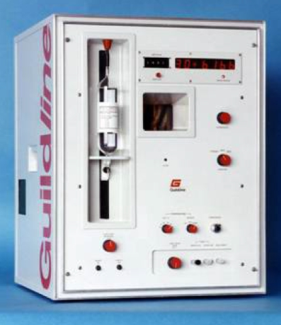
\includegraphics{E:/R/SOP/SOP_P04_Salinity_autosal8400/images/P04_image1_Guildline사의 Autosal 8400B.png}
\caption{Guildline사의 Autosal 8400B}
\end{figure}

\hypertarget{t-s-bridge}{%
\subsection{T-S bridge}\label{t-s-bridge}}

현장에서 온도와 전기전도도를 측정하여 염분을 계산하는 기기이지만 현재 해양에서 활용되지 않고 육상의 토양에서 염분을 측정하는 데 주로 이용된다. 아래 그림에 있는 장비는 5500 salinity bridge로 토양에서 연속으로 염분을 측정하는 장비로 전기전도도 범위가 2-40 mmho/cm이다. 해양에서는 T-S bridge를 사용하여 염분을 측정하는 경우가 거의 없으므로 이 기기에 대한 설명은 생략하겠다. 그리고 향후 해양환경공정시행법에서도 이 부분에 관한 내용은 삭제하는 것이 적절할 것으로 판단된다.
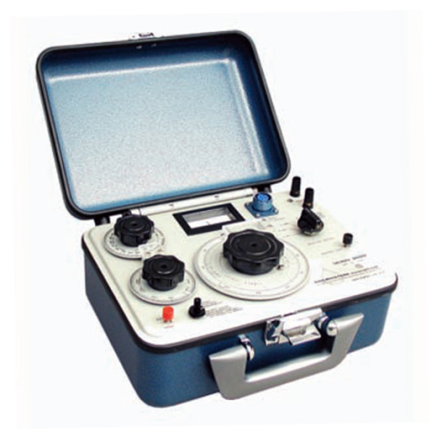
\includegraphics{E:/R/SOP/SOP_P04_Salinity_autosal8400/images/P04_image2_5500 salinity bridge.png}

\hypertarget{seabird-conductivity-sensor-sbe-4c}{%
\subsection{Seabird conductivity sensor (SBE 4C)}\label{seabird-conductivity-sensor-sbe-4c}}

SBE 4C 전기전도도 센서에 의한 전기전도도 측정은 30 cm\textsuperscript{3}/s로 일정하게 해수를 흐르게 하는 펌프로 해수를 직경 0.4 cm의 T-C duct로 유입되면서 수온이 즉시 감지되고 duct를 통해 해수가 흐르는 동안 0.73초 뒤에 전기전도도 셀로 해수가 들어간다. 펌프 속도가 일정하여서 항상 0.73초의 시간이 지연된다. 이 센서는 단독으로 운영되는 것이 아니라 주로 SBE 9plus data loger에 연결하여 사용한다.
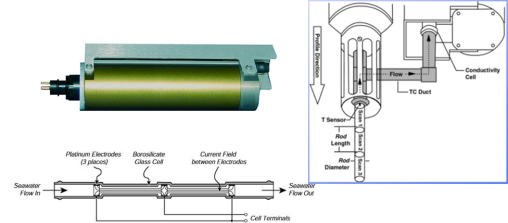
\includegraphics{E:/R/SOP/SOP_P04_Salinity_autosal8400/images/P04_image3_Seabird conductivity sensor.png}

\hypertarget{ysi-hydrolab-etc.-multiprobe-sensor}{%
\subsection{YSI, Hydrolab etc. multiprobe sensor}\label{ysi-hydrolab-etc.-multiprobe-sensor}}

아래 그림의 좌측은 YSI multiprobe이고 우측이 Hydrolab의 multiprobe이다. 이런 종류의 측정기에 사용되는 전기전도도 센서의 특징은 두 개의 전극이 부피를 알고 있는 공간에 설치되어 있고, 이 공간에 전기전도도 측정 대상 용액이 출입할 수 있는 구멍과 온도를 측정하는 센서가 함께 결합되어 있다. 두 전극에 전기를 연결하여 부피를 알고 있는 용액의 전기전도도와 온도를 측정하여 전극 사이의 전기전도도로 전환하여 염분을 계산한다.\\
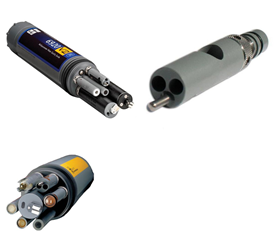
\includegraphics{E:/R/SOP/SOP_P04_Salinity_autosal8400/images/P04_image4_YSI multiprobe.png}\\
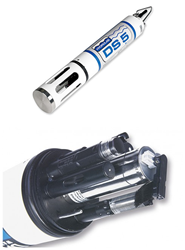
\includegraphics{E:/R/SOP/SOP_P04_Salinity_autosal8400/images/P04_image5_Hydrolab multiprobe.png}

4.5 각 기기들 간의 측정범위, 정밀도, 해상도는 아래의 표와 같다.

\hypertarget{uxc2dcuxb8ccuxcc44uxcde8-uxc804uxcc98uxb9ac-uxbcf4uxad00-uxae30uxb85d}{%
\section{시료채취, 전처리, 보관, 기록}\label{uxc2dcuxb8ccuxcc44uxcde8-uxc804uxcc98uxb9ac-uxbcf4uxad00-uxae30uxb85d}}

전기전도도를 이용해서 해수 염분을 측정하는 경우 채수기를 이용하여 해수시료를 채취하여 실험실에서 정밀염분측정기를 이용하여 염분을 측정하는 경우와 T-S bridge, CTD를 현장에서 운영하여 직접 전기전도도를 측정하여 함께 측정된 수온자료를 이용하여 염분으로 계산하는 경우가 있다. 해수시료의 염분을 실험실에서 측정하는 경우 시료채취, 전처리, 보관, 기록에 관한 사항을 다루고자 한다.

\hypertarget{uxc2dcuxb8ccuxcc44uxcde8-uxc6a9uxae30}{%
\subsection{시료채취 용기}\label{uxc2dcuxb8ccuxcc44uxcde8-uxc6a9uxae30}}

염분시료를 채취하기 위한 시료병은 해수와 유리의 화학적인 상호작용을 최소화하기 위해 경질유리(flint glass) 재질의 병을 사용하고, 증발 영향을 제거하기 위해 poly-seal screw cap을 사용한다. 최근 실험실 유리기구에 많이 사용되는 재질은 붕규산 유리 재질(borosilicate glass)**이다. 용기의 부피는 오염에 의한 영향을 최소화하기 위해 125-250 ml를 사용한다. 이러한 종류의 용기를 사용하면 염분 변화를 0.001이하로 6개월 정도 보관할 수 있다(Stalcup,1991). 시료병 뚜껑은 최소 2년 주기(최대 3년이내)로 교환을 해야 하며 염분병은 8년 주기 (최대 10년)로 교환한다.
*Pb 또는 K-SiO\textsubscript{2} 조성의 유리로 고굴절율과 빛의 산란이 높은 특징을 가지고 있어 렌즈, 광학기구, 프리즘, 장식용 유리로 상용됨
**붕소(Br)-SiO\textsubscript{2} 결합으로 구성된 유리로 물리, 화학, 온도에 따른 변화에 강하여 실험실, 부엌용기에 많이 사용된다. Pyrex, Boroil, Simax, Bomex등의 상표가 일반적이다.

\hypertarget{uxc2dcuxb8ccuxcc44uxcde8}{%
\subsection{시료채취}\label{uxc2dcuxb8ccuxcc44uxcde8}}

채수기로 채수한 해수시료 염분병 입구와 채수기의 출구 사이의 직접적인 접촉없이 염분병의 4분의 1정도를 채운 다음 뚜껑을 닫고 최소 10초 동안 흔든 후 비운다. 이러한 과정을 최소한 3회 반복한다. 해수시료를 시료병의 목부분까지 채운다음 병뚜껑을 해수시료로 잘 헹군 후 뚜껑을 닫는다. 시료를 채취할 때 표층수/빗물이 흘러들어가 오염되는 것을 주의한다.

\hypertarget{uxc2dcuxb8ccuxbcf4uxad00}{%
\subsection{시료보관}\label{uxc2dcuxb8ccuxbcf4uxad00}}

현장에서 염분을 측정할 때 시료 병을 보관 상자에 넣어서 염분 측정기가 있는 온도가 일정한 곳에 보관한다. 시료 병의 크기와 시료의 온도에 따라 수 시간 또는 하루 내에 실험실 온도와 평형이 이루어진다(Muller, 1999). 현장에서 분석이 어려우면 15-20 ℃로 보관할 경우 최대 10일간 보관할 수 있다(해양환경공정시행법, 2013). 시료를 보관할 때 병뚜껑과 목부분을 잘 닦아주어 병 뚜껑의 나사에 있는 물기가 건조되어 생긴 염에 의한 오염을 최소화한다.

\hypertarget{uxc2dcuxb8ccuxae30uxb85d}{%
\subsection{시료기록}\label{uxc2dcuxb8ccuxae30uxb85d}}

기록의 실수를 최대한 줄이기 위하여 시료병은 시료채취용 니스킨 병의 번호로 기록하기를 권장한다. 시료병을 명확히 구별하는 다른 방법을 사용할 수도 있다. 시료병에 필요한 정보는 cruise identification, station, cast number, water sampler number, storage case identification, salinity sample bottle number등이다.

\hypertarget{uxc5fcuxbd84uxce21uxc815}{%
\section{염분측정}\label{uxc5fcuxbd84uxce21uxc815}}

6.1 정밀염분측정기인 Autosal 8400B를 이용한 염분측정 방법에 대해서는 별도로 Autosal 측정방법에 자세히 설명한다.\\
6.2 Seabird 4C를 이용하여 현장에서 염분을 측정하기 전 온도가 조절되는 항온수조에 센서를 넣고 온도를 변화시키면서 전기전도도를 측정하고 이때 사용된 해수시료를 채취하여 실험실에서 Autosal 8400B를 이용하여 염분을 정밀하게 측정한다. 기기에서 측정된 주파수를 이용하여 교정식의 상수를 결정하고, 이 상수를 이용하여 측정주파수를 전기전도도로 환산한다. 온도와 전기전도도를 이용하여 염분값으로 전환한다. 교정 상수가 결정되면 현장에서 전기전도도와 온도를 동시에 측정하여 위의 식을 이용하여 자동으로 염분값을 환산할 수 있다. 교정수행은 교정에 사용되는 환경과 장비등을 기기 사용자가 구비하기 어렵고 제조사나 전문교정기관에서 주기적(1년마다)으로 실시할 것을 권장한다. 교정기관, 교정일자, 교정상수, 온도별 교정후 계산값과의 차이값을 자료와 함께 보고한다.\\
6.3 YSI, Hydrolab multiparameter conductivity sensor를 이용하여 염분을 측정하기 위해서 우선 센서교정을 실시한다. SBE 4C센서와 달리 센서교정은 센서교정용 용액을 이용하여 이용자가 직접 수행한다. 센서교정을 위한 기기조작에 대해서는 제조사의 장비 운영메뉴얼을 참고하여 조작한다. 기본적으로 이온을 포함한 용액의 전기전도도는 온도에 아주 민감하다(온도계수=3\%/℃). 교정 전에 온도센서가 정상적으로 작동하고 있는지 확인을 해야 하고, 전기전도도의 보고는 특정온도에서의 전기전도도 값으로 보고해야한다.(20.2 mS/cm at 14 ℃). 일반적인 전기전도도는 측정된 전기전도도 값의 온도보정이 되지않은 것이고 Specific Conductance는 측정된 전기전도도 값을 25 ℃일 때의 값으로 환산하여 보정한 값이다(온도보정계수=1.91\%=0.0191).
센서교정 절차는 다음과 같다.
- 전기전도도를 교정은 전기전도도를 알고 있는 적절한 용액을 선택한다(담수: 1.0 mS/cm, 하구역수: 10 mS/cm, 해수: 50 mS/cm).
- 교정시 센서에 공기방울이 있으면 액체의 부피변화로 인해서 전기전도도에 영향을 주기 때문에 공기방울을 잘 제거한다.
- 기기별 사용 메뉴얼의 교정절차에 따라 교정을 실시하고 교정용 전기전도도 측정 용액의 교정 전 전기전도도 값과 교정 후 전기전도도값을 측정온도와 함께 교정기록지에 기록한다.
- 탈이온수 또는 증류수를 사용하여 Low-End Specific Conductance Check을 수행하고 (5 μS/cm이하 전기전도도 용액 사용), 이러한 확인은 최소 1주일에 한 번씩 수행되어야 한다. 그리고 Low-End Specific Conductance Check수행에 사용된 용액의 전기전도도 값을 표시하고 측정된 전기전도도 값을 온도와 함께 교정기록지에 기록한다.
-최소 한 달에 한 번씩은 전기전도도센서 교정에 사용된 표준용액에 따라 500 또는 1000 μS/cm 용액으로 Mid-Range Specific Conductance Check를 수행해야 하고 사용된 용액의 전기전도도와 Mid-Range conductivity solution 측정된 전기전도도 값을 측정 온도와 함께 교정기록지에 기록해야한다. Mid-Range Specific Conductance Check는 선형성 시험이고 측정된 전기전도도 값과 용액에 표시된 전기전도도 값과의 차이는 10\% 이내이어야 한다.

\begin{figure}
\centering
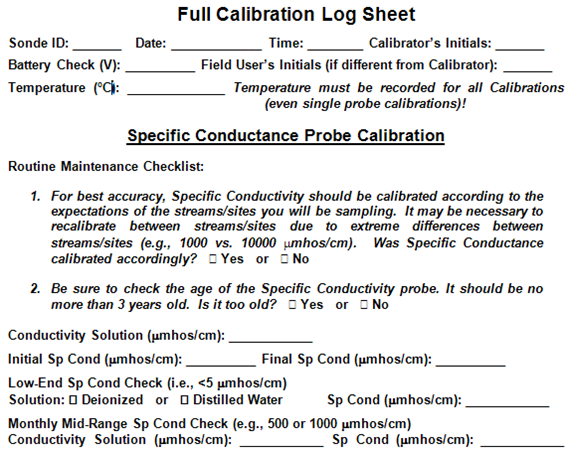
\includegraphics{E:/R/SOP/SOP_P04_Salinity_autosal8400/images/P04_image6_교정기록지.png}
\caption{교정기록지}
\end{figure}

\hypertarget{autosal-8400buxb97c-uxc774uxc6a9uxd55c-uxc5fcuxbd84uxce21uxc815uxbc29uxbc95}{%
\section{Autosal 8400B를 이용한 염분측정방법}\label{autosal-8400buxb97c-uxc774uxc6a9uxd55c-uxc5fcuxbd84uxce21uxc815uxbc29uxbc95}}

\hypertarget{uxac1cuxc694}{%
\subsection{개요}\label{uxac1cuxc694}}

AUTOSAL은 현장에서 채수한 샘플의 염분 값을 측정하는 장비로서 시료를 측정하기 앞서 AUTOSAL에 표준해수(standard seawater)로 초기화시킨 염분 표준정점과 시료의 상호비교 측정한 값을 전기전도도 비(conductivity ratio)로 지시하는 장비이다.

\hypertarget{uxc0acuxc591}{%
\subsection{사양}\label{uxc0acuxc591}}

(1)전원 : 교류 230V AC 또는 115V AC로 사용 가능하다\\
(2)Bath 용량 : 16.8 리터\\
(3)측정 지시값 : 2배의 전기전도도 비\\
(4)측정범위 : 0.005~42 psu (Conductivity=7.6 S/m 또는 Rt=1.15 에 해당한다)\\
(5)정확도 : ±0.002 psu\\
(6)분해능 : ±0.0002 psu\\
(7)Bath 온도 :\\
- setting temp : 18℃, 21℃, 24℃, 27℃, 30℃, 33℃
- 정확도 : ±0.02 ℃
- 안정도 : ±0.001 ℃/day
(8)Scale Suppression : 0~2.2 Conductivity ratio (22 스텝)

\begin{figure}
\centering
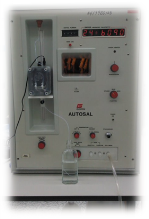
\includegraphics{E:/R/SOP/SOP_P04_Salinity_autosal8400/images/P04_image7_AUTOSAL 8400B.png}
\caption{UTOSAL(8400B)}
\end{figure}

\begin{figure}
\centering
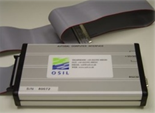
\includegraphics{E:/R/SOP/SOP_P04_Salinity_autosal8400/images/P04_image8_computer interface.png}
\caption{computer interface}
\end{figure}

\begin{figure}
\centering
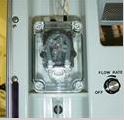
\includegraphics{E:/R/SOP/SOP_P04_Salinity_autosal8400/images/P04_image9_외부펌프.png}
\caption{외부펌프}
\end{figure}

\begin{figure}
\centering
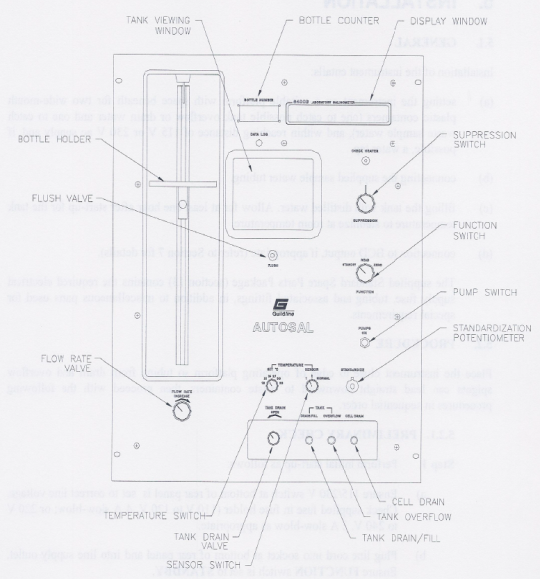
\includegraphics{E:/R/SOP/SOP_P04_Salinity_autosal8400/images/P04_image10_Autosal Front Panel.png}
\caption{Autosal Front Panel}
\end{figure}

\hypertarget{uxc900uxbe44uxbb3c}{%
\subsection{준비물}\label{uxc900uxbe44uxbb3c}}

표준해수, 증류수, 위생장갑, 킴와이프, 샘플병, 전기테이프, 기록장, 바스켓(폐액통)

\hypertarget{autosaluxc744-uxc791uxb3d9uxc2dcuxd0a4uxae30-uxc804-uxc810uxac80uxd560-uxc0acuxd56d}{%
\subsection{Autosal을 작동시키기 전 점검할 사항}\label{autosaluxc744-uxc791uxb3d9uxc2dcuxd0a4uxae30-uxc804-uxc810uxac80uxd560-uxc0acuxd56d}}

(1)가능하다면 출입문을 모두 닫는다.\\
(2)각 switch 및 valve 위치를 확인한다.\\
- suppression switch : 맨 왼쪽으로 다 돌린 상태(증류수로 셀 세척하고 확인한 상태)\\
- function switch : standby 위치\\
- pump switch : off 위치\\
- flow rate valve : 최대로 열린 상태(외장펌프를 이용할 경우)\\
- temperature set switch : 전에 setting 한 값에 위치\\
- temperature sensor switch : normal 위치\\
- tank drain valve : 최대로 닫힌 상태\\
(3)tank drain/fill, tank overflow : 현재 상태 그대로(호스가 연결되지 않은 상태)\\
(4)샘플 공급용 테프론 튜브를 증류수병에 연결한다.\\
(5)cell drain과 연결된 호스가 폐통에 모인 물에 잠기지 않도록 길이를 조정한다. cell drain에서 나오는 물이 물통에 떨어지도록 조절하고 그렇지 않으면 염분 측정값이 튀어서 측정 결과의 신뢰성 저하를 초래한다.\\
(6)실내 온도로 항온을 유지하기 위해 표준해수, 샘플병, 증류수, 위생장갑 등 실험물품을 Autosal 근처 테이블에 미리 비치한다.\\
(7)실내 온도를 관찰할 수 있는 온도계를 비치한다.

\hypertarget{autosaluxc744-uxc791uxb3d9uxc2dcuxd0ac-uxb54c-uxc810uxac80uxd560-uxc0acuxd56d}{%
\subsection{Autosal을 작동시킬 때 점검할 사항}\label{autosaluxc744-uxc791uxb3d9uxc2dcuxd0ac-uxb54c-uxc810uxac80uxd560-uxc0acuxd56d}}

AUTOSAL은 사용하기 최소 8시간 전에 전원을 켜 둔다.
(1) AC 전원\\
- 플러그를 콘센트에 꽂는다.
- Autosal과 computer interface는 연결된 상태인지 확인한다.
- 외부펌프의 연결 상태를 확인한다.
- AUTOSAL 전원을 켠다(전원 스위치는 AUTOSAL 후면 아래에 위치한다).
- 전원이 들어오지 않으면 FUSE(250V / 2A)를 확인 후 교체한다.
- 후면에 위치한 냉각 팬이 돌아가는지 확인한다.
(2)temperature bath\\
- 수조를 볼 수 있는 창을 통해서 수조내에 물(증류수)이 차 있는지 확인한 후 부족하거나 없다면 보충한다.\\
- 램프를 확인한다. 램프 불이 들어오지 않으면 수조를 들여다 볼 수 있는 창을 통해서 전기전도도 셀 내 코일이 보이지 않는다.\\
- 실내 온도에 따라 온도 설정 스위치를 이용하여 bath 온도를 조절한다. bath의 설정온도는 실내 온도의 --2℃~+4℃ 이내에 있도록 한다.
(3)temperature sensor\\
- temperature sensor switch를 normal로 설정하고 temperature set switch를 33으로 조절한다(heater lamp가 on-정상).\\
- temperature sensor switch를 normal로 설정하고 temperature set switch를 18로 조절한다(heater lamp가 off-정상).\\
(4)temperature sensor check\\
- bath 온도를 설정하고 약 1시간 정도 경과 후, heater lamp가 주기적으로 꺼지고 켜짐을 반복한다.\\
- temperature sensor switch를 normal에서 1로 조절하고 약 4~5분 이내 heater lamp가 주기적으로 꺼지고 켜짐을 반복한다.
- temperature sensor switch를 1에서 2로 조절하고 약 4~5분 이내 heater lamp가 주기적으로 꺼지고 켜짐을 반복한다.\\
- temperature sensor switch를 원래 normal로 설정한다.\\
- heater lamp가 주기적으로 꺼지고 켜지지 않고 계속 꺼진 상태라면 heater lamp가 고장 난 것이다(새 heater lamp로 교체 요망).

\hypertarget{uxd45cuxc2dcuxd654uxba74uxc758-uxc9c0uxc2dcuxac12uxc744-uxc77duxb294-uxbc29uxbc95}{%
\subsection{표시화면의 지시값을 읽는 방법}\label{uxd45cuxc2dcuxd654uxba74uxc758-uxc9c0uxc2dcuxac12uxc744-uxc77duxb294-uxbc29uxbc95}}

(1)function switch, standby 상태\\
temperature set switch가 24℃인 경우\\
(2)function switch, read 상태\\
suppression switch 1.9 위치한 경우\\
suppression switch 2.0 위치한 경우\\
computer interface 연결한 상태에서는 -- 값을 읽지 못한다.

\hypertarget{autosal-uxd45cuxc900uxd654-uxbc0f-uxc2dcuxb8ccuxce21uxc815-uxc804-uxc608uxc5f4warming-up}{%
\subsection{Autosal 표준화 및 시료측정 전 예열(warming-up)}\label{autosal-uxd45cuxc900uxd654-uxbc0f-uxc2dcuxb8ccuxce21uxc815-uxc804-uxc608uxc5f4warming-up}}

기록장에 측정일자, Autosal on 시간, off 시간, Bottle Number, zero 값 기록\\
(1)컴퓨터에서 Salinometer Data Logger 실행\\
(2)File → New. Serial Number 입력 후 확인

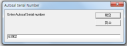
\includegraphics{E:/R/SOP/SOP_P04_Salinity_autosal8400/images/P04_image11_New Serial Number 입력창.png}

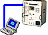
\includegraphics{E:/R/SOP/SOP_P04_Salinity_autosal8400/images/P04_image12_컴퓨터와 Autosal 연결상태.png}

\begin{enumerate}
\def\labelenumi{(\arabic{enumi})}
\setcounter{enumi}{2}
\tightlist
\item
  Run ID와 File Name 입력 후 OK
\end{enumerate}

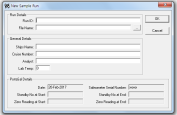
\includegraphics{E:/R/SOP/SOP_P04_Salinity_autosal8400/images/P04_image13_Run ID와 File Name 입력창.png}

(4)이 문구가 나오면 Autosal의 Function Switch를 Zero로 놓고 값을 확인한다. 0.0+000x : x=±5 이하면 정상, 그렇지 않으면 전자회로를 조정해야 한다.

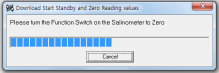
\includegraphics{E:/R/SOP/SOP_P04_Salinity_autosal8400/images/P04_image14_진행 중 안내창.png}

(5)Autosal의 Function Switch를 Standby로 돌리고 확인한다.

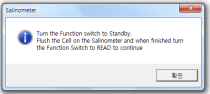
\includegraphics{E:/R/SOP/SOP_P04_Salinity_autosal8400/images/P04_image15_확인창.png}

(6)셀을 증류수로 6회 정도 세척한다.\\
- 테프론 튜브의 오염 방지를 위하여 킴와이프로 닦아준 후 증류수 병에 담근다.\\
- Autosal의 Pump Switch를 켜고 구멍을 3초 정도 막아 Flushing하여 마지막 실험에 전기전도도 셀 안에 채워 두었던 증류수를 제거 한 후 Pump Switch를 끈다.\\
- 외장 Pump(flow rate : 1)의 Switch를 이용하여 전기전도도 셀 안에 증류수가 다 채워지면 외장 Pump의 Switch를 끈다.\\
- 위의 과정을 6회 정도 반복하여 세척한 후 증류수를 전기전도도 셀에 채워 Function Switch를 Standby에서 Read로 돌리고 10초 기다리는 동안에 Suppression Switch를 돌려 맞춘다. 측정범위를 벗어나면 display 지시 값이 깜박거린다 → 증류수 Suppression Switch 0.0 → Autosal의 display 지시 값을 기록장에 적어 놓는다(증류수는 깨끗하여 Autosal 측정 불가).\\
- Function Switch를 Read에서 Standby로 돌린다.\\
(7)해수로 전기전도도 셀을 20분 이상 충분히 적셔준다. 전기전도도 코일을 해수로 충분히 적셔 시료를 측정하기 위한 최적의 상태로 만들어 준다.

\begin{figure}
\centering
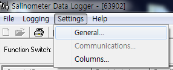
\includegraphics{E:/R/SOP/SOP_P04_Salinity_autosal8400/images/P04_image16_Settings 메뉴 General 탭.png}
\caption{캡션}
\end{figure}

\begin{figure}
\centering
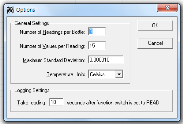
\includegraphics{E:/R/SOP/SOP_P04_Salinity_autosal8400/images/P04_image17.png}
\caption{캡션}
\end{figure}

\begin{itemize}
\tightlist
\item
  테프론 튜브를 킴와이프로 닦아주고 해수(전에 쓰고 남은 표준해수 또는 해수)를 pump를 이용하여 셀 안에 채운 후 flushing한다. 이 세척 과정을 3\textasciitilde4회 반복 후 전기전도도 셀에 해수를 채워 Function Switch를 Read로 돌리고 10초 기다리는 동안에 Suppression Switch를 돌려 맞춘다. 측정범위를 벗어나면 display 지시 값이 깜박거린다. → 표준해수 Sal. 35는 Suppression Switch 1.9 → 20분 셀을 적신다.\\
\item
  1200초 동안 Reading이 끝나면 Function Switch를 Read에서 Standby로 돌린다.\\
\item
  만약 Maximum Standard Deviation이 0.000010이 넘어가면 아래의 화면이 나타난다. 마우스로 대략 중간값을 클릭하고 Accept Reading 클릭
\end{itemize}

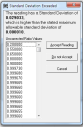
\includegraphics{E:/R/SOP/SOP_P04_Salinity_autosal8400/images/P04_image18.png}
위의 화면이 뜨지 않으면 Autosal이 충분히 안정된 상태이다.

\begin{figure}
\centering
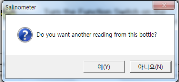
\includegraphics{E:/R/SOP/SOP_P04_Salinity_autosal8400/images/P04_image19.png}
\caption{캡션}
\end{figure}

아니요를 클릭한다.

\begin{figure}
\centering
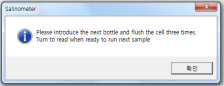
\includegraphics{E:/R/SOP/SOP_P04_Salinity_autosal8400/images/P04_image20_확인창.png}
\caption{캡션}
\end{figure}

확인을 클릭한다.

\begin{figure}
\centering
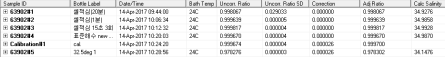
\includegraphics{E:/R/SOP/SOP_P04_Salinity_autosal8400/images/P04_image21_Bottle Label 입력 화면.png}
\caption{캡션}
\end{figure}

\begin{itemize}
\tightlist
\item
  마우스 오른쪽 버튼을 클릭 후 Bottle Label을 적을 수 있다.\\
\item
  예를 들어 63902\#3 화면에 보이는 값은 3회 측정값의 평균이다.\\
  를 클릭하면 각 1회씩(15초)의 평균값이 나오고 그 밑을 다시 한번 클릭하면 1초간의 데이터를 확인할 수 있다.\\
  (8)남은 표준해수(다시 섞어줌)로 3회 15초간 적셔준다.
\end{itemize}

\begin{figure}
\centering
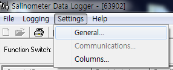
\includegraphics{E:/R/SOP/SOP_P04_Salinity_autosal8400/images/P04_image22_Settings 메뉴 General 탭.png}
\caption{캡션}
\end{figure}

\begin{figure}
\centering
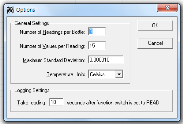
\includegraphics{E:/R/SOP/SOP_P04_Salinity_autosal8400/images/P04_image23.png}
\caption{캡션}
\end{figure}

\begin{itemize}
\tightlist
\item
  3회의 display 지시 값의 끝자리 숫자가 ±5 이상 변동이 없을 때까지 반복 측정한다.
\end{itemize}

\hypertarget{autosal-uxd45cuxc900uxd654standardization-potentiometer-uxc774uxc6a9}{%
\subsection{Autosal 표준화(standardization potentiometer 이용)}\label{autosal-uxd45cuxc900uxd654standardization-potentiometer-uxc774uxc6a9}}

Autosal Warming-up 종료 후 표준화할 수 있다.\\
(1)새 표준해수를 잘 섞어준 후 오픈하여 테프론 튜브를 킴와이프로 닦아 표준해수병에 담근다.\\
(2)Autosal의 Pump Switch를 켜고 구멍을 3초 정도 막아 Flushing하여 마지막 실험에 전기전도도 셀 안에 채워 두었던 해수를 제거한 후 Pump Switch를 끈다.\\
(3)외장 Pump(flow rate : 1)의 Switch를 이용하여 전기전도도 셀 안에 표준해수가 다 채워지면 외장 Pump의 Switch를 끈다.\\
(4)위의 세척 과정을 3\textasciitilde4회 정도 반복 후 표준해수를 전기전도도 셀에 채운다.\\
(5)Function Switch를 Read로 돌리고 10초 기다리는 동안 Standardization Potentiometer의 고정핀을 풀어(고정핀을 위로 올린다), Potentiometer를 돌려 표준해수병의 종이 상표에 있는 K15값의 2배로 맞추고 고정핀을 잠근다(고정핀을 밑으로 내린다).\\
예를 들어 K15 = 0.99996이면, 0.99996 × 2 = 1.99992로 맞춘다.\\
따라서, 1.99992 값이 display에 지시되도록 Potentiometer를 돌린다.\\
(6)30초 동안 Reading이 끝나면 Function Switch를 Read에서 Standby로 돌린다.\\
(7)display 지시 값이 표준해수 K15값의 2배와 비슷한 값이 3번(매회 셀 안을 flushing한 후 새로 셀을 채운다)정도 나올 때 까지 (5)\textasciitilde(6)과정을 반복한다.\\
이때의 4자리 디지트가 표준화한 상수이며 Bottle Counter에 넣어주고 기록장에도 기록한다. 표준화 상수 끝자리 숫자가 ±5 이상 변동되면 Autosal을 다시 표준화한다.

\hypertarget{autosal-uxd45cuxc900uxd654-uxc808uxcc28uxd504uxb85cuxadf8uxb7a8-uxc774uxc6a9}{%
\subsection{Autosal 표준화 절차(프로그램 이용)}\label{autosal-uxd45cuxc900uxd654-uxc808uxcc28uxd504uxb85cuxadf8uxb7a8-uxc774uxc6a9}}

Standardization potentiometer 이용하여 표준화를 한 후 Autosal 및 표준해수 변화 추이를 간편하게 표준화 할 수 있다.\\
Autosal Warming-up 종료 후 표준화 할 수 있다.\\
(1)새 표준해수를 잘 섞어준 후 열고 테프론 튜브를 킴와이프로 닦아 표준해수병에 담근다.
(2)Autosal의 Pump Switch를 켜고 구멍을 3초 정도 막아 Flushing하여 마지막 실험에 전기전도도 셀 안에 채워 두었던 해수를 제거한 후 Pump Switch를 끈다.\\
(3)외장 Pump(flow rate : 1)의 Switch를 이용하여 전기전도도 셀 안에 표준해수가 다 채워지면 외장 Pump의 Switch를 끈다.\\
(4)위의 세척을 3\textasciitilde4회 정도 반복한 후 표준해수를 전기전도도 셀에 채운다.\\
(5)Function Switch를 Read로 돌리고 10초 기다리는 동안에 Suppression Switch를 돌려 맞춘다(측정범위를 벗어나면 display 지시 값이 깜박거린다 → 표준해수 Sal. 35는 Suppression Switch 1.9) → Reading이 끝나면 Function Switch를 Read에서 Standby로 돌린다 → 앞의 과정을 3회(매회 셀 안을 flushing 한 후 새로 셀을 채움) 반복 측정\\
(6)셀 안에 남아 있는 표준해수를 flushing 한 후 전기전도도 셀에 표준해수를 다시 채운다.

\begin{figure}
\centering
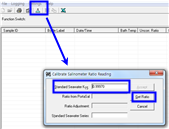
\includegraphics{E:/R/SOP/SOP_P04_Salinity_autosal8400/images/P04_image24_표준해수병 K15값 입력.png}
\caption{캡션}
\end{figure}

\begin{itemize}
\tightlist
\item
  파란 네모칸의 삼각플라스크병 모양을 누른다.\\
\item
  Standard Seawater K15 칸에 오픈한 표준21해수병의 종이 상표에 있는 K15값을 입력한다.\\
\item
  Get Ratio 클릭 후 Function Switch를 Read로 돌리고 10초 기다리는 동안에 Suppression Switch를 돌려 맞춘다(측정범위가 벗어나면 display 지시 값이 깜박거린다 → 표준해수 Sal. 35는 Suppression Switch 1.9).\\
\item
  Reading이 끝나면 Function Switch를 Read에서 Standby로 돌린다.\\
\item
  Autosal display 지시 값이 위에 측정한 값과 비슷하게 나오면 Accept를 누른다.\\
\item
  아래 화면처럼 보정값 Ratio 및 Salinity 값이 적용되어 나온다.
\end{itemize}

\begin{figure}
\centering
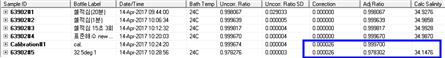
\includegraphics{E:/R/SOP/SOP_P04_Salinity_autosal8400/images/P04_image25_Ratio 및 Salinity 값 확인.png}
\caption{캡션}
\end{figure}

\hypertarget{uxd574uxc218-uxc2dcuxb8cc-uxc5fcuxbd84uxce21uxc815-uxc808uxcc28}{%
\subsection{해수 시료 염분측정 절차}\label{uxd574uxc218-uxc2dcuxb8cc-uxc5fcuxbd84uxce21uxc815-uxc808uxcc28}}

(1)해수 시료를 잘 섞어준 후 열고 테프론 튜브를 킴와이프로 닦아 해수 시료병에 담근다.\\
(2)Autosal의 Pump Switch를 켜고 구멍을 3초 정도 막아 Flushing하여 마지막 실험에 전기전도도 셀 안에 채워 두었던 해수를 제거한 후 Pump Switch를 끈다.\\
(3)외장 Pump(flow rate : 1)의 Switch를 이용하여 전기전도도 셀 안에 해수 시료가 다 채워지면 외장 Pump의 Switch를 끈다.\\
(4)위의 세척을 3\textasciitilde4회 정도 반복한 후 해수 시료를 전기전도도 셀에 채운다.\\
(5)Function Switch를 Read로 돌리고 10초 기다리는 동안에 Suppression Switch를 돌려 맞춘다(측정범위가 벗어나면 display 지시 값이 깜박거린다) → Reading이 끝나면 Function Switch를 Read에서 Standby로 돌린다 → 앞의 과정을 3회(매회 셀 안을 flushing 한 후 새로 셀을 채운다) 반복 측정한다.

\hypertarget{autosal-uxb044uxae30}{%
\subsection{Autosal 끄기}\label{autosal-uxb044uxae30}}

(1)증류수로 전기전도도 셀을 반복 세척(6회 정도)하고 셀 안에 증류수를 채운다.\\
(2)Function Switch를 Standby에서 Read로 돌리고 10초 기다리는 동안에 Suppression Switch를 돌려 맞춘다(측정범위가 벗어나면 display 지시 값이 깜박거린다 → 증류수 Suppression Switch 0.0 → Autosal의 display 지시 값을 기록장에 적어 놓는다(증류수는 깨끗하여 Autosal 측정 불가).\\
(3)Function Switch를 Read에서 Standby로 돌린다.

\begin{figure}
\centering
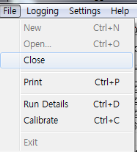
\includegraphics{E:/R/SOP/SOP_P04_Salinity_autosal8400/images/P04_image26_File 메뉴 Close 탭.png}
\caption{캡션}
\end{figure}

(4)File → Close 선택한다.

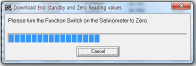
\includegraphics{E:/R/SOP/SOP_P04_Salinity_autosal8400/images/P04_image27_진행 중 안내창.png}\\
(5)Function Switch를 Standby에서 Zero로 돌리고 Zero 값 확인 후 기록장에 기록한다.\\
(6)Function Switch를 Zero에서 Standby로 돌린다.\\
(7)AUTOSAL 전원 스위치를 끈다(전원 스위치는 AUTOSAL 후면 아래에 위치).\\
(8)AUTOSAL 사용이 끝난 후 각 소모품 등은 원래 자리에 비치한다.

\hypertarget{autosal-uxc804uxae30uxc804uxb3c4uxb3c4-uxc140-uxc138uxcc99-uxbc0f-uxacf5uxae30uxbc29uxc6b8-uxc81cuxac70-uxbc29uxbc95}{%
\subsection{Autosal 전기전도도 셀 세척 및 공기방울 제거 방법}\label{autosal-uxc804uxae30uxc804uxb3c4uxb3c4-uxc140-uxc138uxcc99-uxbc0f-uxacf5uxae30uxbc29uxc6b8-uxc81cuxac70-uxbc29uxbc95}}

(1)OSIL 세척 방법\\
- 20mL 증류수에 10mL Decon 90을 섞은 후 methanol(95\% 이상) 170mL를 넣는다. methanol은 독성과 발화성 물질로 사용 시 후드에서 사용하기를 권장한다.\\
- 세척액을 전기전도도 셀에 채우고 flushing을 하여 3\textasciitilde4회 반복한 후 셀을 다시 채워 대략 20분 정도 둔다.\\
- 전기전도도 셀 안에 남아 있는 세척액을 모두 flushing(대략 10초) 한다.\\
- 400mL 증류수로 전기전도도 셀을 채우고 flushing을 반복하여 세척한다.\\
- drain된 물은 따로 폐기물 통에 모아서 버린다.\\
- 공기방울 제거 후 전기전도도 셀을 남은 표준해수로 충분히 적신 후 시료를 측정한다.\\
(2)Guildline 방법\\
- CLR, Isopropyl Alcohol, 증류수를 각각 200mL 정도 준비한다.\\
- CLR로 전기전도도 셀을 채우고 flushing을 하여 3\textasciitilde4회 반복한 후 셀을 다시 채워 대략 20분간 둔다.\\
- 전기전도도 셀 안에 남아 있는 CLR를 모두 flushing(대략 10초) 한다.\\
- Isopropyl Alcohol를 전기전도도 셀에 채우고 flushing을 하여 5\textasciitilde7회 반복한 후 셀을 다시 채워 10\textasciitilde15분 정도 둔다.\\
- 전기전도도 셀 안에 남아 있는 Isopropyl Alcohol를 모두 flushing(대략 10초) 한다.\\
- 400mL 증류수로 전기전도도 셀을 채우고 flushing을 반복하여 세척한다.\\
- drain된 물은 따로 폐기물 통에 모아서 버린다.\\
- 공기방울 제거 후 전기전도도 셀을 남은 표준해수로 충분히 적신 후 시료를 측정한다.

\hypertarget{uxc8fcuxc758uxc0acuxd56d}{%
\subsection{주의사항}\label{uxc8fcuxc758uxc0acuxd56d}}

(1)표준해수 및 시료는 측정하기 전 뚜껑 쪽을 손가락으로 잡고 손목을 이용해 위·아래로 돌려주면서 고루 섞어준다. 섞은 후 작은 기포까지 사라졌을 때 전기전도도 셀에 표준해수 및 시료를 채운다. 시료에 부유물질이 있으면 전기전도도 셀의 코일에 부유물질이 끼지 않도록 가라앉힌 후 사용한다. 부유물질이 있는 해수를 여과하면 염분 측정값에 변화가 있는 것을 관찰할 수 있다.\\
(2)cell drain과 연결된 호스가 폐통에 모인 물에 잠기지 않도록 길이를 조정한다. cell drain에서 나오는 물이 물통에 떨어지도록 조절하고 그렇지 않으면 염분 측정값이 튀어서 측정 결과의 신뢰성 저하된다.\\
(3)전기전도도 셀 안에 공기방울이 생겼을 경우 공기방울을 제거하고 측정한다. 공기방울 1\textasciitilde2개 정도는 전체 평균값에는 크게 차이를 일으키지 않지만, 마지막 digit값을 변화시킨다. flushing하여 제거할 수 있다.\\
- 작은 공기방울이 많이 끼였을 경우 flushing으로 제거가 되지 않아 전기전도도 셀 세척 및 공기방울 제거 방법으로 제거할 수 있다. 대략 0.001psu 정도의 차이를 일으킨다.\\
(4)외장펌프에 공기방울이 있을 시 셀 유입이 느려질 수 있다. 외장펌프의 뚜껑을 열어 공기방울이 낀 튜빙 쪽을 손가락으로 눌러주거나 쳐서 공기방울을 제거한다.\\
(5)셀 내부로 시료가 들어가지 않을 때 Autosal 전면부에 있는 4개의 나사를 풀고 조심스럽게 당겨서(증류수가 들어있는 bath도 같이 레일을 타고 바깥으로 나오므로 앞으로 쏠리지 않도록 주의) 각 호스의 연결이 제대로 되어 있는지, impeller 벨트(O ring)가 연결되었는지를 확인하여 조치한다.\\
(6)30분 이상 자리를 비우고 다시 Autosal을 측정할 때 남은 표준해수 또는 해수로 3회\textasciitilde6회 정도 반복 분석한 후 결과가 비슷하게 나오는지 확인하고 시료를 측정한다.
(7)약 4\textasciitilde5시간 자리를 비울 때 증류수로 셀을 세척하고 셀 안에 증류수를 채워놓는다. 그 후 시료를 다시 측정 시 해수로 반복 분석하여 비슷한 값이 나올 때 값을 측정한다.\\
(8)표준화시 적은 양의 남은 표준해수(초기 부피의 15\% 미만)를 사용하지 않는다. 염 농도가 높아져 2ppm 이상의 오류가 발생할 수 있다. 사용한 표준해수는 시간이 지날수록 공기와의 접촉으로 인해 염 농도가 높아진다.\\
(9)display의 마지막 ±1 digit 차이는 대략 0.0002psu에 해당한다(35psu일 때).\\
(10)bath temperature ±0.5 mK 차이는 ±2 digits에 해당한다.

\hypertarget{uxcc38uxace0uxbb38uxd5cc-3}{%
\section{참고문헌}\label{uxcc38uxace0uxbb38uxd5cc-3}}

Cox, R.A., Culkin, F., Riley, J.P. (1967) The electrical conductivity/chlorinity relationship in natural sea water. Deep-Sea Research, 14:203-220
Saunders, P.M. (1990) The international temperature scale of 1990, ITS-90. WOCE Newsl. No.~10
Stalcup, M.C.(1991) Salinity measurements. WHP Operations and Methods
Muller, T.J. (1999) Determination of salinity. In Methods of Seawater Analysis. Eds Grasshoff, K., Kremling, K., Ehrhardt, M. Wiley-VCH
해양환경공정시험기준 (2013) 해양수산부고시 제2013-230호

\hypertarget{uxd654uxd559uxc801-uxc0b0uxc18cuxc694uxad6cuxb7c9-uxbd84uxc11d-uxd45cuxc900uxc6b4uxc601uxc808uxcc28uxc11c}{%
\chapter{화학적 산소요구량 분석 표준운영절차서}\label{uxd654uxd559uxc801-uxc0b0uxc18cuxc694uxad6cuxb7c9-uxbd84uxc11d-uxd45cuxc900uxc6b4uxc601uxc808uxcc28uxc11c}}

\hypertarget{uxbaa9uxc801-uxbc0f-uxbc94uxc704-2}{%
\section{목적 및 범위}\label{uxbaa9uxc801-uxbc0f-uxbc94uxc704-2}}

화학적 산소요구량은 해수시료를 알카리성으로 하여 산화제인 과망간산칼륨을 일정량 넣은 다음 60분간 중탕 가열반응 시켜 화학적으로 산화시킬수 있는 물질을 산화시킬 때 소비되는 과망간산칼륨의 양으로부터 산소량을 유추하여 해수 시료 중 유기물의 양을 간접적으로 표현한다. 이 표준운영절차서는 해양수산부의 해양환경공정시행법 (2013-230)에서 반응시 Grahm 응축기를 부착한 250ml Erlenmeyer Flask를 대신하여 Borosilicate Watch Glass와 100ml Borosilicate 비이커를 반응용기로 사용하여 많은 수의 시료를 동시에 분석할 수 있는 장점을 가지고 있다. 한국해양과학기술원에서 변형한 방법(KIOST modified MOF 2013-203)에 대한 내용을 중심으로 측정원리, 분석준비, 분석과정 및 분석 후 자료처리 등을 포함한다.

\hypertarget{uxce21uxc815uxc6d0uxb9ac-1}{%
\section{측정원리}\label{uxce21uxc815uxc6d0uxb9ac-1}}

해수시료를 알칼리성으로 하여 산화제인 과망간산칼륨을 일정량 과량으로 넣은 다음 60분간 가열 반응시켜 화학적으로 산화시킬 수 있는 물질을 산화시키며, 이때 소비되는 과망간산칼륨의 양으로부터 산소량을 유추하는 것으로 해수 시료 중 유기물의 양을 간접적으로 표현할 수 있다.

\begin{figure}
\centering
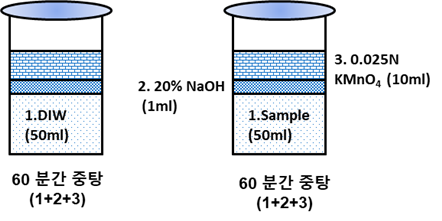
\includegraphics{E:/R/SOP/SOP_C06_COD/images/C06_image1_중탕 가열반응 과정.png}
\caption{캡션을 입력하세요}
\end{figure}

단계별로 살펴보면 먼저 과망간산칼륨용액을 첨가한 후 가열하여 유기물을 산화시킨다(①식). 이 때 반응하고 남은 요오드화칼륨용액은 황산용액과 함께 첨가된 요오드이온(I\textsuperscript{-})을 아이오딘(I\textsubscript{2})으로 산화시킨다(②식). 형성된 아이오딘(I\textsubscript{2})은 과잉의 요오드이온(I\textsuperscript{-})과 반응하여 트리아이오다이드 착물(I\textsuperscript{3-})을 형성한다(③식). 이 때 유리된 트리아이오다이드 착물(I\textsuperscript{3-}))은 첨가되어진 티오황산나트륨에 의해 다시 요오드이온(I\textsuperscript{-}))으로 환원된다(④식). 이 때 트리아이오다이드 착물(I\textsuperscript{3-}))은 티오황산나트륨에 의해 완전히 환원되기 전 넣어준 녹말지시약과 반응하여 푸른색을 띈다(⑤식). 그러므로 푸른색이 사라질 때까지 첨가되어진 티오황산나트륨의 양으로부터 과잉으로 남은 과망간산칼륨의 양을 알 수 있다.

\begin{enumerate}
\def\labelenumi{(\arabic{enumi})}
\tightlist
\item
  \(8{MnO_{4}}^{-} +\) 유기물 \(→ 8MnO +8OH^{-} + 6CO_{2} +2H_{2}O\)\\
\item
  \({MnO_{4}}^{-} + 2I^{-} + 8H^{+} → Mn^{2+} + I_{2} + 4H_{2}O\)\\
\item
  \(I_{2} +I^{-} = I^{3-}\)\\
\item
  \(I^{3-} +2{S_{2}O_{3}}^{2-} → 3I^{-} +{S_{4}O_{6}}^{2-}\)\\
\item
  녹말 + \(I^{3-}\) → 푸른색
\end{enumerate}

유기물이 없는 바탕용액(초순수수)에서 동일한 실험을 수행하여 사용된 시약등에 의해 소비되는 과망간산카륨을 제외하여 순수하게 시료에 포함된 유기물을 산화하는데 사용되어진 과망간산칼륨의 양을 계산한다. 위 반응식에서 유기물을 분해하는데 소비되어진 과망간산칼륨의 양은 바로 같은 유기물을 분해하는데 요구되어지는 산소의 양과 같으므로 이를 화학적산소요구량(Biochemical Oxygen Demand)이라고 하며, 이 반응에 참여한 과망간산칼륨의 당량은 산소의 당량과 같으므로 이 관계식으로부터 화학적산소요구량을 계산할 수 있다.
이 방법의 정량범위는 0.18\textasciitilde8 mgO\textsubscript{2}/L 이고, 95\% 신뢰도(k=2) 수준에서 검출한계(MDL)는 0.18 mgO2/L 이고 불확도는 0.11 mgO\textsubscript{2}/L이다. 60분간 가열하였을 때 최초에 첨가한 과망간산칼륨용액의 약 1/2이 잔존할 수 있는 양을 시료의 양으로 한다. 단 알칼리성 과망간산칼륨법에 의한 산소요구량이 8 mg O\textsubscript{2}/L 이하인 경우에는 시료양을 50 mL로 한다.

\hypertarget{uxbc29uxd574uxbb3c-1}{%
\section{방해물}\label{uxbc29uxd574uxbb3c-1}}

유기물의 난분해성 정도와 염분 등의 간섭조건에 따라 산화정도 차이가 크다. 자연시료를 측정할 경우 총 유기탄소 측정에 근거한 이론적산소요구량을 기준으로 대체로 30~50\%의 산화효율을 보이고 있어 해수시료중의 유기물 농도의 간접적인 지표로 이용하기에 신뢰성이 낮다. 중크롬산칼륨은 과망간산칼륨보다 강력한 산화제로서 상대적으로 산화효율은 높으나 해수시료의 경우 염소계 이온에 의한 간섭효과가 큰 문제점이 있다.

\hypertarget{uxae30uxad6c-uxbc0f-uxae30uxae30-1}{%
\section{기구 및 기기}\label{uxae30uxad6c-uxbc0f-uxae30uxae30-1}}

해수중 화학적 산소요구량 분석에는 필요한 기구 및 기기는 반응용기(4.1), 항온수조(4.2), 시계접시(4.3), 피펫류(4.4), 적정용 자동뷰렛(4.5)등이 있다. 실험에 사용되는 초자류를 10\%의 염산으로 세척한 후 초순수수로 3회 헹구어 사용한다. 분석기기의 구성과 사용법은 부록에서 자세하게 다루고자 한다.

\hypertarget{uxbc18uxc751uxc6a9uxae30}{%
\subsection{반응용기}\label{uxbc18uxc751uxc6a9uxae30}}

반응용기로 용액을 부을 때 사용하는 움푹 파인 부분이 없는 완전 원형 형태의 비이커100 ml 비이커를 사용한다.

\hypertarget{uxd56duxc628uxc218uxc870}{%
\subsection{항온수조}\label{uxd56duxc628uxc218uxc870}}

100 ℃이상 가열이 가능한 수조

\hypertarget{uxc2dcuxacc4uxc811uxc2dc}{%
\subsection{시계접시}\label{uxc2dcuxacc4uxc811uxc2dc}}

100ml 원형 비이커를 정확히 덮을 수 있는 크기

\hypertarget{uxd53cuxd3ab-1}{%
\subsection{피펫}\label{uxd53cuxd3ab-1}}

시료 및 시약을 분주할 때 정밀도가 높은 디지털식 피펫과 교차오염을 방지하기 위해 일회용 피펫 팁을 사용해야 한다.

\hypertarget{uxc790uxb3d9uxbdf0uxb81b}{%
\section{자동뷰렛}\label{uxc790uxb3d9uxbdf0uxb81b}}

정밀한 적정을 위해 가급적 유리뷰렛 대신 정밀한 자동뷰렛을 사용하도록 한다(예; Metrohm사의 665 Dosimat burette, SCHOTT Instruments사의 TITRONICⓡ universal).

\hypertarget{uxc2dcuxc57duxc81cuxc870-1}{%
\section{시약제조}\label{uxc2dcuxc57duxc81cuxc870-1}}

화학적 산소요구량 분석에 사용되는 시약은 수산화나트륨(5.1), 요오드화칼륨(5.2), 황산용액(5.3), 녹말지시약(5.4), 과망간산칼륨(5.5), 티오황산나트륨(5.6). 요오드화칼륨(5.7)등 이다.

\hypertarget{wv-uxc218uxc0b0uxd654uxb098uxd2b8uxb968uxc6a9uxc561}{%
\subsection{20 \% (w/v) 수산화나트륨용액}\label{wv-uxc218uxc0b0uxd654uxb098uxd2b8uxb968uxc6a9uxc561}}

수산화나트륨 (NaOH) 20 g을 초순수 100mL에 녹인다.

\hypertarget{wv-uxc694uxc624uxb4dcuxd654uxce7cuxb968uxc6a9uxc561}{%
\subsection{10\% (w/v) 요오드화칼륨용액}\label{wv-uxc694uxc624uxb4dcuxd654uxce7cuxb968uxc6a9uxc561}}

요오드화칼륨(KI) 5 g을 초순수에 녹여 50 mL로 한다.

\hypertarget{vv-uxd669uxc0b0uxc6a9uxc561}{%
\subsection{50\% (v/v) 황산용액}\label{vv-uxd669uxc0b0uxc6a9uxc561}}

진한 황산(H\textsubscript{2}SO\textsubscript{4}) 50 mL를 초순수 약 40 mL에 천천히 첨가하여 혼합한다. 그리고 실온으로 방냉한 다음 정용플라스크에서 100 mL 눈금까지 맞춘다.

\hypertarget{uxb179uxb9d0uxc9c0uxc2dcuxc57d}{%
\subsection{1\% 녹말지시약}\label{uxb179uxb9d0uxc9c0uxc2dcuxc57d}}

수용성 녹말 1 g을 초순수 50 mL에 혼합한 다음 용액이 투명해질 때까지 가열한 후 초순수를 첨가하여 정확히 100 mL로 한다. 그리고 이 용액은 상온으로 방냉 하여 사용한다. 만약 장기간 보관하여야 할 경우에는 방부제 (Hg\textsubscript{2}I\textsubscript{2})를 소량 첨가한다. 냉장 보관하더라도 1주일을 초과하지 말아야 한다.

\hypertarget{n-uxacfcuxb9dduxac04uxc0b0-uxce7cuxb968uxc6a9uxc561}{%
\subsection{0.025 N 과망간산 칼륨용액}\label{n-uxacfcuxb9dduxac04uxc0b0-uxce7cuxb968uxc6a9uxc561}}

과망간산칼륨(KMnO\textsubscript{4}) 0.790 g을 초순수에 녹여 정확히 1000 mL로 한다. 이 용액을 비이커에 옮긴 다음 1~2시간 조용히 끓인 후 하루 동안 암소에 방치한 다음 유리 여과기로 여과하여 갈색병에 넣어 암소에 보관한다.

\hypertarget{n-uxd2f0uxc624uxd669uxc0b0uxb098uxd2b8uxb968-uxc6a9uxc561}{%
\subsection{0.01 N 티오황산나트륨 용액}\label{n-uxd2f0uxc624uxd669uxc0b0uxb098uxd2b8uxb968-uxc6a9uxc561}}

티오황산나트륨(Na\textsubscript{2}S\textsubscript{2}O\textsubscript{3}·5H\textsubscript{2}O) 약 2.48 g을 취하여 일정량의 초순수에 녹여 1000 mL로 한다. 티오황산나트륨이 산화환원 반응에 참여할 때 변화된 산화수는 1 티오황산나트륨(Na\textsubscript{2}S\textsubscript{2}O\textsubscript{3}·5H\textsubscript{2}O)에는 황(S)이 2개 존재하므로 총 변화된 산화수는 1(=0.5 × 2)이다.
\(2{S_{2}O_{3}}^{2-} + I^{3-} → {S_{4}O_{6}}^{2-} + 3I^{-}\) ;\\
\([S^{2+}] → [S^{2.5+}]\) ; \(\Delta\) 산화수 \(= 0.5\)

이므로 티오황산나트륨의 몰 농도는 노르말 농도와 같다. 그러므로 이 경우 용액의 몰 농도와 노르말 농도는 같게 된다.

\(I^{3-} + 2{S_{2}O_{3}}^{2-} → 3I^{-} + {S_{4}O_{6}}^{2-}\)

황(S)의 산화수 변화 ;(-2) → (-2.5)

\hypertarget{m-uxc694uxc624uxb4dcuxc0b0uxce7cuxb968-uxd45cuxc900uxc6a9uxc5610.0100-n}{%
\subsection{0.001667 M 요오드산칼륨 표준용액(0.0100 N)}\label{m-uxc694uxc624uxb4dcuxc0b0uxce7cuxb968-uxd45cuxc900uxc6a9uxc5610.0100-n}}

요오드산칼륨 (KIO\textsubscript{3})을 120℃에서 약 2시간 동안 건조시킨 후 데시케이터에서 방냉한다. 요오드산칼륨 0.3567g을 정확히 취하여 초순수에 녹여 정확히 1000 mL로 한다. 본 시약은 티오황산나트륨의 표준화에 사용되어지므로 정확히 0.3567g을 취하지 못할 경우, 측정되어진 무게의 정확한 값으로부터 몰 농도를 정확하게 구하여 티오황산나트륨 용액의 표준화에 사용하도록 한다.

\[M(몰농도)= \frac{1L에 ~ 첨가되어진 ~ 요오드산 칼륨 ~ 무게}{요오드산 칼륨 ~ 분자량 (214.0g)}\]

\hypertarget{uxc2dcuxb8ccuxcc44uxcde8-uxbc0f-uxad00uxb9ac}{%
\section{시료채취 및 관리}\label{uxc2dcuxb8ccuxcc44uxcde8-uxbc0f-uxad00uxb9ac}}

1.1. 시료를 채취한 후 바로 시험하는 것이 가장 바람직하며, 바로 시험하지 못할 경우 0\textasciitilde10℃의 냉암소(차갑고 어두운 곳)에 보관한 다음 가능한 빨리 분석한다.

\hypertarget{uxc2dcuxd5d8uxbc29uxbc95}{%
\section{시험방법}\label{uxc2dcuxd5d8uxbc29uxbc95}}

\hypertarget{uxd2f0uxc624uxd669uxc0b0uxb098uxd2b8uxb968uxc6a9uxc561-uxb18duxb3c4uxc758-uxd45cuxc900uxd654uxd45cuxc815}{%
\subsection{티오황산나트륨용액 농도의 표준화(표정)}\label{uxd2f0uxc624uxd669uxc0b0uxb098uxd2b8uxb968uxc6a9uxc561-uxb18duxb3c4uxc758-uxd45cuxc900uxd654uxd45cuxc815}}

7.1.1. 100 ml 비이커에 정확히 10.0 ml 요오드산칼륨 (0.00167 M)를 옮겨 넣어준다. 초순수 약 40 mL를 넣은 후 흔들어 잘 섞이도록 한다.

7.1.2. 요오드화칼륨용액을 1 ml 넣고 잘 흔든 후 즉시 50\% 황산 용액 1 ml을 넣어준다. 이 때 요오드 이온(\(I^{-}\))은 요오드산(\({IO_{3}}^{-}\))에 의해 환원되어 트리아이오다이드 착물(\({I_{3}}^{-}\))을 형성한다 (\({IO_{3}}^{-} + 8I^{-} + 6H^{+} → 3{I_{3}}^{-} + 3H_{2}O\)).

7.1.3. 티오황산나트륨으로 적정을 실시한다. 노란 색이 거의 사라질 때 약 1 ml 녹말 지시액을 넣어준다. 이 때 용액은 반드시 진한 청색 또는 보라색을 띠어야 한다. 보라색이 사라질 때까지 적정을 한다 (\({I_{3}}^{-} + 2{S_{2}O_{3}}^{2-} → 3I^{-} + {S_{4}O_{6}}^{2-}\)). 이 적정법에 대해서는 ± 0.03 ml 이내의 재현성을 확보해야 한다.

7.1.4. 요오드산(IO\textsubscript{3}\textsuperscript{-}) 1몰은 최종적으로 티오황산염(S\textsubscript{2}O\textsubscript{3}\textsuperscript{2-}) 6몰과 반응하게 된다. 그러므로 아래 식에 의해 적정에 사용되어진 티오황산나트륨 용액의 부피로부터 정확한 티오황산나트륨 용액의 몰농도를 간단히 구할 수 있다. 최소 3개의 값을 구한 후 평균값을 사용하도록 한다.

\[
C_{Na_2S_2O_3 \cdot 5H_2O} = \frac{C_{KIO_3} \times 60.0}{V_{Na_2S_2O_3 \cdot 5H_2O}}\\
C_{Na_2S_2O_3 \cdot 5H_2O}: Na_2S_2O_3 \cdot 5H_2O의 ~ 몰농도 (mole/L) \\
C_{KIO_3}: KIO_{3}의 ~ 몰농도 (mole/L) \\
V_{Na_2S_2O_3 \cdot 5H_2O}: Na_2S_2O_3 \cdot 5H_2O의 ~ 적정부피(mL)
\]

\hypertarget{uxc2dcuxb8ccuxbd84uxc11d}{%
\subsection{시료분석}\label{uxc2dcuxb8ccuxbd84uxc11d}}

7.2.1. 100 mL 비이커에 시료 50 mL를 정확히 취하고, 20\% 수산화나트륨용액 1 mL를 넣어 알카리성으로 한다.
7.2.2. 여기에 0.025 N 과망간산칼륨용액 10.0 mL를 넣은 후 시계접시로 비이커를 덮고 수욕의 수면이 시료의 수면보다 높게 하여 끓는 수욕 중에서 60분간 가열한다.
7.2.3. 가열 후 충분히 냉각시킨 다음 10\% 요오드화칼륨용액 1 mL를 넣고, 50\% 황산용액 1 mL를 넣어 유리된 요오드를 넣고 티오황산나트륨용액으로 엷은 노란색이 될 때까지 적정한다.
7.2.4. 녹말지시약 1 mL를 넣고 다시 티오황산나트륨용액으로 푸른색이 없어질 때까지 조심스럽게 적정한다.
7.2.4. 별도로 시료양과 같은 양의 증류수를 바탕용액으로 하여 같은 조건에서 바탕용액(blank)의 시험을 행한다. 해수시료의 화학적산소요구량은 다음과 같이 결정한다.

\(= \frac{C_{Na_2S_2O_3 \cdot 5H_2O} \times (V_{Na_2S_2O_3 \cdot 5H_2O;blank}-V_{Na_2S_2O_3 \cdot 5H_2O;sample}) \times 8000}{V_{sample}}\)\\
\(C_{Na_2S_2O_3 \cdot 5H_2O}\) ; 표준화된 티오황산나트륨의 노르말 농도\\
\(V_{Na_2S_2O_3 \cdot 5H_2O;blank}\) ; 바탕용액에 들어간 티오황산나트륨의 부피(L)\\
\(V_{Na_2S_2O_3 \cdot 5H_2O;sample}\) ; 시료용액에 들어간 티오황산나트륨의 부피(L)\\
\(V_{sample}\) ; 시료부피(L)

\hypertarget{uxc815uxb3c4uxd3c9uxac00uxc815uxb3c4uxad00uxb9acqaqc}{%
\section{정도평가/정도관리(QA/QC)}\label{uxc815uxb3c4uxd3c9uxac00uxc815uxb3c4uxad00uxb9acqaqc}}

시료군 마다 최소 5개의 바탕시료(blank)를 측정한다. 바탕시료는 초순수를 사용하여 6.0항의 분석절차와 동일하게 측정하며, 이 때 얻은 값이 검출한계 이하이어야 한다. 매 분석시 측정된 바탕시료 적정에 사용된 티오황산나트륨의 부피를 기록하여 아래와 같은 그래프를 작성하여 관리한다.

\begin{figure}
\centering
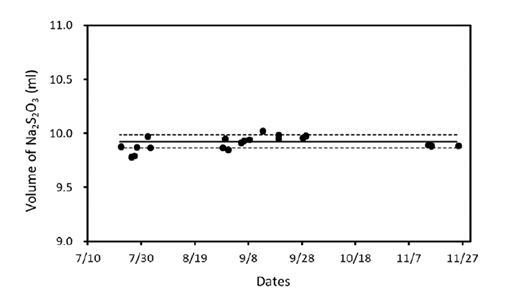
\includegraphics{E:/R/SOP/SOP_C06_COD/images/C06_image2_티오황산나트륨 부피.png}
\caption{캡션을 입력하세요}
\end{figure}

\hypertarget{uxbd84uxc11duxc808uxcc28-uxd750uxb984uxb3c4}{%
\section{분석절차 흐름도}\label{uxbd84uxc11duxc808uxcc28-uxd750uxb984uxb3c4}}

\hypertarget{uxcc38uxace0uxc0acuxd56d}{%
\section{참고사항}\label{uxcc38uxace0uxc0acuxd56d}}

화학적산소요구량(COD)를 정량하는 방법에는 산화제의 종류에 따라 중크롬산칼륨(K\textsubscript{2}Cr\textsubscript{2}O\textsubscript{7})법, 과망간산칼륨법이 있고 과망간산칼륨법은 다시 유기물 분해시 pH에 따라 산성 과망간산칼륨법과 알칼리성 과망간산칼륨법으로 나뉜다. 이중 중크롬산칼륨법과 산성 과망간산칼륨법은 산성하에서 염소이온과 산화제가 많이 반응하여 화학적산소요구량(COD) 값이 실제보다 높게 나타나고, 산화된 염소는 유독가스로 발생되기 때문에 해수처럼 염소이온이 많이 함유된 시료에는 산화력은 조금 떨어지지만 알칼리성 과망간산칼륨법이 많이 이용된다.

\hypertarget{adcpuxb97c-uxc774uxc6a9uxd55c-uxd574uxb958uxad00uxce21-uxd45cuxc900uxc6b4uxc601uxc808uxcc28uxc11c}{%
\chapter{ADCP를 이용한 해류관측 표준운영절차서}\label{adcpuxb97c-uxc774uxc6a9uxd55c-uxd574uxb958uxad00uxce21-uxd45cuxc900uxc6b4uxc601uxc808uxcc28uxc11c}}

\hypertarget{uxbaa9uxc801-uxbc0f-uxbc94uxc704-3}{%
\section{목적 및 범위}\label{uxbaa9uxc801-uxbc0f-uxbc94uxc704-3}}

이 표준운영절차서는 Acoustic Doppler Current Profilers(ADCP)를 해저나 수중에 계류(fixed-mounted)하거나 선박에 장착(vessel-mounted)할 때 ADCP의 운영, 유지관리 및 보수, 교정 등을 위한 표준운영절차서이다. 이 표준운영절차서는 ADCP를 연안 및 내륙의 해수나 담수에서 사용할 때 적용가능하다.

\begin{figure}
\centering
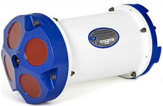
\includegraphics{E:/R/SOP/SOP_P05_ADCP/images/P05_image1_Workhorse Sentinel 300 kHz ADCP.png}
\caption{Workhorse Sentinel 300 kHz ADCP}
\end{figure}

\hypertarget{uxae30uxbcf8-uxb3d9uxc791uxc6d0uxb9ac-1}{%
\section{기본 동작원리}\label{uxae30uxbcf8-uxb3d9uxc791uxc6d0uxb9ac-1}}

ADCP 기본적으로 특정 주파수의 음파를 일정 시간 간격으로 수중으로 방사한다. 이 음파는 물속에 있는 부유물질에 의하여 반사가 되고 이 반사된 음파는 ADCP에 수신이 된다. 부유물질은 해류와 함께 이동하므로, ADCP에서 보낸 음파와 부유물질에 반사되어 ADCP로 되돌아온 음파 간에는 도플러효과에 의해 주파수 차이가 발생한다. ADCP는 되돌아오는 음파의 시간과 주파수 차이를 이용하여 해류의 수심별 속도와 방향을 측정한다. 선박에 장착하는 ADCP는 파장이 긴 음파를 발생시켜서 해저면을 관측 하는 데에도 사용된다. 이 선박장착 ADCP는 배가 항해하면서 수심을 측정하는데도 사용되며 해저에 대한 ADCP의 상대 속도와 방향을 측정할 수 있다.

\hypertarget{uxc6b4uxc601uxbc29uxbc95}{%
\section{운영방법}\label{uxc6b4uxc601uxbc29uxbc95}}

계류형 ADCP의 경우 데이터는 내부의 메인보드 및 메모리에서 계산되고 저장되며 선박장착형 ADCP는 케이블을 통해 데이터를 PC에 전송하여 PC에서 데이터를 계산하고 저장한다. 데이터는 파일로 저장이 되며 사용자가 데이터를 가공할 수 있도록 소프트웨어에서 여러 가지 자료처리 도구를 제공한다. 계류형 ADCP와 선박장착형 ADCP에서의 자료처리 프로그램이 다소 다르기 때문에 각각에 맞게 처리되어야 한다.

\hypertarget{uxc7a5uxbe44uxc758-uxc2a4uxd399}{%
\section{장비의 스펙}\label{uxc7a5uxbe44uxc758-uxc2a4uxd399}}

ADCP는 대부분의 해양환경에서 유속을 측정할 수 있지만, 사용되는 주파수에 따라서 사용 가능 거리와 최대 측정 가능 거리가 다르다. 주파수에 따른 ADCP의 최대 측정 가능 거리는 아래 표와 같다(표 2.1).

예를 들면 300 kHz ADCP의 경우 약 150m 정도까지 측정가능하며, 이 제한 거리를 넘어서면 되돌아오는 음파의 에너지가 너무 작아서 수신을 할 수 없다. ADCP가 방사하는 음파의 주파수가 낮을수록 음파의 전송거리가 더 길어지지만, 해상도는 그만큼 낮아지게 된다. 또한, 계류형 ADCP의 경우 위로 음파를 전송할 때 해수면 근처에서는 사이드 로브 간섭(side lobe interference)으로 인해 자료의 질이 떨어진다. 반대로 선박장착형 ADCP는 해저 부근의 자료 질이 떨어진다.

\hypertarget{uxc801uxc6a9}{%
\section{적용}\label{uxc801uxc6a9}}

3.1. 해양 관측을 위해 한국해양연구원의 ADCP를 사용할 경우, ADCP의 운영, 유지관리, 보수 및 교정을 위해서 반드시 이 표준운영절차서를 따라야 한다.\\
3.2. 관측을 하기 전에 Teledyne RD Instrument's PlanADCP software로 배터리 수명과 데이터 저장 용량이 적절한지 파악한다.\\
3.3. 기존의 배터리에 새로운 배터리를 추가할 경우 내부의 마그네틱 플럭스게이트 컴퍼스에 의한 자기장의 미세변화를 제거하기 위한 교정 작업이 필요하다.\\
3.4. ADCP는 내부에 모터와 같은 부분이 없어서 전자파 장애 현상이 발생되지는 않지만, 내부의 센서들이 전자파에 상당히 민감하다는 것을 유념해야 한다. 이뿐만 아니라 출장 전 장비를 계류하고자 하는 곳의 수심을 잘 파악하여 수심 제한에 맞는 스펙의 장비를 선정하고 패키지 한다.

\hypertarget{uxc7a5uxbe44uxad6cuxc131-1}{%
\section{장비구성}\label{uxc7a5uxbe44uxad6cuxc131-1}}

4.1. 계류형 ADCP의 경우, 모든 모델명의 ADCP는 정해진 지점에서 일정 시간 간격으로 해수면 아래 수층에 대한 유속을 측정한다. 일반적으로 센서는 송·수신 역할을 하는 4개의 트랜스듀서, 온도 셀, 방향(tilt) 센서, 플럭스게이트(fluxgate) 컴퍼스 그리고 압력센서(옵션사항)로 구성되어 있다. 이 모든 구성요소들은 일반적으로 PVC 하우징 안에 내장되며, ADCP는 음향분리기(acoustic releaser, Benthos Model 875-A or 865-A), 신호발생기(Pinger, RJE Model ULB-364/37), 그리고 연결 줄과 함께 다중 ADCP 회수체계(그림 4.1)를 구성한다. 그림 4.1 (d)는 대략 수심이 40 m(즉, 조류가 적은)정도 되는 곳에 ADCP를 계류한 모식도이다. 신호발생기는 스쿠버 다이버가 다중 ADCP 회수체계를 잘 찾을 수 있도록 해주며, 배위로 인양할 경우 연결 줄을 갈고리에 걸어서 올리면 된다. 보통 ADCP의 회수는 해수면에서 송수파기(送受波機, transducer)로 음향분리기를 향해 음파를 발생시켜 음향분리기의 위치를 찾게 된다. 특별히 30m 이상의 깊은 수심에서는 다중 ADCP 회수체계를 구성할 때는 time-out release를 사용하는 것을 추천한다.

4.1.1. 음향 트랜스듀서 헤드(Acoustic Transducer Head)\\
4.1.1.1. 트랜스듀서 3개는 유속(u, v, w)을 측정하고 나머지 1개는 유속 오차 정도를 산정한다. 송수신기 헤드(Acoustic Transducer Head)는 원통 모양의 하우징이다. 송수신 전자장치(transceiver electronic)가 들어있고, 음향송수신부 헤드는 4개의 piezoceramic acoustic transducer로 되어 있다. 4개의 송수신기는 서로 90°씩 떨어져 있고 각 헤드는 25°씩 기울어져 있다. 송수신부 헤드(transduce head)는 폴리우레탄으로 만들어져 있다. 4개의 transducer(송수신부)는 정해진 주파수(300 kHz, 600kHz, 1.2 MHz 등)의 음향펄스(acoustic pulse)를 동시에 전송한다.

4.1.2. 방향 sensor는 움직이는 부분 없이 고정된 모양의 나침반 센서이다. 이 센서는 자기장과 tilt(pitch와 roll)를 측정한다. Compass 방향(heading)은 이러한 측정에 기초해 계산된다. Heading direction은 북쪽과 센서 사이의 각도이다. Micro- controller는 3가지 축으로 지구의 자기장을 측정한다. 이 3가지 축 x, y, z는 서로 직각이다. Tilt-x와 tilt-y도 측정할 수 있다. 또한 tilt를 알면, heading은 세 축의 magnetic field와 tilt로부터 수학적으로 계산된다. 결과는 RS232나 CAN bus에 나타난다. 여기서 결과라 함은 heading과 pitch, roll을 말한다.

\begin{figure}
\centering
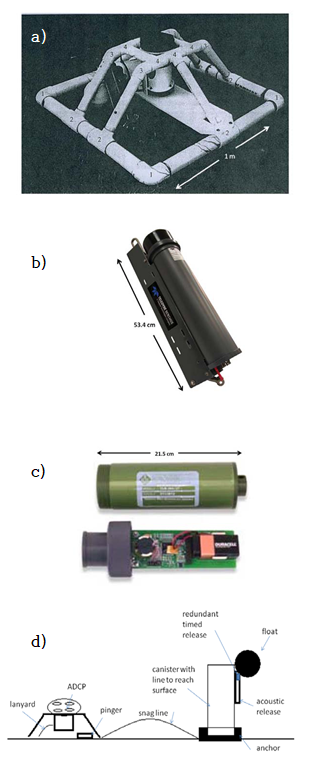
\includegraphics{E:/R/SOP/SOP_P05_ADCP/images/P05_image2_ADCP recovery system.png}
\caption{ADCP recovery system: a) mount, b) acoustic release, c) pinger, and d) detailed configuration for on-fixed deployment}
\end{figure}

4.1.1. 온도센서
4.1.2. 압력센서

4.2. Vessel-mounted ADCP의 경우, ADCP는 움직이는 플랫폼(ex. 보트 혹은 배)에 부착된다. 마찬가지로 4개의 도플러 트랜스듀서, 온도 셀, 틸트 센서, 플럭스게이트 컴퍼스로 구성되어있으며 ADCP가 그림 3처럼 아래 방향을 트래킹 할 수 있도록 구성이 된다. ADCP는 수직 막대기에 두 개의 호스 클램프와 케이블 그리고 바다에 빠지지 않도록 묶여있다. 그리고 ADCP와 노트북 컴퓨터를 케이블로 연결하여 데이터를 받을 수 있으며, 또한 DGPS로부터 GGA-mode(혹은 GSA-mode) 데이터를 전송받을 수 있다.

\begin{figure}
\centering
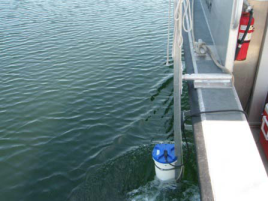
\includegraphics{E:/R/SOP/SOP_P05_ADCP/images/P05_image3_vessel mounted ADCP의 모습.png}
\caption{vessel-mounted ADCP의 모습}
\end{figure}

\hypertarget{uxc7a5uxbe44uxc6b4uxc601uxc790uxc758-uxc790uxaca9uxc694uxac74-uxbc0f-uxcc45uxc784uxc0acuxd56d}{%
\section{장비운영자의 자격요건 및 책임사항}\label{uxc7a5uxbe44uxc6b4uxc601uxc790uxc758-uxc790uxaca9uxc694uxac74-uxbc0f-uxcc45uxc784uxc0acuxd56d}}

5.1. ADCP를 현장에서 안정적으로 운영하기 위해서는 일반적으로 배 운영자(선장)에 더불어 2명의 장비운영 전문가가 필요하다.

5.2. 장비운영 전문가를 ADCP 장비와 관련 소프트웨어 사용에 익숙하도록 훈련을 해야 한다. 뿐만 아니라 장비운영 전문가는 워터 샘플링에도 경험을 갖고 있어야 한다. 장비운영 전문가는 ADCP를 많이 사용한 경험이 반드시 있어야 한다.

5.3. 표류 구조물(ex.부이) 그리고 배 위에서 일을 할 때 안전 절차에 대한 훈련이 되어있어야 한다. 뿐만 아니라 위험한 화학물질(ADCP 트랜스듀서 헤드 위에 칠해진 anti-foul paint)을 다루어본 경험이 반드시 있어야 한다.

\hypertarget{uxbd80uxc18duxd488-uxbc0f-uxc18cuxbaa8uxd488}{%
\section{부속품 및 소모품}\label{uxbd80uxc18duxd488-uxbc0f-uxc18cuxbaa8uxd488}}

1.1. 구명조끼와 우비 준비

1.2. 합성고무 장갑, 가죽장갑, 네오프렌 장갑을 준비

1.3. fixed-mounted 계류의 경우(부록 B참고):

\begin{verbatim}
1.3.1. ADCP battery 팩 교환 (그림6.1 참조)
1.3.2. 교정장비(노트북, 케이블, 교정요원, 틸트 블록)
1.3.3. 데이터를 다운 받을 노트북, mounts, shackles, tackle 그리고 recovery system
1.3.4. 필드 로그(부록 A참조)
1.3.5. 체크리스트와 ADCP 패키징 박스 (부록 B참조)
1.3.6. recovery line 과 tackle
\end{verbatim}

1.4. vessel-mounted의 경우(부록 B 참고):

\begin{verbatim}
1.4.1. ADCP 소프트웨어가 설치된 노트북
1.4.2. 배로부터 DGPS와의 인터페이스(필요할 경우)
1.4.3. ADCP 통신 케이블, 파워 케이블
1.4.4. 필드 로그(부록 B참조)
1.4.5. 체크리스트와 ADCP 패키징 박스 (부록 D, E참조)
\end{verbatim}

\begin{figure}
\centering
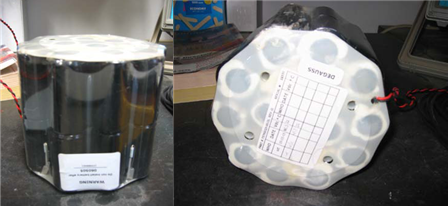
\includegraphics{E:/R/SOP/SOP_P05_ADCP/images/P05_image4_fixed mounted 계류를 위한 배터리팩 교환.png}
\caption{fixed-mounted 계류를 위한 배터리팩 교환}
\end{figure}

\hypertarget{uxc6b4uxc601uxc808uxcc28-1}{%
\section{운영절차}\label{uxc6b4uxc601uxc808uxcc28-1}}

\hypertarget{uxcd9cuxc7a5-uxbc0f-uxacc4uxb958uxc900uxbe44}{%
\subsection{출장 및 계류준비}\label{uxcd9cuxc7a5-uxbc0f-uxacc4uxb958uxc900uxbe44}}

1.1.1. 배에 승선하기 전에 필드 워크 플랜을 위한 계획을 준비한다.(부록 A 참조)\\
1.1.2. ADCP의 계류 방법(fixed 혹은 vessel)에 따라 부록 B를 참고하여 출장차량에 짐을 싣는다.

\hypertarget{uxd574uxc800uxc5d0-adcpuxb97c-uxacc4uxb958uxd560-uxacbduxc6b0}{%
\subsection{해저에 ADCP를 계류할 경우}\label{uxd574uxc800uxc5d0-adcpuxb97c-uxacc4uxb958uxd560-uxacbduxc6b0}}

1.2.1. ADCP의 내부의 센서들이 전자기 필드에 상당히 민감하기 때문에, 계류하고자 하는 위치에 해저 케이블이 없는지 확인하여야 한다. 만약 ADCP 근처에 사람이 만든 전자파 필드가 형성되어 있을 경우 e, v, w components를 rotate하기 위해 ADCP 내부의 플럭스게이트 마그네토미터에 의존하기 보다는 beam 좌표계에서 데이터를 수집하는데 더 주의를 기울인다.

1.2.2. 계류를 어떻게 할 것인가를 계획한다. 일반적으로 6분의 시간간격으로 데이터를 수집하도록 셋팅을 한다. 90개의 데이터를 평균하며, ADCP가 배터리 수명을 연장하기 위해서 4.5분 동안 전원이 꺼지도록 설정한다. PlanADCP software를 통해서 duration, vertical resolution(bin size), 배터리 수명 등에 대한 계산을 할 수 있다. 현재 보유하고 있는 ADCP의 계류수심은 최대 100미터 이고, 조류의 세기에 따라 다르다. ADCP안에 32MB의 저장 메모리 카드가 있으며, 필요에 따라 이 메모리 용량을 업그레이드 할 수 있다. ADCP의 트랜스듀서 부분에 자연침식(생물부착, 빛 투과, 시간의 흐름) 가능성에 따라서 트랜스듀서 부분을 보호해야 한다. Marine fixed paint를 사용하여(9.0 참조)보호하고 있는데 이것은 다른 제품에 비해 유독성이 덜 하다. 일반적으로 선박부착형 ADCP의 경우는 배에 설치하여 해류관측을 하는 시간이 짧기 때문에 biofouling에 대한 대비를 할 필요가 없다.

1.2.3. 아래의 순서대로 ADCP를 준비한다.

\begin{verbatim}
1.1.1.1. 새 배터리팩을 준비한다(그림4 참조). 배터리를 교환하기 위해서 ADCP의 아래쪽(헤드에서 먼 뒤쪽)을 연다. 아래쪽을 열 때 ADCP 하우징 안에 있는 beam 3개가 보이고 헤드의 위치를 확인하면서 연다. 그리고 닫을 때도 마찬가지로 한다. RDI에서 ADCP의 하우징의 실링에 문제가 있다는 것을 발견하였기 때문에 최근에는 ADCP 표면을 실링을 한다. 배터리팩의 끝부분에 있는 볼트를 조심하여 제거한다(구형 배터리와 건조제(방습제)를 제거한다). 고무밴드의 위치를 주의깊게 살펴서 회로 기판으로부터 건조제가 닫지 않도록 한다. 사실 배터리팩을 트랜스듀서의 헤드부분을 열어서 교체할 수도 있지만, 경험상으로 그렇게 하지 않기를 권한다. 필자의 생각에는 커넥터의 끝부분을 통해서 배터리를 교환하는 것이 더 쉽다고 생각한다. ADCP의 안쪽 그리고 바깥쪽은 동일하게 실링이 되어있으나, 매번 끝부분의 cap이 열리게 됨에 따라 ADCP의 내부에 마이너스압력이 생성될 가능성이 있어서 진공효과를 발생시키게 된다. 이 진공효과로 인해 ADCP 안으로 습기가 들어올 수 있다. 만약에 O-ring 부분에 이물질이 존재할 경우, 그 사이로 침수가 일어날 수 있으며 ADCP의 전자회로에 치명적인 영향을 줄 수 있다. 이 문제가 발생하였을 경우 주저 없이 다음 사람에게 연락을 하면 도움이 받을 수 있다. Matt Burdyny, Field Service Engineer, Teledyne-RD Instruments: Acoustic Doppler Solutions
1.1.1.2. ADCP안에 있는 구 건조제를 꼭 새 건조제로 교제한다.
1.1.1.3. ADCP의 뒷부분을 열다가 ADCP beam 3를 건드리면 중요한 문제를 일으킬 수 있다. 배터리 팩을 ADCP에 교체한 후 길게 늘어진 전선을 고무밴드로 배터리 팩의 옆 부분에 감는다.
1.1.1.4. 뒷받침판과 워셔 그리고 윙너트를 추가한다. 윙너트 부분에 고무밴드를 감아 건조제를 매달아서 ADCP의 회로기판에 닫지 않도록 한다.
1.1.1.5. O-ring에 Dow Corning 111 valve lubricant 제품과 실링용 실리콘 그리스를 다시 바른다. O-ring 부분에 모래나 먼지와 같은 이물질이 존재 하지 않도록 확실하게 제거한다.
1.1.1.6. 바깥쪽 볼트를 채우고 안쪽으로 너트를 채운다. 각각의 한 개의 볼트의 헤드와 2개의 너트 아래에 워셔를 끼운다.
1.1.1.2. PlanADCP 소프트웨어를 통해 계류 방법을 계획한다. (www.rdinstruments.com for latest details). 
1.1.1.3. 마그네틱 필드가 존재하지 않는 환경에서 새 배터리를 교환한 ADCP를 교정한다. 이를 위해서 소프트웨어가 깔려있는 노트북, 케이블, 그리고 교정요원이 필요하다. ADCP의 시간을 GMT로 맞춘다.
\end{verbatim}

\begin{enumerate}
\def\labelenumi{(\arabic{enumi})}
\item
  교정요원\\
  가. ADCP의 헤드를 1-2-3-4 순차적으로 브러쉬한다.\\
  나. Rotate flat, 360 degrees on primary axis.\\
  다. Rotate pitch/roll. lift by 10.20 degrees up on side 3 with a non-magnetic tilting block, rotate 360 degrees on primary axis.\\
  라. Rotate roll/pitch. lift by 10-20 degrees up on adjacent side, 360 degrees on primary axis.\\
  마. Final rotation. not as critical. Rotate somewhere between (and not as much), 360 degrees on primary axis.

  1.1.1.1. 구 데이터를 ErAsE를 통해 지운다.\\
  1.1.1.2. 교정작업을 완료 한 후, 대기 중 혹은 선상에서 물기가 없는 지역에서 데이터 수집을 시작한다.\\
  1.1.1.3. Workhorse Sentinel ADCP는 컴퓨터와 통신을 할 때 대략 2.2W 파워를 소모하는데 한 개의 배터리 팩으로 대략 5일정도 쓸 수 있다. ADCP가 통신하지 않을 때는 거의 1mW 이하의 파워를 소모한다. 일반적으로 새 배터리 팩으로 교환한 ADCP는 대략 3달 정도 계류할 수 있는데 여러 가지 변수에 따라 바뀔 수 있기 때문에 제조사의 소프트웨어(ADCPlan)를 통해 결정하는 것이 가장 좋은 방법이다.\\
  1.1.1.4. 계류를 위한 여러 가지 도구 및 체인의 최종 구성도는 계류 지역에 따라 그리고 그 장비의 운영자의 경험에 따라 다를 수 있다. 일반적으로 장비 계류 및 설치를 위한 모습이 그림 7.1에 나타나있다.
\end{enumerate}

\begin{figure}
\centering
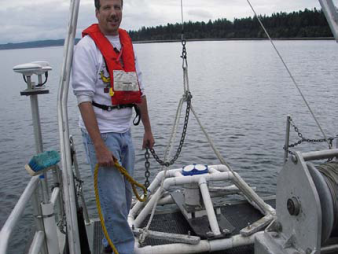
\includegraphics{E:/R/SOP/SOP_P05_ADCP/images/P05_image5_ADCP 계류를 하기 위한 mount의 모습.png}
\caption{DCP 계류를 하기위한 mount의 모습}
\end{figure}

1.1.1. 음향분리기(Acoustic Release)를 테스트 하고 준비한다.

\begin{verbatim}
1.1.1.1. 음향분리기는 반드시 사용하기 전에 청소하고 미리 테스트가 되어있어야 한다. 분리를 미리 테스트하기 위해서는 새로운 배터리로 교환하고 공기 중에서 분리를 트리거 하여  성능을 검사한다. 이것은 반드시 출장 전에 시행 되어야 한다. 
\end{verbatim}

1.1.2. 회수 절차

\begin{verbatim}
 1.1.2.1. 장비의 회수
 ADCP 장비를 회수하기 위한 방법은 음향분리기 트랜스듀서를 수중에 넣어 음향분리기를 찾는 것이다. 이때 트랜스듀서는 Benthos deck box(그림 7-2참조)와 연결되어있는데, 이 deck box는 배의 110V AC power에 연결되어있다. 트랜스듀서는 deck box와 연결되어있는데 트랜스듀서를 사용하기 위해서는 기술이 있는 운영자가 필요하다. 음파는 수중에서 밀도차이로 인해 쉽게 산란된다. 최악의 경우, 음향분리기와 통신이 안 되는 경우도 발생할 수 있다. 각각의 분리기는 특정주파수(ex. 10 kHz)로 고정되어있고 분리기의 코드(ex. 'A')가 운영자에 의해서 선정되어야 한다. 배 아래에서 분리기를 찾는 작업을 몇 번 계속 시도를 하고 관찰을 한다. 분리기를 찾는데 성공하였으면, 배의 갈고리를 이용하여 ADCP를 회수한다. 회수할 때 그림 7.3과 같은 파워윈치를 사용한다.   
\end{verbatim}

\begin{figure}
\centering
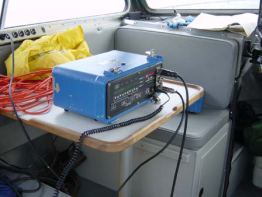
\includegraphics{E:/R/SOP/SOP_P05_ADCP/images/P05_image6_hydrophone이 연결된 Benthos type deck box.png}
\caption{hydrophone이 연결된 Benthos-type deck box}
\end{figure}

\begin{figure}
\centering
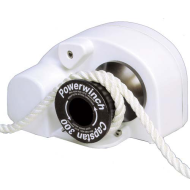
\includegraphics{E:/R/SOP/SOP_P05_ADCP/images/P05_image7_ADCP mount를 회수하기 위한 파워윈치.png}
\caption{ADCP mount를 회수하기 위한 파워윈치}
\end{figure}

만약에 음향분리기가 작동을 하지 않을 경우, ADCP를 찾을 수 없기 때문에 상황이 된다면 갈고리를 이용해야 한다. 처음에 계류를 했던 위치를 적어놓은 야장에서 연결 줄의 위치를 파악한다. ADCP 계류체계를 찾기 위해서는 선장의 역할이 중요하다. 만약에 ADCP 계류체계를 찾는데 실패했을 경우, 음향분리기의 배터리 수명이 다할 수 있기 때문에 ADCP를 재 회수하기 위한 작업이 빠른 시간 내에 이루어져야 한다. 필요에 따라서는 갈고리 후크 그리고 스쿠버 다이버 혹은 ROV의 도움으로 장비를 회수하는데 도움을 받아야 한다.

1.1.1.1. 데이터 복원
ADCP에 데이터 케이블을 연결하여 WinSC 소프트웨어를 통해서 데이터를 다운 받거나 ADCP의 트랜스듀서쪽 헤드를 열어서 직접 PCMIA데이터 카드를 꺼내서 노트북에 연결하여 데이터를 다운받을 수 있다. 보통 데이터 케이블을 통한 시리얼 전송의 경우 한 시간 혹은 그 이상이 걸리지만 ADCP의 케이스를 열지 않고 데이터를 다운 받을 수 있는 장점이 있다.

1.1.1. 보관 절차\\
1.1.1.1. 모든 기·장비는 깨끗한 물로 씻어야 하며, 부착된 이물질을 제거해야한다. 그리고 보관하기 전에 잘 건조시켜야 한다. 미생물부착으로 인한 biofouling이 제거되어야 하는데, 특히 ADCP의 트랜스듀서 헤드부분을 청소 할 때는 상당한 주의를 기울여야 한다.\\
1.1.1.2. 모든 기어는 보관장소에 제대로 보관이 되어야 한다. 보관에 대한 의문점이 있으면 출장 코디네이터에게 문의를 한다. 밧줄은 로프 보관 장소에 저장하며 mount는 야외에 보관하는 것도 괜찮으나 직사광선에 바로 노출된 장소는 피하는 것이 좋다. ADCP와 음향분리기 그리고 신호발생기 등은 해양관측장비 보관 장소에 잘 포장하여 보관한다.

\hypertarget{uxad00uxb9ac-1}{%
\section{관리}\label{uxad00uxb9ac-1}}

\hypertarget{uxb370uxc774uxd130-uxad00uxb9ac-1}{%
\subsection{데이터 관리}\label{uxb370uxc774uxd130-uxad00uxb9ac-1}}

\hypertarget{uxae30uxb85duxbb3c-uxad00uxb9ac-1}{%
\subsection{기록물 관리}\label{uxae30uxb85duxbb3c-uxad00uxb9ac-1}}

1.2.1. 수중계류 ADCP가 설치된 각각의 사이트에 대한 표준화된 필드 로그 시트(부록 A참조)를 사용하여서 필드의 상태, 위치, 장비의 시리얼 넘버 그리고 중요하게 고려되어야 할 다른 정보들 등과 같은 사이트에 대한 정보를 반드시 기록한다. 선박장착 ADCP의 경우, 마찬가지로 부록 B를 참고하여 필드 로그시트를 사용하여 기록을 한다. Operation Center(OC)에 돌아왔을 때, 장비는 반드시 세척되어야 하고 장기간의 보관을 위해서 건조되어야 한다. 수중계류와 선박장착의 경우 모두 출장이 완료된 후 필드 스태프에 의해서 그 로그시트는 전자 데이터베이스에 입력되어야 한다.

1.2.2. 수중계류 ADCP의 저장디렉토리는 다음과 같다.
( 웹하드 디렉토리 )

1.2.3. 선박장착 ADCP의 저장디렉토리는 다음과 같다.
( 웹하드 디렉토리 )

\hypertarget{uxc7a5uxbe44-uxad00uxb9ac-1}{%
\subsection{장비 관리}\label{uxc7a5uxbe44-uxad00uxb9ac-1}}

1.3.1. 주기적 점검 사항
1.3.1.1. 수중계류 ADCP의 보수점검은 계류 시에 매번 시행한다. ADCP 통제 및 자료저자용 컴퓨터의 유지보수 간격은 1개월을 원칙으로 한다.

1.3.2. ADCP 보수점검 사항은 아래와 같다.
(1) 입출력 케이블과 더미 플러그
(2) 유속계 분해
(3) 유속계 조립
(4) 배터리 팩
(5) 나침반의 방위 보정
(6) 퓨즈 교체
(7) 통신 설정
(8) 방습제
(9) 계류를 위한 유속계 밀봉
(10) 부착생물 방지
(11) 온도센서 관리
(12) 압력센서 관리

1.1.1. 입출력 케이블과 더미 플러그

\begin{verbatim}
1.1.1.1. 수중 케이블, 입출력 케이블, 더미 플러그는 수중에서 방수와 절연이 되어야 한다.
1.1.1.2. 입출력 케이블이나 더미 플러그를 장비로부터 빼 내고자 할 때는 먼저 유지고무줄(retaining strap)을 위로 올리고, 케이블을 장치 단자에 가깝게 잡고, 단자의 방향과 수평으로 잡아당겨 분리한다.
1.1.1.3. 입출력 단자 또는 더미 플러그를 장비에 연결하고자 할 때는 연결단자와 평행하게 밀어야 한다. DC-111 윤활제를 장비 연결단자의 고무 부분에 가볍게 바르면 연결에 도움이 된다. 유지고무줄을 굴려서 단자에 맞춘다.
\end{verbatim}

\begin{figure}
\centering
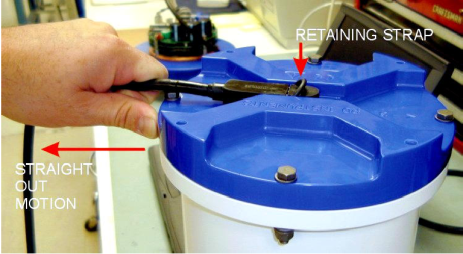
\includegraphics{E:/R/SOP/SOP_P05_ADCP/images/P05_image8_입출력 단자 제거 모습.png}
\caption{입출력 단자 제거 모습}
\end{figure}

1.1.1. 유속계 분해
1.1.1.1. 밑 뚜껑 제거
(1) 장비를 건조시킨다. 트랜스듀서 면에 부드러운 받침을 댄다. 장치에 공급되는 전원을 제거한다. 입출력 케이블과 더미 케이블을 제거한다.
(2) 4개의 볼트를 느슨하게 풀어 준다. 모든 볼트를 느슨하게 푼 후 볼트를 밑 뚜껑에서 분리한다. 조심스럽게 장비의 틀에서 밑 뚜껑을 공통 모드 초크에 연결된 잭에 접근할 수 있을 때까지 들어 올린다.
(3) 내부 입출력 케이블 연결자의 양 측면을 눌러 공통 모드 초크로부터 분리시킨다.
(4) O 링과 접촉되는 면을 먼지가 나지 않는 천으로 부드럽게 닦아 준다. 접촉면이 손상되지 않았는지 검사한다. O 링에 작은 흠집이라도 있으면 물이 센다.
1.1.1.2. 트랜스듀서 상부 조립부품 제거
(1) 장비에 연결된 모든 전원을 제거한다.
(2) 입출력 케이블과 더미 플러그를 입출력 단자로부터 제거한다.
(3) 장비를 밑 뚜껑을 아래로 하고 세운다.
(4) 모든 볼트를 느슨하게 풀어준다. 모든 볼트가 느슨해지면 볼트를 상부 조립부품에서 분리한다.
(5) 조심스럽게 들어 올려 공통 모드 초크에 연결된 단자에 접근할 수 있을 때까지 들어 올린다.
(6) 내부 입출력 케이블 연결자의 양 측면을 눌러 공통 모드 초크로부터 분리시킨다.
(7) O 링과 접촉되는 면을 먼지가 나지 않는 천으로 부드럽게 닦아 준다. 접촉면이 손상되지 않았는지 검사한다.

1.1.2. 유속계 조립
1.1.2.1. 장비를 계류하기 위하여 밀봉한다면 ADCP 밀봉 방법에 따라 모든 항목을 수행하여야 한다.
1.1.2.2. 모든 인쇄된 회로보드, 케이블, 나사가 장착되어야 한다.
1.1.2.3. ADCP 밀봉 전에 두 개의 새로운 방습제 백을 넣어야 한다.
1.1.1.1. O 링 검사와 교체
(1) 계류의 성공여부는 O 링의 상태에 달려있다. 계류에 사용된 O 링은 교체하는 것이 바람직하다. O 링의 유지보수 작업은 최종적으로 한다.
(2) O 링 검사: 맨 눈으로 보아 O 링은 갈라지거나 찌그러지거나 이물질이 들어가거나 물결무늬가 있어서는 안 된다. O 링은 매끈하고 일정한 형태를 띠어야 한다. 결점은 0.1 mm보다 작아야 한다.
(3) O 링을 닦고 결점을 검사한다. 이물질의 결점, 부식, 구멍이 없어야 한다. 손톱으로 지나가 보아서 느낌이 없으면 사소한 것이지만 그렇지 않으면 손상되었으므로 교체해야 한다.
(4) O 링 결점이 플라스틱 본체에 있어 불룩하게 된 흠집이라면 샌드페이퍼(60 망)을 사용하여 갈아 낼 수 있다. 이 때 다른 상처가 생기지 않도록 한다.
(5) DC-111 윤활제를 O 링에 얇게 나른다. 고무장갑을 이용한다. 작업을 하면서 누수의 원인이 되는 실이나 실보무라지가 묻지 않도록 한다.
1.1.1.1. 밑 뚜껑 교체
(1) 부드러운 물건으로 트랜스듀서 밑에 바치고 세운다.
(2) 본체의 O 링을 검사하고, 닦고, 윤활제를 바른다. O 링에 실리콘 윤활제를 가볍게 바른다. 지나치게 많은 윤활제를 바르면 윤활제를 바르지 않는 것 보다 더욱 해로울 수 있다.
(3) 내부 입출력 단자를 공통 모드 초크에 연결한다.
(4) 밑 뚜껑을 본체에 넣어 나사구멍에 맞춘다. 3번 빔과 밑 뚜껑에 표시된 방향이 일치되어야 한다.
(5) 볼트 너트를 넣어서 조여 준다.
1.1.1.2. 트랜스듀서 상부 조립 부품 교체
(1) 밑 뚜껑 교체와 같은 방식으로 진행한다.

1.1.2. 배터리 팩
1.1.2.1. 배터리 전압이 30 VDC 이하이면 교체하여야 한다.

1.1.3. 컴퍼스 보정
1.1.3.1. 배터리 교체 후에는 컴퍼스를 보정해야 한다.

1.1.4. 퓨즈 교체
1.1.4.1. POI 보드의 퓨즈를 점검하여 교체한다.

1.1.5. 통신 설정
1.1.5.1. 유속계와 컴퓨터가 같은 통신 방식을 하여야 한다. 유속계는 RS-232와 RS-422를 변경할 수 있는 스위치가 있다. 컴퓨터 통신 체계에 맞는 방식을 선택하여야 한다.

1.1.6. 방습제
1.1.6.1. 방습제는 플라스틱 본체 장비를 계류할 때 필수적이다. 방습제는 일반적인 방의 습기를 빠르게 흡수한다. 새로운 방습제의 평균 무게는 7.2 그램이다. 사용된 방습제는 무게가 8.4 그램에서 9 그램이다. 사용된 방습제는 250°에서 14시간동안이면 건조시킬 수 있다. 계류하기 전 또는 보관하기 전에 방습제를 교체해야 한다.

1.1.7. 계류를 위한 유속계 밀봉
1.1.7.1. 나사, PC 카드, 배터리 팩, 방습제를 확인하고 밑 뚜껑을 조립한다.

1.1.8. 부착생물 방지
1.1.8.1. 100 m 이내의 얕은 수심의 따뜻한 해수에서 계류할 때는 부착생물이 많이 붙는다. 매주 트랜스듀서를 닦아 줄 수 없다면 부착생물 방지용 그리스를 발라준다.

1.1.9. 온도센서 관리
1.1.9.1. 온도센서에는 생물부착방지 페인트를 바르지 않는다. 부착생물을 가능한 빨리 닦아준다.

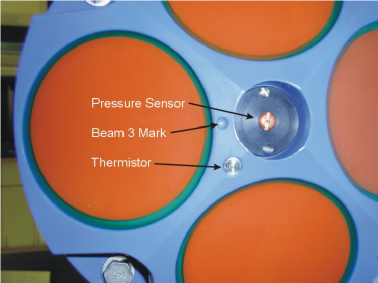
\includegraphics{E:/R/SOP/SOP_P05_ADCP/images/P05_image9_온도센서와 압력센서의 모습.png}
1.1.1. 압력센서 관리
1.1.1.1. 압력을 측정하기 위해서는 구리나사의 구멍에 물이 흘러 들어가야 하는데 그 구멍이 쉽게 막힌다. 그 구리나사를 분해하여 잘 닦아 준다.

\begin{figure}
\centering
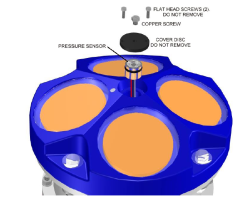
\includegraphics{E:/R/SOP/SOP_P05_ADCP/images/P05_image10_초음파 유속계의 압력센서.png}
\caption{초음파 유속계의 압력센서}
\end{figure}

1.1.1. ADCP 시험
1.1.1.1. ADCP를 그림8.4와 같이 연결한다. 유속계를 버킷 물속에 넣어 둔다. ADCP가 물속에 있지 않으면 몇 가지 시험이 실패한다.
1.1.1.2. BBTalk 프로그램을 실행한다.
1.1.1.3. ADCP 시험 마법사가 시행되도록 키를 누른다. 시험 결과가 스크린에 나타나고 WH\_RSLTS.txt에 저장된다. WH\_RSLTS.tx 파일은 BBTalk가 실행되는 디렉토리와 같은 장소에 정장되지 않는다.

\begin{figure}
\centering
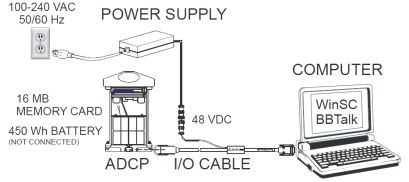
\includegraphics{E:/R/SOP/SOP_P05_ADCP/images/P05_image11_ADCP 시험을 위한 연결도.png}
\caption{ADCP 시험을 위한 연결도}
\end{figure}

1.1.1.1. 관측 전 점검 사항(부록 B 참조)

1.1.1.2. 관측 후 점검 사항(부록 B 참조)

\hypertarget{uxd488uxc9c8-uxad00uxb9acuxc640-uxd488uxc9c8-uxbcf4uxc99d-1}{%
\section{품질 관리와 품질 보증}\label{uxd488uxc9c8-uxad00uxb9acuxc640-uxd488uxc9c8-uxbcf4uxc99d-1}}

\hypertarget{uxd544uxb4dc-uxd488uxc9c8-uxad00uxb9ac}{%
\subsection{필드 품질 관리}\label{uxd544uxb4dc-uxd488uxc9c8-uxad00uxb9ac}}

1.1.1. ADCP의 달려 있는 4번째 트랜스듀서는 유속의 3차원속도(u, v, w)를 측정하는데 있어서 오차 정도를 제공해준다. 트랜스듀서의 헤드부분은 기하학적으로 고정(수평면에서 20도 틀어져 있다)이 되어있기 때문에, 부 정확도를 산정하는 용승/하강을 나타내는 w가 수평 컴포넌트( u(동-서), v(남-북) )보다 커지게 된다. 연구과제의 기획에 따라 달라지겠지만, vessel-mounted ADCP의 품질관리의 경우 여러 번의 품질필터를 거치는 것을 추천한다. 여러 자료의 세트를 한 번의 품질필터를 거치는 것 보다, 한 개의 세트마다 여러 번의 품질필터를 거치는 것이 더 좋다.

\hypertarget{uxb370uxc774uxd130-uxc5d4uxd2b8uxb9acuxc640-uxb85cuxadf8-uxc2dcuxd2b8-uxd488uxc9c8-uxad00uxb9ac}{%
\subsection{데이터 엔트리와 로그 시트 품질 관리}\label{uxb370uxc774uxd130-uxc5d4uxd2b8uxb9acuxc640-uxb85cuxadf8-uxc2dcuxd2b8-uxd488uxc9c8-uxad00uxb9ac}}

1.2.1. 필드 스태프 중 한 사람으로부터 데이터베이스에 입력된 각각의 로그 시트는 다른 스태프가 또 다른 로그 시트를 데이터베이스에 입력할 때 다른 스태프에 의해서 그 전 로그시트가 재검토 되어야 한다. 검토시에 참고가 될 수 있도록 그 로그시트의 작성날짜와 작성한 기술자의 이름을 적어놓는다. 작성된 로그시트들은 최종적으로 ADCP 코디네이터의 책상위에 놓아져야 한다.

\hypertarget{uxc548uxc804uxc0acuxd56d}{%
\section{안전사항}\label{uxc548uxc804uxc0acuxd56d}}

1.1. 모든 필드 스태프들은 Environmental Assessment Program(EAP) Safety Manual의 사항을 완벽히 숙지하고 따라야 하며 특히 부가적으로 추락 방지, 물위에서의 작업, 화학약품 안전사항 그리고 EAP safety manual의 챕터3 부분을 숙지하고 있어야 한다. 보호장비( 합성고무 장갑, 가죽장갑, 등)의 적절한 사용은 필드 스태프의 의무이다.

1.2. MSDS 화학약품에 대한 정보, 저장, 폐기, 그리고 안전사항들을 의무적으로 숙지하고 있어야 한다(MSDS Trilux White = \url{http://www.yachtpaint.com/msds_pdf/YBA068_GBR_ENG.pdf}). EAP HQ safey Manual을 참조한다.

\hypertarget{uxcc38uxace0uxbb38uxd5cc-4}{%
\section{참고문헌}\label{uxcc38uxace0uxbb38uxd5cc-4}}

1.1. Environmental Assessment Program, 2006. Environmental Assessment Program Safety Manual. March 2006. Washington State Department of Ecology. Olympia, WA.

1.2. WorkHorse Sentinel ADCP User's Guide, P/N 957-6163-00 (January 2001), RD Instruments Acoustic Doppler Solutions (Appendix F).

\hypertarget{uxbd80uxb85d-1.-uxd544uxb4dc-uxb85cuxadf8fixed-mounted-adcp}{%
\section{부록 1. 필드 로그(Fixed-mounted ADCP)}\label{uxbd80uxb85d-1.-uxd544uxb4dc-uxb85cuxadf8fixed-mounted-adcp}}

LOG SHEET FOR ADCP BOTTOM DEPLOYMENT

날 짜:\\
배 이름: 선장 이름:\\
출장 장소: 선원 이름:

계류한 ADCP의 위도:\\
계류한 ADCP의 경도:

설치한 앵커 위도: 수심:\\
설치한 앵커 경도:

ADCP로부터 떨어진 태그 라인의 방향 그림(동그라미 안의 X에 표시)

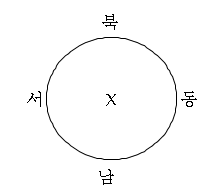
\includegraphics{E:/R/SOP/SOP_P05_ADCP/images/P05_image12_부록1 삽입 사진.png}

날씨:\\
풍속: 풍향:

작업시작

시간: 육지에서 떨어진 거리(m):

Acoustic Release(model 875A)
Serial number:\\
Frequency(Hz):\\
Release code:

Pinger? 예/아니오\\
Snag-line? 예/아니오\\
Timed-release? 예/아니오

\hypertarget{uxbd80uxb85d-2.uxd544uxb4dc-uxb85cuxadf8vessel-mounted-adcp}{%
\section{부록 2.필드 로그(Vessel-mounted ADCP)}\label{uxbd80uxb85d-2.uxd544uxb4dc-uxb85cuxadf8vessel-mounted-adcp}}

LOG SHEET FOR ADCP DATA COLLECTION

날 짜:\\
배 이름: 선장 이름:\\
출장 장소: 선원 이름:

Transect Number:\\
Transect Name:\\
저장파일이름:\\
Configuration 파일 이름:

날씨: 풍속: 풍향:

작업시작

시간: 육지에서 떨어진 거리(m):

Select Bank: Left / Right
Transect Direction (heading):\\
위도:\\
경도:

작업종료

시간: 육지에서 떨어진 거리(m):

Select Bank: Left / Right
Transect Direction (heading):\\
위도:\\
경도:

메모:

\hypertarget{uxbd80uxb85d-3.uxd604uxc7a5-uxc900uxbe44-uxc2dc-uxc900uxbe44uxc0acuxd56d-uxbc0f-uxbb3cuxd488}{%
\section{부록 3.현장 준비 시 준비사항 및 물품}\label{uxbd80uxb85d-3.uxd604uxc7a5-uxc900uxbe44-uxc2dc-uxc900uxbe44uxc0acuxd56d-uxbc0f-uxbb3cuxd488}}

(Bottom-mounted ADCP 체크리스트)
Office \& Electronics

\begin{itemize}
\tightlist
\item
  Laptop Computer (w/ power cord)
\item
  Data stick for backing-up data
\item
  Metal Clipboard
\item
  Float Plan x3 (Section Secretary, Contact, Field)
\item
  Sample Logs
\item
  Tide Table
\item
  Cell Phone (w/ charger)
\item
  Digital Camera
\item
  MSDS
\end{itemize}

OC Field Supplies

\begin{itemize}
\tightlist
\item
  Data cable and power cord for 110-volt ship power (or battery)
\item
  Life Jackets
\item
  Power winch with footswitch
\item
  Buckets
\item
  Mount with ADCP (and new batteries)
\item
  Acoustic release (batteries), deck unit and hydrophone
\item
  Pinger (batteries)
\item
  Chain, tackle, anchor ball for line canister
\item
  Viny float, and line
\item
  Special line that allows release of float from either acoustic or time signal
\item
  Hefty bag to seal line cylinder
\item
  Buoyant (floating) yellow snag-line (50 m, \textgreater{} ½-inch, 5000\# test)
\item
  Hose clamps (or nylon ties), and spares
\item
  Boat hook
\item
  ADCP Rubbermaid Action Packer, Large
\item
  Tool Box (content details listed below)
\item
  Cable to interface with DGPS
\end{itemize}

From Wet Lab

\begin{itemize}
\tightlist
\item
  *Plastic Bags

  \begin{itemize}
  \tightlist
  \item
    *Label, Electrical and Duct Tape\\
  \item
    *Sharpies, Pencils and Pens
  \end{itemize}
\item
  *Connectors
\item
  *Bottle Brushes \& Paper Clip (straightened)
\item
  *Scissors
\item
  *Dummy plugs for ADCP
\item
  *Nitrile Gloves, Med and Large
\item
  *Extra Plastic Beaker
\item
  *Kimwipes
\item
  Deck unit and hydrophone (for recovery)
\end{itemize}

Items packed morning of departure

Contents of Bins\\
Large ADCP Action Packer

\begin{itemize}
\tightlist
\item
  Hose Clamps and/or large nylon ties
\item
  Electrical Tape\\
\item
  Duct Tape\\
\item
  Zip-Ties, various sizes\\
\item
  Spare Parts\\
\item
  Gloves, Nitrile\\
\item
  Sandwich Box with Allen Wrench\\
\item
  Kimwipes\\
\item
  Misc Hardware (screws, nuts, washers, insulators, Teflon tape)\\
\item
  Plastic Beaker\\
\item
  Brushes\\
\item
  Teflon and Wooden Block
\end{itemize}

Toolbox\\
Screwdrivers

\begin{itemize}
\tightlist
\item
  Large flathead\\
\item
  Small flathead\\
\item
  Large Philips\\
\item
  Stubby Philips
\end{itemize}

Pliers

\begin{itemize}
\tightlist
\item
  Large diagonal cutters (for large zip-ties)\\
\item
  Small diagonal cutters (for small zip-ties)\\
\item
  Needle nose\\
\item
  Locking
\end{itemize}

Wrenches

\begin{itemize}
\tightlist
\item
  Adjustable\\
\item
  Ratchet w/ drivers (various)\\
\item
  Combo wrenches (various)\\
\item
  Allen wrenches\\
\item
  Nut drivers (various, 7 mm for heavy duty hose clamps)\\
\item
  Hammer\\
\item
  Electrical tape\\
\item
  Knife\\
\item
  Extra ADCP plugs\\
\item
  Spare nuts, bolts, and ties
\end{itemize}

\hypertarget{uxbd80uxb85d-4.uxd604uxc7a5-uxc900uxbe44-uxc2dc-uxc900uxbe44uxc0acuxd56d-uxbc0f-uxbb3cuxd488}{%
\section{부록 4.현장 준비 시 준비사항 및 물품}\label{uxbd80uxb85d-4.uxd604uxc7a5-uxc900uxbe44-uxc2dc-uxc900uxbe44uxc0acuxd56d-uxbc0f-uxbb3cuxd488}}

(Vessel-mounted ADCP 체크리스트)

Office \& Electronics

\begin{itemize}
\tightlist
\item
  Laptop Computer (w/ power cord)
\item
  Data stick for backing-up data
\item
  Metal Clipboard
\item
  Float Plan x3 Section Secretary, Contact, Field)
\item
  Sample Logs
\item
  Tide Table
\item
  Cell Phone (w/ charger)
\item
  Digital Camera
\item
  MSDS
\end{itemize}

OC Field Supplies

\begin{itemize}
\tightlist
\item
  Data cable and power cord for 110-volt ship power (or battery)
\item
  Life Jackets
\item
  Buckets
\item
  Mount for ADCP to vessel (w/lanyard)
\item
  Boat hook
\item
  ADCP Rubbermaid Action Packer, Large
\item
  Tool Box (content details listed below)
\item
  Cable to interface with DGPS (if desired)
\end{itemize}

From Wet Lab

\begin{itemize}
\tightlist
\item
  *Plastic Bags
\item
  *Label, Electrical and Duct Tape
\item
  *Sharpies, Pencils and Pens
\item
  *Connectors
\item
  *Bottle Brushes \& Paper Clip
  (straightened)
\item
  *Scissors
\item
  *Dummy plugs for ADCP
\item
  *Nitrile Gloves, Med and Large
\item
  *Extra Plastic Beaker
\item
  *Kimwipes
\end{itemize}

Items packed morning of departure\\
Contents of Bins
Large ADCP Action Packer
(some items duplicative of toolbox)

\begin{itemize}
\tightlist
\item
  Hose Clamps and/or large nylon ties
\item
  Electrical Tape
\item
  Duct Tape
\item
  Zip-Ties, various sizes
\item
  Spare Parts
\item
  Gloves, Nitrile
\item
  Sandwich Box with Allen Wrench
\item
  Kimwipes
\item
  Misc Hardware (screws, nuts, washers, insulators, Teflon tape)
\item
  Plastic Beaker
\item
  Brushes
\item
  Teflon and Wooden Blocks
\item
  Sponges
\end{itemize}

Toolbox\\
Screwdrivers

\begin{itemize}
\tightlist
\item
  Large flathead
\item
  Small flathead
\item
  Large Philips
\item
  Stubby Philips
\end{itemize}

Pliers\\
- Large diagonal cutters (for large zip-ties)\\
- Small diagonal cutters (for small zip-ties)\\
- Needle nose\\
- Locking

Wrenches

\begin{itemize}
\tightlist
\item
  Adjustable\\
\item
  Ratchet w/ drivers (various)\\
\item
  Combo wrenches (various)\\
\item
  Allen wrenches\\
\item
  Nut drivers (various, 7 mm for heavy duty hose clamps)\\
\item
  Hammer\\
\item
  Electrical tape\\
\item
  Knife\\
\item
  Extra ADCP plugs\\
\item
  Spare nuts, bolts, and ties
\end{itemize}

\hypertarget{uxcd1duxc9c8uxc18c-uxbd84uxc11d-uxd45cuxc900uxc6b4uxc601uxc808uxcc28uxc11cuxae30uxccb4uxbd84uxc808-uxc790uxb3d9uxc601uxc591uxc5fc-uxbd84uxc11duxae30}{%
\chapter{총질소 분석 표준운영절차서(기체분절 자동영양염 분석기)}\label{uxcd1duxc9c8uxc18c-uxbd84uxc11d-uxd45cuxc900uxc6b4uxc601uxc808uxcc28uxc11cuxae30uxccb4uxbd84uxc808-uxc790uxb3d9uxc601uxc591uxc5fc-uxbd84uxc11duxae30}}

\hypertarget{uxbaa9uxc801-uxbc0f-uxbc94uxc704-4}{%
\section{목적 및 범위}\label{uxbaa9uxc801-uxbc0f-uxbc94uxc704-4}}

총 질소는 유기성 질소와 무기성 질소를 의미한다. 유기성 질소에는 알부미노이드성 질소, 요산이 있고, 무기성 질소는 아질산성, 질산성, 암모니아성 질소가 있다. 오염에 주요 원인이 되는 지표는 무기성 질소이다. 이 분석법은 해수시료의 모든 질소화합물인 무기성 질소, 유기성질소와 입자성질소 등을 자동 전처리 장비를 통해 산화, 분해하여 질산성 질소(NO3-) 형태로 변화시킨 후 카드뮴-구리 환원 칼럼을 이용하여 아질산성 질소(NO2-)로 환원시켜 연속 분절 흐름식(Continuous flow analysis, CFA) 자동 영양염 분석 장비를 이용하여 550nm 파장에서 Sulfanilamide와 NEDD 시약과 반응하여 총 질소를 정량하는 방법이다. 자동 전처리 장비에 주입되는 알칼리성 과황산칼륨 용액은 Method of Seawater Analysis(1999, 3판)에서 제시하는 Mg(OH)2를 발생시키지 않기 위한 NaOH비율을 따르고 있다. 또한 연속 분절 흐름식 자동 영양염 분석 장비는 시료를 공기 방울로 나눔으로 시료의 분산을 막고 시료와 시약의 혼합을 증가시켜 수동 습식분석에 비해 적은 시료를 더욱 정확하고 신속하게 분석할 수 있다.

\hypertarget{uxce21uxc815-uxc6d0uxb9ac-2}{%
\section{측정 원리}\label{uxce21uxc815-uxc6d0uxb9ac-2}}

해수시료 중 총 질소화합물(용존성 질소, 입자성 질소 또는 무기성 질소, 유기성 질소)은 황산과 알칼리성 과황산칼륨을 자동으로 주입하고 온도가 110℃로 유지되는 자동 전처리 장비를 통과하면서(약 20분 소요) 모두 질산이온 형태로 산화된다. 질산이온으로 산화된 시료는 CFA 자동 영양염 분석 장비로 이동하여 카드뮴-구리 환원관을 거치며 질산이온이 아질산 이온으로 환원되어 일정하게 주입되는 sulfanilamide와 NEDD 시약과 반응시켜 550nm에서 비색 정량한다.
단계별로 살펴보면 먼저 자동 전처리 장비에서 해수 시료가 알칼리성 과황산칼륨 용액과 황산과 반응하며 모든 질소화합물이 질산이온으로 산화된다((1)식). 질산이온으로 변환된 해수시료는 자동 영양염 분석 장비로 이동하여 카드뮴-구리 환원관을 통과하면서 아질산 이온으로 환원된다((2)식). 산성 조건하에서 환원된 아질산 이온은 방향족 질소화합물인 술퍼닐아미드와 반응하여 디아조늄이온(디아조화합물)을 형성한다((3)식). 여기에 다른 방향족 질소화합물인 나프틸에틸렌디아미드를 넣어주면 이와 반응하여 분홍색의 용액(아조화합물)을 생성하게 된다((4)식). 이를 550 nm에서 최종 발색된 용액의 흡광도를 측정해 농도를 구할 수 있다.

\begin{enumerate}
\def\labelenumi{(\arabic{enumi})}
\tightlist
\item
  \({NO_{2}}^{-}N, {NO_{3}}^{-}N, {NH_{3}}^{-}N,\) organic-\(N\), particulate form\\
  \(+\) Alkaline oxidizer (\(K_{2}S_{2}O_{8}+H_{3}BO_{3}+NaOH) → {NO_{3}}^{-}N\)
\item
  \({NO_{3}}^{-} + Cd + 2H^{+} → {NO_{2}}^{-} + Cd^{2+} + H_{2}O\)\\
\item
\item
\end{enumerate}

SFA 자동 총질소 분석 방법과 수동 습식 총질소 분석법을 비교한 논문에 따르면(김기동 외 2, 2006) 기체분절(Segmented flow analysis, SFA) 자동 총질소 분석법에서 표준용액열의 범위 0\textasciitilde6 mg N/L(0\textasciitilde43 μmol N/L)에서 직선성이 확보되며, 0.2 mg N/L(1.43 μmol N/L)의 시료를 7번 반복 측정한 결과 0.02 mg/L(0.14 μmol N/L)의 방법검출한계를 나타냈다. 5 mg N/L(35.7 μmol N/L)을 10회 반복 분석한 결과 변동계수는(CV) 3\% 이하였다.

\hypertarget{uxbc29uxd574uxbb3c-2}{%
\section{방해물}\label{uxbc29uxd574uxbb3c-2}}

이 방법은 축산폐수와 같은 많은 유기물을 함유한 시료는 분석이 어려우며 부유물질이 많을 경우 흡광도에 영향을 주기 때문에 필터 하여 용존 총 질소를 측정한다. 자동분석장치를 이용한 총질소 분석 시 염소와 브롬이 방해하는 것으로 알려져 있으며 U.S. EPA Method 353.2를 참고한다.

\hypertarget{uxae30uxad6c-uxbc0f-uxae30uxae30-2}{%
\section{기구 및 기기}\label{uxae30uxad6c-uxbc0f-uxae30uxae30-2}}

해수 중 총질소 분석에 필요한 기구 및 기기는 유리 또는 플라스틱 재질의 부피정량기구(4.1), 시약, 시료, 검정곡선용 표준용액 등을 보관하는 용기(4.2), 시약 또는 검량선용 표준물질 제조 시 무게를 측정하는 저울(4.3), 부피정량을 위한 피펫(4.4), 그리고 분석기기인 TrAAcs800 system(4.5)이다. 실험에 사용되는 모든 초자류는 10\% 염산으로 씻은 후 초순수로 3회 헹구어 사용한다. 분석기기의 구성과 사용법은 부록에서 자세하게 다루고자 한다.

\hypertarget{uxbd80uxd53cuxc815uxb7c9-uxae30uxad6c-1}{%
\subsection{부피정량 기구}\label{uxbd80uxd53cuxc815uxb7c9-uxae30uxad6c-1}}

부피플라스크는 일반적으로 NIST Class A 또는 이에 상응하는 성능으로 일반적으로 표시된 부피의 0.05\% 이하의 불확도를 가져야 한다. 부피정량에 사용되는 유리 또는 플라스틱 재질의 기구는 무게 법으로 부피보정을 실시하여야 한다. 특히 플라스틱 재질의 기구는 사용되는 실험실 온도의 2-3K 범위내로 보정된 것을 사용하여야 한다. 붕규산 재질의 부피플라스크의 온도가 부피에 미치는 영향은 잘 알려져 있기 때문에 보정 시 사용된 온도로부터 일반적인 실험실에서 기구가 사용될 때 온도에 의한 부피를 쉽게 계산할 수 있다(Kolthoff et al., 1969; Weast, 1985). 따라서 유리재질이 열팽창에 우수한 성능을 보이고 증류수를 사용하면 거의 녹지 않기 때문에 일반적으로 많이 이용된다.
하지만 해수 분석에서 검정곡선용 표준용액열을 제조를 위해서 유리재질의 부피플라스크에 저영양염 해수 또는 인공해수로 희석할 경우 규산이 녹아 나올 수 있어 사용이 제한된다. 일반적으로 사용되는 플라스틱은 polymethylpentene (PMP), polypropylene(PP)등의 고품질의 재질이 사용되고 화학적으로 내구성이 강한 테프론 재질이 사용되기도 한다. 특히 검량선용 표준용액열의 농도는 무게로 보정된 부피를 사용한다. 보정되지 않은 플라스틱 재질의 부피정량 기구를 사용하면 3\%이상의 누적 불확도를 일으킬 수 있다.

\hypertarget{uxbcf4uxad00uxc6a9uxae30-1}{%
\subsection{보관용기}\label{uxbcf4uxad00uxc6a9uxae30-1}}

다른 용존 영양염 항목과 함께 용존실리카 분석을 병행한다면 미량이지만 용존실리카가 용출될 수 있으므로 공통적으로 사용되는 모든 시료병과 시약병 및 시험관 등은 반드시 플라스틱(예: HDPE, PP) 재질을 사용하기를 권장한다. 분석에 사용되는 모든 시약 용기는 반드시 10\% 염산 용액(5.1.5.1 참고)으로 씻은 후 초순수로 3회 이상 헹군 후 사용한다. 그리고 단단히 밀봉하여 시약별 보관 방법에 따라 보관한다.

\hypertarget{uxc800uxc6b8-1}{%
\subsection{저울}\label{uxc800uxc6b8-1}}

표준원액 제조 시 분해능 0.01 mg 이상의 저울을 사용하고 표준용액열 제조 시 분해능 0.001 g 이상의 저울을 사용하여 제조하는 표준용액열의 농도를 일정하고 정확하게 유지한다.

\hypertarget{uxd53cuxd3ab-2}{%
\subsection{피펫}\label{uxd53cuxd3ab-2}}

시료 및 시약을 분주할 때 가능한 정밀도가 높은 디지털피펫과 교차오염을 방지하기 위해 일회용 피펫 팁을 사용하는 것을 권장한다. 피펫의 경우는 보정 허용오차가 0.1\%보다 좋은 것을 사용해야 하며 일정한 온도와 습도조건 하에서 증류수의 무게로 실제 부피를 보정해야 한다. 특히 검정곡선용 표준용액열을 제조하기 위해 고농도의 표준원액을 분취하는데 피펫이 많이 사용된다. 분취된 표준원액 부피의 정확도에 따라 검정곡선 기울기가 변하므로 측정값의 정확도와 정밀도 향상을 위해 표준원액 분취에 사용되는 피펫의 정확도와 정밀도가 아주 중요하다.
피펫을 사용하는 실험자의 숙련도가 분취되는 양의 정확도와 정밀도를 결정한다. 실험자에 따라 피펫으로 용액을 흡입/배출 속도, 용액의 흡입 및 배출시 피펫의 기울기, 피펫팁이 용액에 담기는 깊이 등이 차이가 나다. 또한 피펫 팁 내벽상태, 용액과 실험실 온도와 습도 등의 영향을 많이 받는다. 피펫을 이용하여 옮겨야 할 부피에 대해서 실험자에 따른 정확도와 정밀도를 확인하여 실험자의 숙련도에 따른 오차를 반영하여 옮겨진 부피를 보정한다. 실험자에 따라 피펫을 이용하여 옮겨진 부피의 불확도를 줄이기 위해서 용액을 흡입/배출할 때 속도를 일정하게 조절할 수 있는 전동피펫 사용을 권장한다. 또한 피펫의 각도를 일정하게 유지하기 위하여 전동피펫을 평면에 대해 수직으로 고정하고 옮기는 용액을 일정한 깊이에 넣어 흡입한 다음 옮겨지는 용기를 고정된 피펫 아래로 가져와 배출한다.

\hypertarget{uxbd84uxc11duxae30uxae30-1}{%
\subsection{분석기기}\label{uxbd84uxc11duxae30uxae30-1}}

SEAL사의 기체분절 연속흐름 분석장비인 TrAAcs800을 사용한다. 전처리장치(D2BX-02)와 연결되어 총질소, 총인을 동시에 산화시킬 수 있다. 전처리장치 내부에서도 기체방울로 시료를 분절시켜 시료 간 간섭을 방지하고 수동 전처리와 달리 자동으로 산화시킴으로써 분석 안정성을 높일 수 있다. 또한 전처리된 시료를 재분배 할 때 컴프레셔를 연결하여(약 1.3 kgf/cm2(0.13MPa)) 시료의 흐름 속도를 낮추어 반응성을 높일 수 있다.

\hypertarget{uxc2dcuxc57duxc81cuxc870-2}{%
\section{시약제조}\label{uxc2dcuxc57duxc81cuxc870-2}}

총질소 분석에 사용되는 시약은 시스템 관리용 시약 (5.1), 산화 및 발색시약(5.2), 카드뮴환원관 활성시약(5.3), 표준용액(5.4)로 구분한다. 시약제조는 특성에 따라서 제조 후 냉장 보관 할 시약과 실온 보관 할 시약으로 분류되며 제조 후 사용기간이 1개월 넘지 않도록 관리한다.\\
\textless 표1. 사용되는 시약 목록\textgreater{}

\hypertarget{uxc2dcuxc2a4uxd15c-uxad00uxb9acuxc6a9-uxc2dcuxc57d}{%
\subsection{시스템 관리용 시약}\label{uxc2dcuxc2a4uxd15c-uxad00uxb9acuxc6a9-uxc2dcuxc57d}}

시스템 관리용 시약은 분석장비를 운용하고 유지·관리하는데 사용되는 기본시약으로 시약을 제조하는데 필요한 초순수(5.1.1), 표준용액열 희석용 인공해수(5.1.2), 기기동작 준비 및 분석완료 후에 사용되는 세척용액(5.1.4, 5.1.5) 등이 있다.

1.1.1. 초순수(Ultra Pure Water, UPW): 초순수는 수돗물을 역삼투필터(Reverse Osmosis Membrane, RO membrane)를 통과시킨 후 이차로 초순수 제조기의 이온교환수지를 통과시켜 이온을 추가로 제거하여 전기저항값이 18.2 MΩ 이상인 탈이온수이다. 원수를 처음으로 걸러주는 전처리 필터는 역삼투필터나 이온교환수지의 수명과 효율에 영향을 주기 때문에 필터의 색을 지속적으로 확인하고 짧은 주기로 교체한다. 역삼투필터나 이온교환수지는 초순수의 전기저항값이 18.2 MΩ이 정상적으로 나타나더라도 장비에 따라 주기적(분기별)로 점검 및 교체한다. 농도가 낮은 시료의 용존실리카 분석값이 음의 값일 경우 표준용액열 및 각종 시약제조에 사용된 초순수의 용존실리카 바탕값이 높을 가능성이 있으므로 역삼투필터와 이온교환수지를 더 짧은 간격으로 교체한다. 순도 높은 초순수 제조를 위해서는 유기물 및 박테리아 제거를 위한 램프와, 이온교환수지를 보완할 전기탈이온장치(Electrodeionization module, EDI module)를 추가로 설치하는 것을 권장한다.

1.1.2. 인공해수(Artifical Seawater, ASW): 인공해수는 표준용액열을 제조할 때 표준원액을 희석하는데 사용된다.

1.1.2.1. Sodium chloride(NaCl) - 35 g
1.1.2.2. Sodium hydrogen carbonate(NaHCO\textsubscript{3}) - 0.5 g
1.1.2.3. 1000 mL 플라스틱재질 부피플라스크(용존실리카를 동시분석 할 경우)에 Sodium chloride 35 g, Sodium hydrogen carbonate 0.5 g을 초순수 약 800 mL에 완전히 녹인 후 초순수를 추가하여 1000 mL까지 맞춘다.

1.1.3. 50\% Triton X-100 용액: Sigma사의 Triton X-100 용액을 Isopropanol로 50:50으로 희석하여 제조한다. 전체 사용량을 고려하여 최종부피를 결정하여 제조한다. 해양과학기술원 분석실에서는 한 번에 약 100 mL를 만들어 1주일 정도 사용한다.

1.1.3.1. Triton X-100(Sigma) - 50 mL
1.1.3.2. Isopropanol or Ethanol - 50 mL
1.1.3.3. Triton X-100 50 mL와 Isopropanol(혹은 Ethanol) 50 mL를 100 mL 병에 넣어 완전히 혼합한다.

1.1.4. Wash-Triton X-100 용액: 분석을 위해 기기를 작동시킬 때 분석관내부의 윤활 작용 및 세척을 위해 사용되거나 분석이 완료된 후 기기를 끄기 전에 분석관을 씻을 때 사용한다. 초순수 1000 mL에 50\% Triton X-100용액(5.1.3) 2 mL를 첨가한다.

1.1.5. 1N 수산화나트륨용액(1N NaOH): 세척을 위해 사용하며 기기를 주기적(일주일에 1회)으로 세척, 또는 유리로 된 분석관 코일에 침전이 보일 때 세척에 사용하는 용액이다.

1.1.5.1. Sodium hydroxide(NaOH) - 20 g
1.1.5.2. 초순수 약 300 mL가 담긴 500 mL에 Sodium hydroxide 20 g을 넣어 완전히 녹인 후 초순수로 500 mL까지 맞춘다. 시약을 용해할 때 열이 발생하기 때문에 상온으로 식힌 후 부피를 500mL까지 맞추고 플라스틱 용기에 보관한다.

\hypertarget{uxc0b0uxd654-uxbc0f-uxbc1cuxc0c9-uxc2dcuxc57d}{%
\subsection{산화 및 발색 시약}\label{uxc0b0uxd654-uxbc0f-uxbc1cuxc0c9-uxc2dcuxc57d}}

해수 중 질소화합물(용존성 질소, 입자성 질소 또는 무기성 질소, 유기성 질소)을 질산성 질소로 산화시키는 전처리 시약과 질산성 질소의 발색반응에 직접 관여하는 발색 시약, 반응을 촉진하는 촉매, 반응조건 유지, 다른 이온들의 반응을 억제하여 감도를 증가시키는 역할 등을 수행하는 시약들이다.

1.1.1. 알칼리성 산화제

1.1.1.1. Potassium peroxodisulfate (K\textsubscript{2}SO\textsubscript{8}) - 25 g
1.1.1.2. Boric acid (H\textsubscript{3}BO\textsubscript{4}) - 10 g
1.1.1.3. Sodium Chloride (NaCl) -- 1 g
1.1.1.4. Sodium Sulfate (Na\textsubscript{2}SO\textsubscript{2}) -- 1 g
1.1.1.5. 5N Sodium hydroxide solution (5N NaOH) -- 4 mL
1.1.1.6. 1000 mL 유리 부피플라스크에 5.2.1.1 \textasciitilde{} 5.2.1.5 시약을 순서대로 넣은 후 초순수 약 800 mL에 교반기를 사용하여 완전히 용해시키고 초순수를 추가하여 1000 mL까지 맞춘다. 냉장 보관한다.

1.1.2. 5N 황산용액

1.1.2.1. Sulfuric acid(ACS grade, Analar 혹은 Pro Analysi) - 70 mL
1.1.2.2. 500 mL 부피플라스크에 초순수 약 300 mL를 미리 넣고 Sulfuric acid 70 mL를 첨가한 다음 상온에서 방냉한다. 충분히 상온에서 식힌 후 초순수로 500 mL까지 맞춘다.

1.1.3. Imidazole buffer

1.1.3.1. Imidazole - 30 g
1.1.3.2. Sulfuric acid(ACS grade, Analar 혹은 Pro Analysis) - 4 mL
1.1.3.3. Triton X-100, 50\% - 1 mL
1.1.3.4. 1000 mL 유리 부피플라스크에 Imidazole 30g을 초순수 약 800 mL에 용해시킨 다음 황산 4 mL를 넣고 초순수를 추가하여 1000 mL까지 맞춘다. Triton X-100 50\% 1 mL를 첨가한다.

1.1.4. Sulfanilamide

1.1.4.1. Sulfanilamide - 5 g
1.1.4.2. Hydrochloric acid (ACS grade, Analar 혹은 Pro Analysis) - 50 mL
1.1.4.3. 500 mL 유리 부피플라스크에 Sulfanilamide 5g을 초순수 약 300 mL에 용해시킨 다음 염산 50 mL를 넣고 초순수를 추가하여 500 mL까지 맞춘다. 갈색병에 보관한다.

1.1.5. NEDD 용액

1.1.5.1. N-(1-naphthyl)ethylenediamine Dihydrochloride (C\textsubscript{12}H\textsubscript{14}N2․2HCl) -- 0.5 g
1.1.5.2. Hydrochloric acid (ACS grade, Analar 혹은 Pro Analysi) - 5 mL
1.1.5.3. 500 mL 유리 부피플라스크에 NEDD 0.5 g을 초순수 약 300 mL에 용해시킨 다음 염산 5 mL를 넣고 초순수를 추가하여 500 mL까지 맞춘다. 갈색병에 보관한다.

\hypertarget{uxce74uxb4dcuxbbb4uxd658uxc6d0uxad00-uxd65cuxc131uxc2dcuxc57d}{%
\subsection{카드뮴환원관 활성시약}\label{uxce74uxb4dcuxbbb4uxd658uxc6d0uxad00-uxd65cuxc131uxc2dcuxc57d}}

질산이온을 아질산이온으로 환원하는데 다양한 방법이 제안 되었고, Wood et al.(1967)가 구리 촉매로 처리된 카드뮴-구리 환원관을 제시한 이래 해수 중 용존 질산이온 분석에 가장 일반적으로 사용되고 있다. 현재 두 가지 형태(충진관에 알갱이 형태의 카드뮴을 넣은 환원관, 와 카드뮴 튜브 내부 표면에 구리 촉매를 코팅한 환원관(open tube cadmium reactor, OTCR))의 카드뮴-구리 환원관이 일반적으로 사용된다.
Wood et.al(1967)은 0.5-2 mm 크기의 카드뮴 알갱이를 구리 촉매로 처리한 후 유리관에 충진한 카드뮴 환원관을 소개하였다. 하지만 카드뮴 충진관 제작에는 카드뮴 막대기를 적당한 크기로 자르고 균질한 크기의 카드뮴 알갱이를 크기를 고르기 위한 채질, 구리로 처리된 카드뮴 알갱이를 유리 또는 플라스틱 관에 충진하는 등의 많은 노력과 시간이 필요하고 상당한 수준의 손재주가 요구된다. 비록 많은 노력을 들여 충진관을 만들었으나 상당수의 분석자들은 낮은 환원율과 짧은 수명등으로 환원관의 성능에 만족하지 못하였다(Zhang et. al., 2000).
특히 카드뮴 충진관을 기체분절 자동분석법에 적용하기 위해서 약간의 변형이 요구된다. 카드뮴 알갱이를 충진한 관은 기체방울을 자유롭게 통과시키지 못하기 때문에 시료를 카드뮴 칼럼에 통과시키기 전에 공기방울을 제거하고 시료가 환원관을 통과한 후 다시 공기방울을 주입한다. 이런 절차는 카드뮴 충진관을 통과하는 동안 시료와 세척용액사이의 확산에 의한 혼합작용이 일어나고 잔류효과(carry-over effect)도 크게 나타난다. 이러한 단점을 보완하기 위해서 Patton (1982)은 카드뮴 튜브내부에 구리로 코팅하여 공기방울을 시료와 함께 통과시키는 open tube cadimum reactor(OTCR)를 개발하였다. 여전히 많은 연구자들이 카드뮴 알갱이 충진 환원관과 마찬가지로 낮은 환원효율과 짧은 수명을 경험하지만 카드뮴 환원관의 성능개선을 위한 연구가 수행되었다(Nydahl, 1976; Olson, 1980; Collos et al., 1992; Garside, 1993). 카드뮴 환원관을 준비하는 과정에 대한 설명이 문헌마다 약간 차이를 보였고, 어떠한 방법도 높은 환원효율과 긴 수명을 보장하지는 못하였다. Zhang et.al.(2000)은 카드뮴 알갱이 충진 환원관과 OTCR 환원관의 성능을 직접 비교하였고 OTCR의 환원효율을 높이기 위해 OTCR 환원관을 준비하여 사용하기 직전에 40 μM의 질산이온 용액을 10-15분 통과시켜서 질산이온 환원효율이 약 100\%로 향상되었음을 보고하였다.
그러나 분석기기 제조회사 별로 OTCR 환원관을 준비하는 과정과 시약 등이 다르게 서술되어 있고 환원효율에 대한 자세한 설명이 부족하다.\\
완충액은 크게 염화암모늄(Grasshoff, 1964; Strickland and Parsons,1965) 과 Imidazole(Nydahl, 1976)이 사용된다. 염화암모늄 완충제는 반응환경의 pH를 약 8.5 근처로 유지시키고 반응매질의 염소농도를 안정화 시켜서 염에 의한 효과를 제거하여 높고 안정한 환원효율을 유지시키는 역할을 한다. 중성 또는 약염기 환경에서 질산이온 환원으로 생성된 카드뮴 이온은 수산화이온과 반응하여 침전이 일어난다. 질산이온에서 아질산이온으로의 환원에 필요한 환원전위는 수소이온의 활동도에 의존하게 된다. 특히 금속표면 주위가 완충되지 않으면 pH의 변화가 일어나게 된다. 해수의 완충능력이 충분하지 않기 때문에 염화암모늄을 복합체와 완충제로 첨가한다.

\[
{2NH_{4}}^{+} ↔ 2NH_{3}  + 2H^{+}~~~~~~~~~~~~~~~~~~~(2)\\
Cd^{2+} + 2NH_{3} → [Cd(NH_{3})_{2}]^{2+}~~~~~~~(3)
\]

위 두 식에서 질산이온에서 아질산이온으로 환원되면서 생성된 두 개의 수산화 이온은 (2)반응에서 생성된 두 개의 수소 이온과 균형을 맞추게 되고 (2)에서 생긴 용존 암모늄이온은 카드뮴과 결합하여 디아민 복합체를 형성한다(3). 질산이온이나 아질산이온이 금속과 접촉하는 시간은 일정 범위 내에서 확보되어야 한다. 특정한 조건 하에 해수시료에 원래 존재하던 아질산이온은 더 이상 환원 없이 환원관을 통과 하고 아질산이온을 측정된 총 질산이온 농도에서 빼어 질산이온을 계산한다.
최근 Rho et al.(2015)는 문헌과 기기 제조사에서 설명되어 있는 OTCR 환원관 제조법을 비교 분석하여서 환원관 제조에 사용되는 완충용액의 종류와 완충용액의 pH등이 다양하게 존재 하는 것을 보고하였다.

1.1.1. Stock Copper Sulfate Solution 2\%
1.1.1.1. Copper Sulfate(CuSO\textsubscript{4}·5H\textsubscript{2}O) - 10 g
1.1.1.2. Copper Sulfate 10 g을 500 mL 부피플라스크에 넣고 초순수 약 300 mL를 넣어 완전히 녹인 후 초순수로 500 mL까지 맞춘다.

1.1.2. Daily Working Imidazole buffer(용존 질산이온 표준운영절차서 5.2.5참고)

\hypertarget{uxd45cuxc900uxc6a9uxc561standard-solution-1}{%
\subsection{표준용액(Standard Solution)}\label{uxd45cuxc900uxc6a9uxc561standard-solution-1}}

1.1.1. Stock Nitrate Standard Solution(10,000 μM)

1.1.1.1. Potassium Nitrate(KNO\textsubscript{3}) 시약 약 0.255 g을 정량하여 도가니에 넣고 덮개를 덮은 다음 자연대류식 건조기에서 105\textasciitilde110℃로 2시간 정도 건조한다. 건조된 시약을 건조기에서 꺼내 진공 데시케이터에서 상온으로 방냉한다.
1.1.1.2. 건조하여 상온으로 방냉한 Potassium Nitrate 시약 0.2550 g을 0.01 mg 분해능의 저울을 이용하여 0.001 g까지 정확하게 무게를 정량하고 측정된 시약의 무게를 0.00001 g까지 정확하게 기록한다. 무게 측정시의 실험실 습도와 온도를 측정하여 부력 보정된 정확한 질량을 계산하여 사용한다(부록에 첨부된 중력보정 방법 참고).
1.1.1.3. 250 mL 플라스틱 부피플라스크를 저울에 올려놓고 영점조정을 하여 플라스크의 무게가 0이 되게 한다. 무게를 측정한 시약을 넣고 초순수 약 150 mL를 부피플라스크에 넣고 조심스럽게 완전히 녹인다. 이때 주의해야 할 것은 저울을 추가로 조작하지 않고 이전에 측정된 약 150 mL의 무게가 변하지 않게 하여야 한다. Potassium Nitrate를 완전히 녹인 다음 부피플라스크를 저울에 올려 초순수로 250 mL까지 정확하게 맞추고 저울의 눈금을 읽어 그 무게를 기록한다.
1.1.1.4. 이때 사용되는 초순수의 온도와 실험실 습도를 측정하여 부피플라스크로 측정된 무게를 보정하여 부력이 보정된 정확한 무게를 계산한다. 보정된 무게, 온도 그리고 초순수의 밀도를 이용하여 정확한 부피를 계산하여 표준원액의 농도를 정확하게 계산한다.

1.1.2. Daily 검정곡선용 NO3 표준용액열(Calibration Standards) 제조

1.1.2.1. Stock nitrate standard solution(5.4.1)을 이용하여 제조하는 검량선용 표준용액열 농도는 총 5개이며, 각각의 농도는 아래의 표와 같다.
1.1.2.2. 가장 먼저, 농도가 제일 높은 표준용액 (Std.A, 60 μM)을 제조한다.
1.1.2.3. 저울에 빈 500 mL 부피플라스크를 올려놓고 영점을 조정하여 무게를 0으로 맞춘다.
1.1.2.4. 용존 질산이온 표준원액(5.4.1) 3 mL를 저울위에 있는 500 mL 부피플라스크에 옮긴 후 인공해수(5.1.2)를 첨가하여 500 mL로 맞춘다. 500 mL로 맞춘 표준용액의 무게를 측정하고 함께 습도와 온도로 중력보정을 실시하여 정확한 질량을 계산한다 (이때 농도단위는 μmol/kg이다). 이를 몰농도 (μmol/L, μM)로 전환하기 위해서 염분(35‰)과 실험실 온도로 검정곡선용 표준용액의 밀도를 계산하여 정확한 부피를 계산하여 몰농도로 전환한다. 1.1.2.5. 다른 농도의 용액들도 위와 같은 방법으로 AACE Method에서 설정한 Calibrant 농도 값에 맞게 희석한다.

1.1.2.6. 담수시료의 경우 인공해수 대신 초순수를 사용해 표준원액을 희석하여 위와 같이 제조한다.

\hypertarget{uxc2dcuxb8ccuxc758-uxc804uxcc98uxb9ac-uxbc0f-uxbcf4uxad00-1}{%
\section{시료의 전처리 및 보관}\label{uxc2dcuxb8ccuxc758-uxc804uxcc98uxb9ac-uxbc0f-uxbcf4uxad00-1}}

1.1. 총질소 농도가 낮은 해수시료 채취는 가능한 깨끗한 환경에서 수행되어야 한다. 용존 영양염 분석을 위한 시료채취는 깨끗한 새용기 또는 10\%염산으로 세척하여 초순수로 헹군 고밀도 폴리에틸렌(High Density Polyethylene, HDPE) 혹인 폴리프로필렌(Polypropylene, PP) 용기에 채취하여 수 시간 내 현장에서 분석하는 것을 권장한다. 자동영양염 분석기로 분석할 때는 폴리프로필렌 재질의 15 mL 튜브에 직접 채수하여 별도의 분취과정 없이 자동영양염 분석기의 Sampler rack에 직접 넣어 분석할 수 있다. 시료채취 시 시료오염을 예방하기 위해 맨손으로 시료를 채취하는 것을 지양하고 분말가루가 없는 라텍스장갑의 사용을 권장하며 니트릴 또는 네오프렌 장갑의 사용은 권장하지 않는다.
1.2. 나노몰 수준의 영양염 분석(특히 나노몰수준의 암모늄이온분석)을 위한 시료는 용존산소와 미량기체 시료채취 직후에 시료를 채취하고 영양염 시료 채취 이전에 다른 시료를 채취하는 사람도 실험장갑을 사용해야한다. 시료는 니스킨병의 시료채취 꼭지로부터 직접 채취할 수 있으나 니스킨병 외부나 CTD 프레임에서 유입된 물로 인해 시료가 오염될 수 있다. 일관성을 유지하기 위해서 타이곤 튜브를 니스킨병 꼭지에 연결하여 시료를 채취할 것을 권장한다. 이 튜브는 시료 채취 직전에 시료로 충분히 헹군 다음 시료를 채취한다. 시료병 및 튜브는 시료해수로 세 번 헹군 다음 시료를 채취한다.
1.3. 헤수 중에 입자가 아주적은 빈영양 외해역에서 채취한 시료는 시료 처리 과정에서 발생할 수 있는 불필요한 오염을 최소화하기 위해서 여과할 필요가 없지만, 시료에 부유물질이 많은 경우에 시료를 0.2 μm PES(Polyethersulfone) membrane 여과지로 여과한 후 분석한다. 여과를 해야하는 시료는 산세척된 HDPE 혹은 PP 500 mL 용기에 시료를 충분히 채취하여 실험실로 운반한 후 0.2 μm 공경 PES 여과지로 여과한다. 여과 시 약 50 mL의 시료를 먼저 통과시켜 여과지를 씻고 여과된 해수를 이용하여 시료 보관 용기를 3번 세척한 후 시료를 채취한다.
1.4. 시료 분석은 선상에서 바로 수행하는 것이 원칙이고 불가피한 경우 냉장 보관하고 늦어도 채수 후 8시간 이내에 분석하여야 한다. 현장 사정 등으로 8시간 이내에 분석할 수 없거나 장기간 보관해야 하는 경우는 시료 채취 후 바로 급속냉동(-80 ℃)해야 한다. 냉동 시 부피팽창을 고려하여 시료를 시료 튜브에 가득 채우지 않고 약간의 여유를 둔다. 시료를 냉동 또는 냉장 보관할 때 시료 용기를 반드시 수직으로 세워 누수를 방지한다. 냉동 보관기간은 짧을수록 좋으며 분석을 위해서 냉동시료를 해동하는 경우 분석하기 전 시료 병을 충분히 흔들어 시료를 잘 혼합한 후 분석한다.

\hypertarget{uxac80uxb7c9uxc120-uxc791uxc131-1}{%
\section{검량선 작성}\label{uxac80uxb7c9uxc120-uxc791uxc131-1}}

분석당일 시약 및 용존 질산이온(5.4.2) 표준용액열을 준비한다. 준비된 표준용액을 시료분석과 동일한 과정으로 분석한다. 다만 표준용액 제조에 사용된 바탕용액과 표준용액은 각 농도별로 2개 이상 복수로 분석되어야 한다. 측정된 자료를 선형회귀분석법으로 농도와 흡광도사이의 검량선식을 구한다. 표준용액열과 동일한 방법으로 분석한 시료의 흡광도를 검량선식에 대입하여 시료의 총질소 농도를 구한다.

\hypertarget{uxd488uxc9c8uxad00uxb9ac-uxbc0f-uxd488uxc9c8uxd3c9uxac00quality-control-and-quality-assessment-qaqc-1}{%
\section{품질관리 및 품질평가(Quality Control and Quality Assessment, QA/QC)}\label{uxd488uxc9c8uxad00uxb9ac-uxbc0f-uxd488uxc9c8uxd3c9uxac00quality-control-and-quality-assessment-qaqc-1}}

\hypertarget{uxc815uxc758-uxbc0f-uxacb0uxc815uxbc29uxbc95-1}{%
\subsection{정의 및 결정방법}\label{uxc815uxc758-uxbc0f-uxacb0uxc815uxbc29uxbc95-1}}

품질관리 절차 및 자료의 품질평가는 측정의 정확도(Accuracy)와 정밀도(Precision)를 결정하는 수단을 제공한다. 분석자들이 품질관리(Quality Control, QC), 품질평가(Quality Assessment, QA), 정확도(Accuracy), 정밀도(Precision)사이의 차이를 이해하도록 정의를 하였다. 여기에 사용된 용어들의 정의는 Dickson(2007)의 ``Guide to Best Practices for Ocean CO2 Measurement'' 에 따른다.

1.1.1. 품질관리(Quality Control)
측정 자료의 품질이 사용자의 필요에 부합하도록 관리할 목적으로 수행되는 전체 활동체계를 말한다. 품질관리의 목적은 생산된 자료가 일정한 확률에서 목표하는 정확도를 가지고, 만족할만하고, 신뢰할 수 있으며, 경제적인 품질을 제공하도록 하는 것이다.

1.1.2. 품질평가(Quality Assessment)
품질평가가 효과적으로 수행되도록 보장할 목적으로 수행되는 전체 활동체계를 말한다. 품질평가는 분석과 분석체계 성능의 품질에 대한 지속적인 평가를 제공한다.

1.1.3. 정확도(Accuracy)
정확도는 측정값이 참값에 일치하는 정도를 반영하는 편이(Bias)와 정밀도(Precision)의 결합이다. 정확도는 측정값과 표준물질의 명시된 특성값과 일치하는 정도이다. 정확한 방법은 편이가 없는 결과를 제공한다. 정확도는 평가하기 몹시 어려운 정량평가이지만 계통오차를 일으키는 원인을 찾는데 활용한다.

정확도 = {[}측정값 - 표준물질특성값/측정평균{]} × 100

1.1.4. 정밀도(Precision)
동일한 시료에서 분석하고자 하는 항목을 연속적으로 반복 실험할 때 발생하는 무작위오차(random error)를 의미하고, 특정한 실험과정의 재현성을 측정하는 항목이다. 최종결과 또는 시료채취에서 전처리 등을 포함하는 전체과정 또는 특정한 단계에 적용할 수 있다. 동일한 시료에 대한 반복측정 값의 평균과 표준편차로 평가한다. 동일한 시료의 반복 분석할 때 분석값들의 상호간에 가까운 정도를 설명하는 것으로 때로는 재현성으로 불리기도 한다. 정밀도는 절대표준편차(absolute standard deviation), 상대표준오차 (relative standard deviation, RSD), 분산(variance), 변동계수 (coefficient of variation, CV), 상대백분율차이(relative percent difference), 측정의 절대범위(absolute range of a series of measurement) 등으로 표시된다. RSD는 일반적으로 농도가 낮을수록 커지는 경향이 있다.

\% RSD = {[}표준편차(s)/측정평균{]} × 100

1.1.5. 방법검출한계(Method Detection Limit, MDL)
방법검출한계는 일정 농도의 시료를 반복 분석하여 특정 신뢰도 수준에서 바탕값과 다른가를 통계적으로 판단한 값으로 측정할 수 있는 분석성분의 최소한의 농도값이다. 이는 매질, 분석기기, 분석자에 따라 차이가 나기 때문에 잘 확립된 분석방법으로 숙련된 인력으로 결정한다. 방법검출한계는 같은 분석법을 사용하고 있는 다른 실험실들 사이의 분석능력을 비교하거나 같은 실험실에서 다른 분석방법간의 차이, 또는 분석 인력간의 차이를 비교하는 좋은 방법이다. 미국 EPA에서는 방법검출한계를 99\%의 신뢰도에서 분석성분 농도가 0보다 클 때 이를 성분의 최소 측정 농도로 정의한다. 통계학적으로 99\% 신뢰도 구간이 의미하는 것은 방법검출한계와 같은 농도로 분석하는 성분이 검출된 것은 이 성분의 농도가 0보다 높게 존재할 가능성이 99\%라는 것을 의미한다. 다른 말로는 1\%는 분석하는 성분 농도가 0이지만 실제 존재하고 있는 것으로 거짓 측정된 것을 의미한다. 방법검출한계는 통계적인 개념으로 분석성분이 방법검출한계보다 낮은 농도로 측정될 가능성이 충분히 있다(기기검출한계와는 구별되어야 함). 방법검출한계는 분석의 불확도를 다루는 절차일 뿐이고 시료의 채취, 운반, 보관, 분석의 전 과정에서 불확도의 요소가 있다.
저농도 반복시료를 분석하여 방법검출한계를 계산하는 것은 많은 시간이 걸리고, 대부분의 실험실에서는 보고하기에 적당한 수를 얻기에 필요한 수십 번의 연구를 반복할 여유가 없다. 따라서 방법검출한계 측정을 무효화 할 수 있는 검정곡선 범위, 첨가정도, 바탕값의 오염 등과 같은 것을 잘 조절하는 것이 중요하다. 실험실에서는 최종적인 방법검출한계 계산값에 도달하는 정확한 과정에 대해서 기록해야 하며, 방법검출한계는 분석값의 품질을 확인할 수 있는 중요한 자료이기 때문에 추적할 수 있어야 한다. 방법검출한계 측정방법은 8.6항의 순서를 따른다.

\hypertarget{uxd488uxc9c8uxad00uxb9ac-uxbc0f-uxd488uxc9c8uxd3c9uxac00-uxc218uxd589-uxd45cuxc900uxc808uxcc28-standard-operating-procedures-sop-1}{%
\subsection{품질관리 및 품질평가 수행 표준절차 (Standard Operating Procedures, SOP)}\label{uxd488uxc9c8uxad00uxb9ac-uxbc0f-uxd488uxc9c8uxd3c9uxac00-uxc218uxd589-uxd45cuxc900uxc808uxcc28-standard-operating-procedures-sop-1}}

품질관리는 기기를 설치하는 것으로 시작하여, 분석관 구성 및 유지 보수와 같은 세심한 부분까지 포함한다. 일단 기기가 설치되면 표준운영절차를 확립하여 시료를 분석하여야 한다. 다음의 사항들은 필수적으로 표준운영절차에 포함해야 한다.

\begin{itemize}
\tightlist
\item
  유리기구와 피펫의 교정\\
\item
  표준용액열과 검량선식\\
\item
  시스템의 일일점검사항 실시, 공기방울 형태의 점검, 시약을 분석관에 연결하기 전후의 기저선 변화의 지속적인 추적\\
\item
  같은 설정과 민감도로 시험시료(주로 가장 높은 농도의 표준용액)를 분석하여 기기의 작동상태 확인
\end{itemize}

특히 시약을 새롭게 바꾸거나 분석관의 튜브를 교체한 후 분석기의 민감도(gain)를 동일하게 설정하여 동일한 시험시료를 측정하는 것은 넓은 의미에서 좋은 품질관리 방법이다. 만약 이전의 측정값과 다르게 나온다면, 시약을 새롭게 만들거나 튜브를 교체한 후 분석기기에 변화가 있고 점검이 필요함을 조기에 파악하는 방법이다.
Seal사의 분석 프로그램 AACE에서는 표준철차 수행에 도움을 주는 기능이 포함되어있다. Water check, Reagent check 기능으로 분석 전 장비의 기저선, 기체분절 간격, detector energy를 분석 전 점검하여 기기의 상태를 일관성 있게 관리할 수 있다. 또한 표준용액열 및 검량선 설정하여 분석 중 계산된 농도 확인이 가능하며 Drift correction, Baseline correction, Recovery detection 등의 기능으로 교정된 값을 얻을 수 있다.

\hypertarget{uxb0b4uxbd80uxd655uxc778-internal-checks-1}{%
\subsection{내부확인 (Internal Checks)}\label{uxb0b4uxbd80uxd655uxc778-internal-checks-1}}

시료분석 동안의 자료품질 보증을 위해 내부확인이 반드시 사용되어야 한다. 내부확인에 사용되는 방법으로는 시료분석을 위해 기기를 작동할 때 마다 시료중복 분석, 확인시료 분석, 내부표준물질 분석을 실시하여야 한다.

1.3.1. 시료중복 분석은 동일한 시료를 서로 상이한 분석에서 반복 측정하는 것으로 시료 중복분석 표준편차로 분석간의 자료품질을 더 정확하게 판단할 수 있다. 확인시료 또는 추적표준물질을 사용하여 분석간의 편차를 줄일 수 있으며 확인시료 또는 추적표준물질 값을 이용하여 분석자료를 조정한다.

1.3.2. 확인(추적)시료는 관측초기에 심층해수(\textasciitilde1000미터 수심)를 채취해서 사용할 수 있다. 심층해수는 대부분의 영양염 (암모늄이온과 아질산이온 제외) 농도가 높으나, 검량선 범위를 벗어나지 않아야 한다. 채취된 심층해수를 포화 염화수은을 시료 10L에 1 mL에 해당하는 양을 첨가하여 보존한다. 앞서 시료를 보존할 때 카드뮴환원관의 환원효율에 영향을 미치기 때문에 독성물질을 사용하지 않기를 권장하였으나 시료분석 시 1개의 염화수은을 첨가한 시료를 분석하는 것은 카드뮴 환원 관의 환원 효율에 영향을 미치지 않는다. 확인(추적)시료의 분석값을 지속적으로 추적하는 것은 분석자에게 분석기의 성능이나 시약과 관련된 문제들에 대해 경각심을 주는데 도움이 된다. 자료보고서에 각 분석채널에서 확인(추적)시료의 분석값과 표준편차를 보여주는 표를 첨부하여 분석결과가 신뢰할 수 있음을 보여 주어야 한다. 앞서 언급하였듯이 확인(추적)시료의 분석값이 원하는 정밀도 범위 내(평균값의 1\%이내)에 있다면 이 값을 이용하여 분석자료의 값을 조정할 수 있다.

1.3.3. Van Ooijen and Bakker(1992)는 초순수에서 충분한 양의 혼합 농축 표준용액을 준비하여 포화 염화수은 첨가하여 보존한 내부표준물질 사용에 대해서 설명하였다. 이러한 내부표준물질은 분석에서 검량선 작성에 사용하는 일차 또는 작업용 표준용액열을 만드는 것과 독립적으로 준비해야 한다. 내부표준용액을 저영양염 해수로 적절히 희석하여 CFA분석기를 사용하여 분석할 때마다 사용한다. 이러한 추적용액은 한 번의 희석으로 만들어져 있어 재현성은 0.1\%이고 이는 피펫에 내재된 오차 때문이다. 이러한 추적용액은 현장에서 사용되는 시료와 같은 범위의 값이고, 전체 검량선 범위의 60\textasciitilde80\% 정도 내에 있을 때만 사용이 허용된다. 추적용액은 저영양염 해수로 희석하고 각 분석에서 시료와 시료사이에 측정하고 각 분석에서 여러 번 분석한다. 각 실험실은 일정기간 동안(1개월 정도동안 최소 10회 정도) 분석한 추적용액 또는 확인시료의 평균값을 계산하여 시료 분석값을 추후 조정한다.

\hypertarget{uxc678uxbd80uxd488uxc9c8uxd655uxc778external-quality-checks}{%
\subsection{외부품질확인(External Quality Checks)}\label{uxc678uxbd80uxd488uxc9c8uxd655uxc778external-quality-checks}}

외부품질확인은 상이한 항해와 실험실간 분석자료의 상호비교를 평가하는데 사용한다. 국내 또는 국제적인 상호비교실험 등은 외부품질확인의 예이다. 또 다른 형태의 외부품질확인은 시료분석 시 인증표준물질(Certified Reference Materials, CRM), 표준물질 (Reference Materials, RM) 등을 동시에 분석한다. 이렇게 사용되는 인증표준물질과 표준물질은 보존처리가 이루어지고 영양염 농도를 잘 결정된 실제 해수 시료이다. 인증표준물질과 표준물질은 항차 내(정점 간, 새로운 시약이나 표준용액열을 만든 후), 다른 항차 간, 또는 다른 실험실에 의해서 수행된 분석 결과의 일관성을 보장하기 위해서 사용된다. 인증표준물질은 다양한 농도로 구성되고 다양한 해양조건과 염분을 대표할 수 있는 염분값을 가지고 있다. 모든 영양염 분석에서는 인증표준물질을 사용하도록 강력하게 권장하고 있으며, 특히 국제적인 프로그램(GO-SHIP,CLIVAR, GEOTRACES)과 같이 정확도가 아주 높은 자료를 생산하는 항차 또는 실험실은 영양염 인증표준물질의 사용이 필수적이다.

1.4.1. 인증표준물질: 최근 일본 KANSO Technos사에서 해수 영양염 표준물질(RMNS)을 개발하여 생산하고 있는 것이 국제적으로 많이 사용되고 있으며 SCOR Nutrient WG147은 JAMSTEC과 협조하여 총 5세트 (태평양 2세트와 대서양 3세트)의 영양염 표준물질을 생산하여 보급하고 있다. 이 표준물질은 100 mL 플라스틱 용기에 담겨 있다. 한국해양과학기술원과 Eurofins등도 해수 영양염 표준물질을 생산하고 있다. 분석 시 깨끗한 시료 튜브에 옮겨 담아 매 분석 시 최소 하루에 1회 이상 시료와 함께 분석되어야 한다. SCOR-JAMSTEC과 KANSO 인증표준물질은 별도의 검정절차를 통하여 국제도량체계(SI)에 연결되어 있다. 질산이온, 아질산이온, 인산이온 검량선은 Chemicals Evaluation and Research Institute(CERI)의 Japan Calibration Service System(JCSS), National Metrology Institute of Japan(NMIJ)등의 표준용액을 사용하였으며 표준용액의 불확도가 포함되어 있다. 용존실리카 검량선은 Merck KGaA에서 생산한 표준용액과 National Institute of Standards and Technology(NIST) 표준용액(SRM3150)을 사용하였으며 각각의 불확도를 가지고 있다. 인증표준물질을 사용하여 GO-SHIP에서 기술된 영양염 분석방법으로 기기의 검량선을 작성하였으므로 영양염 분석결과의 상호비교가 가능하고 명확히 SI에 연결되어 있다.
1.4.2. 인증표준물질/표준물질 사용: 각 분석 시 앞서 언급된 내부확인 시료와 추적시료를 시료와 함께 분석되어야 하며 최소 하루에 한 번은 분석되어야 한다. 이론적으로는 매번 새로운 인증표준물질을 열어 사용할 것을 권장한다. 그러나 실제 대부분의 실험실에서는 비용적으로 부담을 많이 느낀다. Scripps Institute of Oceanography와 Royal Netherlands Institute for Sea Research의 실험실은 표준물질병을 열고 최대 2일까지 사용하는 경우도 있으나 한번 사용한 표준물질을 당일 이후에 사용할 때에 오염되지 않도록 주의하여야 한다.
일부 실험실에서 농도가 다른 여러 개의 표준물질로 검량선을 작성하려는 시도가 있다. 그러나 농도가 다른 여러 종류의 표준물질을 구비하는 것은 비용적으로 상당한 부담이 될 수 있다. 매월 각 채널에서 시료와 함께 분석된 인증표준물질과 표준물질의 참값(특성값) 및 분석평균값과 표준편차를 포함하는 표를 자료보고서에 포함하여야 한다. 이상적으로는 인증표준물질과 표준물질의 분석값은 참값(특성값)과 같아 자료의 추가적인 보정이 없어야 한다. 만약 인증표준물질과 표준물질의 분석값이 참값(특성값)과 다르면, 다른 것을 표시하여 주의를 할 수 있도록 해야 한다. 아직 인증표준물질과 표준물질을 이용하여 자료를 조정 또는 수정하는 것에 대한 이견이 있다. 만약 인증표준물질과 표준물질을 미지의 시료로 분석하였다면, 시료의 분석값을 인증표준물질 또는 표준물질의 분석값(특성값)을 이용하여 보정할 것을 권장한다. 실제 시료분석을 담당하는 분석자가 분석 시 기기상태를 잘 알고 있기 때문에, 인증표준물질과 표준물질 분석값을 이용하여 시료의 분석값을 조정 또는 수정을 직접 하는 것이 바람직하다. 조정 내용을 문서화할 때 조정/수정된 값을 인정표준물질의 참값(특성값) 및 분석값(평균과 표준편차)과 함께 보고하여야 한다.

\hypertarget{uxc790uxb8ccuxbe44uxad50-1}{%
\subsection{자료비교}\label{uxc790uxb8ccuxbe44uxad50-1}}

먼저 초기 확인과 수정을 수행한 후, 일차 또는 이차 품질관리(Quality Control, QC) 점검들이 수행되어야 한다. 일차 품질관리는 특이값 및 명백한 오류를 식별하기 위해 자료를 연구하는 과정입니다. 이러한 특이값은 별도로 표시하거나, 수정 가능한 오류를 식별할 수 있는 경우 자료를 수정한다. 이차 품질관리는 보고된 값의 계통 편향을 정량화하기 위해 자료를 객관적으로 연구하는 과정이다.

1.5.1. 일차 품질관리로 시료채취병(니스킨 등)의 시료채취 수심이 잘못되었거나, 시료채취병 이상으로 인한 누수, 시료채취 및 분석 시 오염 등의 문제로 인해 발생할 수 있는 오차 등을 확인한다. 다음에 분석된 시료값과 시료를 채수한 수심의 다른 물리/화학적 자료로 함께 그림을 그려 비교한다. 예를 들어 영양염 자료를 염분, 수온, 용존산소, 용존 무기탄소과 함께 그림을 그려 분포특성 또는 특이값이 다른 자료에서도 나타나는가를 확인한다. 질산이온+아질산이온(용존 암모늄이온이 분석되었다면 포함하여) 대 인산이온 그림, 용존실리카 대 용존산소 그림을 통해 어떤 값이 문제가 있는지 확인한다. 이러한 그림은 각 정점에서 영양염과 함께 다른 자료가 모두 분석하여 각 정점별로 수행할 것을 권장한다. 연속되는 정점의 값들을 자세히 살펴보고 값의 변이가 진짜인지 아니면 감도, 분석 또는 오염의 문제는 아닌지 확인해야한다.

1.5.2. 이차 품질관리는 역사적인 자료를 이용하여 계통 편향을 감지하기 위해서 사용될 수 있다. 전 대양에 있는 GO-SHIP (이전 CLIVAR)과 WOCE 단면도 자료를 공공자료로 CCHDO(cchdo.ucsd.edu)와 같은 자료실을 통해 접근할 수 있다. GLODAP에 있는 편향이 조정된 자료를 사용할 것을 권장한다. 분석 중에 잠재적인 편향을 발견하게 되면 분석 절차상 편향을 낼 수 있는 가능한 요소를 찾아낸다. 그리고 편향 수정을 하지 않고 메타데이터에 편향 문제에 반드시 기록하여야 한다.

\hypertarget{uxbc29uxbc95uxac80uxcd9cuxd55cuxacc4-uxce21uxc815uxbc29uxbc95-1}{%
\subsection{방법검출한계 측정방법}\label{uxbc29uxbc95uxac80uxcd9cuxd55cuxacc4-uxce21uxc815uxbc29uxbc95-1}}

1.6.1. 분석시스템 준비: 방법검출한계 시료는 방법 선택에 명시되어 있는 필수 품질관리 확인 사항을 통과하고 동작이 적절한 기계를 사용해서 분석한다. 분석시스템의 청결이 방법검출한계 계산에 영향을 미친다. 따라서 이미 사용하고 있던 분석기의 방법검출한계를 측정할 때는 이전 시료로부터 발생하는 오염을 피하기 위한 사전예방 조처를 해야 한다. 대부분의 실험실에서는 정기적으로 분석기 유지보수를 수행하여 분석기가 아주 깨끗하고 적절히 반응하도록 해야 한다.

1.6.2. 방법검출한계 수행을 위한 검정: 적절한 교정은 유효한 방법검출한계 결정을 위한 핵심 요소이지만 종종 그 중요성이 간과된다. 분석법에서 올바른 검증은 분석될 시료의 예상 농도값을 포함해야 한다. 방법검출한계는 시료 분석에 사용되는 검정곡선과 같은 식으로 계산되어야 한다. 일반적으로 가장 낮은 검정곡선용 표준용액 농도는 정량한계(또는 예상되는 정량한계)와 대략 비슷해야 한다. 아주 높은 농도를 분석할 때는 낮은 방법검출한계 달성이 쉽지 않다. 실험실에서 정량한계보다 낮은 시료분석이 빈번히 수행되지 않는다면 많이 요구되는 방법검출한계 달성이 불가능하다. 일반적으로 분석기기 제조사에서 기기의 정량한계를 명시하는데, 통계결정에 필요한 충분한 자료가 없다면 이 값을 실험실의 정량한계로 간주할 수 있다.

1.6.3. 적절한 첨가 정도의 선택: 방법검출한계는 동일한 조건에서 7번 이상의 반복측정의 정밀도 또는 변동성에 기반하고 있다. 정밀도는 시료결과의 표준편차를 이용하여 계산되기 때문에 농도에 의존하기 때문에 방법검출한계 실험에 사용되는 시료의 농도 선택이 아주 중요하다. 방법검출한계는 검정곡선의 가장 낮은 농도수준 추정에 사용되기 때문에 최상의 첨가 수준은 예상되는 검출 수준의 1\textasciitilde5배 정도이다. 정밀도는 농도에 의존하기 때문에 계산된 방법검출한계는 첨가 수준의 10분의 1보다 커야한다. 이 값이 방법검출한계 연구를 위한 최대값이고, 이 값보다 낮은 농도를 첨가하는 것이 바람직하다. 계산된 방법검출한계는 방법검출한계 측정을 위해 첨가한 수준보다 높지 않아야 한다. 논리적으로 계산된 방법검출한계가 첨가 수준보다 높다면 통계학적으로 첨가시료와 바탕값을 구별할 수 없다. 그리고 정밀도가 아주 나쁘다. 다음의 부등식이 계산된 방법검출한계를 평가하기에 유용하다.

1.6.4. 계산된 방법검출한계 \textless{} 첨가수준 \textless{} 10*계산된 방법검출한계
위의 조건이 달성되면 첨가수준이 적절한 것이고 그렇지 않다면 방법검출한계를 다시 계산해야 한다.

1.6.5. 반복시료 준비: 최소 7개의 반복시료를 준비한다. 그러나 혹시 이상값이 발생하여 제거하는 것을 고려해서 8개 시료를 준비할 것을 권장한다. 반복시료들은 분석 방법에 설명되어있는 시료 준비와 같은 방법으로 준비 및 처리(예를 들어 추출, 대용물 추가, 분해 등) 되어야 한다. 시료와 같이 처리되지 않은 반복시료로부터 계산된 방법검출한계는 받아들일 수 없고 진정한 방법검출한계를 대표할 수 없다. 대부분의 환경 분석에서는 초순수에 분석대상 성분을 위에서 설명한 적당량을 첨가하여 방법검출한계를 측정하는데 필요한 최소 7번 이상의 반복측정을 할 수 있도록 반복측정 시료원액 1개를 준비한다. 그러나 일부 휘발성 유기성분 또는 대용량 추출시료 분석에는 한 개의 시료로 여러 번 반복측정 하는 방법은 적합하지 않고 개별포장의 반복시료를 만들어 측정해야 한다. 또한 해수 시료의 경우 매질 효과로 인한 오차를 최소화하기 위해 해수 매질(저영양염 해수, 인공해수) 기반에 분석성분을 첨가하고 최소 7번 이상의 반복분석을 할 수 있는 양을 제조해야 한다.

1.6.6. 바탕값 측정: 배경 오염을 측정하기 위해서 최소 1개의 방법 바탕값이 각각의 방법검출한계 시료세트와 함께 분석되어야 하고 실험실 인정을 위해서는 바탕값 측정결과를 보고해야 한다. 바탕값은 계산된 방법검출한계의 유효여부를 알 수 있는 중요한 품질관리 수단이다. 실험방법이 시료 결과로부터 바탕값을 빼야하는 경우, 각각의 시료에 대해서 쌍으로 방법 바탕을 분석해야 하고 절차에 명시된 것처럼 시료로부터 바탕값 평균을 뺀다.

1.6.7. 일일변동: 실제 분석에서는 방법검출한계 값이 분석 때 마다 변한다. 이러한 변동성을 고려하여 실제 방법검출한계를 계산하기 위해서는 다른 batches에서 7개 이상의 반복시료를 준비하여 분석하거나, 다른 날에 분석한 방법검출한계 값을 모아 사용한다. 또 다른 방법은 장기간의 변화를 고려하기 위해서 일정기간 이상 측정된 방법검출한계 자료를 모아서 표준통계절차를 사용하여 실험실의 일상적인 방법검출한계로 한다.

1.6.8. 바탕검출한계 계산: 바탕검출한계를 계산할 때 주의사항은
(1) 시료 표준편차(s) 사용,
(2) 올바른 Students t-value 사용,
(3) 모든 유효숫자사용

바탕검출한계 계산에서 흔히 하는 실수는 시료표준편차(s) 대신 모집단 표준편차(σ)를 사용하는 것이다.

Sample standard deviation (s):\\
\[
s=\sqrt{\frac {\Sigma {(x- \bar x)}^{2}} {n-1}}
\]
\(\bar x\): sample mean; n-1: degree of freedom;

Population standard deviation (σ):
\[
\sigma=\sqrt{\frac {\Sigma {(x- \mu)}^{2}} {n}}
\]
\(\mu\): population mean; n: number of population

방법검출한계 \(={t_{(n-1, ~1-\infty=0.99)}\times s}\)\\
\(t_{(n-1, ~1-\infty=0.99)}\): 99\%신뢰도 수준과 자유도 n-1에서 추정된 표준편차에 대한 students' t value\\
\(s\) : 반복분석의 표준편차\\

앞에서 계산한 방법검출한계를 위한 95\% 신뢰도 구간 추정은 자유도 분포 분의 chi 제곱(X2/df)의 백분위 수로부터 유도된 다음식에 따라 계산된다.

\begin{verbatim}
LCL = 0.64* MDL
UCL = 2.20* MDL
\end{verbatim}

여기서 LCL과 UCL은 7번의 측정값에 기초한 95\% 신뢰도 구간의 낮은 쪽과 높은 쪽의 값이다.

모집단 표준편차는 참모집단 자료가 존재할 때만 사용하는 것이다. 그러나 대부분의 실험실에서는 모집단을 가정할 수 있는 정도의 충분한 반복자료가 없기 때문에 항상 시료 표준편차를 사용한다. 대부분의 프로그램은 둘 다 수행이 가능하기 때문에 올바른 것을 사용해야 한다. 계산과정에서는 모든 유효숫자를 사용하고 방법에 관한 결과 보고 시 마지막 바탕 검출한계 값의 유효숫자를 정한다. 예를 들어 계산된 바탕검출한계 값이 0.15이면 유효숫자가 하나일 경우 0.2로 반올림한다.

1.6.9. S/N시험: 바탕검출한계 과정에서 검출한계는 신호/잡음의 비가 2.5-5일 때 추정된다. S/N비는 초기 검출한계 추정과 최종 바탕검출한계 결정을 평가하는데 유용하다. 신호/잡음비가 2.5보다 작은 것은 연속 반복측정의 임의 오차가 아주 높아 측정된 바탕검출한계가 높다는 것이다. 이는 반복시료에 첨가를 더 많이 하여 신호를 높여야 한다. 만약 신호/잡음의 비가 10보다 커다면 첨가 농도가 너무 높아 계산된 바탕검출한계가 실제 검출한계를 대표할 수 없다. 이 경우에 첨가를 적게 하여야 한다. 신호/잡음의 비가 10이상이더라도 분석방법이 아주 정확할 수도 있다. 이 경우에는 분석자의 경험이 아주 중요하다.

(S/N)\textsubscript{est} = X\textsubscript{ave}/s\\
X\textsubscript{ave}: 계산된 농도나 반복측정의 분석 신호의 평균\\
s: 반복 측정되는 시료 표준편차

1.6.10. 바탕검출한계 결정주기: 바탕검출한계가 여러 가지 이유로 시간에 따라 변하기 때문에 필요하면 주기적으로 바탕검출한계 계산을 수행한다(새로운 분석법을 사용하기 전 또는 1년 주기로 수행함). 만약 방법에 특정한 주기를 명시되어 있지 않으면 새로운 분석자가 분석을 시작하거나 분석시스템의 성능이 변하거나 하면 방법검출한계 시험을 시행한다. 그리고 분석과정이 변경될 때마다 바탕검출한계를 수행한다. 일부 시험실에서는 1년 단위로 방법검출한계의 유효기간을 정하여 항상 사용이 가능한 방법검출한계 값을 유지한다.
계산된 방법검출한계 값을 보고하기 전에 아래 5가지 확인 사항을 충족하는지 점검하여야 한다.

\begin{verbatim}
(1) 첨가 수준이 방법검출한계 값의 10배를 초과하는가? 그렇다면 첨가 수준이 너무 높다. 
(2) 방법검출한계 값이 첨가 수준보다 높은가? 만약 그렇다면 첨가수준이 너무 낮다. 
(3) 계산된 방법검출한계 값이 과제에서 요구되는 규정 요구사항을 충족하는가? 
(4) Signal/Noise (S/N)비가 적정한 범위에 있는가?
(5) 반복시료의 회수율은 적당한가? 
\end{verbatim}

1.6.11. 방법검출한계 계산예제: 이온선택성 전극에 의한 용존 암모늄이온 측정용 전극의 제조사 검출한계가 0.05 mg/L라고 명시되어 있다. 방법검출한계를 확인하고자 한다. 먼저 전극을 1, 5, 10 mg/L, 바탕값으로 교정을 하였다. 1단계로 제조사의 주장이 시작점이다. 제조사 검출한계인 0.05 mg/L에 5배를 곱하여 나온 0.25 mg/L를 초기 첨가 수준으로 한다. 0.05\textasciitilde0.25 mg/L사이의 어떤 값도 첨가 수준이 될 수 있다. 측정값과 계산은 MDL\_cal\_example.xlsx를 참고한다.

\hypertarget{uxbb38uxc11cuxd654-1}{%
\subsection{문서화}\label{uxbb38uxc11cuxd654-1}}

1.7.1. 관측보고서: 관측보고서에는 다음과 같은 사항이 포함되어야 한다.

\begin{itemize}
\tightlist
\item
  항차 명칭과 연구 책임자
\item
  시료 분석자의 이름과 소속
\item
  총 분석시료 수, 사용한 표준물질 종류, 분석기 튜브 및 카드뮴 교체횟수, 기타 필요한 통계
\item
  사용한 분석기기, 분석방법, 시약
\item
  시료채취방법 및 저장방법
\item
  검량선용 표준용액 정보, 방법, 그리고 농도
\item
  자료획득 및 처리 절차들
\item
  유리초자 및 피펫 교정
\item
  분석 중 발생한 문제와 이를 해결하기 위한 방법 등에 대한 자세한 서술
\item
  품질관리/품질보증
\item
  정해진 정확도와 정밀도
\item
  최소 검출한계
\item
  확인(추적)시료 분석값
\item
  인증표준물질 또는 표준물질 분석값(사용한 표준물질 또는 인증표준물질 종류와 특성값을 함께 기록)
\item
  확인(추적)시료 또는 인정표준물질, 표준물질을 이용하여 분석값을 조정 또는 수정하였으면 조정 또는 수정 방법에 대해 자세히 기술
\item
  참고문헌
\end{itemize}

1.7.2. 채수자료파일: 영양염 분석값 보고 파일에는 시료 채취 시 획득된 센서 정보 및 다른 화학 변수들의 분석값과 통합하여 보고한다. 파일에는 보고된 각 항목들의 자료 품질관리와 관련한 플래그를 반드시 포함해야 한다.

\hypertarget{uxae30uxccb4uxbd84uxc808-uxc601uxc591uxc5fc-uxc790uxb3d9uxbd84uxc11duxae30uxb97c-uxc0acuxc6a9uxd55c-uxd574uxc218-uxc911-uxcd1duxc9c8uxc18c-uxbd84uxc11duxc808uxcc28-1}{%
\section{기체분절 영양염 자동분석기를 사용한 해수 중 총질소 분석절차}\label{uxae30uxccb4uxbd84uxc808-uxc601uxc591uxc5fc-uxc790uxb3d9uxbd84uxc11duxae30uxb97c-uxc0acuxc6a9uxd55c-uxd574uxc218-uxc911-uxcd1duxc9c8uxc18c-uxbd84uxc11duxc808uxcc28-1}}

\hypertarget{uxbd84uxc11d-uxc0acuxc804uxc900uxbe44-1}{%
\subsection{분석 사전준비}\label{uxbd84uxc11d-uxc0acuxc804uxc900uxbe44-1}}

1.1.1. 영양염 자동분석기기 준비
1.1.1.1. 총질소 분석에 사용되는 TrAAcs 800, sampler, 컴프레셔, 전처리장치, 컴퓨터 전원을 켠다.
1.1.1.2. 시약튜브를 미리 준비한 system wash solution(총질소: wash triton-X, 총인: wash SDS, 전처리시약: 초순수)에 넣고 Auto sampler의 Sample wash solution으로 초순수를 연결한다. 전처리
1.1.1.3. 각각의 분석채널에 연결되어 있는 각 종 시약 및 시료 튜브의 상태를 눈으로 점검하여 튜브가 찢어진 곳이 있는지 점검한다. 이상이 있을 시에는 튜브를 교체한다.
1.1.1.4. 펌프 덮개를 닫아준다.

1.1.2. 컴퓨터에서 분석프로그램 (AACE)의 준비
1.1.2.1. AACE 프로그램을 실행한다.

\includegraphics{E:/R/SOP/SOP_C07_TN/images/C07_image3_AACE 프로그램.png}

1.1.2.2. AACE 프로그램을 실행하면 아래와 같은 화면이 나타난다.
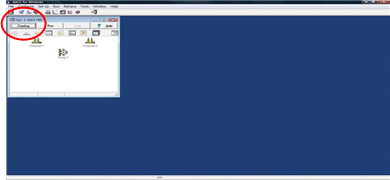
\includegraphics{E:/R/SOP/SOP_C07_TN/images/C07_image4_AACE 프로그램 실행 화면.png}

1.1.2.3. 시스템창의 Charting 버튼을 클릭하여 2항목(총질소, 총인)의 분석창이 뜨면서 장비가 작동한다.
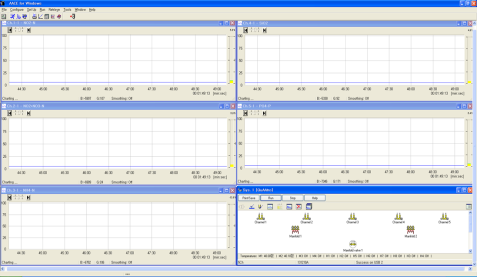
\includegraphics{E:/R/SOP/SOP_C07_TN/images/C07_image5_Charting 메뉴 각 항목 분석 화면.png}

1.1.2.4. 각 창에 마우스 커서를 두고 우클릭하여 총질소는 smoothing 4, 총인은 smoothing 12로 설정한다. 피크 정상부분이 평평하지 않으면 smoothing값을 높여 피크정상부분을 평형하게 하려는 시도가 종종 있으나 이는 권장하지 않는다. Smoothing 값을 크게 하면 분석 시 피크가 완만하게 상승하고 피크 정상 부분의 평평한 상태로 유지되는 시간이 짧아 피크가 뾰족한 모양으로 나와 안정된 분석값을 얻기 어렵다.

1.1.3. 기기세척 및 안정화
펌프의 시약튜브를 System Wash solution(5.1.4)(전처리 시약튜브는 증류수)에 담그고 sampler의 sample wash solution에 증류수를 연결하여 펌프를 작동시키면서 분석기기가 안정될 때까지 기다린다. 전처리장치의 온도가 110℃에 도달하는지, 컴프레셔의 압이 적절한지 확인한다. 안정화는 흡광도가 baseline이 ±0.1\% 범위내로 일정하게 유지되는 상태이다. 기기를 켠 후 안정화까지 약 1시간이 소요된다. baseline 값은 6\textasciitilde20\% 사이로 유지하고 이를 벗어날 경우 아래 9.2.2.1의 내용에 따라 baseline을 조정한다.

1.1.4. 시약 제조
1.1.4.1. 냉장고에서 standard stock(5.4.1)을 꺼내서 실온으로 맞춘다. 온도차이로 인해 피펫팅 시 부피가 변하지 않도록 일정한 온도를 유지하도록 노력한다.
1.1.4.2. 발색 시약제조법(5.2)을 참고하여 분석 전 혹은 분석 당일 발색시약을 제조하고, 5.4를 참고하여 5개 이상 농도구간의 총질소 표준용액을 만든다.

1.1.5. 시료의 준비
1.1.5.1. 냉동시료는 해동하는데 시간이 많이 소요되므로 해동하는 시점을 잘 정해야 한다. 분석기기가 준비되기 전에 미리 시료를 해동했는데 분석기기에 문제가 생기면 분석을 할 수 없어 해동한 시료의 처리가 곤란하기 때문에 적절한 시점에 녹여야 한다. 약 10 mL 시료의 경우 미온수에 1시간 이상 해동이 필요하고 50 mL 이상 용량의 시료는 2\textasciitilde3시간 이상 해동이 필요하다. 해동된 시료는 분석 전 상온에 보관하여 실온에 맞춘다.
1.1.5.2. 용존실리카의 경우 특수한 경우를 제외하면 24시간 이상 해동이 필요하므로 해동 한 다음 날 추가분석이 필요하다. 아래는 24시간 이상 해동이 필요하지 않은 시료의 조건이다(아래의 조건을 모두 충족해야한다).
- 용량 15 mL 이하
- 채수 직후 --80 ℃ 초저온 냉동 보관
- 보관 기간 한 달 이내

\hypertarget{uxbd84uxc11duxc900uxbe44-1}{%
\subsection{분석준비}\label{uxbd84uxc11duxc900uxbe44-1}}

1.2.1. TrAAcs 800 분석프로그램 (AACE) 분석파일 작성
1.2.1.1. Set up - Analysis - New analysis에서 새로운 Analysis file을 생성한다(아래 그림 참조).
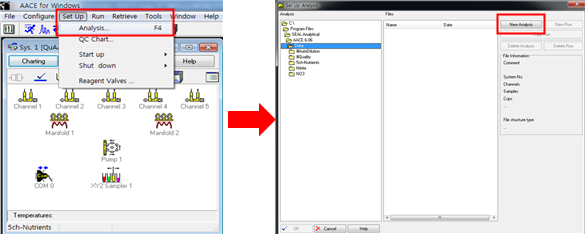
\includegraphics{E:/R/SOP/SOP_C07_TN/images/C07_image6_새로운 Analysis file 생성.png}

1.2.1.2. 위에서 New analysis 항목을 선택하게 되면 아래와 같이 Set Up: Analysis-new****.anl 창이 나타난다. 이 창에는 Main Page, Tray Protocol, Channel 1\textasciitilde2 탭들을 확인할 수 있다.
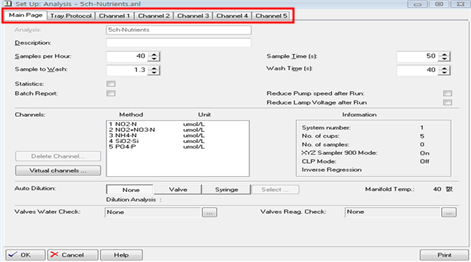
\includegraphics{E:/R/SOP/SOP_C07_TN/images/C07_image7_Main Page 탭 설정 화면.png}

1.2.1.3. Main Page : 각 채널들에 공통적으로 적용되는 항목을 설정하며 분석명과 Sample/Wash time을 설정할 수 있다. 한국해양과학기술원에서는 Sample/Wash time을 2분/2분로 설정하여 사용하고 있다. 이 시간을 변경하게 되면 peak 정상부분이 변형되는 ISAC현상이 나타날 수 있으니 변경 시에는 충분한 검토가 필요하다. Peak 정상부분에 ISAC현상이 일어날 경우에 대한 조치는 제조사에서 제공한 매뉴얼(부록4)을 참고하여 조치를 해야한다.

1.2.1.4. Tray Protocol : 분석 시 필요한 시료 목록을 작성한다.
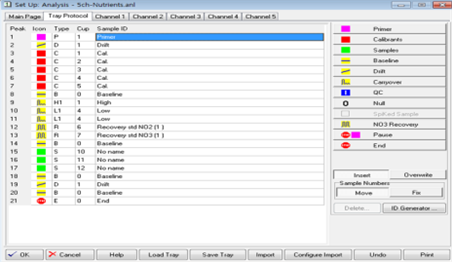
\includegraphics{E:/R/SOP/SOP_C07_TN/images/C07_image8_Tray Protocol 탭 시료 목록 작성 화면.png}

\begin{verbatim}
- primer: 분석기기의 시작을 위해 맨 처음 분석되는 시료로 분석기기의 운용 프로그램에서 primer를 peak로 인식해야만 그 후 분석하는 시료의 peak와 tray protocol에 입력한 분석 순서를 일치시킬 수 있다. primer의 peak 높이는 약 30%로 설정되어 있으며(분석기기 매뉴얼 권장 사항) 총질소와 총인 모두 포함되어있어야 한다. primer의 피크 높이는 main page에서 수정 가능하다. 

- calibrants: 농도계산에 사용될 검정곡선을 위한 표준용액열이다. 표준용액열의 최대 농도는 예상되는 시료의 최대 농도보다 높은 농도로 준비한다. Channel 탭(9.2.1.5)에 표준용액열의 농도를 입력하고 검량선 종류를 선택하면 프로그램에서 환산한 농도를 분석창에서 확인할 수 있다.

- drift: 분석 중 발색시약의 변화와 같은 분석 조건의 변화에 의한 시료 농도값 변화에 영향을 주는 것을 보정하기 위한 시료이다. 

- carry over: 앞에 분석된 고농도 또는 저농도 시료가 다음 시료에 미치는 영향을 보정하기 위한 것으로 high-low-low순서 또는 low-low-high 순으로 표준용액열의 가장 높은 농도와 가장 낮은 농도(‘0’값 제외)를 차례로 분석하게 하면 프로그램에서 자동적으로 보정할 수 있다. 이 순서는 검정곡선에 사용되는 표준용액열과 시료를 분석할 때 고농도에서 저농도 (high-low-low) 또는 저농도에서 고농도 (low-low-high)로 분석하느냐에 따라 다르게 사용된다.

- baseline: 미량의 영양염 분석을 위해 초순수를 baseline용액으로 이용한다. 초순수를 네 번 반복 분석하여 마지막 peak를 baseline으로 설정한다. 표준용액열 전 후, 인증 표준물질 전 후, 시료 약 20개 분석 전 후로 초순수를 분석하여 baseline을 주기적으로 분석한다. 또한 고농도 시료 분석 후 저농도 시료 분석 시 잔류영향(Carryover effect)를 제거하기 위해 초순수를 분석한다.

- Sample: 시료분석 순서는 저농도에서 고농도로 시료를 배치하고 정점과 정점 사이에 증류수를 분석하여 정점을 구분한다. 정점당 시료의 개수가 12개 미만이면 두 개 정점을 분석한 후에 drift를 넣어 이를 보정할 수도 있다. 분석할 시료수가 많으면, 검량선의 유효성을 확인하기 위해서 시료 20-24개마다 baseline(증류수)과 drift (primer)를 분석한다. Drifter의 평균회수율이 80~120%이면 시험에 사용된 검정곡선을 유효한 것으로 보며 그 변화된 값을 보정해준다 (drift correction). drift 시료는 두 번 이상 분석하여 마지막 결과를 사용하여 보정에 이용한다.
\end{verbatim}

\begin{itemize}
\item
  MDL시료: 제조사의 검출한계나 예상 검출한계의 5배의 농도로 결정된 시료(총질소 약 1.2μM, 총인 약 0.2μM). 방법검출한계 측정용 첨가시료로 매 분석 시 7번 반복 분석하여 방법검출한계 점검(8.7 방법검출한계 계산 방법 참고).
\item
  NO3 Recovery: 5μM로 농도가 동일한 NO2, NO3 용액을 매 분석마다 분석하여 카드뮴-구리 환원관의 환원효율을 점검하고 환원효율이 95\% 이하일 경우 충분히 환원되지 않았다고 판단되므로 카드뮴-구리 환원관을 교체한다.
\end{itemize}

\(환원효율= \frac{5\mu M ~ NO_{3} 분석결과}{5\mu M ~ NO_{2} 분석결과}~~~ \times 100\)(\%)

분석 전 환원용액의 결과를 알기 어렵기 때문에 총질소의 gain값 및 std A 표준용액의 peak 높이(\%)를 관찰해야한다. peak가 이전에 비해 낮아지고, gain이 높아졌다면 이전에 비해 환원율이 떨어졌다는 의미로 카드뮴-구리 환원관을 교체 후 시료를 분석해야한다.

\begin{itemize}
\item
  QC: 안정성이 뛰어난 물질 여러 종류를 매 분석마다 3번씩 반복 분석하여 분석 정밀도를 계산한다(8.2.3). 농도가 검증된 인증 표준물질을 이용할 경우 3번 반복 분석한 결과로 분석 정확도(8.2.2)를 계산하여 분석 품질을 평가하고 관리할 수 있다.
\item
  Cup: 시료를 sampler의 rack에 배치한 후 sampler rack의 번호를 입력하는 칸. cup 번호를 정확히 입력해야만 올바른 시료를 sampler가 흡입할 수 있다.
\end{itemize}

1.2.1.5. Channel : 각각의 channel을 선택하면 각 channel에 할당된 분석방법 (method), baseline, drift, carryover correction등의 실행 여부를 프로그램에서 자동적으로 선택할 수 있다. 검정곡선에 사용되는 용액의 농도(calibrants 1\textasciitilde10), 검정곡선 fitting의 종류, 신호의 순간적인 변동(noise)에 의한 오차를 줄이는 smoothing, peak determination window time 등을 설정한다. 총질소는 Smoothing 4, 총인은 smoothing 8로 설정한다. 각각에 대한 자세한 설명은 기기 매뉴얼을 참고한다.

\begin{figure}
\centering
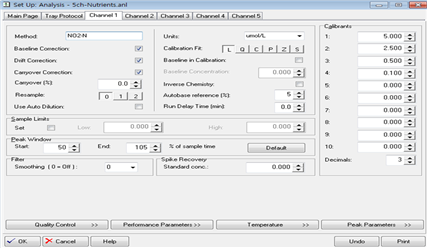
\includegraphics{E:/R/SOP/SOP_C07_TN/images/C07_image9_Channel 탭 설정 화면.png}
\caption{캡션을 입력하세요}
\end{figure}

1.2.1.6. 위의 창에서 채널별로 설정을 모두 완성한 후 OK를 클릭하면 Main 창의 analysis 칸에 기입한 이름(분석명.anl)으로 저장된다. 추후 분석 시 Set up - Analysis 항목에서 저장된 Analysis file을 선택하거나 위의 system 창 좌측하단 분석명이 있는 곳을 더블 클릭하여 기존에 작성된 파일에서 sample table 등을 포함한 기타 수정사항을 변경하여 사용한다.

1.2.2. 제조한 시약 연결 및 baseline 확인

1.2.2.1. 9.1.3의 상태에서 흡광도 값이 6\textasciitilde20\%를 벗어나면 시스템창의 channel버튼을 눌러 baseline을 수동으로 6\textasciitilde20\%사이에 위치하게 맞춘다(UPW baseline). 기기 내부 공기방울 패턴이 일정한지 확인한다.
1.2.2.2. System wash solution(wash triton-X, wash SDS, UPW)에 연결되어있던 시약튜브를 각 분석 항목별 시약 용기에 연결하여 기기가 안정되기를 기다린다.
1.2.2.3. Imidazole이 분석기기의 분석관에 들어간 것을 확인한 다음 카드뮴-구리 환원관 valve를 열어 시약 및 시료가 카드뮴-구리 환원관을 지나가도록 설정한다.
1.2.2.4. 산화용액 및 발색용액으로 인해 총질소, 총인 분석 채널의 baseline이 증가한다(Reagent blank, RB). baseline이 6\%\textasciitilde20\% 사이에 위치하도록 시스템창의 channel 1(총질소), channel 2(총인)를 더블클릭하여 baseline을 수동으로 조작한다.
1.2.2.5. Gain값 설정: 표준용액열 중 가장 농도가 높은 std A용액(총질소: 60 μM, 총인: 10μM)을 2분 동안 흡입하고 초순수를 2분 동안 흡입하는 과정을 세 번 반복한다. 약 20분 후 총질소와 총인의 peak가 분석창에 나타나면 시스템창의 channel을 열어 peak의 정상부분이 80\textasciitilde85\%에 위치하도록 gain을 수동으로 조절한다. baseline과 gain 설정은 분석 범위를 설정하기 위한 단계인 동시에 시약, 분석환경 등의 변화를 관찰할 방법으로 baseline과 gain값이 일정한지 지속적인 점검이 필요하다.

1.2.3. 시료 분석 시작 및 종료

1.2.3.1. 9.2.2의 전 과정이 끝나면 sample table에 작성한 시료 번호대로 rack(부록3 참고)에 시료를 꽂는다. rack holder에 rack을 정확히 꽂아야 sample probe가 정확히 시료를 찍을 수 있으니 유의해야한다.
1.2.3.2. 시스템창의 run을 누른 후 미리 준비 해둔 분석파일(9.2.1)을 선택한다.
1.2.3.3. 시료분석이 완료된 후 baseline이 안정화되어 분석창이 자동으로 꺼질 때까지 기다린다. 만약 마지막에 baseline 불안정하여 분석이 자동으로 종료되지 않으면 강제로 분석을 종료를 하고 재계산을 통해서 자료를 회수한다.

1.2.4. 분석종료 후 처리

1.2.4.1. 분석종료 후에는 카드뮴-구리 환원관 밸브를 닫고 컴프레셔와 전처리장비를 끈다. 시약에 꽂아두었던 시약튜브를 빼서 증류수를 담은 병에 꽂아 장비의 manifold를 세척한다.
1.2.4.2. 약 1시간 정도 씻은 후 시약튜브를 닦아 호일로 감싸 기기의 manifold속 용액을 모두 비운다.
1.2.4.3. 시스템창의 stop을 눌러 분석창을 닫은 후 분석기기와 sampler의 전원을 끄고 펌프덮개를 열어 펌프튜브의 손상을 방지한다.
1.2.4.4. 사용한 시약병/부피플라스크 등은 씻어 다음 분석 시 사용될 수 있도록 준비한다(세척순서 : 초순수 -- 10\% 염산 -- 초순수 3번 -- 건조).

\hypertarget{uxc790uxb8cc-uxbd84uxc11d-uxbc0f-uxacc4uxc0b0-2}{%
\section{자료 분석 및 계산}\label{uxc790uxb8cc-uxbd84uxc11d-uxbc0f-uxacc4uxc0b0-2}}

1.1. 분석이 완료되면 retrieve - view chart를 클릭하면 분석한 파일 이름을 선택할 수 있고 파일을 선택하면 아래 그림과 같이 피크가 나온다. 모든 분석결과에 대해 아래 빨간색 박스로 표시된 부분을 눌러 피크의 위치를 조정한다. 피크위치를 설정할 때는 peak window에서 일정한 위치를 선정하여 일관성을 유지하도록 한다. 박스안의 계산기 버튼을 눌러 농도를 재계산한다.
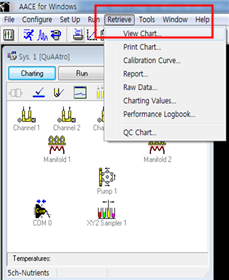
\includegraphics{E:/R/SOP/SOP_C07_TN/images/C07_image10_Retrieve_View Chart 이동.png}
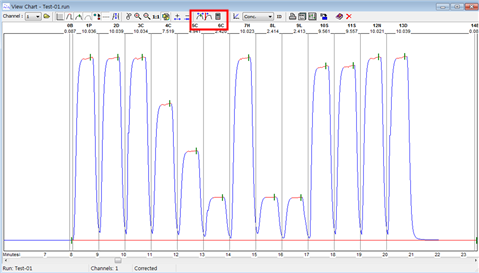
\includegraphics{E:/R/SOP/SOP_C07_TN/images/C07_image11_peak 위치 조정.png}
1.1. 엑셀을 이용하여 자료를 재계산할 경우 {[}file{]} - {[}export{]} - {[}ASCⅡ file{]} - chart를 선택 후, sylk format으로 내보낸다. 파일은 설정한 경로에 excel파일로 저장된다.
\includegraphics{E:/R/SOP/SOP_C07_TN/images/C07_image12_File_Export To 이동.png}
\includegraphics{E:/R/SOP/SOP_C07_TN/images/C07_image13_파일 형식 선택 저장.png}
1.1. 시료 분석값이 검량곡선에 사용된 가장 높은 표준용액열 보다 높은 경우 시료를 희석하여 재분석한다.

\hypertarget{uxcc38uxace0uxbb38uxd5cc-5}{%
\section{참고문헌}\label{uxcc38uxace0uxbb38uxd5cc-5}}

1.1. 김기동, 허미경, 서용찬, 총질소와 총인 수동 및 자동 분석의 비교평가(Ⅰ) - 총질소분석, 한국환경분석학회지, Vol. 9, No.~2, p.199-206, 2006.

1.2. 해양환경공정시험기준, 2021, p.97\textasciitilde104.

\hypertarget{uxbd80uxb85d-1.-uxc601uxc591uxc5fc-uxc790uxb3d9uxbd84uxc11duxae30traacs-800uxc758-uxc7a5uxbe44uxad6cuxc131uxacfc-uxae30uxb2a5}{%
\section{부록 1. 영양염 자동분석기(TrAAcs 800)의 장비구성과 기능}\label{uxbd80uxb85d-1.-uxc601uxc591uxc5fc-uxc790uxb3d9uxbd84uxc11duxae30traacs-800uxc758-uxc7a5uxbe44uxad6cuxc131uxacfc-uxae30uxb2a5}}

\hypertarget{uxce21uxc815uxc6d0uxb9ac-2}{%
\subsection{측정원리}\label{uxce21uxc815uxc6d0uxb9ac-2}}

연속흐름분석법(CFA, Continuous Flow Analysis)은, 분석관 내부에 일정량의 시약과 시료를 주입하고 공기를 규칙적으로 주입하여 분절하면서 시료와 시약을 잘 혼합하여 발색시켜 flowcell이 장착된 비식계로 흡광도를 측정하여 농도를 결정한다.

\hypertarget{uxc7a5uxbe44uxad6cuxc131-uxbc0f-uxae30uxb2a5-1}{%
\subsection{장비구성 및 기능}\label{uxc7a5uxbe44uxad6cuxc131-uxbc0f-uxae30uxb2a5-1}}

1.2.1 Console(콘솔, 본체)

\begin{figure}
\centering
\includegraphics{E:/R/SOP/SOP_C07_TN/images/C07_image14.png}
\caption{캡션을 입력하세요}
\end{figure}

1.2.2 펌프
2개의 proportional pump로 각각의 펌프는 시약 및 시료를 분석관에 주입 할 수 있는 튜브를 10개씩 부착한다. 각각의 펌프는 펌프튜브를 눌러주는 platen과 12개의 롤러로 구성되어 있고 펌프가 한 바퀴 회전하는데 12초가 걸린다.

1.2.3 펌프 튜브
1.2.3.1 분석항목에 따라 들어가는 시약의 양이 다르므로 튜브의 Flow rate를 조절하기 위해 각각 다른 튜브를 사용한다. 튜브의 굵기는 color code로 구분한다. 튜브별 flow rate와 color code는 아래 표에 정리되어 있다.
1.2.3.2 튜브의 굵기는 Color Code로 구분한다.
1.2.3.3 튜브 교체시기 : 분석항목과 시약에 따라 차이가 발생 할 수 있으나, 보통 운전 150\textasciitilde200시간마다 교체한다.

1.2.4 분석관(Manifold)
혼합코일, 카드뮴코일의 교환밸브 등으로 이루어져 있으며, 시료가 시약과 혼합이 되어 비색계로 들어간다.

1.2.5 비색계
1.2.5.1 30mm 길이의 Flow cell이 장착된 비색계가 기본 2대 장착되어 있으며 각각 550nm, 800nm에서 총질소, 총인을 분석한다.
1.2.5.2 또한 Software로 비색계의 감도(Gain) 및 Baseline을 조정할 수 있다.

\hypertarget{sampler-1}{%
\subsection{Sampler}\label{sampler-1}}

\begin{figure}
\centering
\includegraphics{E:/R/SOP/SOP_C07_TN/images/C07_image15.png}
\caption{캡션을 입력하세요}
\end{figure}

\hypertarget{uxc804uxcc98uxb9acuxc7a5uxbe44d2bx-02}{%
\subsection{전처리장비(D2BX-02)}\label{uxc804uxcc98uxb9acuxc7a5uxbe44d2bx-02}}

\begin{figure}
\centering
\includegraphics{E:/R/SOP/SOP_C07_TN/images/C07_image16_전처리장비.png}
\caption{캡션을 입력하세요}
\end{figure}

\hypertarget{compressure}{%
\subsection{compressure}\label{compressure}}

\begin{figure}
\centering
\includegraphics{E:/R/SOP/SOP_C07_TN/images/C07_image17_compressure.png}
\caption{캡션을 입력하세요}
\end{figure}

\hypertarget{uxbd80uxb85d-2.-flow-diagram-1}{%
\section{부록 2. Flow Diagram}\label{uxbd80uxb85d-2.-flow-diagram-1}}

\hypertarget{uxcd1duxc9c8uxc18c}{%
\subsection{총질소}\label{uxcd1duxc9c8uxc18c}}

\begin{figure}
\centering
\includegraphics{E:/R/SOP/SOP_C07_TN/images/C07_image18_총질소 Flow Diagram.png}
\caption{캡션을 입력하세요}
\end{figure}

\hypertarget{uxc804uxcc98uxb9acuxc7a5uxce58}{%
\subsection{전처리장치}\label{uxc804uxcc98uxb9acuxc7a5uxce58}}

\begin{figure}
\centering
\includegraphics{E:/R/SOP/SOP_C07_TN/images/C07_image19_전처리장치 Flow Diagram.png}
\caption{캡션을 입력하세요}
\end{figure}

\hypertarget{uxbd80uxb85d-3.-sample-rack-position-1}{%
\section{부록 3. Sample rack position}\label{uxbd80uxb85d-3.-sample-rack-position-1}}

\hypertarget{sample-rack-position-1}{%
\subsection{Sample rack position}\label{sample-rack-position-1}}

0은 분석 시 sample probe를 세척하고 시료와 시료 간 sample wash solution이 들어가는 부분이기 때문에 실제 시료 및 표준용액을 높는 위치는 1부터 시작한다.
\includegraphics{E:/R/SOP/SOP_C07_TN/images/C07_image20_Standard rack position_1.png}

\hypertarget{sample-rack-position-2}{%
\subsection{Sample rack position}\label{sample-rack-position-2}}

\begin{figure}
\centering
\includegraphics{E:/R/SOP/SOP_C07_TN/images/C07_image21_Standard rack position_2.png}
\caption{캡션을 입력하세요}
\end{figure}

\hypertarget{uxbd80uxb85d-4.-uxc2dcuxb8ccuxc0acuxc774-uxacf5uxae30uxc218uxcd95inter-sample-air-compression-isac-1}{%
\section{부록 4. 시료사이 공기수축(Inter Sample Air Compression, ISAC)}\label{uxbd80uxb85d-4.-uxc2dcuxb8ccuxc0acuxc774-uxacf5uxae30uxc218uxcd95inter-sample-air-compression-isac-1}}

시료 간 공기수축(ISAC)은 자동시료주입기에서 시료 흡입을 마친 후 다음 시료를 흡입 할 준비를 위해서 세척액으로 이동할 때, 그리고 세척을 마친후 다음 시료로 이동하는 동안 흡입된 공기방울이 펌프롤러에 눌리면서 시료주입 튜브 내 압력이 대기압과 유사하거나 약간 낮아져 발생하는 현상이다. 시료주입 튜브 내 압력이 감소하면서 눌려진 공기방울 앞쪽의 시료 흐름이 순간적으로 감소하고 시약과 혼합되는 시료의 부피가 감소된다. 결과적으로, 이러한 압력의 변화로 정상적일 때 보다 적은 양의 시료가 주입되어 농도가 낮은 구간이 발생한다.

\begin{figure}
\centering
\includegraphics{E:/R/SOP/SOP_C07_TN/images/C07_image22.png}
\caption{캡션을 입력하세요}
\end{figure}

따라서 긴 시료를 흡입 할 경우 다이어그램에 표시된 것처럼 시료피크 정상의 끝부분에서 피크가 움푹 파인 모양이 나타난다. 움푹 파인 정도가 크거나, 피크의 중간부분에 위치할 경우 분석결과의 정확도가 떨어진다. 이를 방지하기 위해 펌프와 시료주입 피팅 사이의 시료주입 튜브 의 길이를 조정하여 ISAC구간을 피크정상에서 벗어나 피크의 시작부분이나 끝부분에 위치하게끔 조절해야한다. ISAC구간을 계산하는 방법은 다음과 같다. 공기방울이 펌프를 지나 주입피팅에 도달하는데 걸리는 시간이 시료 당 분석 소요시간(시료주입+세척시간)보다 약 2\textasciitilde8초(목표는 3초) 짧아야한다.
현재 한국해양과학기술원에서 시간당 시료분석 개수는 60개이고, 자동 시료주입구의 시료와 세척의 시간 비는 3:1이다.
시료주입:45초
세척시간:15초
시료 당 분석 소요 시간: 60초\\
따라서 펌프와 주입피팅 사이의 이동 시간은 52\textasciitilde58초(목표는 57초)이다.

시료주입 튜브 길이조정 방법\\
가. 펌프에서 시료주입 피팅 사이의 시료주입 튜브의 길이를 충분히 길게 준비한다.
나. 기기를 동작시키고 시료 간 공기방울이 펌프를 지날 때 자세히 살핀다.
다. 공기방울이 펌프를 벗어나는 것이 보이는 순간은 공기방울이 펌프롤러를 지난 후 이미 2초 경과한 상태이다. 목표한 시간까지 계속 시간을 측정한다(시계가 없을 경우에는 공기밸브가 2초마다 작동하므로 이를 이용하여 시간을 측정할 수 있음). 목표로 한 시간에 공기방울 위치를 시료주입 튜브에 표시한다.
라. 펌프 동작을 멈추고 시료주입 튜브를 자르고 주입피팅에 연결한 뒤 펌프를 작동시킨다.
마. 만약 튜브의 적정 길이가 너무 짧아 주입피팅까지 도달하지 않으면 목표시간을 한 번 더 더해줄 수 있다.
Double ISAC = 목표시간 +시료주입시간+세척시간
= 57초 + 45초 + 15초 = 117초

\hypertarget{uxbd80uxb85d-5.-coating-procedure-of-cd-coil}{%
\section{부록 5. Coating Procedure of Cd coil}\label{uxbd80uxb85d-5.-coating-procedure-of-cd-coil}}

\hypertarget{uxce74uxb4dcuxbbb4uxd658uxc6d0uxad00-uxd65cuxc131uxc2dcuxc57d5.3-uxcc38uxace0}{%
\subsection{카드뮴환원관 활성시약(5.3 참고)}\label{uxce74uxb4dcuxbbb4uxd658uxc6d0uxad00-uxd65cuxc131uxc2dcuxc57d5.3-uxcc38uxace0}}

5.1.1 10\% Acetone
5.1.2 10\% HCl
5.1.3 2\% Copper sulfate
5.1.4 Imidazole buffer

\hypertarget{uxce74uxb4dcuxbbb4-uxd658uxc6d0-uxc808uxcc28}{%
\subsection{카드뮴 환원 절차}\label{uxce74uxb4dcuxbbb4-uxd658uxc6d0-uxc808uxcc28}}

5.2.1 50 mL 10\% HCl, 200 mL증류수를 비커에 담는다.
5.2.3 10 mL 주사기에 증류수를 넣어 카드뮴 코일에 연결하여 세척한다.
5.2.4. 10 mL 주사기에 염산을 넣어 카드뮴 코일에 연결하여 세척한다.
5.2.5. 위 과정을 염산 1번, 증류수 2번으로 카드뮴 코일에서 이물질이 나오지 않을 때 까지 반복 세척한다. 증류수나 염산으로 세척할 때 공기를 같이 불어 넣어주면 카드뮴 코일속의 이물질을 빨리 제거할 수 있다.
5.2.6 10 mL주사기에 Imidazole buffer 10 mL를 넣고 카드뮴 코일을 통과 시킨다.
5.2.7. 10 mL 주사기에 황산구리 용액을 가득채운 후 15분 동안 순차적으로 5 mL, 3 mL, 2 mL를 천천히 카드뮴 코일에 흘려준다. 이때 공기와 접촉하지 않도록 주의한다. 황산구리 용액을 너무 빨리 흘려주면 카드뮴과 황산 결합이 깨어진다.
5.2.9. 10 mL주사기에 Imidazole buffer 10 mL를 넣고 카드뮴 코일을 통과 시킨다. 최소 12시간 동안 보관 후에 사용한다.
5.2.10.새로 제작한 카드뮴 코일은 10\% 아세톤 원액을 12 mL를 주사기를 이용하여 천천히 흘려준 후 5.2.3부터 과정을 시작한다.

\hypertarget{uxc6a9uxc874uxc0b0uxc18c-uxbd84uxc11d-uxd45cuxc900uxc6b4uxc601uxc808uxcc28uxc11c}{%
\chapter{용존산소 분석 표준운영절차서}\label{uxc6a9uxc874uxc0b0uxc18c-uxbd84uxc11d-uxd45cuxc900uxc6b4uxc601uxc808uxcc28uxc11c}}

\hypertarget{uxbaa9uxc801-uxbc0f-uxbc94uxc704-5}{%
\section{목적 및 범위}\label{uxbaa9uxc801-uxbc0f-uxbc94uxc704-5}}

해수시료의 용존산소 측정은 해수에 녹아 있는 산소가 아이오다이드 이온(I\textsuperscript{-})을 트리아이오다이드(I\textsuperscript{3-})로 정량적으로 산화시킨 후 발생된 트리아이오다이드(I\textsuperscript{3-})를 티오황산염 용액으로 적정하여 화학적으로 정량화하는 Winkler(1888) 적정법을 기초로 Carpenter(1965)가 변경한 적정법을 사용한다. 이 표준운영절차서는 해양수산부의 해양환경공정시행법 (2013-230)에 기초하고 있으며, 종말점 결정에 전기화학적인 방법의 적용, 분광광도법의 적용방법이 추가되어 있다.

\hypertarget{uxce21uxc815-uxc6d0uxb9ac-3}{%
\section{측정 원리}\label{uxce21uxc815-uxc6d0uxb9ac-3}}

일정량의 해수시료에 염화망간(MnCl\textsubscript{2})을 첨가한 다음 곧 바로 알카리아오다이드화나트륨(NaOH/NaI)을 첨가하면 강한 알카리 환경에서 망간이온(Mn\textsuperscript{2+})은 수산화망간(Mn(OH)\textsubscript{2})으로 침전한다(식1). 이때 수산화망간은 해수시료속에 용존되어 있는 용존산소와 반응하여 수화된 4가의 망간산화물(MnO(OH)\textsubscript{2})의 갈색 침전물을 형성한다(식2). 시료병에 황산을 첨가하여 강한 산성환경을 만들어주면 갈색 침전물인 수화된 4가의 망간산화물(MnO(OH)\textsubscript{2})이 산화제로 작용하여 시료속에 첨가된 아오다이드이온(I\textsuperscript{-})을 아이오딘(I\textsubscript{2})으로 산화시킨다(식3). 이렇게 생성된 아이오딘(I\textsubscript{2})은 시료에 과잉으로 존재하는 아오다이드이온(I\textsuperscript{-})과 결합하여 트리아이오다이드 착물(I\textsuperscript{3-})을 형성한다(식4). 생성된 트리아이오다이드 착물을 티오황산나트륨 용액으로 정량하여 해수시료속에 존재하고 있는 용존산소 농도를 계산한다. 티오황산염은 트리아이오다이드 착물(I\textsuperscript{3-})을 아이오다이드이온(I\textsuperscript{-})으로 환원시키는 역할을 한다. 생성된 트라이아이오다이드 착물(I\textsuperscript{3-})을 아이오다이드이온(I\textsuperscript{-})으로 완전히 환원시키는데 사용된 티오황산염량은 생성된 트리아이오다이드 착물(I\textsuperscript{3-})량의 두배이다(식5). 종말점을 정밀하게 확인하기 위해서 적정이 완료되기 직전에 녹말용액을 첨가하면 아직 아이오다이드이온(I\textsuperscript{-})로 환원되지 않고 남아 있는 트리아이오다이드 착물(I\textsuperscript{3-})과 반응하여 푸른색을 띤다(식6). 푸른색이 사라지면 시료속의 트리아이오다이드 착물(I\textsuperscript{3-})이 완전히 아이오다이드이온(I\textsuperscript{-})으로 환원되었음를 의미한다. 그리고 2몰의 티오황산염이 1몰의 트리아이오다이드 착물(I\textsuperscript{3-})을 환원시키므로 이때까지 사용된 티오황산염의 1/2몰이 시료속의 존재했던 트리아이오다이드 착물(I\textsuperscript{3-})의 몰수이고, 이는 수환된 4간의 망간산화물(MnO(OH)\textsubscript{2})에서 생성된 1몰의 아이오딘(I\textsubscript{2})에 해당한다. 해수시료속의 용존산소(O\textsubscript{2}) 1몰은 2몰의 아이오딘(I\textsubscript{2})을 생성하므로 1몰의 아이오딘(I\textsubscript{2})은 해수시료의 용존산소(O\textsubscript{2}) 1/2몰에 해당한다. 따라서 해수시료중의 용존산소(O\textsubscript{2})는 트리아이오다이드 착물(I\textsuperscript{3-})을 아다이드이온(I\textsuperscript{-})으로 환원시키는 소비된 티오황산염량에 4를 곱하여 계산할 수 있다.

\begin{enumerate}
\def\labelenumi{(\arabic{enumi})}
\tightlist
\item
  \(Mn^{2+} + 2OH^{-} → Mn(OH)_{2}\)\\
\item
  \(2Mn(OH)_{2} + O_{2} → 2MnO(OH)_{2}\)\\
\item
  \(2Mn(OH)_{2} + 6H^{+} + 2I^{-} → 2Mn^{2+} + I_{2} + 6H_{2}O\)\\
\item
  \(I_{2} +I^{-} = I^{3-}\)\\
\item
  \(I^{3-} +{2S_{2}O_{3}}^{2-} → 3I^{-} +{S_{4}O_{6}}^{2-}\)\\
\item
  녹말 + \(I^{3-}\) → 푸른색
\end{enumerate}

이 방법으로 측정가능한 해수중 용존산소 법위는 0-400 μmol kg\textsuperscript{-1}이다. 이 방법의 정확도는 0.1\% 미만 또는 ±0.3 μmol kg\textsuperscript{-1}이다.

\hypertarget{uxbc29uxd574uxbb3c-3}{%
\section{방해물}\label{uxbc29uxd574uxbb3c-3}}

이 분석법은 \textbf{황화수소가 포함된 해수시료 분석}에는 부적합하다.

\hypertarget{uxae30uxad6c-uxbc0f-uxae30uxae30-3}{%
\section{기구 및 기기}\label{uxae30uxad6c-uxbc0f-uxae30uxae30-3}}

해수중 용존산소 분석에 필요한 기구 및 기기는 크게 시료채취기구(4.1), 적정기구(4.2)등이 있다. 실험에 사용되는 초자류를 10\%의 염산으로 세척한 후 초순수로 3회 헹구어 사용한다.

\hypertarget{uxc2dcuxb8ccuxcc44uxcde8-uxae30uxad6c}{%
\section{시료채취 기구}\label{uxc2dcuxb8ccuxcc44uxcde8-uxae30uxad6c}}

\hypertarget{uxc2dcuxb8ccuxbcd1}{%
\subsection{시료병}\label{uxc2dcuxb8ccuxbcd1}}

시료병의 목부분이 가늘어 아오다인의 증기가 빠져나가기 어렵게 되어 있으며 젓빚유리 마개를 가지 125 ml정도의 Pyrex병을 사용한다. 시료병과 두껑은 한쌍으로만 사용하고 부피보정을 실시한다. 병의 부피는 ±0.003 ml 정밀도로 측정한다.

\hypertarget{uxc2dcuxc57duxbd84uxc8fcuxae30uxc2dcuxc57duxbcd1}{%
\subsection{시약분주기/시약병}\label{uxc2dcuxc57duxbd84uxc8fcuxae30uxc2dcuxc57duxbcd1}}

정밀분주기 3개가 필요하다. 시약1(MnCl2), 시약2(NaI/NaOH), 시약3(Sulphuric Acid)용 분주기 3개는 1.0 ml를 ±0.02 ml정밀도로 분주할 수 있어야 한다. 시약2(NaI/NaOH)용 분주기는 유리에 붙기 때문에 항상 주의를 기울여야 하고, 장기간 사용하지 않을 때 완전히 세척/분해하여 보관한다. 시약병은 장기간의 항해기간동안 햇빛의 영향을 방지하기 위해 차광병 사용을 권장한다. 시약1(MnCl2)과 시약2(NaI/NaOH)용 시약병은 실험실과 시료채취장소에 반복적으로 옮겨 다녀야 하기 때문에 두 시약병을 운반하는 상자를 사용하는 것이 편리하다. 시약병은 사각형모양을 사용할 것을 권장한다.

\hypertarget{uxc2dcuxb8ccuxcc44uxcde8uxd29cuxbe0c}{%
\subsection{시료채취튜브}\label{uxc2dcuxb8ccuxcc44uxcde8uxd29cuxbe0c}}

시료채취기(Niskin bottle)에서 시료병으로 시료를 옮길 때 투명하고 튜브벽의 두께가 얇아 휘기쉬운 플라스틱 튜브(Tygon tube)를 사용한다. 튜브의 직경은 시료병에서 시료를 흘러넘치게 할 때 적당한 속도가 될수 있을 정도의 직경이어야 한다. 휘기쉬운 실리콘 튜브를 짧게 잘라 Tygon tube 끝에 연결하여 시료채취 튜브를 니스킨병의 시료채취 꼭지에 연결하는데 편리하다. 시료채취 튜브를 사용하지 않을 때는 초순수에 보관한다. 시료채취전에 가볍게 만져 튜브 내부를 충분히 적셔주어 시료채취시 공기방울이 튜브 내부에 갇히는 것을 방지한다.

\hypertarget{uxc804uxc790uxc628uxb3c4uxacc4}{%
\subsection{전자온도계}\label{uxc804uxc790uxc628uxb3c4uxacc4}}

시료채취시 시료채취 튜브와 함께 시료채취병에 넣어 시료의 온도를 0.1 oC단위로 측정할 수 있는 전자온도계를 사용한다. 이때 측정된 온도는 시료채취시 해수의 밀도를 계산하는데 사용하고 자료처리과정에서 용존산소 농도단위를 μmol L-1에서 μmol kg-1로 변환하는데 사용한다. 또한 이 온도는 시료가 목표 수심에서 채취된 것인지 판단하는데 유용한 지표이다.

\hypertarget{uxc815uxbc00uxc800uxc6b8}{%
\subsection{정밀저울}\label{uxc815uxbc00uxc800uxc6b8}}

저울용량은 300g이고 정밀도가 0.001g인 전자저울을 사용한다.

\hypertarget{uxc801uxc815uxae30uxad6c}{%
\section{적정기구}\label{uxc801uxc815uxae30uxad6c}}

\hypertarget{uxc801uxc815uxc870uxc815uxc7a5uxce58}{%
\subsection{적정조정장치}\label{uxc801uxc815uxc870uxc815uxc7a5uxce58}}

자동적정을 위해서 티오황산염을 분주하기 위한 전동뷰렛과 종말점을 흡광도, 전류, 전위차로 감지하는 장치와 컴퓨터를 연결하는 조정장치로 구성되어 있다.

\hypertarget{uxbdf0uxb81b}{%
\subsection{뷰렛}\label{uxbdf0uxb81b}}

티오황산염을 미량으로 정밀하게 분주할 수 있는 1 ml, 2 ml, 또는 5 ml 수동 또는 전동뷰렛을 사용한다. 정밀한 적정을 위해 가급적 유리뷰렛 대신 정밀한 자동뷰렛을 사용하도록 한다.(예; Metrohm사의 665 Dosimat burette, SCHOTT Instruments사의 TITRONICⓡ universal)

\hypertarget{uxcd08uxc815uxbc00-uxbd84uxc8fcuxae30}{%
\subsection{초정밀 분주기}\label{uxcd08uxc815uxbc00-uxbd84uxc8fcuxae30}}

바탕용액이나 표준용액열을 제조하기 위해서 요오드산칼륨(KIO3)을 1.0 ml 와 10.0 ml를 정밀하게 옮길 때 사용하는 초정밀 분주기이다. SOCOREX Calibrex 520 bottle-top 분주기가 이러한 목적에 적합하다. 이 분주기는 1-11 ml까지 0.25 ml간격으로 증가시킬 수 있다. 분주기는 자주 사용하는 부피에 대해서 주기적으로 보정하여야 하고 재현성은 ±0.002-0.005 ml이다. 이목적에 적합한 다른 분주기는 MetrohmTM 피스톤 뷰렛이다.

\hypertarget{uxc790uxc11duxad50uxbc18uxae30}{%
\subsection{자석교반기}\label{uxc790uxc11duxad50uxbc18uxae30}}

25mm 테프론 코팅 자석교반막대기와 자석교반기가 필요하다.

\hypertarget{uxc2a4uxd034uxc988uxbcd1}{%
\subsection{스퀴즈병}\label{uxc2a4uxd034uxc988uxbcd1}}

250 ml 용량정도의 플라스틱병으로 초순수를 담아 눌러서 소량 배출하여 적정시 세척에 사용된다.

\hypertarget{uxc2dcuxc57duxc81cuxc870-3}{%
\section{시약제조}\label{uxc2dcuxc57duxc81cuxc870-3}}

용존산소 분석에 사용되는 시약은 염화망간(5.1), 알칼리 요오드화나트륨용액(5.2), 황산용액(5.3), 녹말지시약(5.4), 티오황산나트륨(5.5). 요오드화칼륨(5.6)등이 있다.

\hypertarget{m-uxc5fcuxd654uxb9dduxac04mncl24h2ouxc6a9uxc561}{%
\subsection{\texorpdfstring{3M 염화망간(MnCl\textsubscript{2}·4H\textsubscript{2}O)용액}{3M 염화망간(MnCl2·4H2O)용액}}\label{m-uxc5fcuxd654uxb9dduxac04mncl24h2ouxc6a9uxc561}}

염화망간(MnCl\textsubscript{2}·4H\textsubscript{2}O) 600 g을 초순수 500-700 ml가 담긴 눈금이 있는 비이커에 넣어 잘 저어 녹인후 실험실 온도까지 식힌 후 초순수로 최종부피를 1000 mL로 맞추어 제작한다. 공경이 큰 유리섬유 여과지로 여과하여 혹시 있을 수 있는 입자물질을 제거한 후 플라스틱 용기에 넣어 보관한다. 시간이 촉박할 경우 자석교반막대와 자석교반기를 사용하여 제작하면 시간을 단축할수 있다. 시약제조시 안전도구(글러브, 고글)을 착용하고 퓸후드에서 제작해야 한다. 염화망간 대신 황산망간(MnSO\textsubscript{4}·4H\textsubscript{2}O) 480 g을 초순수에 녹여 최종부피를 1000 ml로 맞추어 사용해도 된다.

\hypertarget{uxc54cuxce7cuxb9ac-uxc694uxc624uxb4dcuxd654uxb098uxd2b8uxb968nainaoh-uxc6a9uxc561}{%
\subsection{알칼리 요오드화나트륨(NaI/NaOH) 용액}\label{uxc54cuxce7cuxb9ac-uxc694uxc624uxb4dcuxd654uxb098uxd2b8uxb968nainaoh-uxc6a9uxc561}}

수산화나트륨(NaOH) 320 g을 초순수 500 ml가 담긴 눈금이 있는 비이커에 녹인후 냉각시킨다. 필요에 따라서는 찬물이 담긴 통에 비이커를 넣어 빨리 냉각시킬 수 있다. 냉각이된 비이커에 요오드화나트륨(NaI) 600 g을 천천히 첨가하여 녹인후 냉각시키다. 시료중에 아질산질소가 많이 포함되어 있으면 아질산질소의 방해를 제거하기 위해 아자이드화나트륨(NaN\textsubscript{3}) 10 g을 첨가하여 녹인다. 실험실 온도로 충분히 식힌후 초순수를 첨가하여 1000 ml로 맞춘다. 이 시약은 공경이 큰 유리섬유 여과지로 여과하여 입자물질을 제거한 후 차광용기에 보관하여 햇빛에 의한 변질을 최소화해야 한다. 시약제조시 안전도구(글러브, 고글)을 착용하고 퓸후드에서 제작해야 한다.

\hypertarget{vv-uxd669uxc0b0uxc6a9uxc561h2so4}{%
\subsection{\texorpdfstring{50\% (v/v) 황산용액(H\textsubscript{2}SO\textsubscript{4})}{50\% (v/v) 황산용액(H2SO4)}}\label{vv-uxd669uxc0b0uxc6a9uxc561h2so4}}

진한 황산(H\textsubscript{2}SO\textsubscript{4}) 50 mL를 초순수에 1:1의 비율(초순수 50 ml에 진한 황산 50 ml를 첨가)로 혼합한다. 반드시 초순수를 먼저 정량플라스크에 담은 후 진한 황산 50 ml를 천천히 열을 식혀가면서 첨가하여야 한다. 실온으로 냉가한 다음 정량플라스크에서 100 mL 눈금까지 맞춘다. 시약제조시 안전도구(글러브, 고글)을 착용하고 퓸후드에서 제작해야 한다. 시약제조시 폭발의 위험성이 있으므로 초순수에 진한 황산을 첨가하는 순서를 반드시 지켜야 하고, 황산을 첨가할 때 천천히 하여야 한다.

\hypertarget{uxb179uxb9d0uxc9c0uxc2dcuxc57d-1}{%
\subsection{1\% 녹말지시약}\label{uxb179uxb9d0uxc9c0uxc2dcuxc57d-1}}

수용성 녹말 1 g을 초순수 50 mL에 혼합한 다음 용액이 투명해질 때까지 가열하여 완전히 녹인 다음 초순수를 첨가하여 정확히 100 mL로 맞춘다. 그리고 이 용액은 상온으로 냉각하여 사용한다. 냉장보관이 가능하나 1주일을 초과하지 않아야 하며, 만약 장기간 보관하여야 할 경우에는 포화 염화수은(Hg\textsubscript{2}I\textsubscript{2})을 소량 첨가하여 보관한다.

\hypertarget{n-uxd2f0uxc624uxd669uxc0b0uxb098uxd2b8uxb968na2s2o35h2o-uxc6a9uxc561}{%
\subsection{\texorpdfstring{0.025 N 티오황산나트륨(Na\textsubscript{2}S\textsubscript{2}O\textsubscript{3}·5H\textsubscript{2}O) 용액}{0.025 N 티오황산나트륨(Na2S2O3·5H2O) 용액}}\label{n-uxd2f0uxc624uxd669uxc0b0uxb098uxd2b8uxb968na2s2o35h2o-uxc6a9uxc561}}

티오황산나트륨(Na\textsubscript{2}S\textsubscript{2}O\textsubscript{3}·5H\textsubscript{2}O) 약 6.205 g을 취하여 일정량의 초순수에 녹인후 정확하게 1000 mL로 맞춘다. 하지만 티오황산나트륨 용액의 농도는 분석하려는 시료의 용존산소 농도를 적정하기에 충분할 정도로 제조되어야 한다. 그리고 적정에 사용되는 뷰렛의 부피도 고려하여야 한다. 만약 시료의 용존산소 농도가 최대 400 μmol kg\textsuperscript{-1}정도이고 적정에 사용되는 티오황산나트륨의 부피를 최대 2 ml이하로 하려고 한다면 티오황산나트륨 용액의 적정농도는 다음과 같이 구한다.

\[4 \times (C_{1} \times V_{1}) = C_{2} \times V_{2}\]\\
여기서,\\
\(C_{1}: [O_{2}]=400 \mu mol L^{-1}\)\\
\(V_{1}:\) 용존산소 시료병 부피 (10\% 추가) \(=14ml\)\\
\(C_{2}: [Na_{2}S_{2}O_{3}]\)\\
\(V_{1}:\) 뷰렛부피 (2ml)\\
4:1 몰 산소(\(O_{2}\))적정에 4몰 \(Na_{2}S_{2}O_{3}\) 소비\\
따라서,\\
\([Na_{2}S_{2}O_{3}]=\frac{400 \mu mol ~ L^{-1} \times 140ml \times 4}{2ml} \simeq 0.11M\)\\
\([Na~2~S~2~O~3~]=400 * 10^-6^ * 140 * 4 / Burette volume (2 ml) = 0.11M\)

티오황산나트륨(Na\textsubscript{2}S\textsubscript{2}O\textsubscript{3}·5H\textsubscript{2}O) 1몰은 248.17 g이므로 약 27.4 g을 녹여서 1000 ml로 맞추면 된다. 만약 무수티오황산나트륨(Na2S2O3)을 사용할 경우 1몰이 158.09 g이므로 약 17.4 g을 사용한다. 이유는 확실하지 않으나 시약제조후 2-5일동안 보관후 사용하면 바탕값과 검량선값의 일일 변화가 적어 시간을 절약할 수 있으며 1L 이상 만들어 사용하기를 추천한다.

\hypertarget{m-uxc694uxc624uxb4dcuxc0b0uxce7cuxb968-uxd45cuxc900uxc6a9uxc561kio30.0100-n}{%
\subsection{\texorpdfstring{0.001667 M 요오드산칼륨 표준용액(KIO\textsubscript{3},0.0100 N)}{0.001667 M 요오드산칼륨 표준용액(KIO3,0.0100 N)}}\label{m-uxc694uxc624uxb4dcuxc0b0uxce7cuxb968-uxd45cuxc900uxc6a9uxc561kio30.0100-n}}

요오드산칼륨 (KIO\textsubscript{3}) 약 0.5 g을 120℃에서 약 2시간 동안 건조시킨 후 데시케이터에서 방냉한다. 요오드산칼륨 0.3567g을 정확히 취하여 초순수에 녹여 정확히 1000 mL로 한다. 실험실 온도(tp)를 측정하여 기록한다. 측정된 용존산소 농도의 정확도는 이시약을 얼마나 정확하게 만드느냐에 절대적으로 영향을 받는다. 본 시약은 티오황산염의 표준화에 사용되어지므로 정확히 0.3567g을 취하지 못할 경우, 측정 되어진 무게 값으로부터 몰 농도를 정확하게 구하여 티오황산염 용액의 표준화에 사용하도록 한다.

\[M (몰농도) =\frac{1L에 첨가되어진 요오드산칼륨 무게}{요오드산칼륨 분자량(214.0g)}\]

\hypertarget{uxc2dcuxb8ccuxcc44uxcde8-1}{%
\section{시료채취}\label{uxc2dcuxb8ccuxcc44uxcde8-1}}

\hypertarget{uxc2dcuxb8ccuxcc44uxcde8-uxac1cuxc694}{%
\section{시료채취 개요}\label{uxc2dcuxb8ccuxcc44uxcde8-uxac1cuxc694}}

채수기로부터 용존산소 분석을 위한 시료의 채취는 시료채취기가 표면에 도착후 가능한 짧은 시간내에 이루어 져야 한다. 수심이 깊은 곳에서 채수된 시료는 채수시간이 오래되었기 때문에 깊은 수심에서 표층으로 이동하는 동안 압력과 온도변화의 영향이 크기 때문에 시료채취를 먼저 해야 한다. 이는 표층에 대기하는 동안 온도가 상승하여 해수에 용존된 기체가 빠져나와 용존산소의 손실이 있을 수 있기 때문이다. 기체 시료 분석에 사용되는 시료 채취순서는 빈공간의 영향정도, 시료수가 적거나, 분석비용이 비싸거나, 분석에 노력이 많이 들어가는 순서로 하는 경우가 일반적이다. 일반적으로 사용되는 기체 시료채취 순서는 CFCs, Helium, Noble gases(aragon and zenon), O\textsuperscript{17}, Oxygen, and pCO\textsubscript{2}순이다.

\hypertarget{uxc2dcuxb8ccuxcc44uxcde8uxc808uxcc28}{%
\section{시료채취절차}\label{uxc2dcuxb8ccuxcc44uxcde8uxc808uxcc28}}

\begin{enumerate}
\def\labelenumi{\arabic{enumi}.}
\tightlist
\item
  시료병과 뚜껑이 일치하도록 준비한다.
\item
  시료채취시 사용하는 고정시약이 위험하니 조심해서 취급해야 하므로 보호장구(글러브와 고글) 착용을 권장한다.
\item
  시료병을 반쯤 채워 헹구는 것을 두 번 반복하여 이전에 사용한 시약 잔류물을 완전히 제거한 후 시료를 흘러 넘치게한다.
\item
  시료를 시료채취병에 채수할 때 시료채취 튜브를 시료병의 바닥까지 담군다음 시료를 천천히 채워 와류 또는 공기방울 생성을 최소화시킨다. 시료튜브를 눌러서 시료의 흐름을 줄여서 시료채취 튜브내의 공기방울 생성을 최소화한다. 그리고 시료채취를 시작할 때 시료병을 약 45도로 기울이고 시료가 차오르면 점진적으로 수직으로 세우면 시료채취시 공기방울 형성을 줄일 수 있다. 시료병을 채우는 데 걸리는 시간의 2-3배 정도 시료를 흘러넘치게 한 후 시료병 끝까지 채운다. 아직 시료병의 뚜껑을 닫지 않는다.
\item
  시료를 채우고 흘러넘치는 동안에 전자온도계를 시료병에 담구어 시료채취시 온도를 측정한다. 이때 측정된 온도는 시료채취시 시료중 용존산소가 고정되는 시점의 해수시료 밀도를 결정하는데 사용한다. 그리고 수층에서 시료채취기가 채수할 때 기록된 현장 CTD온도보다 높을 수 있다.
\item
  시료병에 채수가 완료되면 고정시약이 있는 곳으로 바로 이동하여 고정시약 염화망간 1 ml를 주입하고 이어서 알칼리 요오드화나트륨 용액 1 ml를 주입하고 뚜껑을 닫고 90초간 잘 흔들어 준다. 고정시약을 분주할 때 분주기 끝부분을 깊숙이 넣고 시약을 천천히 주입한다. 이는 시약이 너무 많이 혼합되지 않고 시료병의 바닥에 도달하도록 하여 병 입구 쪽에서 반응이 일어나는 것을 최소화해야 한다. NaI/NaOH 용액은 끈적거리기 때문에 분주기를 끝까지 올려 멈춰서 시약이 완전히 분주 되도록 해야 하고 주기적으로 분주기를 해체하여 씻어주어야 한다.
\item
  시료병의 뚜껑을 닫을 때 공기방울이 갇히지 않도록 주의해야 한다. 첨가된 고정시약 2 ml에 해당하는 시료가 뚜껑을 닫을 때 유실되는데 계산시 이를 고려한다.
\item
  엄지로 뚜껑을 잘 고정하여 손목을 사용하여 시료병을 위아래로 뒤집어 흔들어 시료와 시약을 잘 혼합한다.
\item
  시약과 시료를 완전히 혼합한 후 뚜껑과 병목사이에 있는 빈 공간에 스퀴즈병에 있는 초순수를 채워 공기의 출입이 차단되도록 밀봉한다. 이 과정은 따뜻한 시료가 건조하고 시원한 연구선 실내에 보관되면 수축하여 시료병 내부로 외부의 공기가 들어갈 수 있는 틈이 생길 수 있는데 이를 차단하기 위해서이다.
\item
  시약을 혼합한 후 약 30분이 지나면 한 번 더 시료병을 흔들어 시료병에 있는 모든 산소가 고정시약과 반응한 것을 확인한다. 그리고 초순수로 뚜껑을 다시 밀봉해야 한다.
\item
  시료병을 보통 1시간 30분에서 2시간 동안 실험실 온도로 맞춘 후 분석한다. 그러나 사정이 여의치 않으면 뚜껑의 밀봉이 유지되면 수일 동안 보관하였다가 분석하여도 뚜렷한 용존산소 농도 변화가 없다.
\end{enumerate}

\hypertarget{uxc2dcuxd5d8uxbc29uxbc95-1}{%
\section{시험방법}\label{uxc2dcuxd5d8uxbc29uxbc95-1}}

\hypertarget{uxc2dcuxc57duxbc14uxd0d5uxce21uxc815}{%
\section{시약바탕측정}\label{uxc2dcuxc57duxbc14uxd0d5uxce21uxc815}}

\begin{enumerate}
\def\labelenumi{\arabic{enumi}.}
\tightlist
\item
  시료병에 초순수를 반쯤 채우고 교반 자석 막대를 넣고 교반을 시작한다.
\item
  정밀분주기로 요오드화칼륨(KIO\textsubscript{3}) 1 ml를 정확하게 넣고 혼합한다.
\item
  50 \% 황산 1ml를 넣고 혼합한다.
\item
  NaI/NaOH용액 1ml를 넣고 혼합한다.
\item
  MnCl\textsubscript{2}용액 1 ml를 넣고 혼합한다.
\item
  시료병에 초순수를 채운다
\item
  티오황산나튬 용액으로 종말점까지 정확하게 측정한다. 종말점이 지나지 않도록 한다. 종말점까지 사용된 티오황산나트륨 부피(V1)를 기록한다. 만약 일부 자동 적정기에서는 종말점을 지나 적정하는 것을 방지하기 어려울 경우 종말점을 V1으로 기록하고 최종적으로 첨가된 부피른 V3고 기록한다.
\item
  이미 적정이 완료된 시료병에 요오드화칼륨(KIO\textsubscript{3}) 1 ml를 정확하게 다시 넣고 적정하여 사용된 티오황산나트륨 부피(V2)를 기록한다.
\end{enumerate}

\hypertarget{uxd2f0uxc624uxd669uxc0b0uxb098uxd2b8uxb968uxc6a9uxc561-uxd45cuxc900uxd654uxd45cuxc815-by-carpenter-1965-method}{%
\section{티오황산나트륨용액 표준화(표정) by Carpenter (1965) method}\label{uxd2f0uxc624uxd669uxc0b0uxb098uxd2b8uxb968uxc6a9uxc561-uxd45cuxc900uxd654uxd45cuxc815-by-carpenter-1965-method}}

\begin{enumerate}
\def\labelenumi{\arabic{enumi}.}
\tightlist
\item
  티오황산나트륨의 표정은 향후 용존산소 분석을 수행할 온도와 유사한 온도조건에서 수행한다.
\item
  용존산소 시료병에 초순수를 반쯤 채우고 교반자석막대를 넣어 교반기로 섞어준다.
\item
  위의 용존산소 시료병에 정확히 10.0 ml 요오드산칼륨 (0.00167 M)를 옮겨 섞어준다.
\item
  50\% 황산 용액 1 ml를 넣고 섞어준다.
\item
  알카리 요오드화나트륨(NaI/NaOH) 용액 1 ml를 넣고 잘 혼합하여 준다. 이때 요오드 이온(I\textsuperscript{-})은 요오드산(IO\textsubscript{3}\textsuperscript{-})에 의해 환원되어 트리아이오다이드 착물(I\textsubscript{3}\textsuperscript{-})을 형성한다 (IO\textsubscript{3}\textsuperscript{-} + 8I\textsuperscript{-} + 6H\textsuperscript{+} → 3I\textsubscript{3}\textsuperscript{-} + 3H\textsubscript{2}O).
\item
  염화망간 1 ml를 넣고 섞어준다.
\item
  초순수를 용존산소 시료병의 목부분까지 채운다\\
\item
  티오황산나트륨으로 적정을 실시한다. 노란 색이 거의 사라질 때 약 1 ml 녹말 지시액을 넣어준다. 이 때 용액은 반드시 진한 청색 또는 보라색을 띠어야 한다. 보라색이 사라질 때까지 적정을 한다 (I\textsubscript{3}\textsuperscript{-} + 2S\textsubscript{2}O\textsubscript{3}\textsuperscript{2-} → 3I\textsuperscript{-} + S\textsubscript{4}O\textsubscript{6}\textsuperscript{2-}). 이 적정법에 대해서는 ± 0.03 ml 이내의 재현성을 확보해야 한다.
\item
  요오드산(IO\textsubscript{3}\textsuperscript{-}) 1몰은 최종적으로 티오황산염(S\textsubscript{2}O\textsubscript{3}\textsuperscript{2-}) 6몰과 반응하게 된다. 그러므로 아래 식에 의해 적정에 사용되어진 티오황산나트륨 용액의 부피로부터 정확한 티오황산나트륨 용액의 몰농도를 간단히 구할 수 있다. 일반적으로 4번 분석한 값의 평균값을 사용하도록 한다. 종말점은 0.3\%이내이어야 하고, 단위는 ml 또는 μl이고 Vstd로 기록한다.
\end{enumerate}

\[C_{Na_{2}S_{2}O_{3} \cdot 5H_{2}O} = \frac{C_{KIO_3} \times 10.0 \times 6}{V_{Na_{2}S_{2}O_{3} \cdot 5H_{2}O}}\]\\
\(C_{Na_{2}S_{2}O_{3} \cdot 5H_{2}O} : Na_{2}S_{2}O_{3} \cdot 5H_{2}O\) 의 몰 농도 (mole/L)\\
\(C_{KIO_3}: KIO_3\)의 몰농도 (mole/L)\\
\(V_{Na_{2}S_{2}O_{3} \cdot 5H_{2}O}: Na_{2}S_{2}O_{3} \cdot 5H_{2}O\)의 적정부피 (mL)

\hypertarget{uxac80uxb7c9uxc120-uxbc29uxbc95standard-curveuxc5d0-uxc758uxd55c-uxd2f0uxc624uxd669uxc0b0uxb098uxd2b8uxb968-uxd45cuxc900uxd654uxc640-uxc2dcuxc57duxbc14uxd0d5-uxce21uxc815}{%
\section{검량선 방법(Standard-curve)에 의한 티오황산나트륨 표준화와 시약바탕 측정}\label{uxac80uxb7c9uxc120-uxbc29uxbc95standard-curveuxc5d0-uxc758uxd55c-uxd2f0uxc624uxd669uxc0b0uxb098uxd2b8uxb968-uxd45cuxc900uxd654uxc640-uxc2dcuxc57duxbc14uxd0d5-uxce21uxc815}}

\begin{enumerate}
\def\labelenumi{\arabic{enumi}.}
\tightlist
\item
  요오드화칼륨(KIO\textsubscript{3}) 2, 4, 6, 8, 10 ml를 초순수가 반쯤 채워진 각각의 용존산소병에 넣어 5개의 표준용액열을 준비한다.
\item
  각 표준용액열을 적정하여 종말점을 기록한다.
\end{enumerate}

\hypertarget{uxc2dcuxb8ccuxbd84uxc11d-1}{%
\section{시료분석}\label{uxc2dcuxb8ccuxbd84uxc11d-1}}

\begin{enumerate}
\def\labelenumi{\arabic{enumi}.}
\tightlist
\item
  용존산소병 목부분에 부어둔 밀봉용 초순수를 버리고 킴와이프를 사용하여 남아있는 수분을 제거한다.
\item
  뚜껑을 제거하고 교반용 막대자석을 넣는다.
\item
  50\% 황산 1 ml를 넣고 교반기로 잘 혼합하여 침전물을 녹인다. 만약 침전물이 다 녹지 않으면 50\% 황산 1 ml를 추가한다. 황산의 추가가 pH가 낮아지면 산소가 시약과 반응하여 발생하는 아이오딘(I\textsubscript{2})의 생성이 더 이상 일어나지 않는다. 이는 혼합이나 적정시 용존산소병에서 발생하는 기포는 더 이상 용존산소 측정에 영향을 주지 않는다는 의미이다.
\item
  티오황산나트륨 용액의 온도(t\textsubscript{L})을 기록한다.
\item
  시료를 종말점까지 적정하여 종말점을 기록한다. 적정부피의 단위가 ml인지 ul인지 확이하여 Vsam으로 기록한다.
\item
  시료병을 세척하여 시약잔류물을 제거한다. 굳이 초수수수로 세척하지 않아도 무방하다.
\end{enumerate}

\hypertarget{uxacc4uxc0b0}{%
\section{계산}\label{uxacc4uxc0b0}}

\hypertarget{uxc2dcuxc57duxbc14uxd0d5uxac12}{%
\section{시약바탕값}\label{uxc2dcuxc57duxbc14uxd0d5uxac12}}

시료에 있는 산화 또는 환원 불순물로 인해서 I\textsubscript{2}를 생성하기 때문에 시약바탕은 시료속에 있는 용존산소와 상관없이 나타났다.\\
V\textsubscript{blk} = V\textsubscript{1}-V\textsubscript{2}\\
적정기가 종말점을 지나서 멈추었다면\\
V\textsubscript{blk} = V\textsubscript{1}-(V\textsubscript{2}-(V\textsubscript{3}-1)) = 2V\textsubscript{1}-V\textsubscript{2}-V\textsubscript{3}\\
V\textsubscript{1}: 첫 번째 KIO3 1 ml를 적정한데 사용된 티오황산나트륨 용액의 부피\\
V\textsubscript{2}: 첫 번째 종말점 후 추가된 KIO\textsubscript{3} 1 ml를 종말점까지 적정한데 소모된 티오황산나트륨 용액의 부피\\
V\textsubscript{3}: 첫 번째 KIO\textsubscript{3} 1 ml를 적정할 때 종말점을 지났을 때 까지 사용된 티오황산나트륨 용액의 부피\\
V\textsubscript{blk}의 단위는 ml이다.

\hypertarget{kio3uxc758-uxb18duxb3c4-uxbcf4uxc815}{%
\section{\texorpdfstring{KIO\textsubscript{3}의 농도 보정}{KIO3의 농도 보정}}\label{kio3uxc758-uxb18duxb3c4-uxbcf4uxc815}}

KIO\textsubscript{3}를 제조할 때 온도(t\textsubscript{p})에서 농도를 온도가 20 ℃일 때 KIO\textsubscript{3}의 농도로 보정해야하고 방법은 아래와 같다.

\[M(KIO_{3}, ~ 20^{\circ} \mathrm C)= \frac {m(KIO_{3})/(213.995g \cdot mol^{-1})}{V_{s}} \times \frac{0.998206}{\rho _{w} (t_{p})}\]\\
\(m(KIO_{3}):\)부피플라스크에 들어있는 \(KIO_3\)의 질량\\
\(V_{s}:\) \(KIO_3\)를 제조할 때 온도(\(t_{p}\))에서 용액의 부피\\
\(213.995g~mol^{-1} : KIO_3\) 1몰의 질량\\
\(\rho_{w} (t_{p}):\) 용액이 제조될 때 실험실 온도에서 물의 밀도\\
\(V_{s} = V_{s}[1+\alpha_{V} (t_{L} -20)]\)\\
\(\alpha_{V}\)(Pyrex유리의 부피팽창계수)\(: 9.75 \times 10^{-6} ~^{\circ} K^{-1}\)

\hypertarget{uxd2f0uxc624uxd669uxc0b0uxb098uxd2b8uxb968-uxbab0uxb18duxb3c4}{%
\section{티오황산나트륨 몰농도}\label{uxd2f0uxc624uxd669uxc0b0uxb098uxd2b8uxb968-uxbab0uxb18duxb3c4}}

실온(tL)에서 티오황산나트륨 용액의 몰농도는 아래식으로 계산한다.

\[M(Na_{2}S_{2}O_{3}, ~ t_{L})= \frac{6000 \times V(KIO_{3}, ~ t_{L}) \times M(KIO_{3}, ~ t_{L})}{V_{std} - V_{blk}}\]\\
여기서,\\
\(V(KIO_{3}, ~ t_{L}) = V(KIO_{3}, ~ 20^{\circ} \mathrm C) \times (1+9.75 \times 10^{-6} (t_{L} -20))\)\\
\(M(KIO_{3}, ~ t_{L}) = M(KIO_{3}, ~ 20^{\circ} \mathrm C) \times \frac{\rho_{W} (t_{L})}{0.998206}\)\\
\(6000 = \frac{6mol~Na_{2}S_{2}O_{3}}{1mol~ KIO_{3}} \times \frac{1000 \mu l}{1ml}\)\\
\(V_{std}\):\(KIO_3\) 용액을 적정하는데 사용된 티오황산나트륨 용액의 평균부피\\
\(V_{blk}\): 시약바탕(reagent blank)으로 단위는 ml 또는 μl이다.

\hypertarget{uxd574uxc218uxc2dcuxb8ccuxc758-uxc0b0uxc18cuxb18duxb3c4}{%
\section{해수시료의 산소농도}\label{uxd574uxc218uxc2dcuxb8ccuxc758-uxc0b0uxc18cuxb18duxb3c4}}

적정된 산소 총몰수(시료+시약에 녹아있는 O\textsubscript{2})는 다음 식으로 계산된다.\\
\[n(O_{2})=(V_{sam}-V_{blk}) \times M(Na_{2}S_{2}O_{3}, ~ t_{L}) \times \frac{1L}{10^{6} \mu l} \times \frac{1 mol ~ O_2}{4 mol ~ Na_{2}S_{2} O_{3}}\]\\
\[C(O_2)= \frac {[n(O_2)-7.6 \times 10^{-8}]}{m(sample)}\]\\
여기서,\\
\(7.6×10^{8}\) : 시약(\(MnCl_2\) + \(NaI/NaOH\)) 2 ml에 들어 있는 용존산소(\(O_2\))의 양\\
\(m(sample)\)은 해수시료의 질량(kg)으로 다음식으로 계산한다.\\
\(m(sample)=V(O_{2} 시료병, ~ 20^{\circ} \mathrm C) \times [1 + 9.75 \times 10^{-6} (t_s - 20)]-2 \times \rho (t_S), ~ S)\)\\
여기서,\\
\(t_S\)는 시료채취시간의 온도\\
2 는 첨가된 고정시약부피로 인한 해수시료 손실\\
\(\rho_{SW}\)는 시료채취시점의 밀도

\hypertarget{uxc815uxb3c4uxd3c9uxac00uxc815uxb3c4uxad00uxb9acqaqc-1}{%
\section{정도평가/정도관리(QA/QC)}\label{uxc815uxb3c4uxd3c9uxac00uxc815uxb3c4uxad00uxb9acqaqc-1}}

자료의 정밀도를 향상시키기 위해 주기적으로 같은 채수기에서 5 ∼ 10 개 시료를 받아 분석해 보는 것이 좋다. 이 때 정밀도는 0.44 μmol/L 이하로 분석되어야 한다. 현장 정밀도는 바다날씨에 따라 0.16 ∼ 0.94 μmol/L 사이로 변할 수 있다. 용존산소 측정용 시료는 앞서 언급한 것과 같이 즉시 분석해야 정도관리에 도움이 된다.\\
장기간의 분석동안 여러개의 요오드산 칼륨이 사용되었다면 동일한 티오황산나트륨 용액으로 측정한 요오드산칼륨 용액의 농도가 ±0.1 \%이어야 하고, 시약바탕값의 변화를 점검하고 용존산소가 동일한 수심에서 여러개의 시료를 채취하여 분석한 정밀도가 ±0.45 μmol kg\textsuperscript{-1}이내인지 확인한다.\\
용존산소 측정용 절대 표준물질은 없다. 판매용 제품은 실험실에서 새로 만든 표준물질과 비교하는데 유용하다. 표준물질은 상대적으로 안정하므로 값이 이상할 경우 적정기의 이상으로 진단할 수 있다. 중복 시료 사이의 값의 차이가 1.78 μmol/L보다 크다면 자료를 면밀하게 검토해야 한다. 특히 심층수 값이라면 이 전의 자료와 대비시켜 보아야 한다. 적정 자료는 CTD 산소센서 자료와 비교해 볼 수 있다. CTD 산소센서 자료는 연속 자료라는 장점이 있다.

\hypertarget{uxbd84uxc11duxc808uxcc28-uxd750uxb984uxb3c4-1}{%
\section{분석절차 흐름도}\label{uxbd84uxc11duxc808uxcc28-uxd750uxb984uxb3c4-1}}

\hypertarget{chlorophyll-a-uxbd84uxc11d-uxd45cuxc900uxc6b4uxc601uxc808uxcc28uxc11c}{%
\chapter{chlorophyll a 분석 표준운영절차서}\label{chlorophyll-a-uxbd84uxc11d-uxd45cuxc900uxc6b4uxc601uxc808uxcc28uxc11c}}

\hypertarget{uxbaa9uxc801-uxbc0f-uxbc94uxc704-6}{%
\section{목적 및 범위}\label{uxbaa9uxc801-uxbc0f-uxbc94uxc704-6}}

식물플랑크톤의 광합성 색소는 chlorophyll a, b, c 와 여러 보조색소로 구성되어 있다. 이 중 chlorophyll a 는 모든 식물플랑크톤에 포함되어 있기 때문에 식물플랑크톤의 생체량을 가장 잘 평가할 수 있는 장점이 있다. 식물플랑크톤의 현존량(생체량, 생물량)을 클로로필양으로 측정하는데는 분광광도계나 (터너) 형광분광광도계를 사용한다.

\hypertarget{uxce21uxc815-uxc6d0uxb9ac-4}{%
\section{측정 원리}\label{uxce21uxc815-uxc6d0uxb9ac-4}}

\hypertarget{uxbd84uxad11uxad11uxb3c4uxacc4uxc5d0-uxc758uxd55c-uxce21uxc815}{%
\subsection{분광광도계에 의한 측정}\label{uxbd84uxad11uxad11uxb3c4uxacc4uxc5d0-uxc758uxd55c-uxce21uxc815}}

식물플랑크톤의 광합성 색소를 90 \% 아세톤용액으로 추출하고 추출액의 흡광도를 750, 665, 645, 630, 480nm 에서 측정하여 chlorophyll a, b, c 및 총 카로티노이드 (total carotenoids) 량을 계산한다.
해수중 광합성 색소인 chlorophyll a 의 검출한계는 0.02μg/L이고, 그 이외 색소들의 검출 한계는 0.04μg/L 이다.
정밀도는 chlorophyll a 의 경우 5μg/L 농도수준에서 ± 0.3 μg/L, chlorophyll b 의 경우 0.5μg/L농도 수준에서 ± 0.2 μg/L이다.

\hypertarget{uxd130uxb108-uxd615uxad11uxbd84uxad11uxad11uxb3c4uxacc4uxc5d0-uxc758uxd55c-uxce21uxc815}{%
\subsection{터너 형광분광광도계에 의한 측정}\label{uxd130uxb108-uxd615uxad11uxbd84uxad11uxad11uxb3c4uxacc4uxc5d0-uxc758uxd55c-uxce21uxc815}}

이 방법은 아세톤으로 추출된 chlorophyll을 터너 형광광도계를 이용하여 측정하는 방법으로 분광광도계로 측정하는 방법보다 5\textasciitilde10배 감도가 높기 때문에 연안의 경우 100\textasciitilde200mL 정도의 시료만으로도 chlorophyll a 와 phaeo-pigment의 정량이 가능하다. 측정의 정밀도는 chlorophyll a의 농도 5 μg/L에서 ± 10 \% 이내이다.

\hypertarget{uxd615uxad11uxbd84uxad11uxad11uxb3c4uxacc4uxc5d0-uxc758uxd55c-uxce21uxc815}{%
\subsection{형광분광광도계에 의한 측정}\label{uxd615uxad11uxbd84uxad11uxad11uxb3c4uxacc4uxc5d0-uxc758uxd55c-uxce21uxc815}}

이 방법은 아세톤으로 추출된 chlorophyll을 형광광도계를 이용하여 여기파장 (exiting wavelength) 436nm, 형광파장 (emission wavelength) 670nm 에서 형광을 측정하여 chlorophyll a 와 phaeo-pigment를 측정하는 방법이다. 측정의 정밀도는 chlorophyll a 의 농도 5μg/L에서 ± 10 \% 이내이다.

\hypertarget{uxbc29uxd574uxbb3c-4}{%
\section{방해물}\label{uxbc29uxd574uxbb3c-4}}

광합성 색소인 chlorophyll a, b, c의 추출용액은 광분해가 쉽게 일어나기 때문에 여과 등의 실험과정에서 직사광선을 피해야 한다. 750nm 는 시료 중의 현탁물질에 의한 탁도 정도를 알기 위한 흡광도이다. 분광광도계의 측정 파장을 정확하게 맞추지 않으면 오차가 크게 발생한다.

\hypertarget{uxae30uxad6c-uxbc0f-uxae30uxae30-4}{%
\section{기구 및 기기}\label{uxae30uxad6c-uxbc0f-uxae30uxae30-4}}

해수중 총질소 분석에는 필요한 기구 및 기기는 여과기(4.1), 유리섬유여과지(4.2), 원심분리기(4.3), 마개 있는 원심분리관 또는 시험관 (보통 15mL)(4.4), 교반기(4.5), 분광광도계 측정법으로 분석하는 경우 분광광도계(4.6), 터너형 형광광도계 측정법으로 분석하는 경우 터너 형광광도계(4.7), 형광분광광도계 측정법으로 분석하는 경우 형광분광광도계(4.8)과 스크루 형 주사기(4.9), 스크루 형 filter holder(4.10) 등이 있다.

\hypertarget{uxc5ecuxacfcuxae30}{%
\subsection{여과기}\label{uxc5ecuxacfcuxae30}}

해수시료 중 식물플랑크톤을 여과지에 모으기 위한 여과기

\hypertarget{uxc720uxb9acuxc12cuxc720-uxc5ecuxacfcuxc9c0}{%
\subsection{유리섬유 여과지}\label{uxc720uxb9acuxc12cuxc720-uxc5ecuxacfcuxc9c0}}

해수시료 중 식물플랑크톤을 거르기 위한 유리섬유 여과지로 보통의 경우 GF/F, 47mm 를 사용한다.

\hypertarget{uxc6d0uxc2ecuxbd84uxb9acuxae30}{%
\subsection{원심분리기}\label{uxc6d0uxc2ecuxbd84uxb9acuxae30}}

여과지에 걸러진 엽록소 a를 아세톤 용매에 추출한 뒤 광학측정기에 사용할 상등액을 만드는 데 사용한다.

\hypertarget{uxc6d0uxc2ec-uxbd84uxb9acuxad00-uxb610uxb294-uxc2dcuxd5d8uxad00}{%
\subsection{원심 분리관 또는 시험관}\label{uxc6d0uxc2ec-uxbd84uxb9acuxad00-uxb610uxb294-uxc2dcuxd5d8uxad00}}

식물플랑크톤이 걸리진 여과지를 아세톤 용매에 추출하고, 상등액을 만들기 위해 원심분리하는 용기로 사용한다. 마개 있는 원심 분리관 또는 시험관으로 보통 15 mL를사용한다.

\hypertarget{uxad50uxbc18uxae30}{%
\subsection{교반기}\label{uxad50uxbc18uxae30}}

여과지의 식물플랑크톤 색소를 용매에 추출하기 위해 사용한다.

\hypertarget{uxbd84uxad11uxad11uxb3c4uxacc4spectrophotometer}{%
\subsection{분광광도계(spectrophotometer)}\label{uxbd84uxad11uxad11uxb3c4uxacc4spectrophotometer}}

분광광도계 측정법 사용시 480nm, 630nm, 645nm, 665nm, 750nm 흡광도 측정이 가능한 분광광도계로 1cm cell을 사용한다.

\hypertarget{uxd130uxb108-uxd615uxad11uxbd84uxad11uxad11uxb3c4uxacc4turner-10au}{%
\subsection{터너 형광분광광도계(Turner 10AU)}\label{uxd130uxb108-uxd615uxad11uxbd84uxad11uxad11uxb3c4uxacc4turner-10au}}

터너 형광분광광도계 측정법 사용시 터너 디자인 형광광도계에 F4T4-BL 램프, Wratten 47 B 또는 Corning CS 5-60 filter, Corning CS 2-64 filter가 있는 제품을 사용한다.

\hypertarget{uxd615uxad11uxbd84uxad11uxad11uxb3c4uxacc4spectrofluorometer}{%
\subsection{형광분광광도계(spectrofluorometer)}\label{uxd615uxad11uxbd84uxad11uxad11uxb3c4uxacc4spectrofluorometer}}

형광분광광도계 측정법 사용시 436nm 에서 여기파장(exciting wavelength), 670nm 에서 형광파장(emission wavelength) 측정이 가능한 형광분광광도계로 1cm 사각 cell을 사용한다.

\hypertarget{uxc2a4uxd06cuxb8e8-uxd615-uxc8fcuxc0acuxae30}{%
\subsection{스크루 형 주사기}\label{uxc2a4uxd06cuxb8e8-uxd615-uxc8fcuxc0acuxae30}}

분광광도법보다 적은 양의 시료 여과로 엽록소 a 측정이 가능한 형광분광광도계를 사용하는 경우 50mL 스크루 형 주사기를 시료여과에 사용한다.

\hypertarget{uxc2a4uxd06cuxb8e8-uxd615-filter-holder}{%
\subsection{스크루 형 filter holder}\label{uxc2a4uxd06cuxb8e8-uxd615-filter-holder}}

분광광보법보다 적은 양의 시료 여과로 엽록소 a 측정이 가능한 형광분광광도계를 사용하는 경우 25mm 여과지를 사용할 수 있는 스크루형 filter holder가 필요하다.

\hypertarget{uxc2dcuxc57duxc81cuxc870-4}{%
\section{시약제조}\label{uxc2dcuxc57duxc81cuxc870-4}}

엽록소 a 분석에 사용되는 시약은 아세톤(5.1), 탄산마그네슘 용액(5.2), 염산용액(5.3, 5.4), 플로레신 나트륨 용액(5.5) 등 이다.

\hypertarget{uxc544uxc138uxd1a4vv}{%
\subsection{90\% 아세톤(v/v)}\label{uxc544uxc138uxd1a4vv}}

1000mL 플라스크에 증류수 100mL와 분석용 아세톤 900mL를 넣어 만든다. 보관시에는 마개를 잘 막고 어두운 곳에 보관한다.

\hypertarget{uxd0c4uxc0b0uxb9c8uxadf8uxb124uxc298-uxc6a9uxc561}{%
\subsection{1\% 탄산마그네슘 용액}\label{uxd0c4uxc0b0uxb9c8uxadf8uxb124uxc298-uxc6a9uxc561}}

탄산마그네슘(MgCO\textsubscript{3}) 1g을 증류수 100mL에 첨가하고 잘 흔들어 만든다.

\hypertarget{uxc5fcuxc0b0uxc6a9uxc561}{%
\subsection{1:1 염산용액}\label{uxc5fcuxc0b0uxc6a9uxc561}}

터너 형광광도계 측정시 사용하는 시약으로 진한 염산 50 mL를 증류수로 희석하여 100mL로 만든다.

\hypertarget{n-uxc5fcuxc0b0uxc6a9uxc561}{%
\subsection{0.5 N 염산용액}\label{n-uxc5fcuxc0b0uxc6a9uxc561}}

형광분광광도계 측정시 사용하는 시약으로 진한 염산 (37\%) 41mL를 증류수로 희석하여 1000mL로 만든다.

\hypertarget{ppm-uxd50cuxb85cuxb808uxc2e0-uxb098uxd2b8uxb968-uxd45cuxc900uxc6a9uxc561}{%
\subsection{100 ppm 플로레신 나트륨 표준용액}\label{ppm-uxd50cuxb85cuxb808uxc2e0-uxb098uxd2b8uxb968-uxd45cuxc900uxc6a9uxc561}}

형광분광광도계 측정시 사용하는 시약으로 100mg 의 플로레신 나트륨(C\textsubscript{20}H\textsubscript{10}O\textsubscript{4}Na\textsubscript{2}, sodium fluorescein)을 초순수에 녹여 1L로 만들어 냉암소에 보관한다. 이 용액은 사용직전에 홀 피펫을 사용 정확히 1mL를 취하여 100mL로 만든다.

\hypertarget{uxc815uxb3c4uxad00uxb9acuxc6a9-uxd45cuxc900uxbb3cuxc9c8reference-material-rm}{%
\subsection{정도관리용 표준물질(Reference Material, RM)}\label{uxc815uxb3c4uxad00uxb9acuxc6a9-uxd45cuxc900uxbb3cuxc9c8reference-material-rm}}

Sigma Aldrich, Fluka 등에서 판매하는 색소 표준물질

\hypertarget{uxc2dcuxb8ccuxcc44uxcde8-uxbc0f-uxad00uxb9ac-1}{%
\section{시료채취 및 관리}\label{uxc2dcuxb8ccuxcc44uxcde8-uxbc0f-uxad00uxb9ac-1}}

분광광도계를 사용하는 경우, 동물플랑크톤을 제거하기 위해 약 0.3 mm 매쉬 정도의 나일론 네트를 장착시킨 여과세트에 해수시료 0.5에서 5,000 mL(해역에 따라 적당량을 취함)를 유리섬유 여과지로 여과한다.형광분광광도계를 사용하는 경우, 식물플랑크톤의 현존량이 높은 연안역이나 내만해역의 해수시료 100~200 mL를 정확히 취하여 여과기 또는 스크루형 주사기와 fiter holder를 이용하여 유리섬유여지 (GF/F, 직경 25mm)에 여과한다.

시료를 유리섬유 여과지로 여과하는 동안 1 \% 탄산마그네슘 용액 수 방울을 첨가한다. 그러나 첨가한 탄산마그네슘 용액이 시료의 산성화를 막는 완충제의 역할은 하더라도 색소파괴를 방지하는 효과가 확인되지 않아 탄산마그네슘 완충용액의 첨가는 생략하여도 무방하다.

물기가 제거된 여과지는 15mL 시험관 또는 원심분리관에 잘 접어 넣는다.

만일 곧바로 분석이 불가능할 경우는 빛을 차단하고 냉동보관 한다 (가능한 한 낮은 온도(-196℃ 혹은 -80℃의 낮은 온도)를 권장, 불가피 할 경우 -20℃ 가량의 일반 냉동고 사용가능). 80일 이내 분석을 권장한다.

\hypertarget{uxc2dcuxd5d8uxbc29uxbc95-2}{%
\section{시험방법}\label{uxc2dcuxd5d8uxbc29uxbc95-2}}

\hypertarget{uxbc14uxd0d5uxc6a9uxc561uxc758-uxd761uxad11uxb3c4-uxce21uxc815}{%
\subsection{바탕용액의 흡광도 측정}\label{uxbc14uxd0d5uxc6a9uxc561uxc758-uxd761uxad11uxb3c4-uxce21uxc815}}

7.1.1. 분광광도계 Cell-to-Cell Blank 보정 : 먼저 바탕용액 값은 분광광도계의 두 cell에 90 \% 아세톤용액을 채우고 Reference cell에 대한 시료 cell의 Cell-to-Cell blank를 750 nm, 665 nm, 645 nm, 630 nm, 480 nm에서 흡광도를 측정하여 다음과 같이 모든 E값을 보정한다.\\
\[E_{665}=OD_{665} - OD_{750}\\
E_{645}=OD_{645} - OD_{750}\\
E_{630}=OD_{630} - OD_{750}\]
여기에서 \(OD\)는 광학 흡광도 (optical density)임.

7.1.2. 분광광도계 표탁도 Blank의 측정 : 유리섬유여과지를 사용할 경우 빛의 흡수가 없는 것으로 알려진 파장 750 nm의 파장에서 E값을 읽는다. 이때 E값은 매우 낮으며, 이때의 Blank 값은 매우 적어 때때로 음의 값을 나타내기도 하지만 그 이유는 뚜렷하지 않다. 그 값이 음․양 어느 경우이든 ±0.002를 초과해서는 안되며, Cell-to- Cell Balnk 보정 후 모든 파장에서 E값에 사용한다.\\
Membrane 여과지를 사용할 경우 소량의 콜로이드 물질이 원심분리 후에도 남는 경우가 있다. 이때 이들 물질에 의한 E값은 사용하는 파장에 따라 변하며 빛의 산란효과에 의해 파장이 짧아질 때는 증가한다. Blank 값은 750nm에서 Cell-to-Cell Blank 값으로 보정하여 얻어진 E값 (E\textsubscript{b})를 아래의 f계수를 곱하면 탁도 Blank 값이 된다.\\
f = 1 (파장, 666, 645, 630nm)\\
f = 2 (파장, 510nm)\\
f = 3 (파장, 480nm)

따라서, 총 Blank 값은 Cell-to-Cell Blank 값과 탁도 Blank (f x Eb)를 합한 것이 된다. 식으로 표현하면 다음과 같다.\\
\[Total\,Blank = (Cell-to-Cell Blank) + (f \times E_b)\]

7.1.3. 터너 형광광도계 0점 조정: 바탕용액인 90 \% 아세톤으로서 형광광도계의 눈금을 0 에 맞춘다.

\hypertarget{uxc2dcuxb8ccuxbd84uxc11d-2}{%
\subsection{시료분석}\label{uxc2dcuxb8ccuxbd84uxc11d-2}}

7.2.1. 분광광도계를 사용하는 경우, 유리섬유 여과지가 끼워진 여과기에 해수시료 적당량을 따라 부으면서 여과시킨다.\\
여과압은 대기압의 1/2이하(진공펌프 사용시 진공압 20mm-Hg 이하)로 하여 여과지 위에 수분이 남아 있지 않도록 한다.\\
여과시 1\% 탄산나트륨 용액 수 방울 (3\textasciitilde5방울)을 해수에 첨가한다\textbf{(하지만 생략하여도 무방하다)}.\\
(터너) 형광분광광도계를 사용하는 경우, 유리섬유 여과지가 끼워진 여과기 또는 스크루형 주사기에 직경 25mm 용 스크루형 filter holder를 끼우고 해수시료 100\textasciitilde200mL 정도의 적당량을 따라 부으면서 여과시킨다. 여과압은 대기압의 1/2이하로 하여 여과지 위에 수분이 남아 있지 않도록 한다. 여과시 1\% 탄산마그네슘 용액 수 방울 (3\textasciitilde5)을 해수에 첨가한다\textbf{(하지만 생략하여도 무방하다)}.
7.2.2. 수분이 제거된 여과지는 다음의 과정을 거치거나 필요시 chlorophyll 추출을 위하여 냉장보관 한다.
7.2.3. 여과지를 원심분리관 또는 시험관에 넣고 90\% 아세톤 수용액을 15mL(분광광도계) 혹은 10mL(형광분광광도계)를 첨가한 후 교반기로 강하게 교반한 다음 하루동안 4℃이하의 냉암소에 보관한다.\\
7.2.4. 원심분리관 또는 시험관을 실온에서 10분간 (3,000\textasciitilde4,000 rpm) 원심분리 시킨다.\\
7.2.5. 측정\\
7.2.5.1 분광광도계: 원심분리한 후 상등액의 일부를 취하여 1cm 셀에 옮겨 750nm, 665nm, 645nm, 630nm, 480nm의 파장에서 흡광도를 측정한다.\\
7.2.5.2 터너 형광광도계: 원심분리한 시료의 상등액 일부를 취하여 측정 셀로 옮기고 시료의 형광광도계의 형광을 읽는다 (R\textsubscript{B}). 그리고 나서 5\% 염산용액 2~3 방울을 측정 셀에 떨어뜨리고 셀을 2~3회 위 아래로 뒤집어 혼합한 다음 형광광도계에 다시 셀을 넣고 형광을 읽는다 (R\textsubscript{A}). 이때 라운드 셀의 형광 빛이 통과하는 부분에 이 물질이 묻지 않도록 주의한다.\\
7.2.5.3 형광분광광도계: 시료 측정을 위해서 여기파장 436nm, 형광파장 670nm에 맞춘다. 우선 원심분리한 시료 용액을 소량취하여 1cm 사각 셀에 넣고 형광를 측정한다 (F\textsubscript{B}). 그 다음에 0.5N 염산용액 2\textasciitilde3 방울을 첨가하고 혼합이 완전히 이루어져 형광이 안정될 때까지 기다린 후 형광을 측정한다 (F\textsubscript{A}). 염산을 첨가하지 않는 시료를 측정할 때는 이전 시료의 염산이 셀에 남아 있지 않도록 주의하여야만 하며 측정하고자하는 시료 추출 용액 1\textasciitilde2 mL로 셀을 1\textasciitilde2회 헹구어 주는 것이 좋다.

\hypertarget{uxc5fduxb85duxc18c-uxb18duxb3c4-uxacc4uxc0b0}{%
\subsection{엽록소 농도 계산}\label{uxc5fduxb85duxc18c-uxb18duxb3c4-uxacc4uxc0b0}}

7.4.1. 분광광도계: 측정된 흡광도를 엽록소 농도(μg/L)로 환산한다.
\[Chlorophyll\;a, b, c (μg/L)=\frac{C_{a,b,c} \times v}{V} \times 1000\]
\(Chlorophyll\;a, b, c\) : 엽록소 a, b, c의 농도 (μg/L)\\
\(v\) : 추출한 아세톤의 양(mL)\\
\(V\) : 여과한 해수의 량(mL)\\
\(C_a\) : 11.6 E\textsubscript{665} - 1.31 E\textsubscript{645} - 0.14 E\textsubscript{630}(엽록소 a)\\
\(C_b\) : 20.7 E\textsubscript{645} - 4.34 E\textsubscript{665} - 4.42 E\textsubscript{630}(엽록소 b)\\
\(C_c\) : 55 E\textsubscript{630} - 1.31 E\textsubscript{665} - 0.14 E\textsubscript{645}(엽록소 c)

7.4.2. 분광광도계: 농도 계산에 사용된 모든 자료를 제시한다.\\
① 표준물질 농도\\
② 각 파장별 흡광도

7.4.3. 터너 형광광도계: 측정된 형광값으로 엽록소 농도(μg/L)로 환산한다.
\[Chlorophyll\;a(μg/L)=F_D\frac{r}{r-1}(R_B-R_A) \times 1000\]
\[Phaeo-pigment(μg/L)=F_D\frac{r}{r-1}(rR_A-R_B) \times 1000\]

\(F_D\) : door의 계수\\
\(r\) : 검량선에서 얻어진 비\\
\(R_B\) : 산을 첨가하기 전 형광광도계의 형광을 읽은 값\\
\(R_A\) : 산을 첨가하고 난 후 형광광도계의 형광을 읽은 값

7.4.4. 형광분광광도계: 측정 흡광도로 색소 농도는 다음과 같이 계산한다.
\[Chlorophyll\;a(μg/L)=\frac{(F_B-F_A)v}{F_{ph}(R-1)V}\]
\[Phaeo-pigment(μg/L)=\frac{R(F_A-F_b)v}{F_{ph}(R-1)V}\]
\(R\) : F\textsubscript{ch}/F\textsubscript{ph} (F\textsubscript{ch} 및 F\textsubscript{ph}는 각각 chlorophyll a 및 phaeo-pigment 고유형광)은 순수한 chlorophyll a의 F\textsubscript{B}/F\textsubscript{A} 값\\
\(v\) : 90\% 아세톤으로 추출한 부피(mL)\\
\(V\) : 여과한 해수의 부피(mL)

\hypertarget{uxd130uxb108-uxd615uxad11uxad11uxb3c4uxacc4-uxac80uxb7c9uxc120}{%
\subsection{터너 형광광도계 검량선}\label{uxd130uxb108-uxd615uxad11uxad11uxb3c4uxacc4-uxac80uxb7c9uxc120}}

7.5.1. 순수한 chlorophyll a를 얻는 것은 매우 어렵기 때문에 해양 식물플랑크톤으로부터 추출하여야만 한다. 이 방법은 전적으로 chlorophyll a만을 분석하도록 설치되어져 있지만 다른 chlorophyll에도 약간의 반응과 변화를 보인다. 이 때문에 식물플랑크톤의 종과 종과 사이에 약간의 차이가 있다. 건강하게 배양된 \emph{Skeletonema costatum} 또는 \emph{Skeletonema costatum}과 같은 양 (chlorophyll로서)의 \emph{Coccolithus huxleyii} 및 \emph{Peridinium trochoidium}로 혼합되어진 것을 chlorophyll source로 권장한다. 만약 그러한 배양을 이용할 수 없다면, phaeo-pigment 량이 불확실한 것을 제외하면 자연적인 식물플랑크톤의 개체군을 이용할 수 있다. 부영양화된 해역의 초기 ``bloom'' 상태(대수 생장기)인 표층수를 채수하여 이용한다.그러나 일정한 품질이 유지되는 표준시료의 확보가 어려운 경우, Sigma Aldrich, Fluka 등의 시약 제조사에서 판매하는 색소 표준물질을 활용할 수 있다.

7.5.2.충분히 배양된 또는 자연적인 개체군 50 mL를 여과하여 90\%으로 추출한다. 아세톤으로 추출한 용액을 형광광도계의 door 3에서 50에 맞춘다 (R\textsubscript{3}). 분광광도계의 파장 정열을 주의 깊게 맞추어 chlorophyll a를 측정한 후, 다음 식으로부터 door 3에 대한 F\textsubscript{3} 값을 측정한다.\\
\[F_3=\frac{C_a}{R_3}\]
알고있는 chlorophyll a의 새로운 값으로서 door 10과 30에서 50 이상이 되도록 90 \% 아세톤으로서 추출한 것을 희석한다. 위에서 아날로그로 표현된 것으로부터 F\textsubscript{10}과 F\textsubscript{30}을 계산한다.

7.5.3. Door의 계수 F\textsubscript{D}는 7.5.1 과 7.5.2.에서 얻어진 것과 동일하고, 같은 방법으로 구하여 진다. 비 r은 phaeo-pigment가 거의 없는 것으로부터 구하여진 R\textsubscript{B}/R\textsubscript{A} 값으로서 표준화를 위해서 사용된 추출액이다. 비 값은 2.2 가깝다.

\hypertarget{uxd615uxad11uxbd84uxad11uxad11uxb3c4uxacc4-uxc870uxc815}{%
\subsection{형광분광광도계 조정}\label{uxd615uxad11uxbd84uxad11uxad11uxb3c4uxacc4-uxc870uxc815}}

형광분광광도계의 감도를 ×1에 맞추고, 여기파장 (exciting wavelength) 436 nm, 형광파장 (emission wavelength) 670 nm로 맞추고 플로레신 나트륨 (C\textsubscript{20}H\textsubscript{10}O\textsubscript{4}Na\textsubscript{2}, sodium fluorescein) 표준용액 1 ppm의 형광을 100에 조정한다 (플로레신 나트륨 표준용액 0.5 ppm을 사용할 경우 여기파장 436 nm, 형광파장 515 nm에서 형광을 100이 되도록 조정한다).

\hypertarget{uxc815uxb3c4uxd3c9uxac00uxc815uxb3c4uxad00uxb9acqaqc-2}{%
\section{정도평가/정도관리(QA/QC)}\label{uxc815uxb3c4uxd3c9uxac00uxc815uxb3c4uxad00uxb9acqaqc-2}}

\hypertarget{uxbd84uxc11duxc808uxcc28-uxd750uxb984uxb3c4-2}{%
\section{분석절차 흐름도}\label{uxbd84uxc11duxc808uxcc28-uxd750uxb984uxb3c4-2}}

\hypertarget{uxc6a9uxc874uxc720uxae30uxd0c4uxc18c-uxbd84uxc11d-uxd45cuxc900uxc6b4uxc601uxc808uxcc28uxc11c}{%
\chapter{용존유기탄소 분석 표준운영절차서}\label{uxc6a9uxc874uxc720uxae30uxd0c4uxc18c-uxbd84uxc11d-uxd45cuxc900uxc6b4uxc601uxc808uxcc28uxc11c}}

\hypertarget{uxbaa9uxc801-uxbc0f-uxbc94uxc704-7}{%
\section{목적 및 범위}\label{uxbaa9uxc801-uxbc0f-uxbc94uxc704-7}}

용존유기탄소의 분석은 여과된 해수 시료 중에 용존되어 있는 유기물을 금속 촉매를 이용한 고온 연소장치로 완전히 산화시킬 때 발생하는이산화탄소(CO\textsubscript{2})의 양을 비분산형 적외선 감지기(NDIR)로 측정하여 용존유기탄소량으로 나타내는 원리이다. 이때 시료 중의 용존무기탄소는 산처리하여 질소기체로 에 의해 제거된다. 이 표준운영절차서는 해양수산부의 해양환경공정시행법 (2013-230)에 기초하고 있으며, 분석기기 준비 및 안정화, 표준물질 분석을 통한 품질관리도 작성이 추가되어 있다. 이 방법으로 측정 가능한 해수중 용존유기탄소 검출한계는 99\% 신뢰구간에서 0.05 mgC/L(4.16 μmolC/L)이다. 이 방법의 정밀도는 5 mgC/L(462.2 μM)에서 ±0.08 mg C/L(6.66 μM)이다.

\hypertarget{uxce21uxc815-uxc6d0uxb9ac-5}{%
\section{측정 원리}\label{uxce21uxc815-uxc6d0uxb9ac-5}}

주사기로 산성화된 시료를 자동 시료주입기에 있는 시료를 흡입하여 이산화탄소가 없는 기체를 이용하여 시료 속에 있는 이산화탄소를 제거한다. 이 시료를 촉매로 채워진 연소관에 주입하고 연소관 온도를 섭씨 680도까지 가열하여 시료 중의 유기탄소를 분해하여 산소로 산화시켜 이산화탄소로 전환하여 기체의 수분과 염소를 제거하여 NDIR 검출기로 이산화탄소를 측정하여 시료속의 용존 유기물을 정량화한다.
현재 다양한 회사에서 고온촉매산화법(High-Temperature Catalytic Oxidation, HTCO)을 사용하는 분석기기를 상업용으로 개발하였으며, 기본 구성은 아래 다이아그램에 있는 Shimadzu사의 HTCO 분석기기와 유사하다. 다만 제조사에 따라 미세한 차이는 있을 수 있다.

\begin{figure}
\centering
\includegraphics{E:/R/SOP/SOP_C11_DOC_HTCO/images/C11_image1_고온촉매 산화 분석기기의 분석흐름도.png}
\caption{캡션을 입력하세요}
\end{figure}

\hypertarget{uxbc29uxd574uxbb3c-5}{%
\section{방해물}\label{uxbc29uxd574uxbb3c-5}}

이 분석법에 사용된 NDIR 검출기는 기체속의 수분과 염소 성분에 민감하나 제습기와 할로겐 제거기로 이들 성분을 제거하기 때문에 특별한 방해요인은 없다.

\hypertarget{uxae30uxad6c-uxbc0f-uxae30uxae30-5}{%
\section{기구 및 기기}\label{uxae30uxad6c-uxbc0f-uxae30uxae30-5}}

해수중 용존유기탄소 분석에 필요한 기구 및 기기는 크게 시료채취기구(4.1), 여과기구(4.2), 전자저울(4.3)등이 있다. 실험에 사용되는 초자류를 10\%의 염산으로 세척한 후 초순수로 3회 헹구어 사용한다.

\hypertarget{uxc2dcuxb8ccuxcc44uxcde8-uxae30uxad6c-1}{%
\subsection{시료채취 기구}\label{uxc2dcuxb8ccuxcc44uxcde8-uxae30uxad6c-1}}

1.1.1. 시료채취기
수층 해수시료는 Go-Flo 채수기 또는 내부에 Teflon으로 코팅되어 있고 Teflon 코팅된 용수철이 있는 Niskin 채수병을 사용한다. 시료 채취기는 실리콘 튜브와 O-ring을 사용하여 밀폐한다. 채수기에 연결된 로프는 monofilament nylon 또는 Kevlar lanyard 재질의 줄을 사용하여야 한다.
1.1.2. 시료병
시료 채취에는 10ml 유리앰퓰 또는 자동 시료 주입기용 40ml 유리 바이알을 사용한다. Polycarbonate 재질의 시료병을 사용할 수 있다.

1.1.3. 시료 채취 튜브
시료 채취 튜브 없이 채수기의 꼭지에서 시료병으로 직접 채취하는 것을 권장한다.

\hypertarget{uxc5ecuxacfcuxae30uxad6c}{%
\subsection{여과기구}\label{uxc5ecuxacfcuxae30uxad6c}}

여과가 필요한 시료의 경우에는 PP, PE, Teflon재질의 25/47mm 여과기를 10\% 염산에 담군 후 초순수로 씻은 다음 시료 채취기 꼭지에서 직접 중력으로 여과하는 것을 권장한다. 시료 채취기와 여과기 사이의 연결은 PP, PE, Teflon 재질의 튜브를 가능한 짧게 하여 사용한다.

\hypertarget{uxc815uxbc00uxc800uxc6b8-1}{%
\subsection{정밀저울}\label{uxc815uxbc00uxc800uxc6b8-1}}

저울 용량은 300g이고 정밀도가 0.001g인 전자저울을 사용한다.

\hypertarget{uxbd84uxc11duxae30uxae30-2}{%
\subsection{분석기기}\label{uxbd84uxc11duxae30uxae30-2}}

1.4.1. 자동시료주입기
자동시료 주입기는 24mL vial\emph{93 ea, 9ml vial}93 ea, 40mL*68 ea

1.4.2. 연소기
680도까지 가열할 수 있음

1.4.3. 연소관
백금촉매로 구성되어 있음

1.4.4. 비분산 적외선 감지기(NDIR detector)

1.4.5. 스퀴즈병
250 ml 용량정도의 플라스틱병으로 초순수를 담아 눌러서 소량 배출하여 적정시 세척에 사용된다.

\hypertarget{uxc2dcuxc57duxc81cuxc870-5}{%
\section{시약제조}\label{uxc2dcuxc57duxc81cuxc870-5}}

용존유기탄소 분석에 사용되는 시약은 저탄소수(5.1), 표준용액(5.2), 산화효율측정 용액(5.3), 운반기체(5.4)등이 있다. 표준용액열 제조에 사용되는 초자는 부피 측정의 정확도에 문제가 발생하지 않도록 고온으로 연소하지 않고 10\% 염산에 24시간 이상 담근 후 초순수로 씻어 알루미늄 호일로 입구를 막아 섭씨 100도 이하에서 건조하여 준비한다.

\hypertarget{uxc800uxd0c4uxc18cuxc218low-carbon-water-lcw}{%
\subsection{저탄소수(Low-Carbon Water, LCW)}\label{uxc800uxd0c4uxc18cuxc218low-carbon-water-lcw}}

일반적으로 저탄소수 제조에 Milli-Q시스템이 사용된다. 주기적으로 품질을 확인하여야 한다. 저탄소 수는 기기 바탕 값 측정, 현장 바탕값 및 표준용액 원액, 표준용액열 희석, 산화 효율측정 원액 및 작업용 산화 효율측정 표준액 제조에 사용된다.

\hypertarget{uxc720uxae30uxd0c4uxc18c-uxc6d0uxc56183.3-mmolcl}{%
\subsection{유기탄소 원액(83.3 mmolC/L)}\label{uxc720uxae30uxd0c4uxc18c-uxc6d0uxc56183.3-mmolcl}}

미리세척한 비이커에 Potassium Hydrogen Phthalate(potassium biphthalate, C\textsubscript{8}H\textsubscript{5}KO\textsubscript{4}, 204.22g/mol) 약 2.5g을 넣고 깨끗한 오븐에서 섭씨 100도로 4시간 정도 건조하여 수분을 제거한 후 데시케이터에서 상온으로 냉각한다. 2.1254g을 취해서 700mL의 LCW에 녹인 다음 최종 부피를 1000mL로 맞춘다.
작업용 표준용액열은 유기탄소 원액 일정량을 취해서 LCW로 희석하여 맞추고 진한 인산을 첨가하여(약 4 μl H\textsubscript{3}PO\textsubscript{4}/mL) pH를 2\textasciitilde3 정도로 맞춘다.

\hypertarget{uxc0b0uxd654uxd6a8uxc728uxce21uxc815-uxc6a9uxc561oxidation-effiency-check-stock-solution-oec}{%
\subsection{산화효율측정 용액(Oxidation Effiency Check Stock Solution, OEC)}\label{uxc0b0uxd654uxd6a8uxc728uxce21uxc815-uxc6a9uxc561oxidation-effiency-check-stock-solution-oec}}

산화효율측정 원액을 제조하기 위해서 Sulfathiazole(C\textsubscript{9}H\textsubscript{9}N\textsubscript{3}O\textsubscript{2}S\textsubscript{2}, 255.31g/mol) 약 2.8g과 EDTA(C\textsubscript{10}H\textsubscript{16}N\textsubscript{2}O\textsubscript{8}, 292.2438g/mol) 약 2.8g을 각각의 미리 씻은 비커에 넣고 깨끗한 오븐에서 섭씨 100도로 4시간 동안 건조하여 수분을 제거한 후 데시케이터에서 상온으로 냉각한다.

1.1.1. 산화효율측정 원액\_1(OEC\_1)
건조하여 냉각된 Sulfathiazole 2.3641g을 취하여 LCW 700mL에 완전히 녹인 다음 최종부피를 1000 mL로 맞춘다(83.34 mmol C/L).

1.1.2. 산화효율측정 원액\_2(OEC\_2)
건조하여 냉각된 EDTA 2.4354g을 취하여 LCW 700mL에 완전히 녹인 다음 최종부피를 1000 mL로 맞춤(88.33 mmol C/L).

1.1.3. 작업용 산화효율측정 용액
조제된 산화효율측정 원액(OEC\_1, OEC\_2)을 LCW로 희석하여 원하는 농도의 작업용 산화효율측정용 표준용액을 각각 제조한다. 산화효율측정 원액과 작업용 산화효율측정용 원액에 진한 인산을 첨가하여 (약 4 μl H\textsubscript{3}PO\textsubscript{4}/mL) pH를 2\textasciitilde3 정도로 맞춤).

\hypertarget{uxc6b4uxbc18uxae30uxccb4carrier-gas}{%
\subsection{운반기체(Carrier Gas)}\label{uxc6b4uxbc18uxae30uxccb4carrier-gas}}

이산화탄소를 제거한 고순도 공기(99.9995\%)를 사용한다.

3 시료채취

\hypertarget{uxc2dcuxb8ccuxcc44uxcde8-2}{%
\subsection{시료채취}\label{uxc2dcuxb8ccuxcc44uxcde8-2}}

Niskin/Go-Flo 채수기는 사용하기 전에 10\%염산으로 씻은 후 초순수로 헹구어 오염원을 제거한 후 현장에서 사용하기 전까지 산으로 씻은 플라스틱 보관함에 넣고 뚜껑을 닫아서 보관한다. Niskin 채수기로 시료를 채수할 때 유기물이 풍부한 표면층을 통과할 때 흡착된 유기물이 씻겨지도록 충분히 깊은 수심까지 채수기를 내린 다음 목표한 수심에서 채수한다. 채수기에서 시료병으로 시료를 옮길 때 nylon, PP, Teflon 꼭지로부터 phthalate 코팅 튜브등을 거치지 않기를 권장한다. 채수병으로 시료를 옮기기 전에 시료를 몇 초 동안 흘려 Niskin/Go-Flo채수기 꼭지를 청소한 후 시료가 담기는 용기가 채수기 꼭지에 직접적으로 닫지 않게 공기와의 접촉을 최소화하여 가능한 한 빠르게 옮긴다. 이때 시료 보관 용기와 뚜껑은 시료로 세 번 헹군 다음 시료를 채운다. 시료가 시료 병으로부터 흘러넘치지 않게 채수해야 한다.

\hypertarget{uxc2dcuxb8ccuxc804uxcc98uxb9acuxc5ecuxacfc}{%
\subsection{시료전처리(여과)}\label{uxc2dcuxb8ccuxc804uxcc98uxb9acuxc5ecuxacfc}}

PP, PE, Teflon으로 만든 25/47mm 여과기를 10\% 염산에 담궈 초순수로 헹군 다음 시료 채취기 꼭지에서 직접 중력으로 여과한다. 시료채취기의 꼭지와 여과기 사이의 연결은 PP, PE, Teflon 재질의 튜브를 사용하며 가능한 한 짧게 한다. 여과기를 통과한 시료는 시료보관 용기에 직접 받는다.
여과지는 씻기에 편리하고 바탕값이 낮은 유리섬유 여과지(GF/F, 공경 0.7μm)가 전통적으로 사용된다. GF/F 유리섬유 여과지는 사용하기전에 알루미늄 호일로 싸서 섭씨 500도에서 최소 12시간 연소시킨 후 공기와 접촉하지 않게 보관한다. 여과기에 넣기 직전에 알루미늄 호일을 벗겨 사용한다. DOC만 채수할 때 10\% 염산에 수 시간 동안 담가 초순수로 씻은 polycarbonate 여과지를 사용도 가능하다. Polycarbonate 여과지는 오염에 영향을 받지 않고 공경이 일정한 장점이 있다.
진공여과를 할 때는 150 mmHg 이하의 진공을 사용하여 세포가 파괴되지 않게 한다. 진공펌프는 오일이 없는 것을 사용할 것을 권장한다. 진공펌프를 정지할 때는 시료 회수용 플라스크로부터 진공펌프를 먼저 분리 한 다음 펌프를 정지하여 증기의 역류로 인한 오염이 되지 않게 한다. 시료를 여과하는 환경에 따라 주변 공기로부터의 오염 가능성이 크기 때문에 가능한 laminar airflow workbench와 같은 환경에서 여과할 것을 권장한다.

\hypertarget{uxc2dcuxb8ccuxbcf4uxad00-1}{%
\subsection{시료보관}\label{uxc2dcuxb8ccuxbcf4uxad00-1}}

10 ml 유리 앰퓰로 시료를 채취하였을 때 시료 채취 직후 청정실 또는 laminar flow workbench와 같은 깨끗한 환경에서 연소 멸균한 피펫을 사용하여 고순도(ULTREX II, J.T.Baker; SUPRAPUR, Merck) 진한 인산(H3PO4) 또는 염산(HCl)을 추가(4 μl H\textsubscript{3}PO\textsubscript{4}/mL sample, 12 μl HCl/mL sample)하여 pH=2\textasciitilde3으로 산성화시킨다. 유리앰퓰은 토치불로 밀봉한다. 이 pH 범위는 생물활동을 억제하고 유기분자 보존에 적합하다. pH 2미만일 경우 유기물로부터 휘발성 성분의 생성이 증가하고 거대분자 침전이 일어나기 때문에 너무 강한 산성화는 추천하지 않는다. 시료가 새지 않게 밀봉을 할 수 있다면 자동 시료 주입기용 바이알에 직접 시료를 채취할 수 있다. 바이알에 채취된 DOC시료는 산성화 후 깨끗한 Ziploc백으로 싸서 보관한다. 시료의 보관은 가능한 짧게 하여야 하나 산성화 후 보관하면 수개월 동안 DOC농도 변화가 거의 없이 보존할 수 있다(Wiebinga and Barr, 1998).
산성화 과정은 청정실험실 또는 larminar flow workbench안에서 실시해야하나 조건이 적절하지 않을 경우 HDPE병에 시료를 채취해서 액체질소로 급속 냉동하여 --20℃에 보관하면 최소 5개월간 보관은 할 수 있다(Tupas et al., 1994). 급속 냉동없이 --20℃에 보관하는 것은 권장하지 않는다. 냉동시료 보관 중 시료를 중간에 해동했다가 다시 얼리는 것은 바람직하지 않다.

\hypertarget{uxc2dcuxb8ccuxbd84uxc11d-3}{%
\section{시료분석}\label{uxc2dcuxb8ccuxbd84uxc11d-3}}

고온촉매산화법으로 분석하기 위해서 먼저 검량선 표준용액열준비(5.2), 자동시료주입기 바이알 세척(7.1), 분석전 분석기기 사전점검(7.2), 저탄소수(5.1)를 이용하여 기기 바탕값(7.3)을 측정한다.

\hypertarget{uxc790uxb3d9uxc2dcuxb8ccuxc8fcuxc785uxae30-uxc138uxcc99}{%
\subsection{자동시료주입기 세척}\label{uxc790uxb3d9uxc2dcuxb8ccuxc8fcuxc785uxae30-uxc138uxcc99}}

자동 시료 주입기용 바이알을 초순수로 3번 헹구어 10\% 염산에 최소 24시간 동안 담근 후 다시 초순수로 3번 헹구고 알루미늄 호일로 감싸서 섭씨 500도에서 최소 5시간 연소시킨다. Septum 뚜껑은 10\% 염산에 최소 24시간 담근 후 초순수로 헹구고 알루미늄 호일로 감싸서 섭씨 100에서 건조한다.
연소 후 냉각된 바이알은 준비된 Septum 뚜껑으로 밀봉하여 플라스틱 용기에 넣어 주변 공기와 차단하여 건조하고 깨끗한 환경에 보관한다. 공기 중에 노출된 바이알의 바탕 값은 위와 같이 준비한 바이알의 바탕 값보다 약 3배 정도 높다.

\hypertarget{uxbd84uxc11duxae30uxae30-uxc548uxc815uxd654}{%
\subsection{분석기기 안정화}\label{uxbd84uxc11duxae30uxae30-uxc548uxc815uxd654}}

1.2.1. 연소관촉매
연소관 촉매는 시료 속의 유기물을 이산화탄소로 전환하는 데 중요한 역할을 한다. 현재 산화효율이 가장 높은 것으로 알려진 촉매는 Shimazu type으로 알려진 0.5\%백금(Pt)이 주입된 산화알루미늄(Al\textsubscript{2}O\textsubscript{3}) 촉매이다. 석영 구슬로 채워진 촉매는 산화알루미늄 촉매보다 바탕값이 낮으나 산화효율이 낮아 권장되지 않는다. 0.5\% 백금이 주입된 산화알루미늄 촉매를 사용할 경우 24시간 동안 일반적인 연소 온도로 유지하고, 바탕값이 일정한 값으로 떨어진 후 유지될 때 까지 LCW를 반복적으로 주입한다. 산화알루미늄 촉매의 수명은 해수시료 250ml를 주입할 때까지(\textgreater2500 주입) 유지되는 것으로 보고됨(Skoog et al., 1997).
1.2.2. 연소관 촉매 점검절차
분석기기를 켜고 1시간 동안 연소기 온도를 섭씨 680도까지 올린다. 산소공급 밸브를 열어 섭씨 900도로 설정된 온도에서 안정되기를 기다린다. 이산화탄소가 없는 기체의 유속은 150 mL min\textsuperscript{-1}로 설정하고 물, 산, 폐기물 용기를 확인한다. Purge gas 흐름을 확인하여 50-75 mL min\textsuperscript{-1}로 조절한다.
시료주입 포트, 주사기, 연소관의 염분을 제거한다. Shimazu 소프트웨어에 있는 청소과정을 사용하면, 시료주입 포트, 주사기, 밸브, 연소관을 좋은 상태로 오랫동안 유지할 수 있다.
연소기 온도가 설정된 온도에 도달하여 안정된 후 청소과정을 수차례 수행하거나, 프로그램으로 청소과정을 수행할 수 없을 경우 LCW를 반복적으로 주입하여 바탕값을 낮춘다. LCW의 면적이 0.5 이하면 분석을 시작한다.

\begin{figure}
\centering
\includegraphics{E:/R/SOP/SOP_C11_DOC_HTCO/images/C11_image2_LCW의 반복적인 분석으로 기기 바탕값 확인.png}
\caption{LCW의 반복적인 분석으로 기기 바탕값 확인(면적이 0.5 이하면 분석 시작)}
\end{figure}

\hypertarget{uxc815uxb3c4uxd3c9uxac00uxc815uxb3c4uxad00uxb9acqaqc-3}{%
\section{정도평가/정도관리(QA/QC)}\label{uxc815uxb3c4uxd3c9uxac00uxc815uxb3c4uxad00uxb9acqaqc-3}}

\hypertarget{uxbc29uxbc95-uxac80uxcd9c-uxd55cuxacc4}{%
\subsection{방법 검출 한계}\label{uxbc29uxbc95-uxac80uxcd9c-uxd55cuxacc4}}

방법 검출 한계 측정을 위해서 목표로하는 검출한계보다 10배 정도 높은 방법 검출한계 용액을 제조하여 7번 반복 분석한 농도의 표준편차에 3.14를 곱해(99\% 신뢰구간) 소숫 첫 자리 까지 구한다.

\hypertarget{uxd604uxc7a5uxbc14uxd0d5uxac12}{%
\subsection{현장바탕값}\label{uxd604uxc7a5uxbc14uxd0d5uxac12}}

현장바탕값은 시료 채취과정에서 발생할 수 있는 잠재적인 오염을 지속적으로 모니터링 하기 위해 보관, 여과, 시료 채취 단계별로 현장 바탕시료를 정기적으로 채취한다.

\hypertarget{uxbcf4uxad00uxd604uxc7a5-uxbc14uxd0d5uxc2dcuxb8cc}{%
\subsection{보관현장 바탕시료}\label{uxbcf4uxad00uxd604uxc7a5-uxbc14uxd0d5uxc2dcuxb8cc}}

시료보관에 사용되는 용기와 동일한 용기를 미리 씻은 다음 청정실 또는 laminar airflow workbench에서 LCW로 채워 시료와 동일하게(산처리시 섭씨 4도, 또는 급속 냉동후 섭씨 영하 20도 냉동) 보관한다(최소 2개이상).

\hypertarget{uxc5ecuxacfc-uxd604uxc7a5uxbc14uxd0d5uxc2dcuxb8cc}{%
\subsection{여과 현장바탕시료}\label{uxc5ecuxacfc-uxd604uxc7a5uxbc14uxd0d5uxc2dcuxb8cc}}

시료를 여과하기 전에 시료와 동일한 부피의 새롭게 만들어진 LCW를 미리 씻은 여과장치로 여과하여 시료와 동일하게 보관한다. 실제 여과 현장 바탕값을 계산할 때는 보관 현장 바탕값을 빼서 계산한다.

\hypertarget{uxc2dcuxb8ccuxcc44uxcde8-uxd604uxc7a5uxbc14uxd0d5uxc2dcuxb8cc}{%
\subsection{시료채취 현장바탕시료}\label{uxc2dcuxb8ccuxcc44uxcde8-uxd604uxc7a5uxbc14uxd0d5uxc2dcuxb8cc}}

청정실에서 LCW를 미리 세척하여 헹군 Niskin 시료 채취기에 넣고 시료 채취기를 이용하여 해수시료를 채취하는 데 걸리는 시간만큼 경과 후에 시료병에 시료를 채취하는 방법과 동일하게 채취 및 전처리한(여과) 시료에서 측정한다. 실제 시료채취 현장 바탕값을 계산시 여과 현장 바탕값을 빼서 계산한다.

\hypertarget{uxbc14uxd0d5uxac12-uxbcf4uxc815}{%
\subsection{바탕값 보정}\label{uxbc14uxd0d5uxac12-uxbcf4uxc815}}

모든 결과는 바탕값을 보정하여 계산하는데 특히 기기 바탕값 보정이 중요하다.

\hypertarget{uxae30uxae30-uxbc14uxd0d5uxac12}{%
\subsection{기기 바탕값}\label{uxae30uxae30-uxbc14uxd0d5uxac12}}

LCW로 측정한 기기 바탕값 면적을 분석번호로 그래프를 작성하여 특이사항이 없으면 분석 기간 동안 측정된 값의 평균값을 이용하여 보정한다. 만약 연속한 바탕값에 현격한 차이가 있으면 두 분석값사이의 차이를 두 인접한 분석시료수에 1을 더한값으로 나눈 몫으로 시료의 분석결과를 보정한다. 만약 시료채취와 전처리시 주요 오염이 확인되면 현장 바탕값으로 보정하고 자료의 최종보고서에 현장 바탕값 보정 유무를 보고한다.

\hypertarget{uxc778uxc99duxd45cuxc900uxbb3cuxc9c8certified-reference-material-crm}{%
\subsection{인증표준물질(Certified Reference Material, CRM)}\label{uxc778uxc99duxd45cuxc900uxbb3cuxc9c8certified-reference-material-crm}}

마이애미 대학 Dr.~Dennis Hansell 실험실에서 제작하는 표준물질(2μM C, 45μM C) 표준물질 분석값을 보고서에 첨부하는 것을 권장한다. 이 표준물질은 인산으로 산성화하여 자동 시료주입기에 사용되는 바이알에 보관되어 있다(최초에는 10mL 유리앰퓰에 보관되어 있었음).

\hypertarget{uxbd84uxc11duxc808uxcc28-uxd750uxb984uxb3c4-3}{%
\section{분석절차 흐름도}\label{uxbd84uxc11duxc808uxcc28-uxd750uxb984uxb3c4-3}}

\hypertarget{uxcc38uxace0uxbb38uxd5cc-6}{%
\section{참고문헌}\label{uxcc38uxace0uxbb38uxd5cc-6}}

Turpas, L.M., Popp, B.N., Karl, D.M. (1994) Dissolved organic carbon in oligotrophic waters: experiments on sample preservation, storage and analysis. Mar.Chem. 45:207-216.\\
Wiebinga, C.J., de Baar, H.J.W. (1998) Determination of the distribution of dissolved organic carbon in the Indian sector of the Southern Ocean. Mar.Chem. 61:185-201.

\hypertarget{uxc6a9uxc874uxbb34uxae30uxd0c4uxc18c-uxbd84uxc11d-uxd45cuxc900uxc6b4uxc601uxc808uxcc28uxc11c}{%
\chapter{용존무기탄소 분석 표준운영절차서}\label{uxc6a9uxc874uxbb34uxae30uxd0c4uxc18c-uxbd84uxc11d-uxd45cuxc900uxc6b4uxc601uxc808uxcc28uxc11c}}

\hypertarget{uxbaa9uxc801-uxbc0f-uxbc94uxc704-8}{%
\section{목적 및 범위}\label{uxbaa9uxc801-uxbc0f-uxbc94uxc704-8}}

해수중 용존무기탄소의 총량을 해수 1kg 당 탄소의 몰수(mol C kg\textsuperscript{-1})로 정량하는 분석법이다. 일반적인 해수중 용존무기탄소 농도범위(1800\textasciitilde2300 μmol kg\textsuperscript{-1})와 흑해와 같이 용존무기탄소 농도가 높은(3800\textasciitilde4300 μmol kg\textsuperscript{-1}) 경우에도 적용가능하다.

\hypertarget{uxce21uxc815-uxc6d0uxb9ac-6}{%
\section{측정 원리}\label{uxce21uxc815-uxc6d0uxb9ac-6}}

일정량의 해수시료를 스트리핑 용기에 넣고 산성화 시킨 뒤 비반응성 기체로 불어내는 방법을 사용한다. 탄산칼슘과 같은 고체 탄산염이 존재하는 경우 실험결과에 영향을 미칠 수 있다. 불어낸 기체 중 CO\textsubscript{2}의 양은 에탄올아민이 포함된 반응용액에 기체를 통과시켜 CO\textsubscript{2}를 포획하고 생성된 하이드록시 에틸 탄산을 전기량법으로 적정하여 정량한다. 반응용액의 pH는 티몰프탈레인 지시약의 투과율을 약 610nm 에서 측정해 모니터링한다. 반응용액의 투과율을 일정하게 유지하기 위해 전기량계에서 수산화이온을 만들어낸다. 반응용액 내에서 일어나는 반응은 아래와 같다.

\(CO_2+HO(CH_2)_2NH_2 \to HO(CH_2)_2NHCOO^-+H^+\)\\
\(H^++OH^- \to H_2O\)

수산화이온은 음극에서 물을 전기분해하여 만든다.

\(H_2O+e^- \to \frac{1}{2}H_2(g)+OH^-\)

양극에서는 은이 녹으며 전자를 생성한다.

\(Ag(s) \to Ag^++e^-\)

전기량 정량법의 전체적인 효율은 농도를 알고있는 탄산나트륨(Na\textsubscript{2}CO\textsubscript{3})의 CO\textsubscript{2} 양을 통해 보정한다.

\hypertarget{uxae30uxad6c-uxbc0f-uxae30uxae30-6}{%
\section{기구 및 기기}\label{uxae30uxad6c-uxbc0f-uxae30uxae30-6}}

1980년대 후반 해수중 용존무기탄소의 정밀분석을 위해 전기량계를 활용하는 분석시스템 SOMMA (Single Operator Multi-parameter Metabolic Analyzer)가 개발된 이후 1990년대 초반 전기량계를 이용해 해수중 용존무기탄소를 자동으로 분석하는 상업용 제품이 출시되었다. 이 표준운영절차서는 독일 MRIANDA사의 VINDTA 3C 활용을 기준으로 기술한다.

\hypertarget{uxd574uxc218uxc2dcuxb8cc-uxbd84uxc8fc-uxc7a5uxbe44}{%
\subsection{해수시료 분주 장비}\label{uxd574uxc218uxc2dcuxb8cc-uxbd84uxc8fc-uxc7a5uxbe44}}

500mL glass-joint 유리병에 채수된 해수시료 중 정확한 양(부피)의 시료를 대기와의 접촉(CO\textsubscript{2} 교환 발생) 없이 추출시스템으로 옮기기 위한 장비. VINDTA 3C(자산번호 5420150413)의 경우, 밸브 8과 밸브 9 사이에 연결된 19 mL의 유리 피펫임. 분주 시료의 정확한 부피 유지를 위해 시료의 온도는 ±0.4℃로 유지/파악해야 한다.

\hypertarget{co2-uxcd94uxcd9c-uxc7a5uxbe44}{%
\subsection{\texorpdfstring{CO\textsubscript{2} 추출 장비}{CO2 추출 장비}}\label{co2-uxcd94uxcd9c-uxc7a5uxbe44}}

해수시료를 인산과 반응시키기 위한 보로실리케이트 재질의 스트리핑 용기로 분석이 완료된 시료를 버릴 수 있는 배출구가 있어야한다. 산성화된 시료에서 발생한 CO2를 추출하기 위해 시료 내에 미세한 플릿(frit)을 통과한 캐리어 기체를 불어낸다. 이후 캐리어 기체는 전기량계의 반응기로 인입되기 전 산성분을 제거해야 한다.

\hypertarget{uxc804uxae30uxb7c9uxacc4}{%
\subsection{전기량계}\label{uxc804uxae30uxb7c9uxacc4}}

UIC의 전기량계가 주로 이용된다(UIC CM5017O, 자산번호 5420160221). 전기량계의 반응기에는 둥글게 말려있는 백금 음극과 은 막대 양극이 있다. 반응용액의 pH를 나타내는 지시약의 pK가 온도에 민감하기 때문에 반응기의 온도는 ±0.2℃로 유지하는 것이 좋다. 한 시료의 분석과정중 온도변화가 심한 경우 실험결과에 이러한 오차가 포함될 수 있다. 통상 음극용액 100mL로 실험하는 경우, 온도 1℃ 변화에서 분석결과 200 카운트 가량의 오차가 발생한다. 해수시료를 분석하는 경우에는 거의 문제가 없지만, 실험의 배경값을 결정하는데 오차를 발생시킬 수 있다.

\hypertarget{uxc81cuxc5b4uxc6a9-pc}{%
\subsection{제어용 PC}\label{uxc81cuxc5b4uxc6a9-pc}}

실험장비인 VINDTA 3C와 전기량계인 UIC CM5017O를 통합해 제어하고 실험결과를 수집/저장하기 위한 전용 프로그램 VINDTA 프로그램 실행을 위한 PC

\hypertarget{uxc2dcuxc57duxc81cuxc870-6}{%
\section{시약제조}\label{uxc2dcuxc57duxc81cuxc870-6}}

용존무기탄소 분석에는 고순도 질소(4.1), CO\textsubscript{2} 제거제(4.2), 인산(4.3), 시료 정제제(4.4), 전기량계 반응용액(4.5)이 필요하다.

\hypertarget{uxace0uxc21cuxb3c4-uxc9c8uxc18c}{%
\subsection{고순도 질소}\label{uxace0uxc21cuxb3c4-uxc9c8uxc18c}}

스트리핑 용기에서 발생한 CO\textsubscript{2}를 전기량계 반응기로 이동시키기 위한 CO\textsubscript{2}가 포함되지 않은 고순도 질소(\textgreater99.999\%). 10L 실린더를 사용하는 경우, 약 4\textasciitilde5일 연속분석을 수행할 수 있다.

\hypertarget{uxce90uxb9acuxc5b4-uxae30uxccb4uxc6a9-co2-uxc81cuxac70uxc81c}{%
\subsection{\texorpdfstring{캐리어 기체용 CO\textsubscript{2} 제거제}{캐리어 기체용 CO2 제거제}}\label{uxce90uxb9acuxc5b4-uxae30uxccb4uxc6a9-co2-uxc81cuxac70uxc81c}}

전기량계 바탕값 측정시 오차를 최소화 시킬 수 있도록 캐리어 기체에 포함되어 있을 수 있는 CO\textsubscript{2}를 제거하기 위한 CO\textsubscript{2} 흡수제(Ascarite Ⅱ). 고순도 질소의 품질이 좋다면 자주 교체할 필요는 없다.

\hypertarget{uxc2dcuxb8cc-uxc0b0uxc131uxd654uxc6a9-uxc778uxc0b0}{%
\subsection{시료 산성화용 인산}\label{uxc2dcuxb8cc-uxc0b0uxc131uxd654uxc6a9-uxc778uxc0b0}}

스트리핑 용기에서 시료를 산성화 시키기 위해 첨가하는 시약등급의 인산. 85\%의 진한 인산을 증류수에 10배 희석해 약 8.5\% 인산을 사용한다.

\hypertarget{uxae30uxccb4uxc2dcuxb8cc-uxc815uxc81cuxc81c}{%
\subsection{기체시료 정제제}\label{uxae30uxccb4uxc2dcuxb8cc-uxc815uxc81cuxc81c}}

스트리핑 용기에서 해수시료로부터 추출된 CO2는 전기량계 반응용기에 인입되기 전 과량의 수분(수증기)과 CO\textsubscript{2}가 아닌 산 증기를 제거해야한다. Peltier cooler에 의해 0\textasciitilde1℃로 냉각된 유리관(condenser)을 통과하며 수분(수증기)이 제거된 시료 추출 기체는 활성화된 실리카겔(Supelco사의 ORBO-53)를 통과해 CO\textsubscript{2}가 아닌 산 증기를 제거한다.
H\textsubscript{2}S가 포함된 시료는 이를 제거하기 위한 처리가 필요하나, 일반적인 해수시료에서는 불필요하므로 이 표준운영절차서에서는 생략한다.

\hypertarget{uxc804uxae30uxb7c9uxacc4-uxbc18uxc751uxc6a9uxc561}{%
\subsection{전기량계 반응용액}\label{uxc804uxae30uxb7c9uxacc4-uxbc18uxc751uxc6a9uxc561}}

전기량계 반응기의 주용기에 표시된 눈금까지 UIC 음극 용액 약 100 mL를 넣는다(음극 용액은 에탄올아민, 테트라에틸암모니어 브로마이드, 디메틸설폭사이드(DMSO)에 용해된 티몰프탈레인과 물의 혼합용액임). 전기량계 반응기의 곁가지용기에는 UIC 양극 용액을 수면의 높이가 음극용액보다 약 1 cm 가량 낮게 맞추어 넣어준다(양극 용액은 요오드화칼륨 포화용액인데, 용매는 물과 DMSO 혼합액임). 양극용액이 요오드화칼륨 포화상태를 유지할 수 있도록 시약등급의 요오드화칼륨 알갱이를 곁가지용기에 넣어준다.

\hypertarget{uxc2dcuxb8ccuxcc44uxcde8-uxbc0f-uxad00uxb9ac-2}{%
\section{시료채취 및 관리}\label{uxc2dcuxb8ccuxcc44uxcde8-uxbc0f-uxad00uxb9ac-2}}

분석은 적절한 절차(별도의 표준운영절차서)에 따라 채수, 생물활동 억제용 독처리, 보관한 시료로 수행하여야 한다. 시료를 다루는 전체 과정 중 대기와의 CO\textsubscript{2} 교환이 생기지 않도록 주의해야 한다. 일반적으로 36개 채수기를 이용해 채수하는 경우, 3 세트(심층, 표층, 용존산소 최소층 등)의 중복시료채집이 권장된다. 채집된 중복시료는 반응기의 안정성 확인을 위해 분석순서를 산재시키도록 한다.

\hypertarget{uxc2e4uxd5d8uxbc29uxbc95}{%
\section{실험방법}\label{uxc2e4uxd5d8uxbc29uxbc95}}

\hypertarget{uxae30uxbcf8uxc0acuxd56d}{%
\subsection{기본사항}\label{uxae30uxbcf8uxc0acuxd56d}}

모든 분석과정은 전기량계에 새로운 반응용액 사용과 함께 시작한다.기본 분석 순서는 1) 전기량계 반응기에 새로운 반응용액을 채운 뒤, 2) 해수를 이용해 2회 ``junk'' 분석을 수행해 분석장비의 성능상태를 점검한 뒤, 3) 분석장비의 바탕값을 확인하고, 4) CO\textsubscript{2} CRM을 분석한 뒤, 5) TCT 값이 24를 넘지 않도록 시료분석을 수행하는 것이다. CO\textsubscript{2} CRM 분석결과를 이용해 시료분석값을 보정하므로 장비에 대한 별도의 기계적인 보정작업은 수행하지 않는다.

\hypertarget{uxbc14uxd0d5uxac12-uxce21uxc815-1}{%
\subsection{바탕값 측정}\label{uxbc14uxd0d5uxac12-uxce21uxc815-1}}

VINDTA 프로그램의 ``BLANK'' 버튼을 눌러 바탕값 측정을 수행한다. 해수시료를 넣지 않은 상태에서 분석장비를 거쳐나온 캐리어 기체의 CO\textsubscript{2} 값을 측정하는 과정으로 10분간 누적된 카운트수를 10으로 나누어 1분 동안 분석장비와 캐리어 기체가 만들어내는 카운트수를 구한다. 분석을 시작하기 적합한 바탕값 카운트수는 25 이하이며, 25보다 큰 경우에는 바탕값 측정을 한번 더 수행한다. 바탕값 측정을 통해 바탕값 카운트수가 25 이하로 확인되면 VINDTA 프로그램상에서 `blank' 값을 50으로 조정하고 이후 분석을 진행한다.

\hypertarget{uxd574uxc218uxc2dcuxb8cc-uxbd84uxc11d}{%
\subsection{해수시료 분석}\label{uxd574uxc218uxc2dcuxb8cc-uxbd84uxc11d}}

바탕값 측정이 완료되면, 이후 `junk' 시료와 CO\textsubscript{2} CRM, 해수시료 순서로 분석을 수행한다. 분석과정 중에는 시료의 CO\textsubscript{2} 교환을 최소화 시킬 수 있도록 주의한다. 스트리핑 용기로 약 20 mL의 시료를 옮겨 넣은 뒤, 인산 약 1.5 mL를 넣고 분석하게 된다. 시료를 옮기는 과정에서는 분석하려는 시료로 용기들이 충분히 헹구어져야한다. 분석이 완료되면 전기량계에서 측정한 최종 카운트수를 기록한다.

\hypertarget{uxc2e4uxd5d8uxc6a9uxae30-uxc138uxcc99}{%
\subsection{실험용기 세척}\label{uxc2e4uxd5d8uxc6a9uxae30-uxc138uxcc99}}

분석이 모두 완료된 후 시료분주 용기와 스트리핑 용기는 증류수로 깨끗이 세척한다. 전기량계 반응기는 아세톤과 증류수로 헹구는데, 플릿(frit)에도 용제를 통과시켜 세척한다. 플릿이 오염된 경우 aqua regia를 이용해 세척하고 증류수로 깨끗이 헹궈낸다. 반응기 뚜껑과 전극들도 헹군뒤 말려둔다. 세척한 반응기와 뚜껑은 사용전 50℃ 오븐에 12시간동안 말린다.
백금 음전극은 주기적으로 질산으로 닦아 은 침전물을 제거하고, 은 양전극은 유리솜으로 연마하여 요오드은 침전물을 제거한다.

\hypertarget{uxacb0uxacfcuxacc4uxc0b0}{%
\section{결과계산}\label{uxacb0uxacfcuxacc4uxc0b0}}

\hypertarget{uxbc14uxd0d5uxac12-uxacc4uxc0b0}{%
\subsection{바탕값 계산}\label{uxbc14uxd0d5uxac12-uxacc4uxc0b0}}

바탕값은 분당 카운트수(counts min\textsuperscript{-1})로 아래와 같이 계산한다.

\[b=\frac{N_b}{10}\]
여기서, N\textsubscript{b} = 10분간 누적한 전기량계 카운트수

\hypertarget{uxd574uxc218uxc2dcuxb8cc-uxacc4uxc0b0}{%
\subsection{해수시료 계산}\label{uxd574uxc218uxc2dcuxb8cc-uxacc4uxc0b0}}

해수시료 중 용존무기탄소 농도는 아래와 같이 계산한다.

\[{C_T}^{'} = \frac{N_s-b \cdot t-a}{c} \cdot \frac{1}{V_s \cdot ρ}\]

여기서\\
\({C_T}^{'}\) = 시료의 용존무기탄소 농도(mol kg\textsuperscript{-1})\\
\(N_S\) = 시료분석결과 전기량계 총 카운트수(counts)\\
\(a\) = 인산 바탕값 (counts)\\
\(b\) = 분석장비의 바탕값 (counts min\textsuperscript{--1})\\
\(c\) = 전기량계 보정계수 (counts mol\textsuperscript{--1})\\
\(t\) = 시료분석에 걸린 시간(분, min)\\
\(V_S\) = 분석에 사용된 시료의 부피 (mL, dm\textsuperscript{3})\\
\(ρ\) = 해수시료의 밀도 (g cm\textsuperscript{--3})

시료의 용존무기탄소 농도를 보다 정확히 계산하기 위해서는 시료채집 후 넣어준 염화수은에 의한 희석효과와 시료채집 후 시료병 내에 만들어준 여유공간(headspace)에 의한 \(CO_2\) 교환을 보정하여야 한다.

\[C_T=1.0002({C_t}^{'} - \Delta C_T)\]

여기서, \(\Delta C_T\)는 시료병 내 여유공간의 CO\textsubscript{2} 교환에 따른 C\textsubscript{T} 변화량이다. r은 1\% 미만이므로 이러한 보정량은 0.5 μmol kg\textsuperscript{--1} 미만이다.

\hypertarget{uxc815uxb3c4uxd3c9uxac00uxc815uxb3c4uxad00uxb9ac}{%
\section{정도평가/정도관리}\label{uxc815uxb3c4uxd3c9uxac00uxc815uxb3c4uxad00uxb9ac}}

\hypertarget{uxbd84uxc11d-uxc815uxb3c4uxad00uxb9ac}{%
\subsection{분석 정도관리}\label{uxbd84uxc11d-uxc815uxb3c4uxad00uxb9ac}}

분석 정밀도와 정확도의 적정성을 점검하기 위해 다양한 점검이 필요하다. 전세계 해양 CO\textsubscript{2} 조사를 위해 설정된 목표는 항차내 분석 정밀도(1 표준편차)는 1.5 μmol kg\textsuperscript{-1}이고, 항차간 분석결과 차이는 4 μmol kg\textsuperscript{-1} 미만이다.
분석을 진행하며 예비결과를 계산해 아래 항목들 확인을 통해 정도관리를 수행한다.\\
8.1.1. 바탕값과 그 안정도
바탕값을 25 counts min\textsuperscript{-1} (0.05 μg C min\textsuperscript{-1}) 미만이어야 하며, ±10 counts min\textsuperscript{-1} 내로 변동이 안정적이어야 한다. 바탕값 수준은 다음과 같은 컨트롤 차트로 기록/보관한다.

\begin{figure}
\centering
\includegraphics{E:/R/SOP/SOP_C10_DIC/C10_image1.png}
\caption{캡션을 입력하세요}
\end{figure}

중앙선(\(\bar{x}\))은 평균값이며, 각각의 한계선은 분석결과의 표준편차로부터 다음과 같이 구한다.

관리상한(upper control limit) \(UCL=\bar{x}+3s\)\\
경계상한(upper warning limit) \(UWL=\bar{x}+2s\)\\
경계하한(lower warning limit) \(LCL=\bar{x}-2s\)\\
관리하한(lower control limit) \(LCL=\bar{x}-3s\)

8.1.2. CO\textsubscript{2} CRM 분석\\
Scripps 해양연구소 Dr.~Dickson의 CO\textsubscript{2} CRM을 주기적으로 분석한다(새로운 전기량계 반응용액 사용시마다 최소 한번). 바탕값과 같은 컨트롤 차트로 기록/보관한다.

8.1.3. 중복채집 시료 분석\\
매 10개의 시료 분석시 하나의 중복채집시료를 분석한다. 중복채집시료의 분석값 차이는 다음과 같은 컨트롤 차트로 기록/보관한다.

\begin{figure}
\centering
\includegraphics{E:/R/SOP/SOP_C10_DIC/C10_image2.png}
\caption{캡션을 입력하세요}
\end{figure}

중복시료의 분석값 간 차이의 절대값(R)과 그 표준편차를 이용해 각 한계값은 다음과 같이 정한다.

관리상한(upper control limit) \(UCL=3.267\bar{R}\)\\
경계상한(upper warning limit) \(UWL=2.512\bar{R}\)\\
경계하한(lower warning limit) \(LCL=0\)\\
관리하한(lower control limit) \(LCL=0\)

\hypertarget{uxcc38uxace0uxbb38uxd5cc-7}{%
\section{참고문헌}\label{uxcc38uxace0uxbb38uxd5cc-7}}

Dickson, A.G. 1992. The determination of total dissolved inorganic carbon in sea water. The first stage of a collaborative study. U.S. Department of Energy No.DOE/RL/01830T-H14.\\
Huffman, Jr., E.W.D. 1977. Performance of a new automatic carbon dioxide coulometer. Microchem. J. 22: 567--573.\\
Johnson, K.M., King, A.E. and Sieburth, J.M. 1985. Coulometric TCO2 analyses for marine studies; an introduction. Mar.~Chem. 16: 61--82.\\
Johnson, K.M., Williams, P.J. leB., Brändström, L. and Sieburth, J.M. 1987. Coulometric TCO2 analysis for marine studies: automation and calibration. Mar.Chem. 21: 117--133.\\
Johnson, K.M., Wills, K.D., Butler, D.B., Johnson, W.K. and Wong, C.S. 1993. Coulometric total carbon dioxide analysis for marine studies: maximizing the performance of an automated continuous gas extraction system and coulometric detector. Mar.~Chem. 44: 167--187.\\
UIC Inc.~1985. Instruction manual; model 5011 CO2 coulometer.\\
Wilke, R.J., Wallace, D.W.R. and Johnson, K.M. 1993. Water-based, gravimetric method for the determination of gas sample loop volume. Anal. Chem. 65: 2403--2406.

  \bibliography{book.bib,packages.bib}

\end{document}
